\documentclass[11pt]{iuthesis}
%\documentclass[11pt,final]{iuthesis}

% this is the dissertation, not the paper
\newcommand{\DISSERTATION}{}
\newcommand{\either}[2]{#1}

%\usepackage[margin=1in]{geometry}
\usepackage{savesym}
\savesymbol{r}
\savesymbol{AA}
\usepackage{esop-common}
\usepackage{infer-common}
\usepackage{symb-common}
\usepackage{quals-common}

% related to typesetting theorems, moved here for compatibility with acmart.cls
%\newcommand\@dotsep{12}

\usepackage[doublespacing]{setspace}

%\usepackage{hyperref}

\newcommand{\thesisauthor}[0]{Ambrose Bonnaire-Sergeant}
\newcommand{\thesistitle}[0]{Typed Clojure in Theory and Practice}
%\newcommand{\thesiskeywords}[0]{Kwd1, Kwd2, Kwd3}
\newcommand{\thesismonth}[0]{TODO}
\newcommand{\thesisyear}[0]{TODO}
\newcommand{\thesisdate}[0]{\today}

%% Setup for hyperref.
%\hypersetup{
%  pdftitle={\thesistitle{}},
%  pdfauthor={\thesisauthor{}},
%  colorlinks=true,
%  linkcolor=black,
%  citecolor=black,
%  urlcolor=black,
%}

%\usepackage[T1]{fontenc}

\advisor{Sam Tobin-Hochstadt}
\secondreader{Chung-chieh Shan}
\thirdreader{Ryan R. Newton}
\fourthreader{Lawrence S. Moss}
\departmentname{School}
\department{Informatics, Computing, and Engineering}
\copyrightyear{2019}
\submitdate{TODO}
\acceptdate{TODO}

% For use with iuthesis-alt.cls.
\parskip=6pt
\parindent=0pt
\normalparindent=0pt

\usepackage[top=1in,bottom=1.25in,left=1in,right=1in]{geometry}
\renewcommand{\thepart}{\Roman{part}}
\renewcommand{\thechapter}{\arabic{chapter}}

% The annoying section-only section numbering is inherited from
% amsbook, on which iuthesis-alt is based.  This is to bring back
% chapter numbers in the section headings.
\renewcommand{\thesection}{\thechapter.\arabic{section}}
\renewcommand{\thesubsection}{\thechapter.\arabic{section}.\arabic{subsection}}

% Also, put chapter numbers in figure and table numbering.
\renewcommand{\thefigure}{\arabic{chapter}.\arabic{figure}}
\renewcommand{\thetable}{\arabic{chapter}.\arabic{figure}}

% fix badly formatted toc
% https://tex.stackexchange.com/questions/22983/list-of-figures-and-list-of-tables-overlaps-figure-table-indices-with-proceeding
\makeatletter
\renewcommand*\l@figure{\@dottedtocline{1}{1.5em}{3em}}% 3em instead of 2.3em
\let\l@table\l@figure
\makeatother


\usepackage[backend=bibtex]{biblatex}
\addbibresource{bibliography.bib}

%\addtolength{\textwidth}{.5in}
%\addtolength{\textheight}{.5in}
%\setlength{\topmargin}{.25in}
%\usepackage{fontspec}
%\usepackage{hanging}
%\usepackage{xltxtra}
%\setlength{\oddsidemargin}{.75in}
%\setlength{\evensidemargin}{.25in}



\usepackage{thmtools}
%\declaretheorem[numberwithin=chapter]{example}
%\declaretheorem[numberwithin=chapter]{theorem}
%\declaretheorem[numberwithin=chapter]{lemma}
%\declaretheorem[numberwithin=chapter]{corollary}
%\declaretheorem[numberwithin=chapter]{definition}

\begin{document}

\frontmatter %turns off chapter numbering and uses roman numerals for page numbers
\title{\thesistitle{}}
\author{\thesisauthor{}}

%\begin{acknowledgements}
%\end{acknowledgements}

%\begin{dedication}
%\end{dedication}

\begin{abstract}
%\chapter*{Abstract}

Typed Clojure is an optional type system for the Clojure programming language that aims to type check idiomatic Clojure code.
This dissertation presents the design of Typed Clojure, formalizes Typed Clojure's underlying theory, studies its effectiveness
in real-world code bases, and proposes several extensions to help address its shortcomings.

I develop a formal model of Typed Clojure that includes
key features like hash-maps, multimethods, Java interoperability, and occurrence typing,
and prove the model type sound.
Then, I demonstrate that Typed Clojure's design is useful and corresponds to actual usage patterns
with an empirical study of real-world Typed Clojure usage in over 19,000 lines of code.
This experience also revealed several usability shortcomings in Typed Clojure.

First, the top-level annotation burden needed to port untyped code is prohibitively high.
We present an automatic annotator for Typed Clojure to ease this burden, using runtime
observations to synthesize heterogeneous, recursive type annotations. We evaluate our
experience using the annotator by porting several open-source projects.
%First, I address a major usability flaw in Typed Clojure: users must \emph{manually}
%write annotations.
%To remedy this, 
%I present a tool that automatically generates Typed Clojure annotations based on observed
%program behavior, including
%a formal model of the tool, consisting of its runtime instrumentation phase that
%collects samples from a running program, and type reconstruction phase
%that creates useful annotations from these samples.
%Then, I give an overview of a practical implementation that generates Typed Clojure annotations for
%real programs.
%Next, I study the effectiveness, accuracy, and usability of these annotations
%by generating annotations for several projects, and then manually amending the annotations
%until they type check.

Second, pre-expanding macros before type checking makes type checking brittle.
We describe and implement a new analyzer for Clojure code that can provide the
foundation of an alternative approach where the user provides custom type rules for macros.

Third, too many local functions require annotations. We present a hybrid approach of symbolic 
execution and type checking that helps check some common higher-order Clojure idioms.

%The final part of this thesis will either:
%\begin{itemize}
%  \item increase the number of type checkable Clojure programs, especially those
%    combining polymorphic higher-order and anonymous functions, by combining
%    an extensible typing rule system with symbolic execution, and study its effectiveness
%    in reducing the changes needed to port Clojure programs to Typed Clojure, or
%  \item repurpose the automatic annotation tool to generate clojure.spec annotations,
%    study its effectiveness in generating good specs over several
%    hundred open source projects, and use it to help answer more
%    general questions about Clojure usage.
%\end{itemize}

%Third, we conduct a study of clojure.spec, the recently released runtime verification
%system that comes bundled with Clojure, and compare its feature set to Typed Clojure's.
%I present an empirical study of the use of Clojure's core.spec contract system in several
%real world code bases, observing which features are used, and the precision of
%specifications.
%I then present models of several subsets of clojure.spec, concentrating on its interesting
%handling of higher-order function checking, and precisely identifying its intentional
%unsoundness compared to traditional higher-order contract checking.
%
%I repurpose my automatic annotation tool to generate clojure.spec annotations (``specs'')
%and subsequently test their effectiveness over hundreds of open source Clojure projects.
%I outline clojure.spec, the official runtime verification
%library bundled with Clojure, and present a formal model of clojure.spec that highlights its
%``generative testing'' function checking semantics.
%Next, I discuss how to extend my annotation tool to generate specs.
%Finally, I verify the effectiveness of generated specs in hundreds of open-source Clojure projects.

%Third, I will conduct a larger scale investigation of Clojure usage patterns by
%repurposing my automatic annotation tool to generate clojure.spec annotations (``specs'')
%and subsequently use them to enforce.
%I will outline clojure.spec, the official runtime verification
%library bundled with Clojure, and present a formal model of clojure.spec that highlights its
%``generative testing'' function checking semantics.
%Next, I will discuss how to extend my annotation tool to generate specs.
%Finally, I will automatically generate specs for hundreds of open-source Clojure projects,
%and use this data to investigate general questions like the effectiveness of unit and generative testing,
%the evolution of code over time, and the prevalence of idioms that Typed Clojure and clojure.spec
%have been designed around.

\end{abstract}

\maketitle
\signaturepage
\copyrightpage
%\makeack
%\makededication
\makeabstract

\singlespacing
\tableofcontents

\listoffigures

\listoftheorems
\doublespacing

\newpage

%turns on chapter numbering, resets page numbering and uses arabic numerals for page numbers;
\mainmatter

\chapter*{Typed Clojure in Theory and Practice}

Typed Clojure is an optional type system for the Clojure programming language
that aims to check idiomatic Clojure code.

\section*{Thesis Statement}

My thesis statement is:

\begin{quote}
Typed Clojure is a sound and practical optional type system for Clojure.
%Typed Clojure is a sound and practical optional type system for Clojure and the process of porting to Typed Clojure can be partially-automated, and this automation technology can be repurposed to further reveal how Clojure is used in real projects.
%Typed Clojure is a sound and practical optional type system for Clojure, and we can relieve the annotation burden for such verification systems by automatically annotating programs based on their runtime behavior.
%Typed Clojure is a sound and practical optional type system for Clojure whose annotation burden is partially-automatable, and this automation technology can be repurposed to generate clojure.spec annotations and test its effectiveness in hundreds of projects.
% to study how Clojure is used in real projects.
%Typed Clojure is sound, practical, and its annotation burden is partially-automatable,
%and we can repurpose this annotation technology to
%answer broad questions about how Clojure is used.
%Typed Clojure is a well-founded and practical optional type system for Clojure
%whose useability can be improved by
%developing a tool to automatically generate type annotations,
%and, by repurposing this tool, we can study general Clojure idioms and practices across
%hundreds of projects by generating, running, and exercising clojure.spec runtime specifications.
\end{quote}

%I will support this thesis statement with the following:
%

\section*{Structure of this thesis}

This document progresses in several parts that support my thesis statement, presented in chronological order
in when they were developed.

Part~\ref{part:types} motivates and presents the core type system of Typed Clojure.

\begin{itemize}
  \item \emph{Typed Clojure is sound} We formalize Typed Clojure, including
    its characteristic features like hash-maps, multimethods, and Java interoperability,
    and prove the model type sound.
  \item \emph{Typed Clojure is practical} 
    \begin{itemize}
      \item We present an empirical study of real-world Typed Clojure usage
        in over 19,000 lines of code, showing its features correspond to actual usage patterns.
    \end{itemize}
    % our annotation approach can be repurposed to generate clojure.spec which can be \emph{run}.
    % use results to explore both the quality of the tool and to explore what the inferred specs
    % tell us about clj programs.
\end{itemize}

As a response to the results of this work, I pursued several research directions.

Part~\ref{part:autoann} presents a solution to lower the annotation burden in real-world Typed Clojure programs.
We formalize and implement a tool to automatically annotate types for top-level
user and library definitions, and empirically study the manual changes needed for the generated annotations
to pass type checking.

Part~\ref{part:spec} investigates clojure.spec, Clojure's official runtime verification library.
Released 5 years after Typed Clojure, clojure.spec represents a significant development in Clojure
verification. I investigate clojure.spec's design and compare it to Typed Clojure
by producing a formal model of clojure.spec and repurposing the automatic annotation tool 
from Part~\ref{part:autoann} to automatically produce clojure.spec annotations for real-world Clojure programs.
%
%\begin{enumerate}
%  \item The process of porting to Typed Clojure can be partially-automated, and this automation technology can be repurposed to further reveal how Clojure is used in real projects.
%    \begin{itemize}
%      \item \emph{Repurpose automation technology}
%        We describe how to automatically generate clojure.spec annotations (``specs'') for existing programs by reusing
%        most of the the infrastructure for automatic Typed Clojure annotations.
%        We present a formal model of clojure.spec (an existing and popular runtime verification tool for Clojure)
%        and implement the model in Redex.
%      \item \emph{Study how Clojure is used in real projects}
%        We conduct a study of general Clojure idioms and practices by generating, enforcing, and exercising specs
%        across hundreds of projects, as well as analyzing design choices in Typed Clojure's type system,
%        clojure.spec's features, and our automatic annotation tool.
%      \item \emph{Test effectiveness of clojure.spec annotation generation}
%        We test the effectiveness of our generated specs by generating, enforcing, and exercising specs
%        across hundreds of projects, as well as analyze design choices in Typed Clojure's type system and
%        clojure.spec's features.
%    \end{itemize}
%\end{enumerate}

% Evan Chang (Boulder)
% - symbolic exec + type checking
% David Fisher (Olin Shivers)
% - Lazy Delegation JSP paper
% Matthew (STL talk)
% - let's write a expander
% - scope sets
% add this as an alternative to clojure spec's research direction
% - sell as: Programs hard to TC
% use (comp (map inc) (map dec)) as an example

%\section*{Previously published work}
%
%Part~\ref{part:types} has been published:
%%
%\begin{itemize}
%  \item Ambrose Bonnaire-Sergeant, Rowan Davies, Sam Tobin-Hochstadt.
%        Practical Optional Types for Clojure.
%        In \textit{European Symposium on Programming Languages and Systems}, 2016
%\end{itemize}


\part{Practical Optional Types for Clojure}
\label{part:types}

\subsection{Abstract}

Typed Clojure is an optional type system for Clojure, a dynamic
language in the Lisp family that targets the JVM. Typed Clojure
enables Clojure programmers to gain greater confidence in the
correctness of their code via static type checking while remaining in
the Clojure world, and has acquired significant adoption in the
Clojure community. Typed Clojure repurposes Typed Racket's
\emph{occurrence typing}, an approach to statically reasoning about
predicate tests, and also includes several new type system features to
handle existing Clojure idioms.

In this paper, we describe Typed Clojure and present these type system
extensions, focusing on three features widely used in Clojure. 
%
 First, multimethods provide extensible
operations, and their Clojure semantics turns out to have a surprising
synergy with the underlying occurrence typing framework.
%
Second, Java
interoperability is central to Clojure's mission but introduces
challenges such as ubiquitous \texttt{null}; Typed Clojure handles
Java interoperability while ensuring the absence of null-pointer
exceptions in typed programs. 
%
Third, Clojure programmers
idiomatically use immutable dictionaries for data structures; Typed
Clojure handles this with multiple forms of
heterogeneous dictionary types.
%

We provide a formal model of the Typed Clojure type system
incorporating these and other features, with a proof of
soundness. Additionally, Typed Clojure is now in use by numerous
corporations and developers working with Clojure, and we present
a quantitative analysis on the use of type system features
in two substantial code bases.


%% Clojure is a dynamically typed language hosted on the Java 
%% Virtual Machine.
%% Typed Racket is a valuable starting point for
%% a gradual type system that targets Clojure.
%% Building a similar type system for a new language gives the
%% designer some flexibility to repurpose and extend features.
%% This paper gives an overview of Typed Clojure, concentrating
%% on the extensions and differences from Typed Racket. We also
%% show where Typed Racket's features were particularly useful
%% for type checking non-trivial Clojure idioms.

\chapter{Background: Clojure with static typing}

% current situation 

The popularity of dynamically-typed languages in software
development, combined with a recognition that types often improve
programmer productivity, software reliability, and performance, has
led to the recent development of a wide variety of optional and
gradual type systems aimed at checking existing programs written in
existing languages.  These include  TypeScript~\cite{typescript} and Flow~\cite{flow} for
JavaScript, Hack~\cite{hack} for PHP, and mypy~\cite{mypy}
for Python among the optional systems, and Typed Racket~\cite{TF08}, Reticulated
Python~\cite{Vitousek14}, and Gradualtalk~\cite{gradualtalk} among gradually-typed systems.\footnote{We
  use ``gradual typing'' for systems like Typed Racket with sound
  interoperation between typed and untyped code; Typed Clojure or
 TypeScript which don't
  enforce type invariants we describe as ``optionally typed''.}

One key lesson of these systems, indeed a lesson known to early
developers of optional type systems such as Strongtalk, is that type
systems for existing languages must be designed to work with the
features and idioms of the target language. Often this takes the form
of a core language, be it of functions or classes and objects,
together with extensions to handle distinctive language features.


We synthesize these lessons to present \emph{Typed Clojure}, an
optional type system for Clojure. 
%
Clojure is a dynamically
typed language in the Lisp family---built on the Java Virtual
Machine (JVM)---which has recently gained popularity as an alternative
JVM language.  It offers the flexibility of a Lisp dialect, including
macros, emphasizes a functional style via
immutable data structures, and provides
interoperability with existing Java code, allowing programmers to use
existing Java libraries without leaving Clojure.
%
Since its initial release in 2007, Clojure has been widely adopted for
``backend'' development in places where its support for parallelism,
functional programming, and Lisp-influenced abstraction is desired on
the JVM. As a result, there is an extensive base of existing untyped
programs whose developers can benefit from Typed Clojure,
an experience we discuss in this paper.

Since Clojure is a language in the
Lisp family, we apply the lessons of Typed Racket, an existing gradual type
system for Racket, to the core of Typed Clojure, consisting of an extended
$\lambda$-calculus over a variety of base types shared between all Lisp systems.
%
Furthermore, Typed Racket's \emph{occurrence typing} has proved
necessary for type checking realistic Clojure programs.

However, Clojure goes beyond Racket in many ways, requiring several
new type system features which we detail in this paper.
%
Most significantly, Clojure supports, and Clojure developers use,
\textbf{multimethods} to structure their code in extensible
fashion. Furthermore, since Clojure is an untyped language, dispatch
within multimethods is determined by application of dynamic predicates
to argument values. 
%
Fortunately, the dynamic dispatch used by multimethods has surprising
symmetry with the conditional dispatch handled by occurrence
typing. Typed Clojure is therefore able to effectively handle complex
and highly dynamic dispatch as present in existing Clojure programs. 

But multimethods are not the only Clojure feature crucial to type
checking existing programs. As a language built on the Java Virtual
Machine, Clojure provides flexible and transparent access to existing
Java libraries, and \textbf{Clojure/Java interoperation} is found in almost
every significant Clojure code base. Typed Clojure therefore builds in
an understanding of the Java type system and handles interoperation
appropriately. Notably, \texttt{null} is a distinct type in Typed Clojure,
designed to automatically rule out null-pointer exceptions.

An example of these features is given in
\figref{fig:ex1}. Here, the \clj{pname} multimethod dispatches
on the \clj{class} of the argument---for \clj{String}s,
the first method implementation is called, for \clj{File}s, the
second. The \clj{String} method calls
a \clj{File} constructor, returning a non-nil \clj{File} instance---the 
\clj{getName} method 
on \clj{File} requires a non-nil target, returning a nilable
type.  
%Typed Clojure offers an opt-in mode that
%resolves JVM overloading, avoiding expensive runtime reflective calls.

Finally, flexible, high-performance immutable dictionaries
are the most common Clojure data structure.
Simply treating them as uniformly-typed
key-value mappings would be insufficient for existing
programs and programming styles. Instead, Typed Clojure provides a
flexible \textbf{heterogenous map} type, in which specific entries can be specified. 

While these features may seem disparate, they are unified in important
ways. First, they leverage the type system mechanisms
inherited from Typed Racket---multimethods when using 
dispatch via predicates, Java interoperation for handling
\texttt{null} tests, and heterogenous maps using union types and
reasoning about subcomponents of data. Second,
they are crucial features for handling Clojure code in
practice. Typed Clojure's use in real Clojure deployments would not be
possible without effective handling of these three Clojure features. 

\begin{figure*}[t!]
  %\normalsize
\begin{lstlisting}
(*typed ann pname [(U File String) -> (U nil String)] typed*)
(defmulti pname class)  ; multimethod dispatching on class of argument
(defmethod pname String [s] (*invoke pname (*interop new File s interop*) invoke*)) ; String case 
(defmethod pname File [f] (*interop .getName f interop*)) ; File case, static null check
(*invoke pname "STAINS/JELLY" invoke*) ;=> "JELLY" :- (U nil Str)
\end{lstlisting}
\caption{A simple Typed Clojure program (delimiters: {\color{interop}Java interoperation (green)}, 
  {\color{types}type annotation (blue)},
  {\color{invoke}function invocation (black)}, {\color{red}collection literal (red)}, {\color{mygray}other (gray)})}
\label{fig:ex1}
\end{figure*}


\section{Contributions}

Our main contributions are as follows:

\begin{enumerate}
  \item We motivate and describe  Typed Clojure, an optional
    type system for Clojure that understands existing Clojure idioms.
  \item We present a sound formal model for three crucial type
    system features: multi-methods, Java
    interoperability, and heterogenous maps.
  \item We evaluate the use of Typed Clojure features on existing
    Typed Clojure code, including both open source and in-house systems.
\end{enumerate}

%
%
%%% \begin{figure}
%%% \inputminted[firstline=5]{clojure}{code/demo/src/demo/parent2.clj}
%%% \caption{A simple Typed Clojure program}
%%% \label{fig:ex1}
%%% \end{figure}
%
%%% Figure~\ref{fig:ex1} presents a simple program demonstrating many
%%% aspects of our system, from simple type annotations to explicit
%%% handling of Java's \java{null} (written \clj{nil}) in interoperation, as well as an
%%% extended form of occurrence typing and method resolution of
%%% Java interoperability based on static type information.
%
%%% The \clj{parent} function has the type 
%%% $$
%%% \clj{['{:file (U nil File)} -> (U nil Str)]}
%%% $$
%%% which means that it takes a hash table whose \clj{:file} key maps to either
%%% \clj{nil} or a \clj{File}, and it produces either \clj{nil} or a
%%% \clj{String}. The \clj{parent} function uses the \clj{:file} keyword
%%% as an accessor to get the file, checks that it isn't \clj{nil}, and
%%% then obtains the parent by making a Java method call.

\noindent
 The remainder of this part begins with an example-driven
 presentation of the main type system features in
 \secref{sec:overview}. We then incrementally present a core calculus
 for Typed Clojure covering all of these features together in
 \secref{sec:formal} and prove type soundness
 (\secref{sec:metatheory}). We then 
 %discuss the full implementation of
 %Typed Clojure, \coretyped{}, which extends the formal model in many ways, 
 present an empirical analysis of significant code bases written
 in \coretyped{}---the full implementation of Typed Clojure---in \secref{sec:experience}. 
 Finally, we discuss related work and conclude.


\chapter{Overview of Typed Clojure}

\label{sec:overview}

We now begin a tour of the central features of Typed Clojure,
beginning with Clojure itself. Our presentation
uses the full Typed Clojure system to illustrate key type system
ideas,\footnote{Full examples: \url{https://github.com/typedclojure/esop16}} before studying the core features in detail in
\secref{sec:formal}.

\section{Clojure}

Clojure~\cite{Hic08} is a Lisp that runs on the
Java Virtual Machine with support for concurrent programming
and immutable data structures in a mostly-functional
style.
%, restricting imperative updates to a limited set of
%structures each with specific thread synchronization behaviour. 
%Fast implementations of immutable vectors, and hash tables are featured,
%and a means for defining new records.
%
Clojure provides easy interoperation with existing Java libraries, with Java values being like any other Clojure value. 
However, this smooth interoperability comes at the cost of pervasive \java{null}, which leads to the possibility of null pointer exceptions---a drawback we address in Typed Clojure.

%\paragraph{Clojure Syntax}
%
%We describe new syntax as they appear in each example, but
%begin with include the essential basics of Clojure syntax.
%
%\clj{nil} is exactly Java's \java{null}.
%Parentheses indicate \emph{applications}, brackets
%delimit
%\emph{vectors}, braces
%delimit
%\emph{hash-maps}
%and double quotes delimit \emph{Java strings}.
%\emph{Symbols} begin with an alphabetic character,
%and a colon prefixed symbol like \clj{:a} is a \emph{keyword}.
%
%\emph{Commas} are always \emph{whitespace}.

\section{Typed Clojure}

A simple one-argument function \clj{greet} is annotated with \clj{ann} to take and return strings.

\begin{lstlisting}
(*typed ann  greet [Str -> Str] typed*)
(defn greet [n] (*invoke str "Hello, " n "!" invoke*))
(*invoke greet "Grace" invoke*) ;=> "Hello, Grace!" :- Str
\end{lstlisting}
%
Providing \clj{nil} (exactly Java's \java{null})
is a static type error---\clj{nil} is not a string.
%
\begin{lstlisting}
(*invoke greet nil invoke*) ; Type Error: Expected Str, given nil
\end{lstlisting}

\paragraph{Unions} To allow \clj{nil}, we use \emph{ad-hoc unions} (\clj{nil} and \clj{false}
are logically false).
%
\begin{lstlisting}
(*typed ann  greet-nil [(U nil Str) -> Str] typed*)
(defn greet-nil [n] (*invoke str "Hello" (when n (*invoke str ", " n invoke*)) "!" invoke*))
(*invoke greet-nil "Donald" invoke*) ;=> "Hello, Donald!" :- Str 
(*invoke greet-nil nil invoke*)      ;=> "Hello!"         :- Str
\end{lstlisting}
%
%
Typed Clojure prevents well-typed code from dereferencing \clj{nil}.
%This is important for Clojure programs---\clj{nil}
%is treated like any other distinct datum in Clojure.

\paragraph{Flow analysis} Occurrence typing~\cite{TF10}
models type-based control flow.
In \clj{greetings}, a branch ensures \clj{repeat}
is never passed \clj{nil}.
%
\begin{lstlisting}
(*typed ann  greetings [Str (U nil Int) -> Str] typed*)
(defn greetings [n i]
  (*invoke str "Hello, " (when i (*invoke apply str (*invoke repeat i "hello, " invoke*) invoke*)) n "!" invoke*))
(*invoke greetings "Donald" 2 invoke*)  ;=> "Hello, hello, hello, Donald!" :- Str
(*invoke greetings "Grace" nil invoke*) ;=> "Hello, Grace!"                :- Str
\end{lstlisting}
%
Removing the branch is a static type error---\clj{repeat} cannot be passed \clj{nil}.
%
\begin{lstlisting}
(*typed ann  greetings-bad [Str (U nil Int) -> Str] typed*)
(defn greetings-bad [n i]           ; Expected Int, given (U nil Int)
  (*invoke str "Hello, " (*invoke apply str (*invoke repeat i "hello, " invoke*) invoke*) n "!" invoke*))
\end{lstlisting}


%\subsection{Type System Basics}
%
%\cite{TF10}
%presented Typed Racket with occurrence typing,
%a technique for deriving type information from conditional control flow.
%They introduced the concept of occurrence typing 
%with the following example.
%
%\inputminted[firstline=3]{racket}{code/tr/example1.rkt}
%
%This function takes a value that is either \emph{\#f} % mintinline really hates #
%or a number, represented by an \emph{untagged} union type.
%The `then' branch has an implicit invariant
%that \rkt{x} is a number, which is automatically inferred with occurrence typing
%and type checked without further annotations.
%
%We chose to build on the ideas and implementation
%of Typed Racket to implement a type system targeting Clojure for several reasons.
%Initially, the similarities between Racket and Clojure drew us to
%investigate the effectiveness of repurposing occurrence typing
%for a Clojure type system---both languages share a Lisp heritage,
%similar standard functions 
%(for instance \clj{map}
%in both languages is variable-arity)
%and idioms.
%While Typed Racket is gradually typed and has sophisticated
%dynamic semantics for cross-language interaction, we 
%chose to first implement
%the static semantics
%with the hope to extend Typed Clojure to be gradually typed at a future date.
%Finally,
%Typed Racket's combination of bidirectional checking
%and occurrence typing presents a successful model for 
%type checking dynamically typed programs without compromising
%soundness, which is appealing over success typing~\cite{Lindahl:2006:PTI}
%which cannot prove strong properties about programs
%and soft typing~\cite{CF91}
%which has proved too complicated in practice.
%
%Here is the above program in Typed Clojure.
%\begin{exmp}
%\inputminted[firstline=5]{clojure}{code/demo/src/demo/eg1.clj}
%\label{example:conditionalflow}
%\end{exmp}
%
%The \clj{fn} macro (provided by core.typed) supports optional annotations by 
%adding
%\clj{:-} and a type after a parameter
%position
%or binding vector 
%to annotate parameter types
%and return types respectively.
%\clj{number?} is
%a Java \java{instanceof} test of \clj{java.lang.Number}.
%As in Typed Racket, \clj{U} creates an \emph{untagged union} type, which can take
%any number of types.
%
%Typed Clojure can already check all of the examples in~\cite{TF10}---the 
%rest of this section describes the extensions necessary
%to check Clojure code.


\section{Java interoperability}
\label{sec:overviewjavainterop}

Clojure can interact with Java constructors, methods, and fields.
This program calls the \clj{getParent} on a constructed
\clj{File}
instance, returning a nullable string.

\begin{exmp}
\begin{lstlisting}
(*interop .getParent (*interop new File "a/b" interop*) interop*)  ;=> "a" :- (U nil Str)
\end{lstlisting}
\label{example:getparent-direct-constructor}
\end{exmp}
%
Typed Clojure can integrate with the Clojure compiler to avoid expensive reflective 
calls like \clj{getParent}, however if a specific overload cannot be found based on the
surrounding static context, a type error is thrown.
%
\begin{lstlisting}
(fn [f] (*interop .getParent f interop*)) ; Type Error: Unresolved interop: getParent
\end{lstlisting}
%
Function arguments default to \clj{Any}, which is similar to a union of all types. Ascribing
a parameter type allows Typed Clojure to find a specific method.

%Calls to Java methods and fields have prefix notation
%like \clj{(.method target args*)} and \clj{(.field target)} respectively,
%with method and field names prefixed with a dot and methods taking some number of arguments.

\begin{exmp}
\begin{lstlisting}
(*typed ann parent [(U nil File) -> (U nil Str)] typed*)
(defn parent [f] (if f (*interop .getParent f interop*) nil))
\end{lstlisting}
\label{example:parent-if}
\end{exmp}

%\begin{exmp}
%\inputminted[firstline=18,lastline=19]{clojure}{code/demo/src/demo/parent3.clj}
%\end{exmp}

The conditional guards from dereferencing \clj{nil}, and---as before---removing 
it is a static type error, as typed code could possibly dereference \clj{nil}.
\begin{lstlisting}
(defn parent-bad-in [f :- (U nil File)]
  (*interop .getParent f interop*)) ; Type Error: Cannot call instance method on nil.
\end{lstlisting}

Typed Clojure rejects programs that assume methods cannot return \clj{nil}.
%
\begin{lstlisting}
(defn parent-bad-out [f :- File] :- Str
  (*interop .getParent f interop*)) ; Type Error: Expected Str, given (U nil Str).
\end{lstlisting}
Method targets can never be \clj{nil}.
Typed Clojure also prevents passing \clj{nil} as Java method or
constructor arguments by default---this restriction can be
adjusted per method.

%
%Typed Clojure and Java treat \java{null} differently.
%In Clojure, where it is known as \clj{nil}, Typed Clojure assigns it an explicit type
%called \clj{nil}. In Java \java{null} is implicitly a member of any reference type.
%This means the Java static type \java{String} is equivalent to
%\clj{(U nil String)} in Typed Clojure.
%
%Reference types in Java are nullable, so to guarantee a method call does not
%leak \java{null} into a Typed Clojure program we
%must assume methods can return \clj{nil}.
%
In contrast, JVM invariants guarantee constructors return non-null.\footnote{\url{http://docs.oracle.com/javase/specs/jls/se7/html/jls-15.html#jls-15.9.4}}
%
\begin{exmp}
\begin{lstlisting}
(*invoke parent (*interop new File s interop*) invoke*)
\end{lstlisting}
\end{exmp}


\section{Multimethods}

\label{sec:multioverview}

\emph{Multimethods} are a kind of extensible function---combining a \emph{dispatch function} with 
one or more \emph{methods}---widely used to define Clojure operations.

\paragraph{Value-based dispatch}
This simple multimethod takes a keyword (\clj{Kw}) and says hello in different languages.%, as
%specified by a keyword argument.

\begin{exmp}
\begin{lstlisting}
(*typed ann hi [Kw -> Str] typed*) ; multimethod type
(defmulti hi identity) ; dispatch function `identity`
(defmethod hi :en [_] "hello") ; method for `:en`
(defmethod hi :fr [_] "bonjour") ; method for `:fr`
(defmethod hi :default [_] "um...") ; default method
\end{lstlisting}
\label{example:hi-multimethod}
\end{exmp}

When invoked, the arguments are first supplied to the dispatch function---\clj{identity}---yielding
a \emph{dispatch value}. A method is then chosen
based on the dispatch value, to which the arguments are then passed to return a value.
%
\begin{lstlisting}
(*invoke map hi [*vec :en :fr :bocce vec*] invoke*) ;=> (*list "hello" "bonjour" "um..." list*)
\end{lstlisting}
%
For example, 
\clj{(*invoke hi :en invoke*)} evaluates to \clj{"hello"}---it executes
the \clj{:en} method
because \clj{(*invoke = (*invoke identity :en invoke*) :en invoke*)} is true
and \clj{(*invoke = (*invoke identity :en invoke*) :fr invoke*)} is false.

Dispatching based on literal values enables certain forms of method
definition, but this is only part of the story for multimethod dispatch.

\paragraph{Class-based dispatch}
For class values, multimethods can choose methods based on subclassing
relationships.
%
Recall the multimethod from \figref{fig:ex1}. %, reproduced here.
%\begin{minted}{clj}
%(ann pname [(U File String) -> (U nil String)])
%(defmulti pname class)
%(defmethod pname String [s] (pname (new File s)))
%(defmethod pname File [f] (.getName f))
%\end{minted}
%
%Its dispatching function is
%\clj{class}, with two methods associated with dispatch values \clj{java.lang.String} and \clj{java.io.File}
%respectively.
%\noindent
The dispatch function \clj{class}
%---associated at multimethod creation with \clj{defmulti}---
dictates 
whether the \clj{String} or \clj{File} method is chosen.
%---both installed via \clj{defmethod}
%
The multimethod dispatch rules use
\clj{isa?}, a hybrid predicate which is both a subclassing check for classes and
an equality check for other values.

%(isa? (class "STAINS/JELLY") Object) ;=> true
%(isa? (identity :en) :fr) ;=> false
%(isa? (class (new File "JELLY")) String) ;=> false
\begin{lstlisting}
(*invoke isa? :en :en invoke*)       ;=> true
(*invoke isa? String Object invoke*) ;=> true
\end{lstlisting}
%
The current dispatch value and---in turn---each method's associated dispatch value
is supplied to \clj{isa?}. If exactly one method returns true, it is chosen.
%
For example,
the call
  \clj{(*invoke pname "STAINS/JELLY" invoke*)}
picks the \clj{String} method because \clj{(*invoke isa? String String invoke*)}
is true, and
\clj{(*invoke isa? String File invoke*)}
is not.
%---\clj{(class "STAINS/JELLY")}
%is \clj{String}.
%
%The \clj{String} method body
%\clj{(pname (new File "STAINS/JELLY"))}
%chooses the \clj{File} method for opposite reasons.

%The following Typed Clojure program is semantically identical to figure~\ref{fig:ex1}.
%
%\begin{minted}{clj}
%(ann pname [(U Str File) -> (U nil Str)])
%(defn pname [x]
%  ; dispatch value calculated by applying dispatch
%  ; function `class` to argument `x`.
%  (cond
%    ; if (class x) subclasses String, but not File
%    (and (isa? (class x) String)
%         (not (isa? (class x) File)))
%    ; then choose the String method
%    (pname (new File x))
%
%    ; else if (class x) subclasses File, but not String
%    (and (isa? (class x) File)         
%         (not (isa? (class x) String)))
%    ; then choose the File method
%    (.getName x)
%    :else (throw (Exception. "No match"))))
%\end{minted}
%
%An unambiguous match leads to the corresponding method being applied to the arguments,
%giving the final result.

%\subsection{Multimethods}
%
%A multimethod in Clojure is a function with a \emph{dispatch
%function} and a \emph{dispatch table} of methods. Multimethods are created with {\clj{defmulti}}.
%\inputminted[firstline=5,lastline=6]{clojure}{code/demo/src/demo/rep.clj}
%The multimethod \clj{path} has type \clj{[Any -> (U nil String)]}, an initially empty \emph{dispatch table}
%and \emph{dispatch function} \clj{class}, a function that
%returns the class of its argument or \clj{nil} if passed \clj{nil}.
%
%We can use {\clj{defmethod}} to install a method to \clj{path}.
%\inputminted[firstline=7,lastline=7]{clojure}{code/demo/src/demo/rep.clj}
%Now the dispatch table maps
%the \emph{dispatch value} \clj{String} to the function
%\clj{(fn [x] x)}. 
%We add another method
%which maps
%\clj{File} to the function
%\clj{(fn [x] (.getPath x))}
%in the dispatch table.
%\inputminted[firstline=8,lastline=8]{clojure}{code/demo/src/demo/rep.clj}
%
%After installing both methods, the call 
%$$
%\clj{(path (new File "dir/a"))}
%$$
%dispatches to the second method we installed because
%$$
%\clj{(isa? (class "dir/a") String)}
%$$
%is true, and finally returns 
%$$
%\clj{((fn [x] (.getPath x)) "dir/a")}.
%$$

%We include the above sequence of definitions as \egref{example:rep}.
%
%\begin{Code}
%\begin{exmp}
%\inputminted[firstline=5,lastline=10]{clojure}{code/demo/src/demo/rep.clj}
%\label{example:rep}
%\end{exmp}
%\end{Code}
%
%Typed Clojure does not predict if a runtime dispatch will be successful---\clj{(path :a)} 
%type checks because \clj{:a} agrees with the parameter type \clj{Any},
%but throws an error at runtime.

%\paragraph{Multiple dispatch} \clj{isa?} is special with vectors---vectors of the
%same length recursively call \clj{isa?} on the elements pairwise.
%\begin{minted}{clojure}
%  (isa? [Keyword Keyword] [Object Object]) ;=> true
%\end{minted}
%
%\inputminted[firstline=6,lastline=23]{clojure}{code/demo/src/demo/eg7.clj}
%
%\egref{example:multidispatch}
%simulates multiple dispatch by dispatching on
%a vector containing the class of both arguments. \clj{open}
%takes two arguments which can be strings or files and returns
%a new file that concatenates their paths.
%
%We call three different \clj{File} constructors, each known at compile-time
%via type hints.
%Multiple dispatch follows the same kind of reasoning as \egref{example:incmap},
%except we update multiple bindings simultaneously.

\section{Heterogeneous hash-maps}

%Beyond primitives and Java objects, 
The most common way to represent compound data in Clojure 
are immutable hash-maps, typicially with keyword keys.
%
Keywords double as functions that
look themselves up in a map, or return \clj{nil} if absent.
%
\begin{exmp}
\begin{lstlisting}
(def breakfast {*map :en "waffles" :fr "croissants" map*})
(*invoke :en breakfast invoke*)    ;=> "waffles" :- Str
(*invoke :bocce breakfast invoke*) ;=> nil       :- nil
\end{lstlisting}
\label{example:breakfastcomplete}
\end{exmp}

\emph{HMap types} describe the most common usages of
keyword-keyed maps.
\begin{lstlisting}
breakfast ; :- (HMap :mandatory {:en Str, :fr Str}, :complete? true)
\end{lstlisting}
This says
\clj{:en} and \clj{:fr} are known entries mapped to strings,
and the map is fully specified---that is, no other entries exist---by \clj{:complete?} being \clj{true}.

HMap types default to partial specification, with
\clj{'\{:en Str :fr Str\}} abbreviating \clj{(HMap :mandatory \{:en Str, :fr Str\})}.
%
\begin{exmp}
\begin{lstlisting}
(*typed ann lunch '{:en Str :fr Str} typed*)
(def lunch {*map :en "muffin" :fr "baguette" map*})
(*invoke :bocce lunch invoke*) ;=> nil :- Any ; less accurate type
\end{lstlisting}
\label{example:lunchpartial}
\end{exmp}
%(:en lunch)    ; :- Str
%;=> "muffin"
%(:fr lunch)    ; :- Str
%;=> "baguette"

\paragraph{HMaps in practice} The next example is extracted from a production system at CircleCI,
a company with a large production Typed Clojure system
(\secref{sec:casestudy} presents a case study and empirical
result from this code base).

%\newpage

\begin{exmp}
\begin{lstlisting}
(*typed defalias RawKeyPair ; extra keys disallowed
  (HMap :mandatory {:pub RawKey, :priv RawKey}, 
        :complete? true) typed*)
(*typed defalias EncKeyPair ; extra keys disallowed
  (HMap :mandatory {:pub RawKey, :enc-priv EncKey}, :complete? true) typed*)

(*typed ann enc-keypair [RawKeyPair -> EncKeyPair] typed*)
(defn enc-keypair [kp]
  (*invoke assoc (*invoke dissoc kp :priv invoke*) :enc-priv (*invoke encrypt (*invoke :priv kp invoke*) invoke*) invoke*))
\end{lstlisting}
\label{example:circleci}
\end{exmp}
%
%(ann enc-keypair [RawKeyPair -> EncKeyPair])
%(defn enc-keypair [{pk :priv :as kp}] ; original map is kp
%  (assoc (dissoc kp :priv)       ; remove unencrypted private key
%         :enc-priv (encrypt pk))) ; add encrypted private key
%
%\inputminted[firstline=10,lastline=22]{clojure}{code/demo/src/demo/key.clj}
As \clj{EncKeyPair} is fully specified, we remove extra keys like \clj{:priv}
via \clj{dissoc}, which returns a new map that is the first argument without the
entry named by the second argument. Notice removing \clj{dissoc} causes a type error.
%
\begin{lstlisting}
(defn enc-keypair-bad [kp] ; Type error: :priv disallowed
  (*invoke assoc kp :enc-priv (*invoke encrypt (*invoke :priv kp invoke*) invoke*) invoke*))
\end{lstlisting}

%\clj{enc-keypair} takes an unencrypted keypair and returns an encrypted keypair by
%dissociating the raw \clj{:priv} entry with \clj{dissoc}
%and associating an encrypted private key
%as \clj{:enc-priv} on an immutable map with \clj{assoc}.
%The expression \clj{(:priv kp)} shows that keywords are also 
%functions that look themselves up in a map returning the associated value or \nil{} if the key is missing.
%Since \clj{EncKeyPair} is \clj{:complete?}, Typed Clojure enforces the return type
%does not contain an entry \clj{:priv}, and would complain if the \clj{dissoc}
%operation forgot to remove it.

%\egref{example:absentkeys}
%is like \egref{example:circleci}
%except the \clj{:absent-keys} HMap option is used
%instead of \clj{:complete?},
%which takes a \emph{set literal} of keywords that do not appear in the map, written 
%with \emph{\#}-prefixed braces.
%The syntax \clj{(fn [{pkey :priv, :as kp}] ...)}
%aliases \clj{kp} to the first argument and \clj{pkey} to \clj{(:priv m)}
%in the function body.
%
%\begin{exmp}
%\inputminted[firstline=10,lastline=21]{clojure}{code/demo/src/demo/key2.clj}
%\label{example:absentkeys}
%\end{exmp}
%
%Since this example enforces that \clj{:priv} must not appear
%in a \clj{EncKeyPair}
%Typed Clojure would still complain if we forgot to \clj{dissoc} \clj{:priv}
%from the return value.
%Now, however we could stash the raw private key in another entry
%like \clj{:secret-key} which is not mentioned by the partial HMap \clj{EncKeyPair}
%without Typed Clojure noticing.

%\paragraph{Branching on HMaps} Finally, testing on HMap properties
%allows us to refine its type down branches. \clj{dec-map} takes an
%\clj{Expr}, traverses to its nodes and decrements their values by \clj{dec}, then
%builds the \clj{Expr} back up with the decremented nodes.
%
%\begin{exmp}
%\inputminted[linenos,firstnumber=1,firstline=15,lastline=27]{clojure}{code/demo/src/demo/hmap.clj}
%\label{example:decmap}
%\end{exmp}
%
%If we go down the then branch (line 4), since \clj{(= (:op m) :if)} is true
%we remove
%the \clj{:do} and \clj{:const}
%Expr's from the type of \clj{m} (because their respective \clj{:op} entries disagrees with \clj{(= (:op m) :if)})
%and we are left with an \clj{:if} Expr.
%On line 8,
%we instead strike out the \clj{:if} Expr since it contradicts \clj{(= (:op m) :if)} being false. 
%Line 9 know we can
%remove the \clj{:const} Expr from the type of \clj{m} because it contradicts \clj{(= (:op m) :do)} being true,
%and we know \clj{m} is a \clj{:do} Expr.
%Line 12 we strike out \clj{:do} because \clj{(= (:op m) :do)} is false,
%so we are left with \clj{m} being a \clj{:const} Expr.
%
%Section~\ref{sec:formalpaths} discusses how this automatic reasoning is achieved.

\section{HMaps and multimethods, joined at the hip}

HMaps and multimethods are the primary ways for representing
and dispatching on data respectively, and so are intrinsically linked.
As type system designers, we must
search for a compositional approach that can anticipate
any combination of these features.

Thankfully, occurrence typing, originally designed for reasoning about
\clj{if} tests, provides the compositional approach we need.
By extending the system with
a handful of rules based on HMaps and other functions, 
we can automatically cover both easy cases and those
that compose rules in arbitrary ways.

Futhermore, this approach extends to multimethod dispatch by reusing
occurrence typing's approach to conditionals
%, whose branching
%mechanism may appear complex, but
%can be understood in terms of the humble \clj{if} conditional. 
and
encoding a small number of rules to handle
the \clj{isa?}-based dispatch.
In practice, conditional-based control flow typing
extends to multimethod dispatch, and vice-versa.

We first demonstrate a very common, simple dispatch style,
then move on to deeper structural dispatching where occurrence typing's
compositionality shines.

\paragraph{HMaps and unions} Partially specified HMap's with a common dispatch key
combine naturally with ad-hoc unions.
An \clj{Order} is one of three kinds of HMaps.

%FIXME define defalias above and keyword singletons

\begin{lstlisting}
(*typed defalias Order "A meal order, tracking dessert quantities."
  (U '{:Meal ':lunch, :desserts Int} '{:Meal ':dinner :desserts Int}
     '{:Meal ':combo :meal1 Order :meal2 Order}) typed*)
\end{lstlisting}

The \clj{:Meal} entry is common to each HMap, always mapped to a known keyword singleton
type.
It's natural to dispatch on the \clj{class} of an instance---it's similarly
natural to dispatch on a known entry like \clj{:Meal}.

\newpage

\begin{exmp}
\begin{lstlisting}
(*typed ann desserts [Order -> Int] typed*)
(defmulti desserts :Meal)  ; dispatch on :Meal entry
(defmethod desserts :lunch [o] (*invoke :desserts o invoke*))
(defmethod desserts :dinner [o] (*invoke :desserts o invoke*))
(defmethod desserts :combo [o] 
  (*invoke + (*invoke desserts (*invoke :meal1 o invoke*) invoke*) (*invoke desserts (*invoke :meal2 o invoke*) invoke*) invoke*))

(*invoke desserts {*map :Meal :combo, :meal1 {*map :Meal :lunch :desserts 1 map*}, 
           :meal2 {*map :Meal :dinner :desserts 2 map*} map*} invoke*) ;=> 3
\end{lstlisting}
\label{example:desserts-on-meal}
\end{exmp}
%
The \clj{:combo} method is verified to only structurally recur
on \clj{Order}s. This is achieved because we learn the argument \clj{o} must
be of type
\clj{'\{:Meal ':combo\}}
since
\clj{(isa? (:Meal o) :combo)}
is true. Combining this
with the fact that \clj{o} is an \clj{Order}
eliminates possibility of \clj{:lunch} and \clj{:dinner}
orders, simplifying \clj{o} to
\clj{'\{:Meal ':combo :meal1 Order :meal2 Order\}}
which contains appropriate arguments for both recursive calls.

\paragraph{Nested dispatch}
A more exotic dispatch mechanism for \clj{desserts}
might be on the \clj{class} of the \clj{:desserts} key.
If the result is a number, then we know the \clj{:desserts}
key is a number, otherwise the input is a \clj{:combo} meal.
We have already seen dispatch on \clj{class} and on keywords
in isolation---occurrence typing automatically understands
control flow that combines its simple building blocks.

The first method has dispatch value \clj{Long}, a subtype
of \clj{Int}, and the second method has \clj{nil}, the sentinel value for a failed map lookup.
In practice, \clj{:lunch} and \clj{:dinner} meals will dispatch to the \clj{Long}
method, but Typed Clojure infers a slightly more general type due to the definition
of \clj{:combo} meals.

\begin{exmp}
\begin{lstlisting}
(*typed ann desserts' [Order -> Int] typed*)
(defmulti desserts' 
  (fn [o :- Order] (*invoke class (*invoke :desserts o invoke*) invoke*)))
(defmethod desserts' Long [o] 
;o :- (U '{:Meal (U ':dinner ':lunch), :desserts Int}
;       '{:Meal ':combo, :desserts Int, :meal1 Order, :meal2 Order})
  (*invoke :desserts o invoke*))
(defmethod desserts' nil [o]
  ; o :- '{:Meal ':combo, :meal1 Order, :meal2 Order}
  (*invoke + (*invoke desserts' (*invoke :meal1 o invoke*) invoke*) (*invoke desserts' (*invoke :meal2 o invoke*) invoke*) invoke*))
\end{lstlisting}
\label{example:desserts-on-class}
\end{exmp}
%
%(desserts' {:Meal :combo 
%            :meal1 {:Meal :lunch :desserts 1}
%            :meal2 {:Meal :dinner :desserts 2}})
%;=> 3

In the \clj{Long} method, Typed Clojure learns that
its argument is at least of type \clj{'\{:desserts Long\}}---since
\clj{(*invoke isa? (*invoke class (*invoke :desserts o invoke*) invoke*) Long invoke*)}
must be true.
%
%Knowing \clj{o} is also an
%\clj{Order},
Here the
\clj{:desserts} entry
\emph{must} be present and mapped to a \clj{Long}---even in a \clj{:combo} meal,
which does not specify \clj{:desserts}
as present or absent.

In the \clj{nil} method,
\clj{(*invoke isa? (*invoke class (*invoke :desserts o invoke*) invoke*) nil invoke*)}
must be true---which implies \clj{(*invoke class (*invoke :desserts o invoke*) invoke*)} is \clj{nil}.
%
Since lookups on missing keys return \clj{nil}, either
\begin{itemize}
  \item \clj{o} maps the \clj{:desserts} entry to \clj{nil}, like the value \clj{\{:desserts nil\}}, or
  \item \clj{o} is missing a \clj{:desserts} entry.%, like \clj{{}}.
\end{itemize}
We can express this type with the \clj{:absent-keys} HMap option
%Equivalently, \clj{o} is of type
% Note: mintedinline doesn't work with hash characters #
\begin{lstlisting}
(U '{:desserts nil} (HMap :absent-keys #{:desserts}))
\end{lstlisting}
This eliminates non-\clj{:combo} meals
since their \clj{'\{:desserts Int\}} type does not agree
with this new information (because \clj{:desserts}
is neither \clj{nil} or absent).

%simplifies to a \clj{:combo} meal, 
%\begin{minted}{clojure}
%'{:Meal ':combo :meal1 Order :meal2 Order}
%\end{minted}
%thus allowing both recursive calls to type check.

\paragraph{From multiple to arbitrary dispatch}
Clojure multimethod dispatch, and Typed Clojure's handling of it, goes
even further, supporting dispatch on multiple arguments via vectors.
%
Dispatch on multiple arguments is beyond the scope of this paper,
but the same intuition applies---adding support for multiple dispatch
admits arbitrary combinations and nestings
of it and previous dispatch rules.

%\begin{exmp}
%\inputminted[firstline=6,lastline=13]{clojure}{code/demo/src/demo/hmap.clj}
%\label{example:decleaf}
%\end{exmp}
%
%The \clj{defn} macro defines a top-level function, with syntax like the typed \clj{fn}.
%The function \clj{an-exp} is verified to return an \clj{Expr}.
%
%Here \clj{defalias} defines \clj{Expr}, a type abbreviation
%that describes the structure of a recursively-defined AST as a union of HMaps.
%Keyword singleton types are quoted---\clj{':lunch}.
%A type that is a quoted map like \clj{'{:op ':if}} is a
%HMap type with a fixed number of keyword entries of the specified types
%known to be \emph{present},
%zero entries known to absolutely be \emph{absent},
%and an infinite number of \emph{unknown} entries entries.
%Since only keyword keys are allowed, they do not require quoting.

%\paragraph{HMap dispatch} The flexibility of \clj{isa?} is key to the generality of multimethods. 
%In \egref{example:incmap} we
%dispatch on the \clj{:op} key 
%of our HMap AST \clj{Expr}.
%Since keywords are functions that look themselves up in their argument, we simply
%use \clj{:op} as the dispatch function.
%
%\begin{exmp}
%\inputminted[firstline=5,lastline=18]{clojure}{code/demo/src/demo/eg5.clj}
%\label{example:incmap}
%\end{exmp}
%
%The function \clj{inc-leaf} is like \egref{example:decmap} except the nodes are incremented.
%The reasoning is similar, except we only consider one branch (the current method) by
%locally considering the current \emph{dispatch value} and reasoning about how it relates
%to the \emph{dispatch function}.
%For example, 
%in the \clj{:do} method we learn the \clj{:op} key is a \clj{:do}, which
%narrows our argument type to the \clj{:do} Expr, and similarly for the \clj{:if}
%and \clj{:const} methods.
%
%
%\subsection{Final example}
%
%\egref{example:final}
%combines everything we will cover for the rest of the paper:
%multimethod dispatch, reflection resolution via type hints, Java method
%and constructor calls, conditional and exceptional flow reasoning,
%and HMaps. 
%
%
%\begin{figure}
%\begin{exmp}
%\inputminted[firstline=6,lastline=23]{clojure}{code/demo/src/demo/eg7.clj}
%\label{example:multidispatch}
%\end{exmp}
%\begin{exmp}
%\inputminted[firstline=6,lastline=20]{clojure}{code/demo/src/demo/eg8.clj}
%\label{example:final}
%\end{exmp}
%\caption{Multimethod Examples}
%\end{figure}
%
%We dispatch on \clj{:p} to distinguish the two cases of \clj{FSM}---for example on \clj{:F}
%we know the \clj{:file} is a file.
%The body of the first method uses type hints to resolve reflection
%and conditional control flow to prove null-pointer exceptions are impossible.
%The second method is similar except it uses exceptional control flow.

\chapter{A Formal Model of \lambdatc{}}

\label{sec:formal}

After demonstrating the core features of Typed Clojure, 
we link them together in a formal model called
\lambdatc{}.
%
Building on occurrence typing,
we incrementally add each
novel feature of Typed Clojure to the formalism,
interleaving presentation of syntax, typing rules, operational semantics,
and subtyping.

\section{Core type system}
\label{sec:coretypesystem}

We start with a review of
occurrence typing~\cite{TF10}, the foundation of \lambdatc{}.
%We build up the occurrence typing calculus for illustrative purposes, 
%and present the full syntax at the end of the section.

\paragraph{Expressions} Syntax is given in \figref{main:figure:termsyntax}. Expressions \e{} 
include variables \x{}, values \v{},
applications, abstractions, conditionals, and let expressions.
All binding forms introduce fresh variables---a subtle but important point since our type environments
are not simply dictionaries.
Values include booleans \bool{}, \nil{}, class literals {\class{}}, keywords \k{},
integers {\nat{}},
constants {\const{}}, and strings \str{}. Lexical closures {\closure {\openv{}} {\abs {\x{}} {\t{}} {\e{}}}}
close value environments \openv{}---which map bindings to values---over functions.

\paragraph{Types} Types \s{} or \t{} 
include the top type \Top,
\emph{untagged} unions {\Unionsplice {\overrightarrow{\t{}}}}, 
singletons ${\Value \singletonmeta{}}$,
and class instances \class{}.
We abbreviate the classes
\Booleanlong{} to \Boolean{}, 
\Keywordlong{} to \Keyword{},
\NumberFull{}  to \Number{},
\StringFull{}  to \String{}, and 
\FileFull{}  to \File{}.
We also abbreviate the types
\EmptyUnion{}     to \Bot{}, 
{\ValueNil}       to \Nil{}, 
{\ValueTrue}      to \True, and
{\ValueFalse} to {\False}.
%
The difference between the types
\Value{\class{}} and \class{} is subtle.
The former is inhabited by class literals like \Keyword{} and the result of 
\appexp{\classconst{}}{\makekw{a}}---the latter by \emph{instances} of classes,
like a keyword literal \makekw{a}, an instance of the type \Keyword{}.
%
Function types 
$
{\ArrowOne {\x{}} {\s{}}
             {\t{}}
             {\filterset {\prop{}} {\prop{}}}
             {\object{}}}
$
contain \emph{latent} (terminology from~\cite{Lucassen88polymorphiceffect}) propositions \prop{}, object \object{}, and return type
\t{},
which may refer to the function argument \x{}.
%Latent means they are relevant when the function is applied rather than evaluated.
They are instantiated with the
actual object of the argument in applications. % before they are used in the proposition environment.

\paragraph{Objects}
%As we saw in \secref{sec:overview},
%occurrence typing is capable of reasoning
%about deeply nested expressions.
Each expression is associated with 
a symbolic representation
called an \emph{object}.
%with respect to the current lexical environment. 
For example,
  variable \makelocal{m} has object \makelocal{m};
  $\appexpone{\ccclass{\appexp{\makekw{lunch}}{\makelocal{m}}}}$ has object ${\path{\classpe{}}{\path{\keype{\makekw{lunch}}}{\makelocal{m}}}}$; and $42$ has the \emph{empty} object \emptyobject{} since it is unimportant in our system.
%
\figref{main:figure:termsyntax} gives the syntax for objects \object{}---non-empty objects 
\path{\pathelem{}}{\x{}} combine of a root variable \x{} and a \emph{path} \pathelem{},
which consists of
a possibly-empty sequence of \emph{path elements} (\pesyntax{}) applied right-to-left from the root variable.
We use two path elements---{\classpe{}} and {\keype{k}}---representing the results
of calling \classconst{} and looking up a keyword $k$, respectively.

\paragraph{Propositions with a logical system}
In standard type systems, association lists often
track the types of variables, like in LC-Let and LC-Local.
\begin{singlespacing}
\begin{mathpar}
\infer [LC-Let]
{ \judgementtwo {{\propenv{}}}
                {\e{1}} {\s{}}
  \\
  \judgementtwo {{\propenv{}},\x{} \mapsto {\s{}}}
                {\e{2}} {\t{}}
}
{ 
  \judgementtwo {\propenv{}} 
            {\letexp{\x{}}{\e{1}}{\e{2}}} {\t{}}
           }

\infer [LC-Local]
{ {\propenv{}}(\x{}) = {\t{}}
}
{ \judgementtwo {\propenv{}} 
            {\x{}} {\t{}}
           }
\end{mathpar}
\end{singlespacing}

Occurrence typing instead pairs \emph{logical formulas},
that can reason about arbitrary non-empty objects,
with a \emph{proof system}.
The logical statement {\isprop{\s{}}{\x{}}} says
variable $x$ is of type \s{}. 
%A \emph{logical system}
%must now \emph{prove}
%a variable's type.
\begin{singlespacing}
\begin{mathpar}
\infer [T0-Let]
{ \judgementtwo {{\propenv{}}}
                {\e{1}} {\s{}}
  \\
  \judgementtwo {{\propenv{}},\isprop{\s{}}{\x{}}}
                {\e{2}} {\t{}}
}
{ 
  \judgementtwo {\propenv{}} 
            {\letexp{\x{}}{\e{1}}{\e{2}}}
            {\t{}}
           }
%\judgementtwo{\isprop{\Number{}}{\x{}}}{\appexp{\inc{}}{\x{}}}{\Number}

\infer [T0-Local]
{ \inpropenv {\propenv{}} {\isprop {\t{}} {\x{}}}}
{ \judgementtwo {\propenv{}} 
            {\x{}} {\t{}}
           }
\end{mathpar}
\end{singlespacing}
In T0-Local, 
$
{ \inpropenv {\propenv{}} {\isprop {\t{}}{\x{}}}}
$
appeals to the proof system to solve for \t{}.
%says under logical assumptions {\propenv{}}, object {\path{\pathelem{}}{\x{}}} is of type \t{}.
%We later define the more general T-Local.

\begin{figure}[t!]
  %\footnotesize
$$
\begin{array}{lrll}
  \e{} &::=& \x{}
                      \alt \v{} 
                      \alt {\comb {\e{}} {\e{}}} 
                      \alt {\abs {\x{}} {\t{}} {\e{}}} 
                      \alt {\ifexp {\e{}} {\e{}} {\e{}}}
                      %\alt {\trdiff{\doexp {\e{}} {\e{}}}}
                      \alt {\letexp {\x{}} {\e{}} {\e{}}}
                      %\alt {\errorvalv{}}
                      &\mbox{Expressions} \\
  \v{} &::=&          \singletonmeta{}
                      \alt {\nat{}}
                      \alt {\const{}}
                      \alt {\str{}}
                      \alt {\closure {\openv{}} {\abs {\x{}} {\t{}} {\e{}}}}
                &\mbox{Values} \\
                \constantssyntax{}\\
  \s{}, \t{}    &::=& \Top 
                      \alt {\Unionsplice {\overrightarrow{\t{}}}}
                      \alt
                      {\ArrowOne {\x{}} {\t{}}
                                   {\t{}}
                                   {\filterset {\prop{}} {\prop{}}}
                                   {\object{}}}
                      \alt {\Value \singletonmeta{}} 
                      \alt \trdiff{\class{}}
                &\mbox{Types} \\
  \singletonallsyntax{}
                \\ \\
  \occurrencetypingsyntax{}\\
  \propenvsyntax{}\\
  \openvsyntax{}
  %\\
  %\classliteralallsyntax{}
\end{array}
$$
\caption{Syntax of Terms, Types, Propositions and Objects}
\label{main:figure:termsyntax}
\end{figure}

We further extend logical statements to \emph{propositional logic}.
\figref{main:figure:termsyntax} describes the syntax
for propositions \prop{},
consisting of positive and negative \emph{type propositions} 
about non-empty objects---{\isprop {\t{}} {\path {\pathelem{}} {\x{}}}}
and {\notprop {\t{}} {\path {\pathelem{}} {\x{}}}}
respectively---the latter pronounced ``the object {\path {\pathelem{}} {\x{}}} is \emph{not} of type \t{}''.
The other propositions are standard logical connectives: implications, conjunctions,
disjunctions, and the trivial (\topprop{}) and impossible (\botprop{}) propositions.
%
The full proof system judgement
$
{ \inpropenv {\propenv{}} {\prop{}} }
$
says \emph{proposition environment} {\propenv{}} proves proposition \prop{}.

Each expression is associated with two propositions---when expression
\e{1} is in test position like
\ifexp{\e{1}}{\e{2}}{\e{3}},
the type system extracts \e{1}'s `then' and `else' proposition to check
\e{2} and \e{3} respectively.
For example, in \ifexp{\makelocal{o}}{\e{2}}{\e{3}}
we learn variable {\makelocal{o}} is true in \e{2} via {\makelocal{o}}'s `then' proposition $\notprop{\falsy{}}{\makelocal{o}}$, and 
that {\makelocal{o}} is false in \e{3} via {\makelocal{o}}'s `else' proposition $\isprop{\falsy{}}{\makelocal{o}}$.

To illustrate, recall \egref{example:desserts-on-meal}.
The parameter \makelocal{o} is of type $\Order$,
%by the annotation on $desserts$
written
{\isprop{\Order}{\makelocal{o}}}
as a proposition.
%
In the ${\makekw{combo}}$ method, we know
${\appexp{\makekw{Meal}}{\makelocal{o}}}$ is ${\makekw{combo}}$,
based on multimethod dispatch rules. This is written
  {\isprop{\Value{\makekw{combo}}}{\path{\keype{\makekw{Meal}}}{\makelocal{o}}}},
pronounced ``the ${\makekw{Meal}}$ path of variable \makelocal{o} is of type
{\Value{\makekw{combo}}}''.

%\paragraph{Logical system in action} 
To attain the type of \makelocal{o}, 
we must solve for \t{} in
$
{ \inpropenv 
  {\propenv{}}
  {\isprop {\t{}} {\makelocal{o}}}}
$,
under proposition environment
$
\propenv{} = {{\isprop{\Order}{\makelocal{o}}},
    {\isprop{\Value{\makekw{combo}}}{\path{\keype{\makekw{Meal}}}{\makelocal{o}}}}}
$
which deduces \t{} to be a {\makekw{combo}} meal.
The logical
system \emph{combines} pieces of type information to deduce more accurate types for lexical
bindings---this is explained in \secref{formalmodel:proofsystem}.

%The first insight about occurrence typing is that
%logical formulas
%can be used to represent type information about our programs
%by relating parts of the runtime environment to types
%via propositional logic.
%\emph{Type propositions}  make assertions like ``variable \x{} is of type \NumberFull{}'' or
%``variable \x{} is not \nil{}''---in our logical system we write these as
%{\isprop{\NumberFull}{\x{}}}
%and {\notprop{\Nil{}}{\x{}}}. 
%
%The second insight is that we can replace the traditional 
%representation of a
%type environment (eg., a map from variables to types)
%with a set of propositions, written \propenv{}. 
%Instead of mapping \x{} to
%the type \NumberFull{}, we use the proposition {\isprop{\NumberFull}{\x{}}}.





\begin{figure*}[t]
%\footnotesize
    %{\TDo}
    %{\TClass}
    %{\TIf}
    %{\TAbs}
    %\begin{array}{c}
    %  {\TSubsume}\\\\
    %  {\TNum}
    %\end{array}
  \begin{mathpar}
        {\TLocal}
        {\TAbs}
        {\TIf}
    \\
    \begin{array}{c}
    {\TKw}\\
      {\TNum}\\
    \end{array}
    \begin{array}{c}
      {\TNil}\\
      {\TFalse}\\
    {\TConst}
    \end{array}
    \begin{array}{c}
    {\TStr}\\
    {\TClass}\\
    {\TTrue}
  \end{array}
        \\

    {\TLet}
    \\

    {\TApp}\ \ 
    {\TSubsume}
    \\
  \end{mathpar}
    %\begin{array}{c}
    %  {\TSubsume}\\\\
    %  {\TStr}\\\\
    %  {\TNil}\\\\
    %  {\TFalse}
    %\end{array}
  \caption{Core typing rules}
  \label{main:figure:othertypingrules}
\end{figure*}

\begin{figure}%[t!]
  %\footnotesize
  \begin{mathpar}

\SUnionSuper{}\ \ \ 
\SUnionSub{}\ \ \ 
\SFunMono{}\ \ \ 
\begin{array}{l}
\SObject{}\\
\SClass{}\\
\SSBool{}
\end{array}

\SFun{}
\begin{array}{l}
    \SRefl{}\ \ \ 
    \STop{}\\
\SSKw{}
\end{array}


  \end{mathpar}
  \caption{Core subtyping rules}
  \label{main:figure:subtyping}
\end{figure}

\begin{figure}
\begin{mathpar}
    \BIfTrue{}

    \BIfFalse{}
\end{mathpar}
  \caption{Select core semantics}
\label{main:figure:coresemantics}
\end{figure}

\paragraph{Typing judgment}

We formalize our system following Tobin-Hochstadt and Felleisen \cite{TF10}.
%(with differences highlighted in $\trdiff{\text{blue}}$)
The typing judgment 
$
{\judgementshowrewrite   {\propenv}
              {\e{}} {\t{}}
  {\filterset {\thenprop {\prop{}}}
              {\elseprop {\prop{}}}}
  {\object{}}
  {\ep{}}}
$
says expression \e{} rewrites to \ep{}, which
is of type \t{} in the 
proposition environment $\propenv{}$, with 
`then' proposition {\thenprop {\prop{}}}, `else' proposition {\elseprop {\prop{}}}
and object \object{}.
For ease of presentation, we omit \ep{} when it is easily inferred.

We write 
{\judgementtworewrite{\propenv}{\e{}} {\t{}}{\ep{}} 
to mean 
{\judgementshowrewrite   {\propenv}
              {\e{}} {\t{}}
  {\filterset {\thenprop {\propp{}}}
              {\elseprop {\propp{}}}}
  {\objectp{}}
  {\ep{}}}
for some {\thenprop {\propp{}}}, {\elseprop {\propp{}}}
and {\objectp{}}.
%and abbreviate self rewriting judgements
%{\judgementrewrite   {\propenv}
%              {\e{}} {\t{}}
%  {\filterset {\thenprop {\prop{}}}
%              {\elseprop {\prop{}}}}
%  {\object{}}
%  {\e{}}}
%to
%{\judgementselfrewrite   {\propenv}
%              {\e{}} {\t{}}
%  {\filterset {\thenprop {\prop{}}}
%              {\elseprop {\prop{}}}}
%  {\object{}}}.


\paragraph{Typing rules}

The core typing rules are
given as \figref{main:figure:othertypingrules}. We introduce
the interesting rules with the complement number predicate
as a running example.
\begin{equation}
\abs{\makelocal{d}}{\Top}{\ifexp{\appexp{\numberhuh{}}{\makelocal{d}}}{\false{}}{\true{}}}
\end{equation}
%, including
%a subsumption rule T-Subsume and rules for the false values---T-Nil and T-False---encoded 
%as impossible (\botprop{}) `then' propositions.

The lambda rule T-Abs introduces \isprop{\s{}}{\x{}}} = \isprop{\Top}{\makelocal{d}}
to check the body.
With \propenv{} = \isprop{\Top}{\makelocal{d}},
T-If first checks the test \e{1} = {\appexp{\numberhuh{}}{\makelocal{d}}}
via the T-App rule, with three steps.

First, in T-App the operator \e{} = \numberhuh{} is checked with T-Const, which
uses 
\constanttypeliteral{} (\figref{main:figure:constanttyping}, dynamic semantics in the supplemental material)
to type constants.
\numberhuh{} is a predicate over numbers, and
\classconst{} returns its argument's class.

Resuming {\appexp{\numberhuh{}}{\makelocal{d}}},
in T-App the operand \ep{} = \makelocal{d} is checked with
T-Local as
\begin{equation}
\judgementselfrewrite{\propenv{}}
                     {\makelocal{d}}
                     {\Top}
                     {\filterset{\notprop{\falsy}{\makelocal{d}}}
                                {\isprop{\falsy}{\makelocal{d}}}}
                     {\makelocal{d}}
\end{equation}
which encodes the type, proposition, and object information
about variables. The proposition {\notprop{\falsy}{\makelocal{d}}}
says ``it is not the case that variable {\makelocal{d}} is of type {\falsy}'';
{\isprop{\falsy}{\makelocal{d}}} says ``{\makelocal{d}} is of type {\falsy}''.

Finally, the T-App rule substitutes the operand's object \objectp{}
for the parameter \x{} in the latent type, propositions, and object. The proposition
{\isprop{\Number{}}{\makelocal{d}}} says ``{\makelocal{d}} is of type {\Number{}}'';
{\notprop{\Number{}}{\makelocal{d}}} says ``it is not the case that {\makelocal{d}}
is of type {\Number{}}''. The object {\makelocal{d}} is the symbolic representation
of what the expression {\makelocal{d}} evaluates to.
\begin{equation}
\judgementselfrewrite{\propenv{}}
  {\appexp{\numberhuh{}}{\makelocal{d}}}
  {\Boolean{}}
  {\filterset{\isprop{\Number{}}{\makelocal{d}}}
             {\notprop{\Number{}}{\makelocal{d}}}}
  {\emptyobject{}}
\end{equation}
To demonstrate, the `then' proposition---in T-App {\replacefor {\thenprop{\prop{}}} {\objectp{}} {\x{}}}---substitutes
the latent `then' proposition of \constanttype{\numberhuh{}} with 
\makelocal{d}, giving
{\replacefor {\isprop{\Number{}}{\x{}}} {\makelocal{d}} {\x{}}} =
{\isprop{\Number{}}{\makelocal{d}}}.

To check the branches of {\ifexp{\appexp{\numberhuh{}}{\makelocal{d}}}{\false{}}{\true{}}},
T-If
introduces \thenprop{\prop{1}} = \isprop{\Number{}}{\makelocal{d}}
to check \e{2} = {\false{}},
and \elseprop{\prop{1}} = \notprop{\Number{}}{\makelocal{d}}
to check 
\e{3} = \true{}.
%
The branches are first checked with T-False and T-True respectively,
the T-Subsume premises
\inpropenv {\propenv{}, {\thenprop {\prop{}}}} {\thenprop {\propp{}}}
and
\inpropenv {\propenv{}, {\elseprop {\prop{}}}} {\elseprop {\propp{}}}
allow us to pick compatible propositions for both branches.
%$$
%\judgementselfrewrite{\propenv{},{\isprop{\Number{}}{\makelocal{d}}}}
%  {\false{}}
%  {\False{}}
%  {\filterset{\botprop{}}
%             {\topprop{}}}
%  {\emptyobject{}}
%$$
$$
\begin{array}{c}
\judgementselfrewrite{\propenv{},{\isprop{\Number{}}{\makelocal{d}}}}
  {\false{}}
  {\Boolean{}}
  {\filterset{\notprop{\Number{}}{\makelocal{d}}}
             {\isprop{\Number{}}{\makelocal{d}}}}
  {\emptyobject{}}
  \\
\judgementselfrewrite{\propenv{},{\notprop{\Number{}}{\makelocal{d}}}}
  {\true{}}
  {\Boolean{}}
  {\filterset{\notprop{\Number{}}{\makelocal{d}}}
             {\isprop{\Number{}}{\makelocal{d}}}}
  {\emptyobject{}}
\end{array}
$$
%to suit the T-If outputs \t{} = \Boolean{}, \thenprop{\prop{}}
%= {\notprop{\Number{}}{\makelocal{d}}}, \elseprop{\prop{}} = {\isprop{\Number{}}{\makelocal{d}}},
%and \object{} = {\emptyobject{}}.
%
%In T-Subsume, we can upcast \t{} = \False{} to \tp{} = \Boolean{} via the premise 
%\issubtypein{}{\t{}}{\tp{}}.
%and 
%\inpropenv {\propenv{}, {\elseprop {\prop{}}}} {\elseprop {\propp{}}}
%from 
%{\elseprop {\prop{}}} = \topprop{} to {\elseprop {\propp{}}} = {\isprop{\Number{}}{\makelocal{d}}}.

Finally T-Abs assigns a type to the overall function:
$$
{\judgementselfrewrite{}{\abs{\makelocal{d}}{\Top}{\ifexp{\appexp{\numberhuh{}}{\makelocal{d}}}{\false{}}{\true{}}}}
                    {\ArrowOne {\makelocal{d}} {\Top{}}
                                      {\Boolean{}}
                                      {\filterset {\notprop{\Number{}}{\makelocal{d}}}
                                                  {\isprop{\Number{}}{\makelocal{d}}}}
                                      {\emptyobject{}}}
                    {\filterset {\topprop{}}
                                {\botprop{}}}
                    {\emptyobject{}}}
$$

%The object \x{} over latent propositions \thenprop{\prop{}} and
%\elseprop{\prop{}}, latent object \object{}, and latent type \t{}. The
%actual argument object---\objectp{}---is substituted in at application by T-App.



%The T-App rule instantiates parameters---like \x{} in T-Abs---with their actual object.
%The expression {\appexp{\numberhuh{}}{\makelocal{d}}} replaces its parameter object with \
%\judgementselfrewrite{\isprop{\Top}{\makelocal{d}}}{\appexp{\numberhuh{}}{\makelocal{d}}}
%  {\Boolean{}}
%  {\filterset{\isprop{\Number{}}{\makelocal{d}}}
%             {\notprop{\Number{}}{\makelocal{d}}}}
%  {\emptyobject{}}

%The T-If refines each branch based on the test---a
%{\appexp{\numberhuh{}}{\makelocal{d}}} test introduces \isprop{\Number{}}{\makelocal{d}}
%for checking the `then' branch and \notprop{\Number{}}{\makelocal{d}}
%for checking the `else' branch.
%%Information from each branch is combined via subsumption for the overall type, propositions, and object.
%The T-Subsume rule 

%For example
%$
%\judgementselfrewrite{\isprop{\Top}{\makelocal{d}}}
%  {\ifexp{\appexp{\numberhuh{}}{\makelocal{d}}}{\false{}}{\true{}}}
%  {\Boolean{}}
%  {\filterset{\notprop{\Number{}}{\makelocal{d}}}
%             {\isprop{\Number{}}{\makelocal{d}}}}
%  {\emptyobject{}}
%$
%type checks because T-Subsume allows us to check both branches as
%$
%\judgementselfrewrite{\isprop{\Number{}}{\makelocal{d}}}
%  {\false{}}
%  {\Boolean{}}
%  {\filterset{\notprop{\Number{}}{\makelocal{d}}}
%             {\isprop{\Number{}}{\makelocal{d}}}}
%  {\emptyobject{}}
%$
%and
%$
%\judgementselfrewrite{\notprop{\Number{}}{\makelocal{d}}}
%  {\true{}}
%  {\Boolean{}}
%  {\filterset{\notprop{\Number{}}{\makelocal{d}}}
%             {\isprop{\Number{}}{\makelocal{d}}}}
%  {\emptyobject{}}
%$
%respectively.
%
%For example, if \e{2} is true when variable {\makelocal{y}} is a \File{}
%and \e{3} is true when variable {\makelocal{z}} is a \Number{}, then
%we use T-Subsume on both branches
%to introduce a logical disjunction
%since at least one must be true if the entire expression is true.



%Given a set of propositions, we can use logical reasoning to derive
%new information about our programs
%with the judgment \inpropenv{\propenv{}}{\prop{}}.
%In addition to the standard rules for the logical connectives, the key
%rule is L-Update, which combines multiple propositions about the same variable,
%allowing us to refine its type.
%$$
%  {\LUpdate}
%$$
%For example, with L-Update we can use the knowledge of
%\inpropenv{\propenv{}}{\isprop{\UnionNilNum}{\x{}}}
%and 
%\inpropenv{\propenv{}}{\notprop{\Nil{}}{\x{}}}
%to derive \inpropenv{\propenv{}}{\isprop{\Number}{\x{}}}.
%(The metavariable \propisnotmeta{} ranges over \t{} and \nottype{\t{}} (without variables).)
%We cover L-Update in more detail in \secref{sec:formalpaths}.
%
%Finally, this approach allows the type system to track
%programming idioms from 
%dynamic languages
%using implicit type-based reasoning based on the result of
%conditional tests.
%For instance,
%\egref{example:parent-if}
%only utilizes \clj{f} once
%the programmer is convinced it is safe to do so based whether
%\clj{f}
%is
%true or false. 
%To express this in the type system, every expression 
%is described by two propositions: a `then' proposition
%for when it reduces to a true value, and an `else' proposition
%when it reduces to a false value---for \clj{f}
%the then proposition is {\notprop{\falsy}{f}} and 
%the else proposition is {\isprop{\falsy}{f}}.
%\ref{main:figure:typingrules}




%\figref{main:figure:typingrules} contains the core typing rules.
%The key rule for reasoning about conditional control flow is
%T-If. 
%
%\begin{mathpar}
%  {\TIf}
%\end{mathpar}

%The propositions of the test expression \e{1}, \thenprop{\prop{1}} and \elseprop{\prop{1}}, are 
%used as assumptions in the then and else branch respectively.

%The let rule T-Let links inferred information about
%\x{} to the expression used to instantiate \x{}, \ep{1}, via logical implications.
%
%The T-Local rule connects the type system to the proof system over type propositions
%via \inpropenv {\propenv{}} {\isprop {\t{}} {\x{}}}
%to derive a type for a variable.
%Using this rule, the type system can then appeal to L-Update to refine the type
%assigned to \x{}.
%
%We are now equipped to type check
%\egref{example:parent-if}:
%$$
%\clj{(if f (.getParent f) nil)}
%$$
%
%With {\propenv{}} = {\isprop{\UnionNilFile{}}{f}},
%$$
%\judgement{\propenv{}}{f}{\UnionNilFile{}}{\localfilterset{f}}{f}
%$$
%via T-Local.
%
%Checking the then branch involves extending
%the proposition environment with {\notprop{\falsy}{f}}
%$$
%\judgement{{\propenv{}},{\isprop{\Number}{\x{}}}}{\x{}}{\Number{}}{\filterset{\notprop{\falsy{}}{\x{}}}{\isprop{\falsy{}}{\x{}}}}{\emptyobject{}}
%$$
%because we can now satisfy the premise of T-Local:
%$$
%\inpropenv{{\propenv{}},\isprop{\Number}{\x{}}}{\isprop{\Number}{\x{}}}.
%$$
%\judgement{{\propenv{}},\isprop{\Number}{\x{}}}{\hastype{\appexp{\inc{}}{\x{}}}{\Number{}}}{\filterset{\topprop{}}{\botprop{}}}{\emptyobject{}}
%$$
%$$
%\judgement{{\propenv{}},\notprop{\Number}{\x{}}}{\hastype{\zeroliteral{}}{\Number}}{\filterset{\topprop{}}{\botprop{}}}{\emptyobject{}}
%$$

%\inc{} has type
%$$
%{\ArrowOne{\x{}}{\Number}{\Number}
%        {\filterset{\topprop{}}{\topprop{}}}{\emptyobject{}}}
%$$
%We can now check the conditional with T-If.
%$$
%\judgement{\isprop{\Number}{\x{}}}{\hastype{\ifexp{\appexp{\numberhuh{}}{\x{}}}{\appexp{\inc{}}{\x{}}}{\zeroliteral{}}}{\Number}}{\filterset{\orprop{\isprop{\Number}{\x{}}}{\topprop{}}}{\orprop{\notprop{\Number}{\x{}}}{\topprop{}}}}{\emptyobject{}}
%$$
%Finally the function can be checked with T-Abs
%$$
%\judgement{}{\hastype{\abs{\x{}}{\UnionNilNum}{\ ...}}
%                                             {\ArrowOne{\x{}}{\UnionNilNum}{\Number}
%        {\filterset{\orprop{\isprop{\Number}{\x{}}}{\topprop{}}}{\orprop{\notprop{\Number}{\x{}}}{\topprop{}}}}{\emptyobject{}}}}
%  {\filterset{\topprop{}}{\botprop{}}}{\emptyobject{}}
%$$

\paragraph{Subtyping}
\figref{main:figure:subtyping} presents subtyping
as a reflexive and transitive relation with top type \Top. 
Singleton types are instances of their respective classes---boolean singleton types
are of type \Boolean{}, class literals are instances of \Class{} and keywords are
instances of \Keyword{}.
Instances of classes \class{} are subtypes of \Object{}. Function types 
are subtypes of \IFn{}. All types except for \Nil{} are subtypes of \Object{},
so \Top{} is similar to {\Union{\Nil}{\Object}}.
Function subtyping is contravariant left of the arrow---latent propositions, object
and result type are covariant.
Subtyping for untagged unions is standard.

\paragraph{Operational semantics} We define the dynamic semantics for \lambdatc{}
in a big-step style using an environment, following~\cite{TF10}.
We include both errors and a \wrong{} value, which is provably ruled out by the
type system.
The main judgment is \opsem{\openv{}}{\e{}}{\definedreduction{}}
which states that \e{} evaluates to answer \definedreduction{} in environment
\openv{}. We chose to omit the core rules (included in supplemental material)
however a notable difference is \nil{} is a false value, which affects the
semantics of \ifliteral{} (\figref{main:figure:coresemantics}).

%The definition of \updateliteral{} supports various idioms relating to \classpe{}
%which we introduce in \secref{sec:isaformal}.

%\begin{figure*}
%  \footnotesize
%%%   \judgbox{
%%%{\judgementrewrite   {\propenv}
%%%              {\e{}} {\t{}}
%%%  {\filterset {\thenprop {\prop{}}}
%%%              {\elseprop {\prop{}}}}
%%%  {\object{}}{\ep{}}}}
%%%           {Under proposition environment $\propenv{}$, 
%%%             expression \e{} is of type \t{}
%%%             with  \\
%%%
%%%`then' proposition {\thenprop {\prop{}}}, `else' proposition {\elseprop {\prop{}}}
%%%and object \object{} and rewrites to \ep{}.}
%  \begin{mathpar}
%    %{\TDo}
%    %{\TClass}
%    %{\TIf}
%    %{\TAbs}
%    %\begin{array}{c}
%    %  {\TSubsume}\\\\
%    %  {\TNum}
%    %\end{array}
%    \begin{array}{c}
%      {\TNum}\\\\
%      {\TConst}\\\\
%      {\TKw}\\\\
%      {\TClass}\\\\
%      {\TTrue}\\\\
%    \end{array}
%    \begin{array}{c}
%      {\TSubsume}\\\\
%      {\TNil}\\\\
%      {\TFalse}
%    \end{array}
%
%    %{\TLet}
%    %{\TLocal}
%
%    %{\TApp}
%    %{\TError}
%
%  \end{mathpar}
%  \caption{Typing rules}
%  \label{main:figure:typingrules}
%\end{figure*}

%\begin{figure}
%  \footnotesize
%  \begin{mathpar}
%    {\BLocal}
%
%    %{\BDo}
%
%    {\BLet}
%
%    \BVal{}
%
    %\BIfTrue{}

%    \BIfFalse{}
%
%    \BAbs{}
%
%    \BBetaClosure{}
%
%    \BDelta{}
%  \end{mathpar}
%  \caption{Operational Semantics}
%  \label{main:figure:standardopsem}
%\end{figure}

%\subsection{Reasoning about Exceptional Control Flow}
%\label{sec:doformal}
%
%Along with conditional control flow,
%Clojure programmers rely on \emph{exceptions}
%to assert type-related invariants.
%
%\begin{exmp}
%\inputminted[firstline=13,lastline=15]{clojure}{code/demo/src/demo/do.clj}
%\label{example:doexception}
%\end{exmp}
%
%The fully expanded increment function in~\egref{example:doexception}
%guards its final call with a number check, preventing
%a possible null-pointer exception.
%Without this check, the type system would reject the program.
%
%To check this example,
%occurrence typing 
%automatically
%assumes
%\clj{x} is a number when checking the second \clj{do} subexpression
%based on the first subexpression.
%\footnote{See \url{https://github.com/typedclojure/examples}
%  for full examples.}
%We model this formally %(section~\ref{sec:doformal}) 
%and prove
%null-pointer exceptions are impossible in typed code (section~\ref{sec:metatheory}).
%
%
%We extend our model with sequencing expressions and errors, where {\errorvalv{}}
%models the result of calling Clojure's \clj{throw} special form
%with some \clj{Throwable}.
%
%\smallskip
%$
%\begin{altgrammar}
%  \e{} &::=& \ldots \alt {\errorvalv{}} \alt {\doexp {\e{}} {\e{}}} &\mbox{Expressions} 
%\end{altgrammar}
%$
%
%\smallskip
%%
%%B-Do simply evaluates its arguments sequentially and returns the right argument.
%%Since errors are not values, we define error propagation semantics
%%like BE-Do1 (figure~\ref{appendix:figure:errorstuck} for the full rules).
%%
%%\begin{mathpar}
%%    {\BDo}
%%
%%\infer [BE-Error]
%%{}
%%{ \opsem {\openv{}} 
%%         {\errorvalv{}}
%%         {\errorvalv{}}}
%%
%%\infer [BE-Do1]
%%{ \opsem {\openv{}} {\e{1}} {\errorvalv{}} }
%%{ \opsem {\openv{}} {\doexp{\e{1}}{\e{}}} {\errorvalv{}}}
%%\end{mathpar}
%
%Our main insight is as follows: 
%if the first subexpression in a sequence reduces to a value, then it is either true or false.
%If we learn some proposition in both cases then we can use that proposition as an assumption to check the second subexpression.
%T-Do formalizes this intuition.
%
%\begin{mathpar}
%    {\TDo}  
%\end{mathpar}
%
%The introduction of errors, 
%which do not evaluate to either
%a true or false value,
%makes our insight interesting.
%
%\begin{mathpar}
%    {\TError}
%\end{mathpar}
%
%Recall \egref{example:doexception}.
%\begin{minted}{clojure}
%...
%  (do (if (number? x) nil (throw (new Exception)))
%      (inc x)) 
%...
%\end{minted}
%
%As before, checking \appexp{\numberhuh{}}{\x{}} allows us to use the proposition \isprop{\Number}{\x{}}
%when checking the then branch.
%
%By T-Nil and subsumption we can propagate this  information to both propositions.
%$$
%\judgement{\isprop{\Number}{\x{}}}{\nil{}}{\Nil{}}{\filterset{\isprop{\Number}{\x{}}}{\isprop{\Number}{\x{}}}}{\emptyobject{}}
%$$
%Furthermore, using T-Error
%and subsumption we can conclude anything in the else branch.
%$$
%\judgement{\notprop{\Number}{\x{}}}{\errorvalv{}}{\Bot}{\filterset{\isprop{\Number}{\x{}}}{\isprop{\Number}{\x{}}}}{\emptyobject{}}
%$$
%Using the above as premises to T-If we conclude that if the first
%expression in the \doliteral{} evaluates successfully, \isprop{\Number}{\x{}} must be true.
%$$
%\judgement{\isprop{\UnionNilNum}{\x{}}}
%          {\ifexp{\appexp{\numberhuh{}}{\x{}}}{\nil{}}{\errorvalv{}}}{\Boolean}
%          {\filterset{\isprop{\Number}{\x{}}}{\isprop{\Number}{\x{}}}}{\emptyobject{}}
%$$
%We can now use \isprop{\Number}{\x{}} in the environment to check the second subexpression
%{\appexp{\inc{}}{\x{}}}, completing the example.

\section{Java Interoperability}

\begin{figure}
  %\footnotesize
  $$
  \begin{altgrammar}
    \e{} &::=& \ldots   {\fieldexp {\fld{}} {\e{}}} \alt {\methodexp {\mth{}} {\e{}} {\overrightarrow{\e{}}}}
                      \alt {\newexp {\class{}} {\overrightarrow{\e{}}}}
                      &\mbox{Expressions}\\
     &\alt& \nonreflectiveexpsyntax{} &\mbox{Non-reflective Expressions}\\

    \v{} &::=& \ldots \alt {\classvalue{\classhint{}} {\overrightarrow {\classfieldpair{\fld{}} {\v{}}}}}
    &\mbox{Values} \\

    \classtableallsyntax{}
  \end{altgrammar}
  $$
  \begin{mathpar}
    {\TNew}

    {\TMethod}

    {\TField}

    %{\TInstance}
  \end{mathpar}
 %\classtablelookupsyntax{}
 \begin{mathpar}
  \begin{altgrammar}
    \convertjavatypenil{}
  \end{altgrammar}
  \begin{altgrammar}
    \convertjavatypenonnil{}
  \end{altgrammar}
  \begin{altgrammar}
    \converttctype{}
  \end{altgrammar}
\end{mathpar}
  \begin{mathpar}
    \BField{}\ \ \ 
%
    \BNew{}

    \BMethod{}
  \end{mathpar}
  \caption{Java Interoperability Syntax, Typing and Operational Semantics}
  \label{main:figure:javatyping}
\end{figure}

\begin{figure}
  $$
\constanttypefigure{}
  $$
  \caption{Constant typing}
  \label{main:figure:constanttyping}
\end{figure}

We present Java interoperability in a restricted setting without class inheritance,
overloading or Java Generics.
%
We extend the syntax in \figref{main:figure:javatyping} with Java field lookups and calls to
methods and constructors. 
To prevent ambiguity between zero-argument methods and fields,
we use Clojure's primitive ``dot'' syntax:
field accesses are written \fieldexp{\fld{}}{\e{}}
and method calls $\methodexp{\mth{}}{\e{}}{\overrightarrow{e}}$.
%and \clj{(new class es*)} is $\newexp{\class{}}{\overrightarrow{es}}$.

In \egref{example:getparent-direct-constructor}, \clj{(*interop .getParent (*interop new File "a/b" interop*) interop*)}
translates to
\begin{equation}  \label{eq:unresolved}
  \qquad {\methodexp {\getparent{}} {\newexp {\File{}} {\makestr{a/b}}} {}}
\end{equation}

But both the constructor and method are unresolved.
We introduce \emph{non-reflective} expressions for specifying exact Java overloads.
\begin{equation} \label{eq:resolved}
\qquad {\methodstaticexp {\File} {} {\String} {\getparent{}} {\newstaticexp {\String} {\File{}} {\File{}} {\makestr{a/b}}} {}}
\end{equation}
From the left, the one-argument constructor for \File takes a \String, and the 
\getparent{} method of
\File{} takes zero arguments
and
returns a \String.

We now walk through this conversion.% from unresolved expression~\ref{eq:unresolved} to 
%resolved expression~\ref{eq:resolved}.

\paragraph{Constructors} First we check and convert {\newexp {\File{}} {\makestr{a/b}}} to {\newstaticexp {\String} {\File{}} {\File{}} {\makestr{a/b}}}.
The T-New typing rule checks and rewrites constructors.
%$$
%    {\TNew}
%$$
To check
{\newexp {\File{}} {\makestr{a/b}}}
we first resolve the constructor overload in the class table---there is at most one
to simplify presentation.
With \classhint{1} = \String,
we convert to a nilable type the argument with \t{1} = \Union{\Nil}{\String}
and type check {\makestr{a/b}} against \t{1}.
Typed Clojure defaults to allowing non-nilable arguments, but this
can be overridden, so we model the more general case.
% which erases nil
The return Java type \File is converted to a non-nil
Typed Clojure type \t{} = \File for the return type,
and the propositions say constructors can never be false---constructors
can never produce the internal boolean value that Clojure uses for \false{}, or \nil{}.
Finally, the constructor rewrites to {\newstaticexp {\String} {\File{}} {\File{}} {\makestr{a/b}}}.

\paragraph{Methods} Next we convert {\methodexp {\getparent{}} {\newstaticexp {\String} {\File{}} {\File{}} {\makestr{a/b}}} {}}
to the non-reflective expression
{\methodstaticexp {\File} {} {\String} {\getparent{}} {\newstaticexp {\String} {\File{}} {\File{}} {\makestr{a/b}}} {}}.
%The T-Method rule checks unresolved methods.
%$$
%    {\TMethod}
%$$
The T-Method rule for unresolved methods
checks:

{\methodexp {\getparent{}} {\newstaticexp {\String} {\File{}} {\File{}} {\makestr{a/b}}} {}}.

We verify the target type \s{} = \File is non-nil by T-New.
The overload is chosen from the class table based on \classhint{1} = \File---there is at most one.
The nilable return type \t{} = \Union{\Nil}{\String} is given, and the 
entire expression rewrites to expression \ref{eq:resolved}.
%
%We allow arguments to constructors and methods to be nilable, but not method
%and field targets.

The T-Field rule (\figref{main:figure:javatyping}) is like T-Method, but without arguments.

The evaluation rules B-Field, B-New and B-Method (\figref{main:figure:javatyping}) simply evaluate their
arguments and call the relevant JVM operation, which we do not model---\secref{sec:metatheory}
states our exact assumptions.
There are no evaluation rules for reflective Java interoperability, since there are no typing
rules that rewrite to reflective calls.


%\subsection{Paths}
%\label{sec:formalpaths}
%
%Recall the first insight of occurrence typing---we can reason
%about specific \emph{parts} of the runtime environment
%using propositions.
%We refer to parts of the runtime environment via 
%a \emph{path} that consists of a series of
%\emph{path elements} applied right-to-left to a variable
%written \path{\pathelem{}}{\x{}}.
%\cite{TF10} introduce the path elements \carpe{} and \cdrpe{}
%to reason about selector operations on cons cells.
%We instead want to reason about HMap lookups and calls to \classconst{}.
%
%\paragraph{Key path element} We introduce our first path element
%{\keype{\k{}}}, which represents the operation of looking up
%a key \k{}.
%We directly relate this to our typing rule T-GetHMap
%(\figref{main:figure:hmapsyntax}) by
%checking the then branch of the first conditional test is checked in 
%an equivalent version of \egref{example:decleaf}.
%\begin{minted}{clojure}
%  (fn [m :- Expr]
%    (if (= (get m :op) :if)
%      {:op :if, ...}
%      (if ...)))
%\end{minted}
%
%We do not specifically support \equivliteral{} in our calculus, 
%but on keyword arguments it works identically to \clj{isa?} which we model
%in \secref{sec:isaformal}.
%Intuitively, if {\judgement{\propenv{}}{\e{}}{\t{}}{\filterset{\thenprop{\prop{}}}{\elseprop{\prop{}}}}{\object{}}}
%then \equivapp{\e{}}{\makekw{if}} has the true and false propositions
%$$
%{\replacefor{\filterset{\isprop{\Value{\makekw{if}}}{\x{}}}{\notprop{\Value{\makekw{if}}}{\x{}}}}{\object{}}{\x{}}}
%$$
%where substitution reduces to \topprop{} if \object{} = \emptyobject{}.
%
%We start with proposition environment \propenv{} = {\isprop{\Expr{}}{m}}.
%Since {\Expr{}} is a union of HMaps, each with the entry \makekw{op}, we can use T-GetHMap.
%$$
%\judgement{\propenv{}}{\getexp{m}{\makekw{op}}}{\Keyword}{\filterset{\topprop{}}{\topprop{}}}{\path{\keype{\makekw{op}}}{m}}
%$$
%Using our intuitive definition of \equivliteral{} above, we know
%$$
%\judgement{\propenv{}}{\equivapp{\getexp{m}{\makekw{op}}}{\makekw{if}}}{\Boolean}{\filterset{\isprop{\Value{\makekw{if}}}{\path{\keype{\makekw{op}}}{m}}}{\notprop{\Value{\makekw{if}}}{\path{\keype{\makekw{op}}}{m}}}}{\emptyobject{}}
%$$
%Going down the then branch gives us the extended environment
%\propenvp{} = {\isprop{\Expr{}}{m}},{\isprop{\Value{\makekw{if}}}{\path{\keype{\makekw{op}}}{m}}}.
%Using L-Update we can combine what we know about object $m$ and object
%{\path{\keype{\makekw{op}}}{m}}
%to derive
%$$
%\inpropenv{\propenvp{}}{\isprop{\HMapp{\mandatoryset{{\mandatoryentrykwnoarrow{op}{\makekw{if}}}, {\mandatoryentrykwnoarrow{test}{\Expr{}}},
%                                       {\mandatoryentrykwnoarrow{then}{\Expr{}}},   {\mandatoryentrykwnoarrow{else}{\Expr{}}}}}
%                                   {\emptyabsent{}}}{m}}
%$$
%
%The full definition of \updateliteral{} is given in \figref{main:figure:update}
%which considers both keys a path elements as well as the \classconst{}
%path element described below.
%In the absence of paths, update simply performs set-theoretic operations
%on types; see \figref{main:figure:restrictremove} for details.
%
%\paragraph{Class path element} Our second path element \classpe{} is used in the latent
%object of the constant \classconst{} function. Like Clojure's \clj{class}
%function \classconst{} returns the argument's class or \nil{}
%if passed \nil{}.
%$$
%\begin{array}{lrlr}
%  \pesyntax{}   &::=& \ldots \alt {\classpe{}}
%                &\mbox{Path Elements}
%\end{array}
%$$
%\begin{mathpar}
%\constanttypefigure{}
%\end{mathpar}
%The dynamic semantics are given in \figref{main:figure:primitivesem}.
%The definition of \updateliteral{} supports various idioms relating to \classpe{}
%which we introduce in \secref{sec:isaformal}.

\section{Multimethod preliminaries: \isaliteral}

\label{sec:isaformal}

We now consider the \isaliteral{} operation, a core part of the multimethod dispatch mechanism. 
Recalling the examples in \secref{sec:multioverview},
\isaliteral{} is
a subclassing test for classes, but otherwise is an equality test.
%---we do not model the semantics for vectors
%
The T-IsA rule uses \isacompareliteral{}
(\figref{main:figure:mmsyntax}), a metafunction which produces the propositions for
\isaliteral{} expressions.
%\begin{mathpar}
%  \TIsA{}
%\end{mathpar}

To demonstrate the first \isacompareliteral{} case,
the expression
\isaapp{\appexp{\classconst{}}{\x{}}}{\Keyword}
is true if \x{} is a keyword, otherwise false.
When checked with T-IsA,
the object of the left subexpression \object{} = {\path{\classpe{}}{\x{}}}
(which starts with the {\classpe{}} path element)
and the type of the right subexpression \t{} = {\Value{\Keyword}} (a singleton class type)
together trigger the first \isacompareliteral{} case
\isacompare{\s{}}{\path{\classpe{}}{\x{}}}{\Value{\Keyword}}{\filterset{\isprop{\Keyword}{\x{}}}{\notprop{\Keyword}{\x{}}}},
giving propositions that correspond to our informal description {\filterset{\thenprop{\prop{}}}{\elseprop{\prop{}}}} = {\filterset{\isprop{\Keyword}{\x{}}}{\notprop{\Keyword}{\x{}}}}.

The second \isacompareliteral{} case captures the simple equality mode for non-class singleton types.
For example,
the expression
\isaapp{\x{}}{\makekw{en}} produces true 
when \x{} evaluates to {\makekw{en}}, otherwise it produces false.
Using T-IsA,
it has the propositions {\filterset{\thenprop{\prop{}}}{\elseprop{\prop{}}}} = 
\isacompare{}{\x{}}{\Value{\makekw{en}}}{\filterset {\isprop {\Value{\makekw{en}}}{\x{}}}{\notprop{\Value{\makekw{en}}}{\x{}}}}
since \object{} = {\x{}} and \t{} = {\Value{\makekw{en}}}.
%
The side condition on the second \isacompareliteral{} case ensures we are in equality mode---if \x{} can possibly be a class in 
\isaapp{\x{}}{\Object{}}, \isacompareliteral{} uses its conservative default case,
since if \x{} is a class literal, subclassing mode could be triggered.
%
Capture-avoiding substitution of objects {\replacefor {} {\object{}} {\x{}}} used in this case erases propositions
that would otherwise have \emptyobject{} substituted in for their objects---it
is defined in the appendix.

The operational behavior of \isaliteral{} is given by B-IsA (\figref{main:figure:mmsyntax}). \isaopsemliteral{} explicitly handles classes in the second case.

%The definition of \isacompareliteral{} (figure~\ref{main:figure:mmsyntax}) is deliberately conservative.
%The first line considers the case where the object of the left argument
%is a non-empty path ending in \classpe{} and the type of the right argument is a singleton class.

%\constantsemfigure{main}

\section{Multimethods}

\begin{figure}
  %\footnotesize
$$
\begin{altgrammar}
  \e{} &::=& \ldots \alt {\createmultiexp {\t{}} {\e{}}} \alt
             {\extendmultiexp {\e{}} {\e{}} {\e{}}}
             \alt {\isaapp {\e{}} {\e{}}} &\mbox{Expressions} \\
  \v{} &::=& \ldots \alt {\multi {\v{}} {\disptable{}}}
                &\mbox{Values} \\
 \disptablesyntax{} \\
  \s{}, \t{} &::=& \ldots \alt {\MultiFntype{\t{}}{\t{}}}
                &\mbox{Types}
\end{altgrammar}
$$
  \begin{mathpar}
    \TDefMulti{}

    \TDefMethod{}

    \TIsA{}
  \end{mathpar}
  \begin{mathpar}
    \isapropsfigure{}
  \end{mathpar}
  \begin{mathpar}
    \Multisubtyping{}

    \BDefMulti{}
  \end{mathpar}
  \begin{mathpar}
    \BDefMethod{}
    %\BBetaMulti{}
  \end{mathpar}
  \getmethodfigure{}
\begin{mathpar}
  {\BIsA{}}
  {\isaopsemfigure{}}
  \\
\BBetaMulti{}
\end{mathpar}
\caption{Multimethod Syntax, Typing and Operational Semantics}
\label{main:figure:mmsyntax}
\end{figure}


\figref{main:figure:mmsyntax} presents \emph{immutable} multimethods without default methods to ease presentation.
%Syntax and semantics are given in \figref{main:figure:mmsyntax}. 
%Multimethods can error if no matching method is chosen (rules in the supplemental material).
\figref{main:figure:mmexample} translates the mutable \egref{example:hi-multimethod} to \lambdatc{}.
%\begin{minted}{clojure}
%(ann hi [Kw -> Str])
%(defmulti hi identity)
%(defmethod hi :en [_] "hello")
%(defmethod hi :fr [_] "bonjour")
%(hi :en) ;=> "hello"
%\end{minted}

%FIXME formatting
\begin{figure}
\begin{gather*}
\letexp{hi_0} {\createmultiexp {\ArrowOne{\x{}}{\Keyword}{\String}{\filterset{\topprop{}}{\topprop{}}}{\emptyobject{}}} {\abs{\x{}}{\Keyword}{\x{}}}}
  {\\\text{\quad}
    \letexp{hi_1} {\extendmultiexp {hi_0} {\makekw{en}} {\abs {\x{}} {\Keyword} {\makestr{hello}}}}
      {\\\text{\quad\quad}
        \letexp{hi_2} {\extendmultiexp {hi_1} {\makekw{fr}} {\abs {\x{}} {\Keyword} {\makestr{bonjour}}}}
        {\\\text{\quad\quad\quad
          \appexp{hi_2}{\makekw{en}}}}}}
\end{gather*}
\caption{Multimethod example}
\label{main:figure:mmexample}
\end{figure}
%
%For convenience, examples in this section are flattened when they are really nested
%let bindings. We also elide trivial latent propositions and objects.
%The following is an abbreviation of the previous expression.
%\begin{lstlisting}
%${\createmultiexp {\ArrowTwo{\x{}}{\Keyword}{\String}} {\abs{\x{}}{\Keyword}{\x{}}}}$
%${\extendmultiexp {hi} {\makekw{en}} {\abs {\x{}} {\Keyword} {\makestr{hello}}}}$
%${\extendmultiexp {hi} {\makekw{fr}} {\abs {\x{}} {\Keyword} {\makestr{bonjour}}}}$
%$\appexp{hi}{\makekw{en}}$
%\end{lstlisting}
%
%\defmethodliteral{} returns a new extended multimethod
%without changing the original multimethod. 
%
%\begin{minted}{clojure}
%(let [hi (defmulti [Kw -> Str] identity)]
%  (let [hi (defmethod hi :en [_] "hello")]
%    (let [hi (defmethod hi :fr [_] "bonjour")]
%      (hi :en))) ;=> "hello"
%\end{minted}
%
%\paragraph{How to check}
To check 
{\createmultiexp {\ArrowTwo{\x{}}{\Keyword}{\String}} {\abs{\x{}}{\Keyword}{\x{}}}},
%
we note
{\createmultiexp {\s{}} {\e{}}} creates a multimethod with \emph{interface type} \s{}, and dispatch function \e{}
of type \sp{},
producing a value of type
{\MultiFntype {\s{}} {\sp{}}}. % with interface type {\s{}} and dispatch function type {\sp{}}.
The T-DefMulti typing rule checks the dispatch function, and
verifies both the interface and dispatch type's domain agree.
%$$
%    \TDefMulti{}
%$$
Our example checks with \t{} = \Keyword, interface type \s{} = {\ArrowTwo{\x{}}{\Keyword}{\String}},
dispatch function type \sp{} = {\ArrowOne{\x{}}{\Keyword}{\Keyword}{\filterset{\topprop{}}{\topprop{}}}{\x{}}}, and overall type
$
{\MultiFntype {\ArrowTwo{\x{}}{\Keyword}{\String}}
              {\ArrowOne{\x{}}{\Keyword}{\Keyword}{\filterset{\topprop{}}{\topprop{}}}{\x{}}}}
$.

Next, we show how to check
$
{\extendmultiexp {hi_0} {\makekw{en}} {\abs {\x{}} {\Keyword} {\makestr{hello}}}}
$.
%
The expression 
{\extendmultiexp {\e{m}} {\e{v}} {\e{f}}} creates a new multimethod
that extends multimethod \e{m}'s dispatch table, mapping dispatch value
\e{v} to method \e{f}. The T-DefMulti typing rule
checks \e{m} is a multimethod with dispatch function type \t{d},
then calculates the extra information we know based on the current
dispatch value {\thenprop{\proppp{}}}, which is assumed when checking the method
body.
%$$
%    \TDefMethod{}
%$$
Our example checks with \e{m} being of type
$
{\MultiFntype {\ArrowTwo{\x{}}{\Keyword}{\String}}
              {\ArrowOne{\x{}}{\Keyword}{\Keyword}{\filterset{\topprop{}}{\topprop{}}}{\x{}}}}
$
with \objectp{} = {\x{}} (from below the arrow on the right argument of the previous type) and \t{v} = \Value{\makekw{en}}. 
Then {\thenprop{\proppp{}}} = 
{\isprop {\Value{\makekw{en}}}{\x{}}}
from
$
\isacompare{}{\x{}}{\Value{\makekw{en}}}
{\filterset {\isprop {\Value{\makekw{en}}}{\x{}}}{\notprop{\Value{\makekw{en}}}{\x{}}}}
$
(see \secref{sec:isaformal}).
Since \t{} = \Keyword{}, we check the method body with
$
\judgement{{\isprop{\Keyword}{\x{}}},{\isprop {\Value{\makekw{en}}}{\x{}}}}
  {\makestr{hello}}
  {\String}{\filterset{\topprop{}}{\topprop{}}}{\emptyobject{}}
$.
Finally from the interface type \t{m}, we know \thenprop{\prop{}} = \elseprop{\prop{}} = \topprop{},
and \object{} = \emptyobject{}, which also agrees with the method body, above.
Notice the overall type of a \defmethodliteral{} is the same as its first subexpression \e{m}.

It is worth noting the lack of special typing rules for overlapping methods---each
method is checked independently based on local type information.

%The expression {\createmultiexp {\s{}} {\e{}}} 
%defines a multimethod
%with interface type \s{} and dispatch function \e{}.
%The expression {\extendmultiexp {\e{m}} {\e{v}}{\e{f}}}
%extends multimethod \e{m} and to map
%dispatch value {\e{v}} to {\e{f}} in an extended dispatch table.
%The value {\multi {\v{}} {\disptable{}}} is the runtime value of a multimethod
%with dispatch function {\v{}} and dispatch table {\disptable{}}.
%
%The T-DefMulti rule ensures that the type of the dispatch function
%has at least as permissive a parameter type
%as the interface type.
%
%For example, we can check the definition from our translation above of \egref{example:rep}
%using T-DefMulti.
%$$
%\judgement{}%{\propenv{}}
%{\createmultiexp 
%      {\s{}}
%      {\classconst{}}}
%  {\MultiFntype {\s{}}{\sp{}}}{\filterset{\topprop{}}{\botprop{}}}{\emptyobject{}}
%$$
%where \s{}  = {\ArrowOne {\x{}} {\Top{}} {\t{}} {\filterset {\topprop{}} {\topprop{}}} {\emptyobject{}}}
%  and \sp{} = {\ArrowOne {\x{}} {\Top{}} {\Union{\Nil}{\Class}} {\filterset {\topprop{}} {\topprop{}}} {\path{\classpe{}}{\x{}}}}.
%  Since the parameter types agree, this is well-typed.
%
%The T-DefMethod rule requires a syntactic lambda expression as the method.
%This way we can manually check the body of the lambda under an extended
%environment as sketched in \egref{example:incmap}.
%We use \isacompareliteral{} to compute the proposition for this method,
%since \isaliteral{} is used at runtime in multimethod dispatch.
%
%We continue with the next line of the translation of \egref{example:rep}.
%From the previous line we have \propenv{} = {\isprop{\MultiFntype {\s{}}{\sp{}}}{path}},
%so
%$$
%\judgement{\propenv{}}
%  {\extendmultiexp {prop} {\String}
%                   {\abs {\x{}} {\Top{}} {\x{}}}}
%  {\MultiFntype {\s{}}{\sp{}}}{\filterset{\topprop{}}{\botprop{}}}{\emptyobject{}}
%$$
%We know \emph{prop} is a multimethod by \propenv{}, so now we check the body
%of this method.
%$$
%\judgement{\propenv{},{\isprop{\Top}{\x{}}},{\isprop{\String}{\x{}}}}
%  {\x{}}
%  {\String}{\filterset{\topprop{}}{\botprop{}}}{\emptyobject{}}
%$$
%%This is checked by T-Local since {\inpropenv{\propenv{},{\isprop{\Top}{\x{}}},{\isprop{\String}{\x{}}}}{\isprop{\String}{\x{}}}}.
%The new proposition {\isprop{\String}{\x{}}} is derived by 
%$$
%  \isacompare{\Top{}}{\path{\classpe{}}{\x{}}}{\Value{\File{}}}
%             {\filterset{\isprop{\String}{\x{}}}
%                        {\notprop{\String}{\x{}}}}.
%$$
%%
%The body of the \clj{let} is checked by T-App because
%{\MultiFntype {\s{}}{\sp{}}} is a subtype of its interface type {\s{}}.

\paragraph{Subtyping}
Multimethods are functions, via S-PMultiFn,
%$$
%\SPMultiFn{}
%$$
which says a multimethod can be upcast to its interface type. 
Multimethod call sites are then handled by T-App via T-Subsume. Other rules are given
in \figref{main:figure:mmsyntax}. 

\paragraph{Semantics}
Multimethod definition semantics are also given 
in \figref{main:figure:mmsyntax}. 
B-DefMulti creates a multimethod with the given dispatch function and an empty dispatch table.
B-DefMethod produces a new multimethod with an extended dispatch table.

The overall dispatch mechanism is summarised by B-BetaMulti.
First the dispatch function \v{d} is applied to the argument \vp{} to obtain
the dispatch value \v{e}.
Based on \v{e},
the \getmethodliteral{} metafunction (\figref{main:figure:mmsyntax})
extracts a method \v{f} from the method table {\disptable{}}
and applies it to the original argument for the final result.

\section{Precise Types for Heterogeneous maps}
\label{sec:hmapformal}

\begin{figure}
  %\footnotesize
  $$
  \begin{altgrammar}
    \e{} &::=& \ldots \alt \hmapexpressionsyntax{}
    &\mbox{Expressions} \\
    \v{} &::=& \ldots \alt {\emptymap{}}
    &\mbox{Values} \\
    \t{} &::=& \ldots \alt {\HMapgeneric {\mandatory{}} {\absent{}}}
    &\mbox{Types} \\
    \auxhmapsyntax{}\\
%    \pesyntax{}   &::=& \ldots \alt {\keype{\k{}}}
%                  &\mbox{Path Elements}
  \end{altgrammar}
  $$
  \begin{mathpar}
    {\TAssoc}

    {\TGetHMap}

    {\TGetAbsent}

    {\TGetHMapPartialDefault}
  
    {\SHMapMono}
  \end{mathpar}
  \begin{mathpar}
  {\SHMapP}\ \ 
  {\SHMap}

  \end{mathpar}
  \begin{mathpar}
    {\BAssoc}\ \ 
    {\BGet}\ \ 
    {\BGetMissing}
  \end{mathpar}
  \caption{HMap Syntax, Typing and Operational Semantics}
  \label{main:figure:hmapsyntax}
\end{figure}


\begin{figure}
  %\footnotesize
$$
  \begin{array}{llll}
    \restrictfigure{}\\
    \removefigure{}
  \end{array}
$$
\caption{Restrict and remove}
\label{main:figure:restrictremove}
\end{figure}

\figref{main:figure:hmapsyntax}
presents
heterogeneous map types.
The type \HMapgeneric{\mandatory{}}{\absent{}}
contains {\mandatory{}}, a map of \emph{present} entries (mapping keywords to types),
\absent{}, a set of keyword keys that are known to be \emph{absent}
and
tag \completenessmeta{} which is either {\complete{}} (``complete'') if the map is fully specified by \mandatory{},
and {\partial{}} (``partial'') if there are \emph{unknown} entries.
%
The partially specified map of
\clj{lunch} in \egref{example:lunchpartial}
is written
\HMapp{\mandatoryset{\mandatoryentrynoarrow{\Valkw{en}}{\String}, {\mandatoryentrynoarrow{\Valkw{fr}}{\String}}}}{\emptyabsent{}}
(abbreviated \Lunch).
%
The type of the fully specified map
\clj{breakfast} in \egref{example:breakfastcomplete} elides the absent entries,
written
\HMapc{\mandatoryset{\mandatoryentrynoarrow{\Valkw{en}}{\String}, {\mandatoryentrynoarrow{\Valkw{fr}}{\String}}}}
(abbreviated \Breakfast).
To ease presentation, 
if an HMap has completeness tag \complete{} then \absent{} is elided and implicitly contains all keywords not in the domain of 
\mandatory{}---dissociating keys is not modelled, so the set of absent entries otherwise
never grows.
Keys cannot be both present and absent.
%\HMapcwithabsent{\mandatory{}}{\absent{}} is abbreviated to \HMapc{\mandatory{}}. 

The metavariable \mapval{}
ranges over the runtime value of maps {\curlymapvaloverright{\k{}}{\v{}}},
usually written {\curlymapvaloverrightnoarrow{\k{}}{\v{}}}.
We %do not model keywords as functions,
only provide syntax for the empty map literal,
however when convenient we abbreviate non-empty map literals
to be a series of \assocliteral{} operations on the empty map.
We restrict lookup and extension to keyword keys. 

\paragraph{How to check}
A mandatory lookup is checked by T-GetHMap.
$$
\abs{\makelocal{b}}{\Breakfast}{\getexp{\makelocal{b}}{\makekw{en}}}
$$
The result type is \String, and the return object is \path{\keype{\makekw{en}}}{\makelocal{b}}.
The object {\replacefor {\path {\keype{k}} {\x{}}} {\object{}} {\x{}}}
is a symbolic representation for a keyword lookup of $k$ in \object{}.
The substitution for {\x{}} handles the case where \object{} is empty.

\begin{mathpar}
\begin{array}{rcl}
{\replacefor {\path {\keype{k}} {\x{}}} {\y{}} {\x{}}} &=& {\path {\keype{k}} {\y{}}} \\
\end{array}
\ \ \ \ \ \ \ 
\begin{array}{rcl}
{\replacefor {\path {\keype{k}} {\x{}}} {\emptyobject{}} {\x{}}} &=& \emptyobject{}
\end{array}
\end{mathpar}

An absent lookup is checked by T-GetHMapAbsent.
$$
\abs{\makelocal{b}}{\Breakfast}{\getexp{\makelocal{b}}{\makekw{bocce}}}
$$
The result type is \Nil---since \Breakfast is fully specified---with return object \path{\keype{\makekw{bocce}}}{\makelocal{b}}.

A lookup that is not present or absent is checked by
T-GetHMapPartialDefault.
$$
\abs{\makelocal{u}}{\Lunch}{\getexp{\makelocal{u}}{\makekw{bocce}}}
$$
The result type is \Top---since {\Lunch} has an unknown \makekw{bocce} entry---with return object \path{\keype{\makekw{bocce}}}{\makelocal{u}}.
Notice propositions are erased once they enter a HMap type.

For presentational reasons, lookups on unions of HMaps are only supported in T-GetHMap
and each element of the union must contain the relevant key.
$$
\abs{\makelocal{u}}{\Unionsplice{\Breakfast \Lunch}}{\getexp{\makelocal{u}}{\makekw{en}}}
$$
The result type is \String, and the return object is \path{\keype{\makekw{en}}}{\makelocal{u}}.
However, lookups of \makekw{bocce} on {\Unionsplice{\Breakfast \Lunch}} maps are unsupported.
This restriction still allows us to check many of the examples in \secref{sec:overview}---in
particular we can check 
\egref{example:desserts-on-meal}, as \makekw{Meal} is in common with both HMaps,
but cannot check \egref{example:desserts-on-class}
because a \makekw{combo} meal lacks a \makekw{desserts} entry.
Adding a rule to handle \egref{example:desserts-on-class} is otherwise straightforward.

Extending a map with T-AssocHMap preserves its completeness.
$$
\abs{\makelocal{b}}{\Breakfast}{\assocexp{\makelocal{b}}{\makekw{au}}{\makestr{beans}}}
$$
The result type is
$
\HMapc{\mandatoryset{\mandatoryentrynoarrow{\Valkw{en}}{\String}, {\mandatoryentrynoarrow{\Valkw{fr}}{\String}}
        ,{\mandatoryentrynoarrow{\Valkw{au}}{\String}}}}
$,
a complete map.
T-AssocHMap also enforces ${\k{}} \not\in {\absent{}}$ to prevent badly formed types.

%for cases like \egref{example:desserts-on-meal}
%where every element in the union
%contains the key we are looking up.

\paragraph{Subtyping}
Subtyping for HMaps
designate \MapLiteral{} as a common supertype for all HMaps.
S-HMap says that HMaps are subtypes if they agree
on \completenessmeta{}, agree on mandatory entries with subtyping
and at least cover the absent keys of the supertype.
Complete maps are subtypes of partial maps
as long as they agree on the mandatory entries of the partial map via subtyping (S-HMapP).

%The typing rules for \getliteral{} consider three possible cases. T-GetHMap models a lookup
%that will certainly succeed, T-GetHMapAbsent a lookup that will certainly fail
%and T-GetHMapPartialDefault a lookup with unknown results.

%The objects in the T-Get rules are more complicated than those in T-Local---the 
%next section discusses this in detail.
%Finally T-AssocHMap extends an HMap with a mandatory entry while preserving completeness
%and absent entries, and enforcing ${\k{}} \not\in {\absent{}}$ to prevent badly
%formed types.

The semantics for \getliteral{} and \assocliteral{} are straightforward.
%If the entry is missing, B-GetMissing produces \nil{}.

\begin{figure}[t]
  $$
\begin{array}{llll}
\updatefigure{}
\end{array}
$$
\caption{Type update (the metavariable \propisnotmeta{} ranges over \t{} and \nottype{\t{}} (without variables), 
  \notsubtypein{}{\Nil{}}{\nottype{\t{}}} when \issubtypein{}{\Nil{}}{\t{}}, see
\figref{main:figure:restrictremove} for \restrictliteral{} and \removeliteral{}.
  )}
\label{main:figure:update}
\end{figure}

%\begin{figure}
%  $$
%\begin{array}{llll}
%  \restrictremovefigure{}
%\end{array}
%  $$
%  \caption{Restrict and Remove}
%  \label{main:figure:restrictremove}
%\end{figure}

\section{Proof system}
\label{formalmodel:proofsystem}

The occurrence typing proof system uses standard propositional logic,
except for where nested information is combined. This is
handled by L-Update:
{  %\footnotesize
\singlespacing
  $$
\LUpdate{}
$$
}

It says
under \propenv{}, if object \path{\pathelemp{}}{\x{}} is of type \t{}, and 
an extension
\path{\pathelem{}}{\path{\pathelemp{}}{\x{}}}
is of possibly-negative type \propisnotmeta{}, then
{\update{\t{}}{\propisnotmeta{}}{\pathelem{}}}
is \path{\pathelemp{}}{\x{}}'s type under \propenv{}.

Recall \egref{example:desserts-on-meal}.
%, resuming from
%\secref{sec:coretypesystem}. 
Solving
$
{ \inpropenv 
  {{\isprop{\Order}{\makelocal{o}}},
    {\isprop{\Value{\makekw{combo}}}{\path{\keype{\makekw{Meal}}}{\makelocal{o}}}}}
  {\isprop {\t{}} {\makelocal{o}}}}
$
uses L-Update, where \pathelem{} = {\emptypath{}} and \pathelemp{} = [{\keype{\makekw{Meal}}}].
$$
\inpropenv{\propenv{}}{\isprop{\update{\Order}{\Value{\makekw{combo}}}{[{\keype{\makekw{Meal}}}]}}{\makelocal{o}}}
$$
Since {\Order} is a union of HMaps, we structurally recur on the first case of \updateliteral{}
(\figref{main:figure:update}),
which preserves \pathelem{}.
Each initial recursion hits the first HMap case, since there is some \t{} such that
{\inmandatory{\k{}}{\t{}}{\mandatory{}}} and 
\completenessmeta{} accepts partial maps \partial{}.

To demonstrate,
\makekw{lunch} meals are handled by the first HMap case and
update to
$$
{\HMapp {\extendmandatoryset {\mandatory{}}{\Valkw{Meal}}{\sp{}}} {\emptyabsent{}}}
$$
where \sp{} = {\update{\Valkw{lunch}}{\Valkw{combo}}{\emptypath{}}}
and
$$
\mandatory{} = \mandatoryset{\mandatoryentry{\Valkw{Meal}}{\Valkw{lunch}},{\mandatoryentry{\Valkw{desserts}}{\Number{}}}}.
$$
\sp{} updates to \Bot via the penultimate \updateliteral{} case,
because \restrict{\Value{\makekw{lunch}}}{\Value{\makekw{combo}}} = \Bot
by the first \restrictliteral{} case.
The same happens to \makekw{dinner} meals,
leaving just the \makekw{combo} HMap. 

In \egref{example:desserts-on-class},
$
\inpropenv{\propenv{}}{\isprop{\update{\Order}{\Long}{[{\classpe{}}, {\keype{\makekw{desserts}}}]}}{\makelocal{o}}}
$
updates the argument in the {\Long} method.
This recurs twice for each meal to handle the {\classpe{}}
path element.

We describe the other \updateliteral{} cases.
The first \classpe{} case updates
to \class{} if \classconst{} returns \Value{\class{}}.
The second \keype{\k{}} case detects contradictions in absent
keys. % not overlapping with \Nil{}.
The third \keype{\k{}} case updates unknown entries to be mapped to \t{} or absent.
The fourth \keype{\k{}} case updates unknown entries to be \emph{present}
when they do not overlap with \Nil{}.

%$
%{\update{\Number}{\Long}{[{\classpe{}}]}}}
%$
%
%$
%{\update{\Int}{\Long}{[{\classpe{}}]}}}
%$
%
%

\subsection{Metatheory of Typed Clojure}
\label{sec:metatheory}

We will prove type soundness following Tobin-Hochstadt and Felleisen~\cite{TF10}. Our model is extended
to include errors \errorvalv{} and a \wrong{} value, and we prove well-typed
programs do not go wrong; this is therefore a stronger theorem than
proved by Tobin-Hochstadt and Felleisen~\cite{TF10}. 
Errors behave like Java exceptions---they can be thrown and propagate ``upwards'' in the evaluation rules.
%(\errorvalv{} rules are deferred to the appendix of~\cite{bonnaire2016practical}).

Rather than modeling Java's dynamic semantics, a task of daunting
complexity, we instead make our assumptions about Java explicit. We
concede that method and constructor calls may diverge or error, but
assume they can never go wrong
(other assumptions will be provided in the thesis).
%given in the supplemental material of~\cite{bonnaire2016practical}).

%{\javanewassumption{main}}

%For readability we define logical truth in Clojure.

%{\istruefalsedefinitions{main}}

%For the purposes of our soundness proof, we require that all values
%are \emph{consistent}. Consistency 
%%(defined in the supplemental material of~\cite{bonnaire2016practical})
%states that the types of closures are well-scoped---they do
%not claim propositions about variables hidden in their closures.

%{\consistentwithonlydef{main}}

We can now state our main lemma and soundness theorem.  The
metavariable \definedreduction{} ranges over \v{}, \errorvalv{} and
\wrong{}. 
%Proofs are deferred to the supplemental material of~\cite{bonnaire2016practical}. %\ref{appendix:lemma:soundness}.

\begin{lemma}\label{main:lemma:soundness}

  {\soundnesslemmahypothesis}
\end{lemma}


{\soundnesstheoremnoproof{main}}

The full thesis will provide a proof of \theoremref{main:theorem:soundnessnoproof}.


%{\wrongtheoremnoproof{main}}
%
%{\nilinvoketheoremnoproof{main}}

\section{Experience}
\label{sec:experience}

Typed Clojure is implemented as \coretyped{}~\cite{coretyped},
which has seen wide usage.

\subsection{Implementation}

\coretyped{} provides preliminary integration with the Clojure compilation
pipeline, primarily to resolve Java interoperability.
%, however
%most usages are entirely optionally typed.

%In contrast to Racket, Clojure does not provide extension
%points to the macroexpander. 
%To satisfy our goals of providing
%Typed Clojure as a library that works with the latest version of the Clojure
%compiler, \coretyped{} is implemented as an external static analysis pass
%that must be explicitly invoked by the programmer, and not as an
%integral part of the Clojure compilation process. 
%%Therefore, \coretyped{} is in a sense a linter.

The \coretyped{} implementation extends this paper in several key areas 
to handle checking real Clojure code, including an implementation
of Typed Racket's variable-arity polymorphism~\cite{stf-esop}, 
and support for other Clojure idioms like datatypes and protocols.
%
There is no integration with Java Generics, so only Java 1.4-style erased types are ``trusted''
by \coretyped{}.
Casts are needed to recover the discarded information, which---for collections---are 
then tracked via Clojure's universal sequence interface~\cite{CljSeqDoc}.

%Recently, steps have been taken to integrate Typed Clojure into 

%This means that type checking is  optional. 
%On the positive side, \coretyped{} is flexible to the needs of a dynamically
%typed programmer, encouraging experimentation with programs that may not
%type check.
%On the negative side, programmers must remember to type check their namespaces.
%Also, the compiler cannot depend on types, making
%type-based optimisation is impossible. 
%If this were not the case, we could dispose of type-hints
%altogether, and simply use static types to resolve reflection.

%\subsection{Let-aliasing}
%
%\begin{mathpar}
%  \footnotesize
%\infer [T-LocalAlias]
%{ \Theta[\x{}] = \object{}
%  \\
%  \inpropenv {\propenv{}} {\isprop {\t{}} {\object{}}}
%  \\\\
%  \s{} = {\falsy} }
%{ \judgement {\Theta; \propenv{}} 
%             {\hastype {\x{}} {\t{}}}
%             {\filterset {{\notprop {\s{}} {\object{}}}} {{\isprop {\s{}} {\object{}}}}}
%             {\object{}}
%                   }
%
%\infer [T-LetAlias]
%{ \judgement {\Theta; \propenv{}} {\hastype {\e{1}} {\s{}}} {\filterset {\thenprop {\prop{1}}} {\elseprop {\prop{1}}}}
%             {\object{1}}
%  \\\\
%  \object{1} \notequal \emptyobject{}
%  \\\\
%  \judgement
%       {\Theta[\x{} \mapsto \object{1}];
%         \propenv{}}
%             {\hastype {\e{}} {\t{}}} {\filterset {\thenprop {\prop{}}} {\elseprop {\prop{}}}}
%             {\object{}} 
%             }
%{ \judgement {\Theta; \propenv{}} {\hastype {\letexp {\x{}} {\e{1}} {\e{}}} {\t{}}}
%             {\filterset {\thenprop {\prop{}}} {\elseprop {\prop{}}}}
%             {\object{}} 
%             }
%\end{mathpar}

%\subsection{Further Extensions}
%
%In addition to the key features we present in this paper,
%\coretyped{} supports other extensions to handle additional Clojure
%features. 
%
%\smallsection{Datatypes, Records and Protocols}
%Clojure features datatypes and protocols. Datatypes are Java classes
%declared final with public final fields. They can implement Java interfaces
%or protocols, which are similar to interfaces but already-defined classes
%and \nil{} may extend protocols.
%%
%Typed Clojure can reason about most of these features,
%including the ability to define polymorphic datatypes and protocols and
%utilising the Java type system to help check implemented interface methods.

%\smallsection{Intersection Types}
%Typed Clojure includes simple intersection types which do no sophisticated
%reasoning with the dual subtyping rules to unions.
%
%In some cases this makes types more expressive. Say we know \clj{x} has some
%universally quantified type \clj{a} and we learn \clj{x} is a \clj{Number}.
%Without intersection types, we must choose which piece of information to forget.
%In Typed Clojure, \clj{x} is simply of type \clj{(I x Number)}.
%
%\smallsection{Mutation and Polymorphism}
%Clojure supports mutable references with software-transactional-memory
%which Typed Clojure defines \emph{bivariantly}---with write and read type parameters
%as in the atomic reference \clj{(Atom2 Int Int)} which can write and read \clj{Int}.
%Typed Clojure also supports parametric polymorphism, including
%Typed Racket's variable-arity polymorphism~\cite{stf-esop}, 
%which enables us to assign a type to functions like \clj{swap!} (\figref{main:fig:swap!}),
%which takes a mutable \emph{atom},
%a function and extra arguments, and swaps into the atom the result of
%applying the function to the atom's current value and the extra arguments.
%
%\begin{figure}
%\begin{minted}{clojure}
%(ann clojure.core/swap! (All [w r b ...] 
%                          [(Atom2 w r) [r b ... b -> w] b ... b -> w]))
%(swap! (atom :- Num 1) + 2 3);=> 6 (atom contains 6)
%\end{minted}
%%\inputminted[firstline=5,lastline=5]{clojure}{code/demo/src/demo/atom.clj}
%\caption{Type annotation and example call of \clj{swap!}}
%\label{main:fig:swap!}
%\end{figure}

\subsection{Evaluation}
\label{sec:casestudy}

Throughout this paper, we have focused on three interrelated type
system features: heterogenous maps, Java interoperability, and
multimethods. Our hypothesis is that these features are widely used in
existing Clojure programs in interconnecting ways, and that handling
them as we have done is required to type check realistic Clojure
programs.



To evaluate this hypothesis, we analyzed two existing \coretyped{}
code bases, one from the open-source community, and one from a company
that uses \coretyped{} in production. For our data gathering, we
instrumented the \coretyped{} type checker to record how often
various features were used (summarized in 
\figref{experience:featuretable}). 

\begin{figure*}[t]

\begin{tabular}{lll}
      \toprule


  & feeds2imap & CircleCI \\
  \midrule
  Total number of typed namespaces & 11 (825 LOC) & 87 (19,000 LOC) \\
  Total number of \clj{def} expressions & 93  & 1834 \\
  \tabitem
  checked & 52 (56\%) & 407 (22\%) \\
  \tabitem
  unchecked & 41 (44\%) & 1427 (78\%) \\
  Total number of Java interactions & 32 & 105 \\
  \tabitem
  static methods & 5 (16\%) & 26 (25\%) \\ 
  \tabitem
  instance methods & 20 (62\%) & 36 (34\%) \\
  \tabitem
  constructors & 6 (19\%) & 38 (36\%) \\
  \tabitem
  static fields & 1 (3\%) & 5 (5\%) \\
  Methods overriden to return non-nil & 0 & 35 \\
  Methods overriden to accept nil arguments & 0 & 1 \\
  Total HMap lookups & 27  & 328  \\
  \tabitem
  resolved to mandatory key & 20 (74\%) & 208 (64\%) \\
  \tabitem
  resolved to optional key & 6 (22\%) & 70 (21\%) \\
  \tabitem
  resolved of absent key & 0 (0\%) & 20 (6\%) \\
  \tabitem
  unresolved key & 1 (4\%) & 30 (9\%) \\
  Total number of \clj{defalias} expressions & 18  & 95 \\
  \tabitem
  contained HMap or union of HMap type & 7 (39\%)  & 62 (65\%) \\
  Total number of checked \clj{defmulti} expressions & 0  & 11 \\
  Total number of checked \clj{defmethod} expressions & 0  & 89 \\


\end{tabular}
\caption{Typed Clojure Features used in Practice}
\label{experience:featuretable}
\end{figure*}


\paragraph{feeds2imap}
feeds2imap\footnote{\url{https://github.com/frenchy64/feeds2imap.clj}}
is an open source library written in Typed Clojure. 
It provides an RSS reader using the \emph{javax.mail} framework.

% static call (:check/:static-call) = 74
% - user   5
% - inlined (:check/static-call-clojure-lang-probably-inline) 69
% static field = 13
% - user 1
% - inlined (:check/static-field-clojure-lang-probably-inline) 12
% new (:check/:new) = 11
% - user 6
% - inlined (:check/new-clojure-lang-probably-inline) 5
% instance call = 53
% - body  20
% - inlined (:check/instance-call-clojure-lang-probably-inline) 33
% total 151
% - user  32
Of 11 typed namespaces containing 825 lines of code, there are 32 Java interactions.
The majority are method calls, consisting of 20 (62\%) instance methods and 5 (16\%) static methods. 
The rest consists of 1 (3\%) static field access, and 6 (19\%) constructor calls---there are no instance field accesses.

%  from :check/find-val-type-with-hmap* numbers
There are 27 lookup operations on HMap types, of which 20 (74\%) resolve to mandatory entries, 6 (22\%) to optional entries, and 1 (4\%) is an unresolved lookup. 
No lookups involved fully specified maps.

% :collect/:def     93
% :check/checked-def 52
From 93 \clj{def} expressions in typed code, 52 (56\%) are checked, with a rate of 1 Java interaction for 1.6 checked top-level definitions, and 1 HMap lookup to 1.9 checked top-level definitions.
That leaves 41 (44\%) unchecked vars, mainly due to partially complete porting to Typed Clojure, but in some cases due to unannotated third-party libraries.

No typed multimethods are defined or used. 
% :collect/defalias-is-HMap      7
% :invoke-special-collect/(quote clojure.core.typed/def-alias*)     18
Of 18 total type aliases, 7 (39\%) contained one HMap type, and none contained unions of HMaps---on further inspection there was no HMap entry used to dictate control flow, often handled by multimethods.
This is unusual in our experience, and is perhaps explained by feeds2imap mainly wrapping existing \emph{javax.mail} functionality.

\paragraph{CircleCI}
CircleCI~\cite{CircleCI}
provides continuous integration services built with a mixture of open-
and closed-source software.
Typed Clojure was used at CircleCI in production systems for two years \cite{CircleCIUsesTC},
maintaining
87 namespaces and 19,000 lines of code,
an experience we summarise in \secref{sec:limitations}.
%
%CircleCI provided the first author access to the main closed-source backend system written in Clojure
%and Typed Clojure.
%We conducted a study of the effectiveness of Typed Clojure in practice.
%There is no clear metric for quantifying typed Clojure code, since untyped code
%can be freely mixed and some seemingly typed namespaces are not checked
%regularly. 
%We manually type checked all namespaces that depend on \clj{clojure.core.typed}
%and considered those with type errors as untyped.
%We then searched the remaining typed code for unsafe Typed Clojure operations like
%var annotations with \clj{:no-check} and the \clj{tc-ignore} macro,
%which instruct Typed Clojure to ignore the specified code,
%and also considered those untyped.
%Furthermore, we manually collected and inspected all top-level annotations and
%classified them.
%
%We determined that

%% Out of 588 top-level var annotations, 270 (46\%) were checked annotations of
%% functions defined in typed code,
%% 129 (22\%) annotations assigned types to external libraries 
%% and the remaining 189 (32\%) annotated `unchecked' user code.
%Some of the type-annotated definitions were so annotated by the first
%author and contributed back to CircleCI.
%HMaps were a valuable feature, with 38 (59\%) out of 64 total type aliases
%featuring them; see \egref{example:circleci} for an instance.
%
%Because of various shortcomings of \coretyped{}, all 57 \clj{defmethod}
%expressions in typed namespaces were unchecked.
%
%811 top-level var annotations
%
%% Due to a lack of checked multimethods,
%% the first author ported 11 previously-untyped multimethods to Typed Clojure, also checking 
%% 89 methods.

The CircleCI code base contains 11 checked multimethods.
 All 11 dispatch functions
are on a HMap key containing a keyword, in a similar style to
\egref{example:desserts-on-meal}.
Correspondingly, all 89 methods are associated with a keyword dispatch value.
The argument type was in all cases a single HMap type, however,
rather than a union type.
In our experience from porting other libraries, this is unusual.

% 87 typed namespaces
% :check/gen-analysis     87

% :check/find-val-type-with-hmap    328
% :check/find-val-type-with-hmap-present    208
% :check/find-val-type-with-hmap-with-optional     70
% :check/find-val-type-with-hmap-fall-through     30
% :check/find-val-type-with-hmap-absent     20
% :check/find-val-has-complete      2
% :merge/complete-used-on-right      5

Of 328 lookup operations on HMaps,
208 (64\%) resolve to mandatory keys,
70 (21\%) to optional keys,
20 (6\%) to absent keys, and
30 (9\%) lookups are unresolved.
%
% :collect/defalias-is-HMap     62
% :invoke-special-collect/(quote clojure.core.typed/def-alias*)     95 
Of 95 total type aliases defined with \clj{defalias},
62 (65\%) involved one or more HMap types.
%
%% :new-special/(quote clojure.lang.MultiFn)     11
%
%% :check/:static-call    525
%% :check/static-call-clojure-lang-probably-inline    499
%% = 26 user
%
%% :check/:instance-call    510
%% :check/instance-call-clojure-lang-probably-inline    474
%% = 36 user
%
%% :check/:new    159
%% :check/new-clojure-lang-probably-inline    121
%% = 38
%
%% :check/:static-field     92
%% :check/static-field-clojure-lang-probably-inline     87
%% = 5
%
%% 26 + 36 + 38 + 5 = 105
%
%% :invoke-special-collect/(quote clojure.core.typed/non-nil-return*) 35
%% :invoke-special-collect/(quote clojure.core.typed/nilable-param*)  1
%
Out of 105 Java interactions, 26 (25\%) are static methods, 36 (34\%)
are instance methods, 38 (36\%) are constructors, and 5 (5\%) are static
fields. 35 methods are overriden to return non-nil, and 1 method 
overridden to accept nil---suggesting that
\coretyped{} disallowing \clj{nil} as a method argument by default
is justified.

% :check/checked-def  407
% :check/checked-MultiFn-addMethod 57
% :instance-method-special/(quote clojure.lang.MultiFn/addMethod)     89
% = 464 checked definitions
Of 464 checked top-level definitions (which consists of
57 \clj{defmethod} calls and 407 \clj{def} expressions),
1 HMap lookup occurs per 1.4 top-level definitions,
and 1 Java interaction occurs every 4.4 top-level definitions.

% :check/def-not-checking-definition   1352
% :check/checked-def  407
% = 1759
% :collect/:def   1834
% = 1427 unchecked
From 1834 \clj{def} expressions in typed code,
%87 typed namespaces,
only 407 (22\%) were checked.
That leaves 1427 (78\%) which have unchecked definitions, either by an explicit \clj{:no-check} annotation
or \clj{tc-ignore} to suppress type checking,
or the \clj{warn-on-unannotated-vars} option, which skips \clj{def} expressions
that lack expected types via \clj{ann}.
From a brief investigation,
reasons include unannotated third-party libraries,
work-in-progress conversions to Typed Clojure,
unsupported Clojure idioms, 
and hard-to-check code.

\paragraph{Lessons}
Based on our empirical survey, HMaps and Java interoperability support
are vital features used on average more than once per typed
function. 
%
Multimethods are less common
in our case studies. The CircleCI code base contains only 26 multimethods total
in 55,000 lines of mixed untyped-typed Clojure code,
a low number in our experience.

%The
%data therefore validates our choice of a type system that supports
%expressive multimethod definition and acknowledges the relationship
%between these seemingly-distinct features. 

%
%The other lesson from our case studies and from other interactions
%with Typed Clojure users, it is clear the main barrier to entry to
%Typed Clojure for large systems is the requirement to annotate
%functions outside the borders of typed code.  We hope that this
%can be addressed by making annotations available for popular
%libraries.

\subsection{Further challenges}
\label{sec:limitations}

After a 2 year trial, the second case study decided to disabled type checking~\cite{CircleCIBlog}.
They were supportive of the fundamental ideas presented in this paper, but primarily
cited issues with the checker implementation in practice and would reconsider
type checking if they were resolved. This is also supported by \figref{experience:featuretable},
where 78\% of \clj{def} expressions are unchecked.

\smallsection{Performance}
Rechecking files with transitive dependencies is expensive since all dependencies must be rechecked.
We conjecture caching type state will significantly
improve re-checking performance,
though preserving static soundness in the context of arbitrary code reloading is a largely unexplored area.

\smallsection{Library annotations}
Annotations for external code are rarely available, so a large part of the
untyped-typed porting process is reverse engineering libraries.

\smallsection{Unsupported idioms}
While the current set of features is vital to checking Clojure code,
there is still much work to do.
For example, common Clojure functions are often too polymorphic for the current implementation
or theory to account for. The post-mortem~\cite{CircleCIBlog} contains more details.

%\smallsection{Java Arrays}
%Java arrays are known to be statically unsound.
%\cite{Bra98} summarises the approach taken to regain runtime soundness, which involves
%checking array writes at runtime.
%
%Typed Clojure implements an experimental partial solution, making arrays \emph{bivariant},
%separating the write and read types into contravariant and covariant parameters.
%If the array originates from typed code, then we may track the write and read
%parameters statically. Currently arrays from foreign sources
%have their write parameter set to to \Bot{}, protecting typed code from writing
%something of incorrect type. However there are currently no casting mechanisms to 
%convince Typed Clojure the foreign array is writeable.

%\smallsection{Array-backed sequences}
%Typed Clojure assumes sequences are immutable. This is almost always true, however
%for performance reasons,
%sequences created from Java arrays (and Iterables) reflect future writes to the array 
%in the `immutable' sequence. While disturbing and a clear unsoundness in Typed Clojure,
%this has not yet been an issue in practice and is strongly discouraged as undefined behavior:
%``Robust programs should not mutate arrays or Iterables that have seqs on them.''~\cite{CljSeqDoc}.
%
%\smallsection{Typed-untyped interoperation}
%Currently, interactions between typed and untyped Clojure code are unchecked
%which can violate the expectations of Typed Clojure.
%Gradual typing~\cite{thf06,siek06:_gradual} ensures sound interoperability between typed and untyped code by enforcing
%invariants of the type system via run-time contracts.
% We hope to add support
%for gradual typing in the future.



%OLD

%\subsection{Using negative filters}
%
%Occurrence typing plays an important role in Typed Racket and Typed Clojure.
%By maintaining a \emph{proposition environment} of propositions relating types to
%bindings, we can update bindings with more accurate types as programs progress.
%It follows that there is some correspondence between propositions and types,
%characterised by the \emph{update} function, which takes a type and a proposition
%and returns a type which updates the input type using the proposition.
%
%There is a straightforward relationship between ``positive'' propositions and types.
%For example 
%{\tt (update Number (is Integer 0))}
%updates Number by Integer, which is Integer, because Integer <: Number.
%
%The relationship between ``negative'' propositions and types is not always obvious.
%A common proposition in Typed Clojure is (! (U nil false) a): the proposition that
%local binding ``a'' is \emph{not} of type (U nil false).
%This problem is most visible in expressions like {\tt (filter identity coll)}, where
%``identity'' has a ``then'' proposition that has negative information: (! (U nil false) 0),
%which reads, the 0th argument of identity does not contain (U nil false).
%
%\subsubsection{Arrays}
%\label{sec:arrays}
%
%Supporting statically sound interactions with Java arrays is a goal
%of Typed Clojure. This is complicated by Java's decision to make
%arrays covariant in their argument, a well documented source of static
%unsoundness. Bracha~\cite{Bra98} summarises Java's approach to maintaining
%soundness at runtime, which involves all array writes being checked by
%runtime assertions.
%
%This approach fits Java's type system, but we can do better in a more powerful
%type system like Typed Clojure. Our goal is to catch all type-incorrect array
%writes at compile time so the type system can do more to help Clojure programmers
%use arrays, especially those being passed from foreign Java code.
%
%Our basic approach is to make our array types \emph{bivariant}. Array types
%look like {\ArrayTwo {\t{w}} {\t{r}}} and
%are reminiscent of functions or pipes: having a contravariant parameter for input (writing)
%and a covariant parameter for output (reading).
%This type can write type {\t{w}} and read type {\t{r}}.
%
%Most commonly, an array type is invariant in its parameter; it can
%write and read input of the same type.
%We can get the same effect by setting our input and output
%parameters to the same type. For example, {\ArrayTwo {\Number} {\Number}}
%(or equivalently, {\Array {\Number}})
%in Typed Clojure is similar to invariant array types of \Number in languages like Scala.
%
%The biggest gain in using a separate input parameter is the ability
%to specify \emph{read-only} arrays. Crucially, our type system features an
%explicit bottom type \lstinline|Nothing|, enabling a read-only \lstinline|Number| array
%to be of type \lstinline|(Array2 Nothing Number)|.
%
%To realise why defining read-only arrays are useful, we need to examine
%what makes array covariance unsound in Java.
%\begin{verbatim}
%FIXME
%Array covariance about the type of an array so the consumer
%of an array cannot tell the actual type of the array when examining a type
%signature.
%\end{verbatim}
%
%\begin{lstlisting}
%...
%public static Number[] getNumberArray() {
%  Number[] n = new Integer[10];
%  return n;
%}
%...
%\end{lstlisting}
%
%To the casual consumer \emph{getNumberArray} returns an array that can both
%read and write \lstinline|Number|s. However it is clear from the implementation
%that attempting to write say a \lstinline|Double| to this array will result
%in a runtime error.
%
%\begin{verbatim}
%...
%Number[] myArray = getNumberArray();
%myArray[0] = 1.1;
%/* Exception in thread "main" 
%   java.lang.ArrayStoreException: 
%   java.lang.Double */
%...
%\end{verbatim}
%
%Notice that this is a runtime error, and Java's type system has not helped
%statically prevent it.
%This could cause a similar issue for other statically-typed languages offering
%interoperability with Java. 
%
%To prevent these sorts of runtime exceptions in Typed Clojure, we declare
%all arrays from unknown sources to be \emph{read-only}. Put differently,
%the only way to define a writeable array is to create it in type-checked Clojure
%code.
%
%\begin{lstlisting}
%(let [n (CovariantArray/getNumberArray)]
%  (aset n 0 1.1))
%
%; Polymorphic static method clojure.lang.RT/aset could not be 
%; applied to arguments:
%; Domains: 
%;         (Array2 i o) clojure.core.typed/AnyInteger i
%; 
%; Arguments:
%;         (Array2 Nothing java.lang.Number) int (Value 1.1)
%; 
%; with expected type:
%;         Any
%\end{lstlisting}
%
%The type inferred for the local \lstinline|n| is \lstinline|(Array2 Nothing Number)|
%which tells the type system: it is never safe to write to this array, but
%it is safe to assume \lstinline|Number|s can be read from this array.
%
%To emphasise, Typed Clojure throws a static type error. Errors like this help Clojure programmers
%use foreign Java libraries more correctly.
%
%\begin{verbatim}
%Note that Java libraries are often large 
%and complex and programmers will probably
%enjoy the extra help from the type system.
%\end{verbatim}

\section{Conclusion}
\label{sec:conclusion}

Optional type systems must be designed with close attention to the
language that they are intended to work for.
We have therefore designed Typed Clojure, an optionally-typed version of
Clojure, with a type system that works with a wide variety of distinctive
Clojure idioms and features. Although based on the foundation of Typed
Racket's occurrence typing approach, Typed Clojure both extends the
fundamental control-flow based reasoning as well as applying it to
handle seemingly unrelated features such as multi-methods. In
addition, Typed Clojure supports crucial features such as
heterogeneous maps and Java interoperability while integrating these
features into the core type system. Not only are each of these
features important in isolation to Clojure and Typed Clojure
programmers, but they must fit together smoothly to ensure that
existing untyped programs are easy to convert to Typed Clojure.

The result is a sound, expressive, and useful type system which, as
implemented in \coretyped with appropriate extensions, is suitable for
typechecking a significant amount of existing Clojure programs.
%
As a result, Typed Clojure is already successful: it is used in
the Clojure community among both enthusiasts and professional
programmers.% and receives contributions from many developers.

Our empirical analysis of existing Typed Clojure programs bears out
our design choices. Multimethods, Java interoperation, and
heterogeneous maps are indeed common in both Clojure and Typed Clojure,
meaning that our type system must accommodate them. Furthermore, they
are commonly used together, and the features of each are mutually
reinforcing. Additionally, the choice to make Java's \clj{null}
explicit in the type system is validated by the many Typed Clojure
programs that  specify non-nullable types.

% Delete the following paragraphs if space is needed.

%However, there is much more that Typed Clojure can provide. Most
%significantly, Typed Clojure currently does not provide \emph{gradual
%  typing}---interaction between typed and untyped code is unchecked and
%thus unsound. We hope to explore the possibilities of using existing
%mechanisms for contracts and proxies in Java and
%Clojure to enable sound gradual typing for Clojure.
%
%Additionally, the Clojure compiler is unable to use Typed Clojure's
%wealth of static information to optimize programs. Addressing this
%requires not only  enabling sound gradual typing, but also
%integrating Typed Clojure into the Clojure tool so
%that its information can be communicated to the compiler. 

%Finally, our case study, evaluation, and broader experience indicate that Clojure
%programmers still find themselves unable to use Typed Clojure on some
%of their programs for lack of expressiveness. This requires continued
%effort to analyze and understand the features and idioms and
%develop new type checking approaches.


\part{Automatic Annotations for Typed Clojure}
\label{part:autoann}

%\chapter{Abstract}

%This paper shows how to
%generate recursive heterogeneous type annotations for
%programs that manipulate plain data.
%Our approach includes observing an instrumented running program,
%and using a novel algorithm to ``squash'' the observed structure
%of program values into named recursive types.
%
%We apply this approach to generate Typed Clojure annotations,
%and report on experience in using our tool to generate annotations for real-world
%Clojure programs, and enumerate the remaining changes needed to fully port
%them to Typed Clojure.

%%%% V1

%The untyped-typed porting process is costly, but tools to smooth
%this transition are scarce.
Moving from a dynamically-typed program
to a statically typed one requires the programmer to add potentially
numerous type annotations. This burden has put off real users 
attempting to migrate to
existing gradual and optional
type systems. When not discouraged, programmers often
annotate tens of thousands of lines of code without assistance.

We present an approach to lighten the load on programmers moving to
gradual and optional types. The only requirement we place on existing
programs is that they be runnable, with a suite of tests or
examples. Given a running program, we instrument the execution, record
type information, summarize it, and annotate the existing program with
the recovered types.

We apply our approach to Clojure, a dynamically typed
language with a culture of unit testing as well as both an existing
optional type system and a contract system. Given a component under
consideration, we instrument the source and analyze the behavior of the
program while running unit tests.
%, generating a wealth of data about
%the values flowing through the program.
%
Equipped with this information, we summarize it by generating compact
type specifications for all the functions in the component, including
well-named type definitions. Our tool can also automatically generate
contracts using the Clojure spec tool. Since Clojure relies
heavily on ad-hoc data structures in the Lisp tradition, we describe
an algorithm for automatically inferring recursive structural types
from data examples, a challenge not considered in prior work.

Our approach, as must be the case for a testing-driven tool, is
incomplete---programs may have too few unit tests, and untested
execution paths can have differing type behavior. We therefore
evaluate our tool by running it on real Clojure programs and then
completing the porting to Typed Clojure. We find that while
some changes are always needed, the generated types are
valuable and the effort reduction is substantial.

%%%% OLD
%  The untyped-typed porting process is costly, but
%  tools to smooth this transition are scarce.
%  We isolate the process of writing static type
%  annotations for untyped top-level variables, often manual and tedious.
%  Programmers must first annotate their own variablr es.
%  Even then, annotate used libraries. u
%  Worse still, annotate variables in the macroexpansion of imported macros.
%
%  In this paper, we explore a
%  tool dyinfer to generate type annotations.
%  What makes a good annotation?
%  Annotations should be readable, compact,
%  and capture the essential structure of
%  the running program.
%  Annotations should help programmers
%  type check their programs
%  by capturing relevant usages in the current 
%  context.
%  We aim to generate mostly-good annotations
%  that require little engineering effort
%  to correct, of which most is driven by
%  static type errors.
%
%  Our tool instruments running programs
%  and summarises observed values, outputing type annotations.
%  We handle higher-order functions
%  and record-like constructs.
%  To improve readability and make annotations
%  more useful for type checking programs, we generate
%  recursive union types when appropriate.
%
%  We apply our algorithm to Clojure programs
%  to generate Typed Clojure annotations.
%  We show the resulting annotations are often
%  adequate to type check usages.


\Dchapter{Introduction}
\label{infer:chapter:intro}

%\emph{It is better to have 100 functions operate on one data structure than 10 functions on 10 data structures.}---Alan Perlis

Optional type systems~\cite{bracha2004pluggable} extend existing untyped languages
with type checking.
For example,
TypeScript~\cite{typescript} and Flow~\cite{flow} extend
JavaScript,
Hack~\cite{hack} extends PHP,
and
mypy~\cite{mypy} extends Python.
They typically support existing syntax and idioms of their target languages.

Transitioning to an optional type system
requires adding type annotations to existing code,
a significant manual burden.
This overhead has sparked interest in 
tooling to help create~\cite{saftoiu2010jstrace,pyannotate,typette18,An10dynamicinference,pytype} and
evolve~\cite{kristensen2017inference}
these annotations.

Clojure~\cite{Hic08} is an untyped language that compiles to the Java
Virtual Machine. Compared to languages already mentioned, it
strongly encourages programming with plain data structures, and is
a good example of implementing Perlis' advise in our opening quote.
Clojure provides
many functions and idioms around persistent, immutable hash-maps,
including literal map syntax \clj{\{k v ...\}}, interned \emph{keywords}
suitable both for map keys (e.g., \clj{:a}, \clj{:b}) and
functions that look themselves up in a map (e.g., \clj{(:a \{:a 1\}) => 1}),
and a suite of functions to deeply transform, manipulate, and validate
maps, with multimethods providing open extension.
Typed Clojure~\cite{bonnaire2016practical} is an optional type system for Clojure
designed to recognize these idioms given sufficient type annotations---which our
tool assists the programmer in writing.

\begin{figure}
\begin{cljlisting}
(defn nodes
  "Returns the number of nodes in a binary tree."
  [t] (case (:op t)
        :leaf 1
        :node (+ 1 (nodes (:left t))
                   (nodes (:right t)))))
(assert (= 3 (nodes
               {:op :node,
                :left {:op :leaf, :val 2},
                :right {:op :leaf, :val 3}})))
\end{cljlisting}
\caption{A typical use of maps in Clojure
to represent records,
that requires type annotations
to check with Typed Clojure.
Our tool %\texttt{core.typed.annotator}
will automatically annotate this program
with a useful recursive type (\figref{fig:infer:nodestype}).
}
\label{fig:infer:nodes}
\end{figure}

Maps in Clojure often replace records or objects,
demonstrated in \figref{fig:infer:nodes}:
instead of representing a binary tree with \texttt{Node} and \texttt{Leaf} classes,
they are encoded in maps
with an explicit keyword \emph{dispatch entry} (e.g., \clj{:op}) to distinguish
cases---\clj{\{:op :leaf, :val ...\}} for instances of \texttt{Leaf}, and
\clj{\{:op :node, :left ..., :right ...\}} for \texttt{Node}.

This emphasis on maps has far-reaching
implications for
Typed Clojure. %~\cite{bonnaire2016practical}, an optional type system for Clojure.
Types for maps (written
\clj{'\{:op ':leaf, :val ...\}} and
\clj{'\{:op ':node, :left ..., :right ...\}}
for our examples) combine with
ad-hoc union types and
equirecursive type aliases
in the type:

\begin{cljlisting}
(defalias Tree
  (U '{:op ':node, :left Tree, :right Tree}
     '{:op ':leaf, :val Int}))
\end{cljlisting}

Porting \figref{fig:infer:nodes} to Typed Clojure involves writing a type definition
\clj{Tree}, and annotating \clj{nodes} as
\begin{cljlisting}
(ann nodes [Tree -> Int])
\end{cljlisting}
Existing annotation tools fail to
generate these types since
only classes are given
recursive types,
%are inferred via class invariants,
%like a \texttt{Tree} class with fields of type \texttt{Tree},
%however these approaches depend on classes to infer
%recursive types
and so cannot infer recursive types for plain data,
such as JSON or heterogeneous dictionaries.
%
To demonstrate the current state-of-the-art in automatic annotation tools for optional type systems,
we transliterate \figref{fig:infer:nodes} to JavaScript using plain objects. 
We use TypeWiz~\cite{typewiz} to generate TypeScript annotations via dynamic analysis,
as it is well maintained and generates comparable annotations
to similar tools~\cite{saftoiu2010jstrace,pyannotate,typette18,An10dynamicinference,pytype,kristensen2017inference}.

\begin{figure}
\begin{lstlisting}[language=JavaScript]
function nodes(t: {left: {op: string, val: number},
                   op: string,
                   right: {op: string, val: number}}
                | {op: string, val: number}) ...
\end{lstlisting}
%\begin{lstlisting}[language=JavaScript]
%function nodes(t: @{left: {op: string, val: number},
%                   op: string,
%                   right: {op: string, val: number}}
%                | {op: string, val: number}@) {
%  switch t.op {
%    case "node": 
%      return 1 + nodes(t.left) + nodes(t.right);
%    case "leaf": return 1;
%    default: throw t.op;
%  }
%}
%nodes({op: "node",
%       left: {op: "leaf", val: 1},
%       right: {op: "leaf", val: 2}}); //test
%\end{lstlisting}
\caption{TypeWiz's TypeScript annotations for \figref{fig:infer:nodes}.}
\label{fig:infer:typewiz}
\end{figure}

\figref{fig:infer:typewiz} shows the actual output of TypeWiz for a JavaScript translation of \figref{fig:infer:nodes}.
Unfortunately, the annotation is too specific: it only accepts trees of height 1 or 2.
For fair comparison, even a class-based translation to JavaScript with
a common \js{nodes} method yields a shallow annotation:
\begin{lstlisting}[language=JavaScript]
class Node {              class Leaf { 
  public left: Leaf;        public data: number;
  public right: Leaf;
  ...                       ...
}                         }
\end{lstlisting}
%\begin{lstlisting}[language=JavaScript]
%class Node {                class Leaf { 
%  public left: @Leaf@;          public data: @number@;
%  public right: @Leaf@;
%  //constructors omitted
%  nodes() {                   nodes() {
%    return 1 +                  return 1;
%     this.left.nodes() +      }
%     this.right.nodes();    }
%  }
%}
%new Node(new Leaf(1), new Leaf(2)).nodes(); //test
%\end{lstlisting}

Since TypeWiz uses dynamic analysis, it is faithfully
providing the exact types that are observed at runtime.
Unfortunately, incrementally better test coverage does not quickly converge
to useful annotations.
For example, if we add an example of a nested \js{Node}
on just the left branch
%\begin{lstlisting}[language=JavaScript]
%new Node(new Node(...), new Leaf(...)).nodes();
%\end{lstlisting}
the annotation for the plain objects version is still not recursive (alarmingly, it instead
grows linearly in the number of nodes), and the class-based
version helpfully updates the type of \js{left} to \js{Leaf|Node},
but \js{right} still remains \js{Leaf}.
%\begin{lstlisting}[language=JavaScript]
%class Node {               class Leaf { 
%  public left: Leaf@|Node@;    public data: number;
%  public right: Leaf;        ...
%  ...                      }
%}
%\end{lstlisting}

%In Python, the PyType tool for generating mypy generates an
%even less interesting annotation.
%\begin{lstlisting}[language=python]
%def nodes(t) -> int: ...
%\end{lstlisting}
%In contrast, encoding \clj{nodes} as a method gives PyType
%\begin{lstlisting}
%class Leaf:
%    val = ...  # type: Any
%    def __init__(self, val) -> None: ...
%    def nodes(self) -> int: ...
%class Node:
%    left = ...  # type: Any
%    right = ...  # type: Any
%    def __init__(self, left, right) -> None: ...
%    def nodes(self) -> Any: ...
%\end{lstlisting}

%
%Existing automated annotation approaches cannot derive
%any further structure to the input of \clj{nodes}, other
%than its explicit runtime representation.
%In Typed Clojure~\cite{bonnaire2016practical} notation,
%they infer:
%
%\begin{cljlisting}
%(ann nodes ['{:op Keyword,
%              :left '{:op Keyword :val Int},
%              :right '{:op Keyword :val Int}}
%            -> Int])
%\end{cljlisting}

On the other hand,
our approach recognizes \figref{fig:infer:nodes} as traversing recursively defined
data with two cases, distinguished by the \clj{:op}
entry (\figref{fig:infer:nodestype}).

\begin{figure}
\begin{cljlisting}
(defalias Op 
  (U '{:op ':node, :left Op, :right Op}
     '{:op ':leaf, :val Int}))
(ann nodes [Op -> Int])
\end{cljlisting}
  \caption{Our tool's Typed Clojure annotation of \figref{fig:infer:nodes}.
  \clj{defalias} introduces an equirecursive type alias,
  \clj{U} is a set-theoretic union type constructor,
  and \clj{':node} is a singleton type containing just the keyword value
  \clj{:node}.
}
\label{fig:infer:nodestype}
\end{figure}

Our approach is sensitive enough to
to compute optional keys for each constructor.
Adding a unit test that includes a \clj{:val}
entry in a \clj{:node} yields the annotation
%For example, the following call uses a \clj{:val}
%entry for in a \clj{:node} map:
%\begin{cljlisting}
%(nodes {:op :node,
%        :left {:op :node, :val 42, ...},
%        :right {:op :leaf, ...}})
%\end{cljlisting}
\begin{cljlisting}
(defalias Op 
  (U (HMap :mandatory
           {:op ':node, :left Op, :right Op}
           :optional {:val Int})
     '{:op ':leaf, :val Int}))
\end{cljlisting}

Furthermore, we aggressively combine recursive data used
in the same file.
Given a 3-way node example with the key \clj{:node3},
used as input to a distinct function \clj{nodes'},
our tool generates the combined type shown in \figref{fig:infer:node3}.
%Say \clj{nodes'}
%is similar to \clj{nodes},
%but
%whose unit tests also use a 3-way node \clj{:node3}.
%%\begin{cljlisting}
%%(nodes' {:op :node3,
%%         :left {:op :leaf, :val 1}
%%         :mid {:op :leaf, :val 2}
%%         :right {:op :leaf, :val 3}})
%%\end{cljlisting}
%The information derived from observing the executions
%of both functions are combined based on
%the common dispatch key (\figref{fig:infer:node3}).

\begin{figure}
\begin{cljlisting}
(defalias Op 
  (U (HMap :mandatory
           {:op ':node, :left Op, :right Op}
           :optional {:val Int})
     '{:op ':node3, :left Op, :mid Op, :right Op}
     '{:op ':leaf, :val Int}))
(ann nodes [Op -> Int])
(ann nodes' [Op -> Int])
\end{cljlisting}
\caption{Optional entries and combined information across functions.
  \clj{HMap} is the expanded heterogeneous map type constructor, specifying both
  mandatory and optional entries.
  }
\label{fig:infer:node3}
\end{figure}

%, where plain
%heterogeneous hash-maps are idiomatic over predefined classes or records.
%Typed Clojure, in turn, has extensive support for specifying and checking
%heterogeneous maps.
%However, the high annotation burden has put off industrial users in practice.
%

% - set the scene for inferring types
%   - Typed Clojure
%   - optional/gradual typing requires annotations

% Typed Clojure has interesting idioms.
% Similarly we have to take into account specific idioms,
% Must deal with same realities as ESOP
% - need HMap's because we know.
% What does TypeScript auto ann do with `nodes`?
% - not class based
% - try python systems
% 
% - need to guess nominal names
% - need to guess grouping
% - nominal types: don't need to think about recursion
%  - just give a name, indirection is directed in a big table of names
%  - humans are used to referring things by name

% other 

% a class invariant is a recursive property "for free"
% - check locally, get recursion for free

% nothing for free in our setting

% we have names but not nominal types

%This paper starts to address a major usability flaw
%for gradually and optionally typed languages:
%writing type annotations is a manual process.
%
%Take \texttt{nodes} (\figref{infer:fig:nodes}),
%written in Clojure.
%As is good style, it comes with a unit test.
%Our goal is to \textit{generate} Typed Clojure~\cite{bonnaire2016practical}
%annotations
%for this function, relieving most of the annotation
%burden.

%\begin{figure}
%\begin{cljlisting}
%(defn nodes [t]
%  (case (:op t)
%    :leaf 1
%    :node (+ 1 (nodes (:left t))
%               (nodes (:right t)))))
%(assert (= 3 (nodes
%               {:op :node 
%                :left {:op :leaf :val 2}
%                :right {:op :leaf :val 3}})))
%\end{cljlisting}
%\caption{A Clojure function counting tree nodes, with test.}
%\label{infer:fig:nodes}
%\end{figure}

%\begin{figure}
%\begin{cljlisting}
%(defalias Op (U '{:op ':node ':left Op ':right Op}
%                '{:op ':leaf ':val Int}))
%(ann nodes [Op -> Int])
%\end{cljlisting}
%\caption{Automatically inferred Typed Clojure annotations.}
%\label{infer:fig:nodestype}
%\end{figure}

%Our approach features several stages.
%First, we \textit{instrument} top-level functions
%(Section \ref{instrument-TODO}),
%then run the unit tests and \textit{track}
%how they are used at runtime
%(Section \ref{track-TODO}).
%At this point, we have a preliminary
%annotation:
%
%\begin{cljlisting}
%(ann vertices ['{:op ':node,
%                 :left '{:op ':leaf :val Int},
%                 :right '{:op ':leaf :val Int}}
%               -> Int])
%\end{cljlisting}
%
%This type is too specific---trees are recursively
%defined---we \textit{squash} types to be
%recursive from example unrollings (Section \ref{recursive-TODO}):
%
%\begin{cljlisting}
%(defalias Op 
%  (U '{:op ':node, :left Op, :right Op}
%     '{:op ':leaf, :val Int}))
%(ann vertices [Op -> Int])
%\end{cljlisting}

%\begin{Verbatim}
%(declare Node Leaf)
%(defalias Op (U Node Leaf))
%(defalias Node 
%  '{:op ':node :left Op :right Op})
%(defalias Leaf '{:op ':leaf :val int})
%(ann verbatim [Op -> Int]})
%\end{Verbatim}
%
%If \texttt{Op} is used in multiple positions
%in the program, local recursive types are redundant.
%In this paper, we name and \textit{merge} recursive
%types, reusing them in annotations.
% 
%\begin{cljlisting}
%(ann vertices [Op -> Int])
%(ann sum-tree [Op Op -> Op])
%\end{cljlisting}
% 
%If minor variants of the recursive types occur
%across a program,
%we use \textit{optional} entries%~\cite{typed-clojure}
%to reduce redundancy (Section \ref{optional-merge-TODO}).
% 
%\begin{cljlisting}
%(defalias Op 
%  (U '{:op ':node, :left Op, :right Op}
%     (HMap :mandatory {:op ':leaf :val Int}
%           :optional {:label Str})))
%\end{cljlisting}
%
%After inserting these annotations, we can run the
%type checker over them to check their usefulness.
%We found annotations to be readable and minimize
%redundancy compared to hand-written annotations
%(Section \ref{experiment1}).
%Minimal changes were needed to successfully type check
%functions with the generated annotations,
%mostly consisting of local function and loop annotations,
%and renaming of type aliases
%(Section \ref{experiment2}).
%Generating and running \textit{tests} improved the quality
%of type annotations by exercising more paths through the
%program (Section \ref{experiment3}).

%Several open questions remain.
%Automatically
%drawing the typed-untyped boundary in gradual typing
%would mean less manual casts are needed.
%(Section \ref{boundaries}).

%The Clojure programming language has several verification
%systems that require annotating your programs.
%Typed Clojure is a type system that supports many Clojure
%idioms. Here, we must provide type annotations for
%top level variables, local functions, and invoked libraries.
%Clojure.spec is a pseudo contract system
%that can also generate tests.
%Similarly, specifications (``specs'') must be provided
%for all top level variables.
%
%These annotations are useful for learning about our programs,
%but they can be burdensome to write and maintain.
%Currently, one must reverse engineer annotations
%by visual analysis of the source code.
%
%In this paper, we present a tool that automatically
%generates annotations, based on the tests already present
%in idiomatic Clojure programs.
%These annotations are readable, compact, feature good
%names, and recover recursively defined records.
%There is no guarantee the generated annotations will
%immediately type check, however.
%
%Our goal is to minimize the difference needed
%to type check programs from the generated annotations.
%We envision programmers running our tool, generating
%a few dozen lines of annotations, and only a fraction
%of them should need manual changing to actually type
%check a program.

% - give introductory example
%   - generate types + specs
%   - show delta needed to typecheck
% - enumerate our contributions
% - signpost the rest of the paper


\Dsection*{Contributions}
\begin{itemize}
\item We outline a generalized approach to automatically
  generating type annotations (\secref{infer:sec:overview}).
%\item
%  Our main contribution is a robust, easy to use, open source tool that 
%  Clojure programmers can use to help learn about and specify 
%  their programs.
\item
  We describe a novel approach to reconstructing recursively
  defined structural records from fully unrolled examples
  in a formal model of our inference algorithm (\secref{infer:sec:formalism}).
\item
  We show how to extend our approach with space-efficient and lazy
  runtime tracking (\secref{infer:sec:extensions}).
\item
  We report our experience using this algorithm to generate
  types, tests, and contracts on several
  Clojure libraries and programs (\secref{infer:chap:evaluation}).
\end{itemize}


Consider the exercise of counting binary tree nodes using JavaScript.
With a class-based tree representation, we naturally add a method
to each kind of node like so.

\begin{lstlisting}[language=JavaScript]
class Node { nodes() { return 1 + this.left.nodes() + this.right.nodes(); } }
class Leaf { nodes() { return 1; } }
new Node(new Leaf(1), new Leaf(2)).nodes(); //=> 3 (constructors implicit)
\end{lstlisting}

An alternative ``ad-hoc'' representation uses plain JavaScript Objects
with explicit tags, which is less extensible but simpler.
Then, the method becomes a recursive function that explicitly takes a tree as input.

\begin{lstlisting}[language=JavaScript]
function nodes(t) { switch t.op { 
                      case "node": return 1 + nodes(t.left) + nodes(t.right);
                      case "leaf": return 1; } }
nodes({op: "node", left:{op: "leaf", val: 1}, right:{op: "leaf", val: 2}})//=>3
\end{lstlisting}

Now, consider the problem of inferring type annotations for these programs.
The class-based representation is idiomatic to popular dynamic languages
like JavaScript and Python, and so many existing solutions support it.
%~\infercitep{saftoiu2010jstrace,pyannotate,typette18,An10dynamicinference,pytype,kristensen2017inference}
For example, TypeWiz~\infercitep{typewiz} uses dynamic analysis to generate
the following TypeScript annotations from the above example execution of \js{nodes}.

\begin{lstlisting}[language=JavaScript]
class Node { public left: @Leaf@; public right: @Leaf@; ... }
class Leaf { public val: @number@; ... }
\end{lstlisting}

The intuition behind inferring such a type is straightforward.
For example, an instance of \js{Leaf} was observed in \js{Node}'s \js{left} field,
and so the nominal type \js{Leaf} is used for its annotation.

The second ``ad-hoc'' style of programming seems peculiar in JavaScript, Python, and, indeed,
object-oriented style in general.
Correspondingly, existing state-of-the-art automatic annotation tools are not designed
to support them.
There are several ways to trivially handle such cases.
Some enumerate the tree representation ``verbatim'' in a union, like TypeWiz~\infercitep{typewiz}.

\begin{lstlisting}[language=JavaScript]
function nodes(t: {left: {op: string, val: number}, op: string,
                   right: {op: string, val: number}}
                | {op: string, val: number}) ...
\end{lstlisting}

Others ``discard'' most (or all) structure, like Typette~\infercitep{typette18} 
and PyType~\infercitep{pytype} for Python.

\begin{lstlisting}[language=Python]
def nodes(t: Dict[(Sequence, object)]) -> int: ... # Typette
def nodes(t) -> int: ...                           # PyType
\end{lstlisting}

Each annotation is clearly insufficient to meaningfully check both the function definition
and valid usages. To show a desirable annotation for the ``ad-hoc'' program,
we port it to Clojure~\infercitep{Hic08}, where it
enjoys full support from the built-in runtime verification library
clojure.spec and primary optional type system Typed Clojure~\infercitep{bonnaire2016practical}.

\begin{cljlisting}
(defn nodes [t] (case (:op t)
                  :node (+ 1 (nodes (:left t)) (nodes (:right t)))
                  :leaf 1))
(nodes {:op :node, :left {:op :leaf, :val 1}, :right {:op :leaf, :val 2}}) ;=>3
\end{cljlisting}

Making this style viable requires a harmony of language features, in particular to
support programming with functions and immutable values, but
none of which comes at the expense of object-orientation. Clojure is hosted on the Java Virtual Machine
and has full interoperability with Java objects and classes---even Clojure's core design embraces
object-orientation by exposing a collection of Java interfaces to create new kinds of data structures.
The \clj{\{k v ...\}} syntax creates a persistent and immutable Hash Array Mapped Trie~\cite{bagwell2001ideal},
which can be efficiently manipulated by dozens of built-in functions.
The leading colon syntax like \clj{:op} creates an interned \emph{keyword}, which are ideal for map keys
for their fast equality checks, and also look themselves up in maps when used as functions
(e.g., \clj{(:op t)} is like JavaScript's \js{t.op}).
\emph{Multimethods} regain the extensibility we lost when abandoning methods, like the following.

\begin{cljlisting}
(defmulti nodes-mm :op)
(defmethod nodes-mm :node [t] (+ 1 (nodes-mm (:left t)) (nodes-mm (:right t))))
(defmethod nodes-mm :leaf [t] 1)
\end{cljlisting}

On the type system side, Typed Clojure supports a variety of heterogeneous types,
in particular for maps, along with occurrence typing \cite{TF10} to follow local control flow.
Many key features come together to represent our ``ad-hoc'' binary tree as the following type.

\begin{cljlisting}
(defalias Tree
  (U '{:op ':node, :left Tree, :right Tree}
     '{:op ':leaf, :val Int}))
\end{cljlisting}

The \clj{defalias} form introduces an equi-recursive type alias \clj{Tree},
\clj{U} a union type, \clj{'\{:kw Type ...\}} for heterogeneous keyword map types,
and \clj{':node} for keyword singleton types.
With the following function annotation, Typed Clojure can intelligently type check
the definition and usages of \clj{nodes}.

\begin{cljlisting}
(ann nodes [Tree -> Int])
\end{cljlisting}

This (manually written) Typed Clojure annotation involving \clj{Tree}
is significantly different from TypeWiz's ``verbatim'' annotation for \js{nodes}.
First, it is recursive, and so supports trees of arbitrary depth (TypeWiz's annotation
supports trees of height $<3$).
Second, it uses singleton types \clj{':leaf} and \clj{':node} to distinguish each case
(TypeWiz upcasts \js{"leaf"} and \js{"node"} to \js{string}).
Third, the tree type is factored out under a name to enhance readability and reusability.
On the other end of the spectrum, the ``discarding'' annotations of Typette and PyType
are too imprecise to use meaningfully (they include trees of arbitrary depth, but
also many other values).

The challenge we overcome in this research is to automatically generate
annotations like Typed Clojure's \clj{Tree}, in such a way that the ease of manual amendment is
only mildly reduced by unresolvable ambiguities and incomplete data collection.

%This research presents an approach based on dynamic analysis to automatically inferring 
%recursive, structural, and compact annotations
%like the Typed Clojure annotation for \clj{nodes} along with \clj{Tree}.
%We show how our approach tolerates unresolvable ambiguities and incomplete data collection
%to generate close-enough annotations that are often straightforward to manually amend.

\Dchapter{Overview}

Now that we have introduced the problem,
we can flesh out our philosophy and overall
approach.

At a high level, there are three phases to
generating types:

\begin{enumerate}
  \item Instrumentation
  \item Runtime tracking
  \item Type reconstruction
\end{enumerate}

The first phase, \textbf{instrumentation}, involves
rewriting the code we wish to annotate such
that we can record its runtime behavior.
In this phase, we require the programmer to
indicate which code we wish to generate types
for, in advance.

Once instrumented, we observe our running program
via \textbf{runtime tracking}. To exercise our programs,
we usually run their unit tests, generative tests,
or just normally run the program (eg. to generate types for
a game, we can simply play the game for a few minutes).
We accumulate the results of tracking via \textbf{paths}.
If we think of types as trees and supply a label
for each branching path, our inference results
specify the type down a particular path in this tree.

Finally, the information collected during runtime tracking
is combined into annotations by our \textbf{inference algorithm}.
We first combine all inference result into a large tree of
types. If we were to convert this tree into annotations directly,
our annotations would be too specific---they would be too
deep and fine-grained.
Instead, our algorithm iterates over several passes to massage
this tree, generating good names for the nodes, compacting similar
types across the tree, and
eventually converting the tree into a directed graph by reconstructing
recursive types.

Let's demonstrate this pipeline, with our opening example.

...

\begin{verbatim}

\end{verbatim}

An important question to answer is ``how accurate are these annotations?''.
Unlike previous work in this area, we do not aim for soundness guarantees
in our generated types. 
Our main contribution is a tool that Clojure programmers
can use to help learn about and specify their programs.
In that spirit, annotations should meet several criteria.

\paragraph{Good names}
Typed Clojure and clojure.spec annotations are abundant
with useful names for types. A good name often increases
readability.
Good names can sometimes be reconstructed from the program source,
like function or parameter names, and other times 
we can use the shape of a type to summarize it.

\paragraph{Compact}
Idiomatic Clojure code rarely mixes certain types in the same position,
unless the program is polymorphic. Using this knowledge---which we observed
by the annotations and specs assigned to idiomatic Clojure 
code---we can rule out certain combinations of types to compact our
resulting output, without losing information that would help us
type check our programs.

\paragraph{Recursive}
Maps in Clojure are often heterogeneous, and recursively defined.
Typed Clojure and clojure.spec supplies mechanisms for the most
common case: maps of known keyword entries.
We strategically \textbf{squash} flat types to be recursive
based on their unrolled shape.
For example, a recursively defined union of maps almost always
contains a known keyword ``tag'' mapped to a keyword.
By identifying this tag, we can reconstruct a good recursive
approximation of this type.

\Dsection{Naming}

For a type to be immediately useful to a programmer, it helps
to have a great name. We explored several avenues for
generating good names.

For types that occured as function arguments, the name of
the argument often indicated its role in the program.
Names like \textbf{config} or \textbf{env} are often used
for an environment being functionally threaded through
the program.

Similarly, types that occur as values in configuration
maps often have descriptive keys. In the Star Trek 
game, the configuration map maps \textbf{:stardate}
to a map that contains three number entries: 
\textbf{:start},
\textbf{:current}, and
\textbf{:end}.

What if a type occurs in the return position of a function?
Sometimes these are named by \textbf{let} binding the result
of the computation.

Failing these heuristics, we fall back of several approaches
to naming.
First, if we are naming a keyword map which is part of a tagged
union, we use the tag as the name. For example, if the tagged entry
maps \textbf{:op} to \textbf{:fn}, we name this map \textbf{FnOp}.
Failing that, for maps with less than three entries, we simply
enumerate its entries as the name.
Finally, for large keyword maps, we give an abbreviation
of its keyset as a name.

%\begin{Verbatim}
%(defn f [x] (inc x))
%\end{Verbatim}
%
%\begin{figure}
%\begin{cljlisting}
%(defn vertices [m]
%  (case (:op m)
%    :leaf 1
%    :node (+ 1 (:left m)
%               (:right m))))
%\end{cljlisting}
%\label{code:vertices}
%\end{figure}

%%%% An old introductory example %%%%%%

%Consider the problem of inferring the type for
%the following Clojure program, a one
%argument function $f$ that increments numbers.
%
%\begin{verbatim}
%(defn f [x] (inc x))
%\end{verbatim}
%
%We might unit test this feature on the integers,
%to ensure incrementing $1$ gives $2$.
%
%\begin{verbatim}
%(deftest f-test
%  (is (= (f 1) 2)))
%\end{verbatim}
%
%We can instrument this program to observe its runtime behavior.
%
%\begin{verbatim}
%(deftest f-test
%  (is (= ((track f ['f]) 1) 2)))
%\end{verbatim}
%
%The $track$ function takes a value and a \emph{path},
%which tracks the subcomponent of the current environment
%the given value represents. For example, the path
%
%\begin{verbatim}
%  ['f :domain]
%\end{verbatim}
%
%represents the domain of $f$.
%
%After instrumentation we collect some inference results,
%associating paths with types: $path : \tau$.
%
%\begin{verbatim}
%  [['f :domain] Int]
%  [['f :range] Int]
%\end{verbatim}
%
%We combine this information into a type environment
%$\Gamma$ mapping variables to types: $\{x : \tau\}$.
%
%\begin{verbatim}
%  {x : [Int -> Int]}
%\end{verbatim}
%
%Now consider the case where we add a new unit test.
%
%\begin{verbatim}
%(deftest f-test
%  (is (= (f 1) 2))
%  (is (= (f 2.5) 3.5)))
%\end{verbatim}
%
%We now have a new set of inference results:
%
%\begin{verbatim}
%  [['f :domain] Num]
%  [['f :range] Num]
%\end{verbatim}
%
%which we want to combine with our previously inferred type environment
%
%\begin{verbatim}
%  {x : [Int -> Int]}
%\end{verbatim}
%
%How do join $[Int -> Int]$
%and $[Num -> Num]$?
%We have several options.
%
%
%\begin{verbatim}
%[(I Num Int) -> (U Num Int)]
%\end{verbatim}
%
%\begin{verbatim}
%[(U Num Int) -> (U Num Int)]
%\end{verbatim}
%
%\begin{verbatim}
%(IFn [Int -> Int]
%     [Num -> Num])
%\end{verbatim}

%\begin{figure}
%\begin{tikzpicture}[level distance=0.8cm, scale=0.9]
%\tikzstyle{every node}=[font=\small]
%\tikzset{grow'=down}
%\tikzset{every tree node/.style={align=center,anchor=north}}
%\Tree [.\node[draw](P0){\texttt{P0 = (Pairof P1 P2)}};
%        [.\node[draw](P2){\texttt{P2 = (Pairof P3 N)}};
%          [ \texttt{N} ]
%          [.\node[draw](P3){\texttt{P3 = (Pairof N N)}};
%            [ \texttt{N} ] [ \texttt{N} ]]
%]
%        [.\node[fill=gray!80](P1){\texttt{P1 = (Pairof N N)}};
%          [ \texttt{N} ] [ \texttt{N} ] ]
% ]
%\end{tikzpicture}
%%
%%\hspace{0.15cm}
%%
%\begin{tikzpicture}[level distance=0.8cm]
%\tikzstyle{every node}=[font=\small]
%\tikzset{grow'=down}
%\tikzset{every tree node/.style={align=center,anchor=north}}
%\Tree [.\node[fill=gray!80](P0){\texttt{P0 = (Pairof ($\cup$ N P0) ($\cup$ N P2))}};
%        [.\node[draw](P2){\texttt{P2 = (Pairof P3 N)}};
%          [ \texttt{N} ]
%          [.\node[draw]{\texttt{P3 = (Pairof N N)}};
%            [ \texttt{N} ] [ \texttt{N} ]]
%]
%          [ \texttt{N} ] [ \texttt{N} ] 
% ]
%%\draw[semithick,->] (P1)..controls +(west:1) and +(west:1)..(P0);
%\end{tikzpicture}
%\end{figure}
%

%\chapter{The algorithm}

\section{Step 1}

\begin{figure*}
\begin{mathpar}

  \begin{array}{lllll}
    \\
    containsUnknown(t) = (t = (HMap\ \{k : ?, \overrightarrow{k': t'}\}\ o) \vee t = (HMap\ m \{k' : ?, \overrightarrow{k'': t''}\})))
    \\
    unionHMaps(A, hmaps) = hmapsmerged2
    \\
  \begin{array}{lllll}
    \text{ where }
      &commonkeys = \bigcap[k_m | (HMap\ \{\overrightarrow{k_m : t}\} \ o) \in ts]\\
      &likelytags = [k | k \in commonkeys \wedge \bigwedge [\textbf{if}\ (k,k_1) \in m\ \textbf{then}\ T\ \textbf{else}\ F\ | (HMap\ m\ o) \in ts]]\\
      &hmapsbykeys = [(ks, ts) | t  \in hmaps \wedge t = (HMap\ \{\overrightarrow{ks: t}\}\ o) \wedge 
                                 ts = [t | t \in hmaps \wedge t = (HMap\ \{\overrightarrow{ks: t'}\}\ o')]
                                 ]\\
      &hmapsmerged = \textbf{if}\ (\textbf{empty?}\ likelytags)\ \textbf{then}\ hmaps\ \textbf{else}\ 
                            [t | ts \in hmapsbykeys \wedge t = \textbf{fold}\ joinHMap\ ts]
      \\
      &isolatetag() =
\begin{cases}
    [(Map\ Any\ Any)], \text{if } \textbf{empty?}(commonkeys)\\
    newmaps, \text{if } \neg \textbf{empty?}(likelytags)\\
  \begin{array}{lllll}
    \text{where}
      &k_t = \textbf{first}(likelytags)\\
      &hmapsbytags = %[(k_m, ts) | t  \in hmapsmerged \wedge t = (HMap\ \{k_t : k_m, \overrightarrow{k': t'}\}\ o) \wedge 
                     %             ts = [t | t \in hmaps \wedge t = (HMap\ \{k_t : k_m, \overrightarrow{k'' : t''}\}\ o')]
                     %             ]
                     \textbf{group-by}(\lambda (HMap\ \{k_t : k_m, \overrightarrow{k': t'}\}\ o). k_m)
                     hmapsmerged
                                  \\
      &newmaps = [t | ts \in hmapsbytags \wedge t = \textbf{fold}\ joinHMap\ ts]
  \end{array}\\
    hmapsmerged , \text{if} \neg\textbf{empty?}([t | t \in hmapsmerged \wedge containsUnknown(t)])\\
    \textbf{fold}\ joinHMap\ hmapsmerged, \text{otherwise}
\end{cases}
      \\
      % check common keys
      &hmapsmerged2 = \textbf{if}\ (\textbf{length}\ hmapsmerged) > 1\ \textbf{then}\ isolatetag() \textbf{else}\ hmapsmerged
  \end{array}\\
    \\
    makeUnion(A, ts) = u
    \\
  \begin{array}{lllll}
    \text{ where }
      &hmaps = [(HMap\ m\ o) | (HMap\ m\ o) \in ts]\\
      &nonhmaps = [t | t \in ts \wedge t \not= (HMap\ m\ o)]\\
      &hmapsmerged = unionHMaps(A, hmaps)\\
      &u = nonhmaps \cup hmapsmerged
  \end{array}
      \\
      \\
  \end{array}
\end{mathpar}
\caption{Union constructor. Does not create new aliases, merges HMaps on the same "level"
using optional entries where appropriate. Omitted: merging function types, upcasting certain
combinations of types.}
\end{figure*}

Where: \emph{make-Union}

This step begins by merging HMap's 
and functions that are contained in the same union.

Algorithm: Traverse each union and merge members
of the same union with the following merge strategy.

HMaps with 100\% same keys are merged, with
entries being the union of the original HMaps.
In the special case where we can guess a common
dispatch key for all maps 
(a common entry mapped to a keyword),
we instead merge using the value of that entry.

If there is a mix of collection and non-collection
types, we upcast the entire union to Any.
From experience, these combinations are rare in
non-polymorphic functions, so instead we require
a polymorphic type variable, which is future work.

Functions with the same arities are merged, with
the new domains being the join of the domains
point-wise, and the new range being the join
of the old ranges.

Assumption: No optional keys. No recursive types.

%TODO
\section{Step 2.a}

\begin{figure*}
\begin{mathpar}
  \begin{array}{lllll}
      walk(A, t) =
\begin{cases}
  doalias(A, t), \text{if } t = (HMap\ m\ o)\\
  doalias(A, t), \text{if } t = (\cup\ \overrightarrow{ts}) \wedge \neg\textbf{every?}(\textbf{simple?},\ ts)\\
  t, \text{otherwise}
\end{cases}
    \\
  \end{array}

\end{mathpar}
\caption{Step 2.a}
\end{figure*}


\begin{figure*}
\begin{mathpar}
  \begin{array}{lllll}
      doalias(A, t) =   res\\
  \begin{array}{lllll}
    \text{ where } 
      &t' =
\begin{cases}
  (\cup\ \overrightarrow{\textbf{map}(\textbf{fullyResolveType}, \overrightarrow{ts})}), \text{if } t = (\cup\ \overrightarrow{ts})\\
  t, \text{otherwise}
\end{cases}\\
      &n = \textbf{generateName}(A, t')\\
      &A' = \textbf{registerAlias}(A, n, t')\\
      &res = (A', n')
  \end{array}
  \\
      walk(A, t) =
\begin{cases}
  doalias(A, t), \text{if } t = (HMap\ m\ o)\\
  doalias(A, t), \text{if } t = (\cup\ \overrightarrow{ts}) \wedge \neg\textbf{every?}(\textbf{simple?},\ ts)\\
  t, \text{otherwise}
\end{cases}
\\
    aliasHMap(A, t) = \textbf{postwalk}(A, t, walk)
    \\
  \end{array}

\end{mathpar}
\caption{Step 2.a}
\end{figure*}

Where: \emph{alias-HMap}

Relabel graph nodes to keysets.

Traverse graph up from leaves.
Label each HMap as a singleton set containing
its keyset.
Label each union as a set of keysets of its
members. Delete HMap labels of its members.

There are effectively two types of edges.
"Union edges" don't really exist, since
they're on the same level as their members.
Other edges are normal, thus we don't delete
HMaps labels they point to.

Assumption: No recursive types.

\section{Step 2.b}

\begin{figure*}
\begin{mathpar}
  \begin{array}{lllll}
    tryMergeAliases(A, f, t) = 
      \begin{cases}
        A2, \text{if } (\textbf{deep-keysets}(f) \cap \textbf{deep-keysets}(t)) \ne \varnothing\\
        \begin{array}{lllll}
          \text{ where }
          % FIXME pretty sure each join argument needs `substAlias` first, check fixed implementation
          &nt = join(\textbf{get}(A, f), \textbf{substAlias}(\textbf{get}(A, t), f, t))\\
          &A1 = \textbf{assoc}(A, f, t)\\
          &A2 = \textbf{assoc}(A1, t, nt)\\
        \end{array}\\
        A, \text{otherwise}
      \end{cases}
      \\
    squash(A, t) = h(A, [t], [])\\
  \begin{array}{lllll}
    \text{ where }
      h(A, w, d) = 
      \begin{cases}
        A, \text{if } \textbf{empty?}(w)\\
        h(A',w',d'), \text{otherwise}\\
  \begin{array}{lllll}
    \text{ where }
      &t = \textbf{first}(w)\\
      &as = \textbf{aliases-in}(A, \textbf{resolve-alias}(A, t))\\
      &ap = d \setminus \{t\}\\
      &A' = 
      \begin{cases}
        \textbf{fold}(\lambda (A', f). tryMergeAliases(A', f, t), A, as \cup ap), \text{if } \textbf{contains?}(d, t)\\
        A, \text{otherwise}
      \end{cases}\\
      &d' = (d \cup \{t\})
      \\
      &w' = \textbf{rest}(w) \cup (\textbf{aliases-in}(A, t) \setminus d')
      \\
  \end{array}
      \end{cases}\\
  \end{array}
    \\
    squashAll(A, t) = A'
    \\
  \begin{array}{lllll}
    \text{ where }
      &as = \textbf{aliases-in}(A, t)\\
      &A' = \textbf{fold}(squash, A, as)\\
  \end{array}
  \end{array}

\end{mathpar}
\caption{Step 2.b}
\end{figure*}

Where: \emph{squash-all}

Vertical recursive types.

Now recursive types are derived by
depth traversal of the types.

We start at the top of each branch and remember
the keysets of the current node.
We then traverse down depth-first and remember
the keyset of each subsequent node. 
If we find two nodes that have overlapping set of keysets,
we merge them.

The set of keysets of a HMap are every union of the keys
in its required entry set and the subsets of the
keys in its optional entry set.
The set of keysets of a type is the union of
all the keysets in its members (eg., for a union type,
take the union of the set of keysets of its members).

Here is the merge algorithm:

Given nodes m and n, where non-empty(intersection(keysets(m), keyset(n))),
and m was found before n.

1. Redirect all in/out edges on n to m.
2. Delete node n.
3. Let type(m) = join(type(m), type(n))
4. Let label(m) = union(label(m), label(n))

Question: This algorithm could run until a fixed point.
Should it? The next step does something similar that
merges types in different graph forests, but does
not handle recursive types.

Assumption: No recursive types before we start 
(?but surely as we go?)

\section{Step 3.a}

Where: \emph{alias-single-HMaps}

Relabel nodes to HMap keyset.

Relabel each node to its keyset if it is
a HMap, otherwise do not label.

\section{Step 3.b}

Where: \emph{squash-horizontally}

Horizontally merge similar types.

Given a collection of sets of labelled nodes (to HMap
keysets), in each set, choose just the types
that are not recursive (by traversing the type and
noticing if a cycle is made to the original label)
and merge these nodes into the same graph.

The merge is performed by joining the types
of all the candidate nodes to a "new" node. Then reroute all
in/out edges belonging to the candidate
node to the "new" node.

Note: This only merges non-recursive nodes.

\section{Step 4}
%\begin{figure*}
%\begin{mathpar}
%  \begin{array}{lllll}
%    followTEnv'(A, t, f, s) = 
%\begin{cases}
%  t, \text{if } \textbf{contains?}(s, f)\\
%  t', \text{otherwise}\\
%  \begin{array}{lllll}
%    \text{ where }
%    &t' = 
%\begin{cases}
%  followTEnv'(A, t, r, s \cup \{f\}), \text{if } \textbf{alias?}(r)\\
%  t'', \text{otherwise } \textbf{alias?}(r)\\
%  \begin{array}{lllll}
%    \text{ where }
%    &r' = 
%\begin{cases}
%  r, \text{if } \textbf{simpleAlias?}(A, f)\\
%  f, \text{otherwise}
%\end{cases}\\
%    &t'' = t[f \mapsto r']
%  \end{array}
%
%\end{cases}\\
%  \end{array}
%\end{cases}\\
%  \begin{array}{lllll}
%    \text{ where }
%      &r = \textbf{resolve-alias}(A, f)
%  \end{array}\\
%    followTypeEnv(A, t) = t'\\
%  \begin{array}{lllll}
%    \text{ where }
%    &(A', t') = \textbf{fold}(\lambda ((A, t), f). followTEnv'(A, t, f, []), (A, t), \textbf{aliases-in}(A, t))
%  \end{array}\\
%
%    followAEnv'(A, t, f, s) = 
%\begin{cases}
%  t, \text{if } \textbf{contains?}(s, f)\\
%  t', \text{otherwise}\\
%  \begin{array}{lllll}
%    \text{ where }
%    &t' = 
%\begin{cases}
%  followAEnv'(A, t, r, s \cup \{f\}), \text{if } \textbf{alias?}(r)\\
%  t'', \text{otherwise } \textbf{alias?}(r)\\
%  \begin{array}{lllll}
%    \text{ where }
%    &r' = 
%\begin{cases}
%  r, \text{if } \textbf{simpleAlias?}(A, f)\\
%  f, \text{otherwise}
%\end{cases}\\
%    &t'' = t[f \mapsto r']
%  \end{array}
%
%\end{cases}\\
%  \end{array}
%\end{cases}\\
%  \begin{array}{lllll}
%    \text{ where }
%      &r = \textbf{resolve-alias}(A, f)
%  \end{array}\\
%
%    followAliasEnv(A, \Gamma) = \textbf{fold}(followAEnv', A, as)\\
%  \begin{array}{lllll}
%    \text{ where }
%    &A = \{\overrightarrow{as \mapsto ts}\}
%  \end{array}\\
%    followall(A, \Gamma) = res\\
%  \begin{array}{lllll}
%    \text{ where }
%      &(A1, \Gamma_1) = \textbf{fold}(followTypeEnv, (A, \Gamma), \Gamma)\\
%      &(A2, \Gamma_2) = followAliasEnv(A1, \Gamma_1)\\
%      &res = (A2, \Gamma_2)
%  \end{array}\\
%  \end{array}
%\end{mathpar}
%\caption{Follow-all: Simplify aliases in the type environment and alias environment.}
%\end{figure*}

Where: \emph{follow-all}

Remove aliases that just point to other aliases.
 % old stuff
\Dchapter{Formalism}

We present \lambdatrack{}, an untyped $\lambda$-calculus
that describes the essense of our approach to automatic annotations.
Our model is split into two phases: the collection phase 
\collectOp{}
that runs an instrumented program and collects observations, and
an inference phase 
\inferanns{}
that derives type annotations from these observations
that can be used to automatically annotate the program.

Before getting into details, we define the top-level driver function \annotateOp{} that connects
both pieces.
It says, given a program \e{}
and top-level variables $\ova{\x{}}$ to infer annotations for,
return an annotation environment \atenv{} with possible entries for
$\ova{\x{}}$ based on observations from evaluating
an instrumented \e{}.
%
%\begin{mathpar}
%\infer[]
%{ \collectnoalign{\e{}}{\ova{\x{}}}{\res{}}
%  \\
%  \inferannsnoalign{\res{}}{\atenv{}}
%}
%{ \annotatenoalign{\e{}}{\ova{\x{}}}{\atenv{}} }
%\end{mathpar}
\begin{mathpar}
  \begin{array}{lllll}
    \annotateOp{} : \e{}, {\ova{\x{}}} \rightarrow \atenv{}\\
    \annotateOp{} = \inferanns{} \circ \collectOp{}
  \end{array}
\end{mathpar}

To contextualize the presentation of these phases, we begin a running example:
inferring the type of a top-level function $f$, that takes a map and
returns its {\makekw{a}} entry, 
based on the following usage.
%
\begin{Verbatim}[commandchars=\\\{\}, codes={\catcode`$=3\catcode`^=7}]
define $f$ = \uabs{m}{\getexp{m}{\makekw{a}}}

\appexp{f}{\curlymap{\makekw{a} 42}}
=> 42
\end{Verbatim}
%
Plugging this example into our driver function
we get a candidate annotation for $f$:
$$
\annotatenoalign{\appexp{f}{\curlymap{\makekw{a}\ 42}}}{[f]}{\{\hastype{f}{[\{\makekw{a}\ \IntT{}\} \rightarrow \IntT{}]}\}}
$$

\Dsection{Collection phase}

Now that we have a high-level picture of how these phases interact,
we describe the syntax and semantics of \lambdatrack{}, before
presenting the details of \collectOp{}.
%
\figref{infer:fig:syntax} presents the syntax of \lambdatrack{}.
Values \v{} consist of numbers \num{}, Clojure-style keywords {\kw{}},
closures {\closure{\uabs{\x{}}{\e{}}}{\openv{}}}, constants \const{},
and keyword keyed hash maps {\curlymapvaloverrightnoarrow{\kw{}}{\val{}}}.

Expressions \e{} consist of variables \x{}, values,
functions, hash-maps, and function applications.
The special form
\trackE{\e{}}{\inferpath{}}
observes {\e{}} as related to path {\inferpath{}}.
Paths \inferpath{} 
record the source of a runtime value with respect
to a sequence of path elements \pth{}, which always starts with
a variable \x{}, and are read left-to-right.
Other path elements are
a function domain \dompe{}, 
a function range \rngpe{},
and a map entry {\inferkeype{\ova{\kw{1}}}{\kw{2}}}
which represents the result of looking up key {\kw{2}}
in a map with keyset ${\ova{\kw{1}}}$.

Inference results \restwoarrow{\inferpath{}}{\t{}}
are pairs of paths {\inferpath{}} and types \t{}
that say the path \inferpath{} was observed to be 
type \t{}.
Types \t{} are numbers \IntT{}, function types \arrow{\t{}}{\t{}},
ad-hoc union types \Union{\t{}}{\t{}},
type aliases \alias{},
%top type \Top{},
and unknown type \UnknownT{} that represents
a temporary lack of knowledge during the inference process.
Heterogeneous keyword map types \HMappretty{\ova{\kw{}\ \t{}}}
for now represent a series of required keyword entries---we will extend
them to have optional entries in later phases.

\begin{figure}
  \ifdefined\PAPER
  \footnotesize
  \fi
  $$
  \begin{altgrammar}
    \val{} &::=& \num{}
       \alt {\kw{}}
       \alt {\closure{\uabs{\x{}}{\e{}}}{\openv{}}}
       \alt {\curlymapvaloverrightnoarrow{\kw{}}{\val{}}}
       \alt {\const{}}
       &\mbox{Values} \\
   \e{} &::=& \x{}
       \alt \val
       \alt \trackE{\e{}}{\inferpath{}}
       \alt {\uabs{\x{}}{\e{}}}
       \\
       &\alt& {\curlymapvaloverrightnoarrow{\e{}}{\e{}}}
       \alt {\appexp{\e{}}{\ova{\e{}}}}
       &\mbox{Expressions} \\
    \openv{} &::=& \{\ova{x \mapsto \val{}}\}
       &\mbox{Runtime environments} \\
   \pth{}
      &::=& \x{}
       \alt \dompe{}
       \alt \rngpe{}
       \alt {\inferkeype{\HMapreq{}}{\kw{}}}
       &\mbox{Path Elements} \\
   \inferpath{} &::=& \ova{\pth{}}
       &\mbox{Paths} \\
       \res{}
      &::=& \restwoarrow{\inferpath{}}{\tau{}}
      &\mbox{Inference results} \\
    \t{}, \s{}
      &::=& \IntT{}
       \alt \arrow{\t{}}{\t{}}
       %\alt \HMappretty{\ova{\kw{}\ \t{}}}
       \alt \HMaptwo{\HMapreq{}}{\HMapopt{}}
       \alt \Unionsplice{\ova{\t{}}}
       \\
       &\alt& \alias{} % type alias
       \alt \kw{}
       \alt \Keyword{}
       \alt \Top{}
       \alt \IPersistentMap{\t{}}{\t{}}
       \alt \UnknownT{}
      &\mbox{Types} \\
    \tenv{} &::=& \{\ova{\hastype{\x{}}{\t{}}}\}
      &\mbox{Type environments} \\
    \HMapreq{}, \HMapopt{}
      &::=& \{ \ova{\kw{}\ {\t{}}} \}
      &\mbox{HMap entries} \\
    \aenv{} &::=& \{\ova{\alias{} \mapsto \tau}\}
      &\mbox{Type alias environments} \\
    \atenv{} &::=& (\aenv{}, \tenv{})
      &\mbox{Annotation environments} \\
  \end{altgrammar}
  $$
\caption{Syntax of Terms, Types, Inference results, and Environments for \lambdatrack{}}
\label{infer:fig:syntax}
\end{figure}

The big-step operational semantics
{\opsemtrack{\openv{}}{\e{}}{\v{}}{\res{}}}
(\figref{infer:fig:semantics})
says under runtime environment \openv{}
expression \e{} evaluates to value \v{}
with inference results \res{}.
Most rules are standard, with extensions to correctly
propagate inference results \res{}.
B-Track is the only interesting rule, which instruments
its fully-evaluated argument with the \trackmetaOp{}
metafunction.

The metafunction \trackmeta{\v{}}{\inferpath{}}{\vp{}}{\res{}} (\figref{infer:fig:trackmeta})
says if value \v{} occurs at path {\inferpath{}}, then return a possibly-instrumented
\vp{} paired with inference results {\res{}} that can be immediately derived
from the knowledge that \v{} occurs at path {\inferpath{}}.
It has a case for every kind of value.
The first case records the number input as type {\IntT{}}.
The second case, for closures, returns a wrapped value
resembling higher-order function contracts~\cite{findler2002contracts},
but we track the domain and range rather than verify them.
The third case, for maps, recursively tracks each map value,
and returns a map with possibly wrapped values.
Immediately accessible inference results are combined
and returned.
The other cases are straightforward.

\begin{figure*}
  \ifdefined\PAPER
  \footnotesize
  \fi
\begin{mathpar}
%\infer [B-Var]
%{ track(\openv{}(x), [x]) = v\ ; res }
%{ \openv{} \vdash x \Downarrow v\ ; res}

% track is inserted manually

  \begin{array}{llll}
    \infer [B-Var]
    {}
    { \opsemtrack{\openv{}}{\xvar{}}{\inopenvnoeq{\openv{}}{\xvar{}}}{\emptyres{}}
    }
    \\\\
    \infer [B-Track]
    { \opsemtrack{\openv{}}{\e{}}{\v{}}{\res{}} \\
    \trackmeta{\v{}}{\inferpath{}}{\vp{}}{\resp{}}}
    { \opsemtrack{\openv{}}{\trackE{\e{}}{\inferpath{}}}{\vp{}}{\unionres{\res{}}{\resp{}}}
    }
  \end{array}

\infer [B-App]
{ \opsemtrack{\openv{}}{\e{1}}{[\lambda \x{}. \e{}, \openvp{}]}{\res{1}} \\\\
  \opsemtrack{\openv{}}{\e{2}}{\v{}}{\res2} \\\\
  \opsemtrack{\extendopenv{\openvp{}}{\x{}}{\v{}}}{\e{}}{\vp{}}{\res{3}} \\
}
{ \opsemtrack{\openv{}}{\appexp{\e{1}}{\e{2}}}{\vp{}}{\unionresthree{\res{1}}{\res{2}}{\res{3}}}
}

  \begin{array}{lll}
    \infer [B-Clos]
    {}
    { \opsemtrack{\openv{}}{\lambda \xvar{}. \e{}}{[\lambda \ova{\xvar{}} . \e{}, \openv{} ]}{\emptyres{}}}
    \\\\
    \infer [B-Val]
    {}
    { \opsemtrack{\openv{}}{\val{}}{\val{}}{\emptyres{}} }
  \end{array}

%\infer [B-Get]
%{ \opsemtrack{\openv{}}{\e{1}}{\{ \ova{\kw{}\ \v{}} \}}{\res{1}} \\
%  \opsemtrack{\openv{}}{\e{2}}{\kw1}{\res{2}} \\
%}
%{ \opsemtrack{\openv{}}{\getexp{\e{1}}{\e{2}}}{\getmap{\curlymapvaloverrightnoarrow{\kw{}}{\v{}}}{\kw{1}}}{\unionres{\res{1}}{\res{2}}}
%}
%
%\infer [B-Assoc]
%{ 
%  \opsemtrack{\openv{}}{\e{1}}{\curlymapvaloverrightnoarrow{\kw{}}{\v{}}}{\res{1}} \\
%  \opsemtrack{\openv{}}{\e{2}}{\kw{1}}{\res{2}} \\
%  \opsemtrack{\openv{}}{\e{3}}{\v{}}{\res{3}} \\
%}
%{ \opsemtrack{\openv{}}
%             {\assocexp{\e{1}}{\e{2}}{\e{3}}}
%             {\extendmap{\curlymapvaloverrightnoarrow{\kw{}}{\v{}}}{\kw{1}}{\v{}}}
%             {\unionresthree{\res{1}}{\res{2}}{\res{3}}}
%}

\infer [B-Delta]
{ \opsemtrack{\openv{}}{\e{}}{\const{}}{\res{}}
  \\\\
  \ova{\opsemtrack {\openv{}}{\ep{}}{\v{}}{\resp{}}}
  \\\\
  \constantopsem{\const{}}{\ova{\v{}}} = \vp{}
}
{ \opsemtrack {\openv{}}
              {\appexp {\e{}} {\ova{\ep{}}}}
              {\vp{}}
              {\unionres{\bigunionres{\resp{}}}{\res{}}}
       }

\end{mathpar}
\caption{Operational Semantics for \lambdatrack{}}
\label{infer:fig:semantics}
\end{figure*}

\begin{figure}
  \ifdefined\PAPER
  \footnotesize
  \fi
\[\arraycolsep=1.4pt
  \begin{array}{lllll}
    %\trackmeta{\v{}}{\inferpath{}}{\v{}}{\res{}}\\\\

    \trackmetaalign{\num{}}{\inferpath{}}{\num{}}{\singletonres{\inferpath{}}{\IntT{}}}
    \\
    \trackmetaalign{\kw{}}{\inferpath{}}{\kw{}}
                   {\singletonres{\inferpath{}}
                                 {\Keyword{}}}
    \\
    \trackmetaalign{\const{}}{\inferpath{}}{\const{}}{\emptyres{}}
    \\
    \trackmetalhs{\closure{\uabs{\x{}}{\e{}}}{\openv{}}}
                 {\inferpath{}}
                 &=&
                 \trackmetarhs
                   {\closure{\ep{}}{\openv{}}}
                   {\emptyres{}}
                   % let's treat functions as opaque wrt arity as they are in clojure
                   %{\singletonres{\inferpath{}}
                   %              {\arrow{\UnknownT{}}{\UnknownT{}}}}
         \\
    &&
    \begin{array}{@{}llll}
      \text{where } \y{} \text{ is fresh},\\
       \text{ }    \begin{array}{@{}llll}
                      \ep{} =
                        \uabs{\y{}}{\trackE{&\appexp{(\uabs{\x{}}{\e{}})}{\trackE{\yvar{}}{\appendone{\inferpath{}}{\dompe{}}}}}
                                           {\\&\appendone{\inferpath{}}{\rngpe{}}}}
                   \end{array}
    \end{array}
    \\
    \trackmetaalign{\{\}}
                   {\inferpath{}}
                   {\{\}}
                   {\singletonres{\inferpath{}}
                                 {\HMappretty{}}}
    \\
    \trackmetaalign{\{\ova{\kw{1}\ {\kw{2}}}\ 
                      \ova{\kw{}\ {\v{}}}
                    \}}
                   {\inferpath{}}
                   {\{\ova{\kw{1}\ {\kw{2}}}\ 
                      \ova{\kw{}\ {\vp{}}}
                    \}}
                   {\bigunionres{\res{}}}
    \\
    &&
    \text{where}\ \ova{\trackmeta{\v{}}
                                            {\appendone{\inferpath{}}
                                                       {\inferkeype{\{\ova{\kw{1}\ {\kw{2}}}\ 
                                                                      \ova{\kw{}\ {\UnknownT{}}}
                                                                    \}}
                                                                   {\kw{}}}}
                                            {\vp{}}
                                            {\res{}}}
    \\
  \end{array}
  \]
\caption{Definition of \trackmeta{\v{}}{\inferpath{}}{\v{}}{\res{}}}
\label{infer:fig:trackmeta}
\end{figure}

Now we have sufficient pieces to describe the initial collection phase of our model.
Given an expression \e{} and variables ${\ova{\x{}}}$ to track,
\instrumentnoalign{\e{}}{\ova{\x{}}}{\ep{}}
returns an instrumented expression \ep{}
that tracked usages of $\ova{\x{}}$.
It is defined via capture-avoiding substitution:
$$
\instrumentnoalign{\e{}}{\ova{\x{}}}{\replacefor{\e{}}{\ova{\trackE{\x{}}{[\x{}]}}}{\ova{\x{}}}}
$$

Then, the overall collection phase 
\collectnoalign{\e{}}{\ova{\x{}}}{\res{}}
says, given an expression \e{}
and variables
$\ova{\x{}}$
to track,
returns inference results {\res{}}
that are the results of evaluating \e{}
with instrumented occurrences of $\ova{\x{}}$.
It is defined as:
%
$$
\collectnoalign{\e{}}{\ova{\x{}}}{\res{}}, \text{ where }
  \opsemtrack{}{\instrument{\e{}}{\ova{\x{}}}}{\v{}}{\res{}}
$$

For our running example
of collecting for the program \appexp{f}{\curlymap{\makekw{a}\ 42}},
we instrument the program by wrapping occurrences of $f$ with \trackEOp{}
with path $[f]$.
$$
\instrumentnoalign{\appexp{f}{\curlymap{\makekw{a}\ 42}}}{[f]}{\appexp{\trackE{f}{[f]}}{\curlymap{\makekw{a}\ 42}}}
$$

Then we evaluate the instrumented program and derive two inference results:
$$
\opsemtrack{}{\appexp{\trackE{f}{[f]}}{\curlymap{\makekw{a}\ 42}}}{42}{\resflatcolor{\resentry{[f, \dompe{}, \inferkeypenokeyset{[\makekw{a}]}{\makekw{a}}]}{\IntT{}}, \resentry{[f, \rngpe{}]}{\IntT{}}}}
$$

Here is the full derivation:
\begin{Verbatim}[commandchars=\\\{\}, codes={\catcode`$=3\catcode`^=7}]
=> \appexp{\trackE{f}{[f]}}{\curlymap{\makekw{a}\ 42}}
=> \trackE{\getexp{\trackE{\curlymap{\makekw{a}\ 42}}{[f, \dompe{}]}}{\makekw{a}}}{[f, \rngpe{}]}
=> \trackE{\getexp{{\curlymap{\makekw{a}\ 42}} ; \resflatcolor{\resentry{[f, \dompe{}, \inferkeypenokeyset{[\makekw{a}]}{\makekw{a}}]}{\IntT{}}}}{\makekw{a}}}{[f, \rngpe{}]}
=> \trackE{42 ; \resflatcolor{\resentry{[f, \dompe{}, \inferkeypenokeyset{[\makekw{a}]}{\makekw{a}}]}{\IntT{}}}}{[f, \rngpe{}]}
=> $42 ; \resflatcolor{\resentry{[f, \dompe{}, \inferkeypenokeyset{[\makekw{a}]}{\makekw{a}}]}{\IntT{}}, \resentry{[f, \rngpe{}]}{\IntT{}}}$
\end{Verbatim}

Notice that intermediate values can have inference results (colored) attached to them with a semicolon,
and the final value has inference results about both $f$'s domain and range.

\Dsection{Inference phase}

After the collection phase, we have a collection of inference results \res{}
which can be passed to the 
metafunction \inferanns{}(\res{}) = \atenv{} to produce an annotation environment:
\begin{mathpar}
  \begin{array}{lllll}
    \inferanns{} : \res{} \rightarrow \atenv{}\\
    \inferanns{} = \inferrecOp{} \circ \generatetenv{}\\\\
  \end{array}
\end{mathpar}

The first pass $\generatetenv{} (\res{}) = \tenv{}$ generates an initial type environment
from inference results \res{}.
%It is defined (in \figref{infer:fig:generatetenv})
%as a fold over \res{}, building a \tenv{} incrementally via the \inferupdateOp{}
%metafunction.
%
The second pass $\squashlocal{}(\tenv{}) = \atenvp{}$ creates individual type aliases
for each HMap type in \tenv{} and then merges aliases that both occur inside the same
nested type into possibly recursive types. % (\figref{infer:fig:squashlocal}).
%
The third pass $\squashglobal{} (\atenv{}) = \atenvp{}$
merges type aliases in \atenv{} based on their similarity. % (\figref{infer:fig:squashglobal}).

\Dsubsection{Pass 1: Generating initial type environment}

The first pass is given in \figref{infer:fig:generatetenv}.

%\begin{figure*}
%\begin{mathpar}
%  \begin{array}{lllll}
%    \inferanns{} : \res{} \rightarrow \atenv{}\\
%    \inferanns{} = \squashglobal{} \circ \squashlocal{} \circ \generatetenv{}\\
%  \end{array}
%\end{mathpar}
%\caption{Algorithm summary: Generate an initial type environment from inference results.
%Then generate an updated type environment paired with a type alias environment by 1: creating
%a recursive type if a HMap contains another HMap whose keysets have a non-empty intersection, 2:
%globally merging type aliases based on identical HMap keysets, 3: cleaning up redundant aliases.}
%\label{infer:fig:inferanns}
%\end{figure*}

\begin{figure*}
\begin{mathpar}
  \begin{array}{rllll}
    \joinOp{} : \t{}, \t{} \rightarrow \t{}
    \\
    \joinalign{\Unionsplice{\ova{\s{}}}}{\t{}}{\Unionsplice{\ova{\joinexpression{\s{}}{\t{}}}}}
    \\
    \joinalign{\t{}}{\Unionsplice{\ova{\s{}}}}{\Unionsplice{\ova{\joinexpression{\s{}}{\t{}}}}}
    \\
    \joinalign{\UnknownT{}}{\t{}}{\t{}}
    \\
    \joinalign{\t{}}{\UnknownT{}}{\t{}}
    \\
    \joinalign{\arrow{\t{1}}{\s{1}}}{\arrow{\t{2}}{\s{2}}}
              {\arrow{\joinexpression{\t{1}}{\t{2}}}
                     {\joinexpression{\s{1}}{\s{2}}}}
    \\
    \joinalign{\HMaptwo{\HMapreq{1}}{\HMapopt{1}}}
              {\HMaptwo{\HMapreq{2}}{\HMapopt{2}}}
              {\joinHMapexpression{\HMaptwo{\HMapreq{1}}{\HMapopt{1}}}
                                  {\HMaptwo{\HMapreq{2}}{\HMapopt{2}}}}
                                  \text{,}
                                  \\
    &&\ova{(\kw{}, \kw{i}) \in {\HMapreq{i}}} \Rightarrow \ova{\kw{i-1} = \kw{i}}
    \\
    \joinalign{\t{}}{\s{}}{\Union{\t{}}{\s{}}} \text{, otherwise}
  \end{array}
%
  \begin{array}{lllll}
    \joinHMapnoalign{\HMaptwo{\HMapreq{1}}{\HMapopt{1}}}{\HMaptwo{\HMapreq{2}}{\HMapopt{2}}}{\HMaptwo{\HMapreq{}}{\HMapopt{}}}
    \\
    \begin{array}{lllll}
      \text{where}
          &\mathsf{req}  = \bigcup \ova{\textsf{dom}({\HMapreq{i}})} \\
          &\mathsf{opt}  = \bigcup \ova{\textsf{dom}({\HMapopt{i}})} \\
          &\ova{\kw{}^r} = \bigcap \ova{\textsf{dom}({\HMapreq{i}})} \setminus \mathsf{opt}\\
          &\ova{\kw{}^o} = \mathsf{opt} \cup (\mathsf{req} \setminus \ova{\kw{}^r})\\
          &\HMapreq{}    = \{\ova{\kw{}^r\ \joinstarexpression{\ova{\HMapreq{i}[\kw{}^r]}}} \} \\
          &\HMapopt{}    = \{\ova{\kw{}^o\ \joinstarexpression{\ova{\HMapreq{i}[\kw{}^o], \HMapopt{i}[\kw{}^o]}}} \}
    \end{array}
  \end{array}

  \begin{array}{lllll}
    \textsf{fold} : (\alpha, \beta \rightarrow \alpha), \alpha, \ova{\beta} \rightarrow \alpha\\
    \textsf{fold}(\textsf{f}, \textsf{a}_0, \ova{\textsf{b}}^n) = \textsf{a}_n\\
    \begin{array}{llll}
      \text{where } \ova{\textsf{a}_i = \textsf{f}(\textsf{a}_{i-1}, \textsf{b}_{i})}^{1 \leq i \leq n}\\
    \end{array}
    \\\\
    \generatetenv{} : \res{} \rightarrow \tenv{}\\
    \generatetenv{} (\res{}) = \textsf{fold}(\inferupdateOp{}, \{\}, \res{})\\
  \end{array}
  \begin{array}{lllll}
    \inferupdateOp : \tenv{}, \resentry{\inferpath{}}{\t{}} \rightarrow  \tenv{} 
    \\
    \inferupdatealign{\tenv{}}{\appendone{\inferpath{}}{\inferkeype{\{\ova{\kwp{}\ \s{}} \}}{\kw{}}}}{\t{}}
            {\inferupdate{\tenv{}}{\inferpath{}}{\{\ova{\kwp{}\ \s{}}\ \kw{}\ \t{} \}}}
    \\
    \inferupdatealign{\tenv{}}{\appendone{\inferpath{}}{\dompe{}}}{\t{}}
                     {\inferupdate{\tenv{}}{\inferpath{}}{\arrow{\t{}}{\UnknownT{}}}}
    \\
    \inferupdatealign{\tenv{}}{\appendone{\inferpath{}}{\rngpe{}}}{\t{}}
                {\inferupdate{\tenv{}}{\inferpath{}}{\arrow{\UnknownT{}}{\t{}}}}
    \\
    \inferupdatealign{\updatemap{\tenv{}}{\x{}}{\s{}}}{[x]}{\t{}}
                     {\updatemap{\tenv{}}
                                {\x{}}
                                {\joinexpression{\t{}}{\s{}}}
                                 }
    \\
    \inferupdatealign{\tenv{}}{[\xvar{}]}{\t{}}{\updatemap{\tenv{}}{\x{}}{\t{}}}
    \\
  \end{array}

\end{mathpar}
\caption{Definition of $\generatetenv{}(\res{}) = \tenv{}$}
\label{infer:fig:generatetenv}
\end{figure*}


\begin{figure*}
\begin{mathpar}
  \begin{array}{lllll}
    \aliashmap{} : \atenv{}, \t{} \rightarrow (\atenv{}, \t{})\\
    \aliashmap{}(\atenv{}, \t{}) = \textsf{postwalk}(\atenv{}, \t{}, \textsf{f})\\
    \begin{array}{lllll}
      \text{where} %&\textsf{f} : \atenv{}, \t{} \rightarrow (\atenv{}, \t{})\\
                   &\textsf{f}(\atenv{}, {\HMaptwo{\HMapreq{1}}{\HMapreq{2}}}) = \register{}(\atenv{},\HMaptwo{\HMapreq{1}}{\HMapreq{2}})\\
                   &\textsf{f}(\atenv{}, \Unionsplice{\ova{\t{}}}) = \register{}(\atenv{},\Unionsplice{\ova{\fullyresolve{}(\t{})}}) \text{,}\\
                   %&\text{ if } \exists\t{}(\ova{\s{}}^m) \in\ova{\t{}} .\ m > 0\\
                   &\text{ if } \alias{} \in\ova{\t{}}\\
                   &\textsf{f}(\atenv{}, \t{}) = (\atenv{}, \t{}), \text{otherwise}
    \end{array}
  \end{array}
  \begin{array}{lllll}
    \register{} : \atenv{}, \t{} \rightarrow (\atenv{}, \t{})\\
    \register{}(\atenv{}, \t{}) = (\updatemap{\atenv{}}{\alias{}}{\t{}}, \alias{}), \text{ where } \alias{} \text{ is fresh}
    \\\\
    \fullyresolve{} : \atenv{}, \t{} \rightarrow \t{}\\
    \fullyresolve{}(\atenv{}, \alias{}) = \fullyresolve{}(\atenv{}[\alias{}])\\
    \fullyresolve{}(\atenv{}, \t{}) = \t{}  \text{, otherwise}
  \end{array}

  \begin{array}{lllll}
    \textsf{postwalk} : \atenv{}, \t{}, (\atenv{}, \t{} \rightarrow (\atenv{}, \t{})) \rightarrow (\atenv{}, \t{})\\
    \textsf{postwalk}(\atenv{0}, \t{}(\ova{\s{}}^n), \textsf{w}) = \textsf{w}(\atenv{n}, \t{}(\ova{\sp{}}))\\
    \begin{array}{lllll}
      \text{where}
        &\ova{(\atenv{i}, \sp{i}) = \textsf{postwalk}(\atenv{i-1}, \s{i}, \textsf{w})}\\
    \end{array}
    \\\\
    \shouldmergeOp{} : \ova{\t{}} \rightarrow \textbf{Bool}\\
    \shouldmergeOp{}(\ova{\HMaptwo{\HMapreq{i}}{\HMapopt{i}}}) = \exists\kw{}. \ova{(\kw{}, \kw{i}) \in \HMapreq{i}}\\
    \shouldmergeOp{}(\ova{\t{}}) = \textbf{F}, \text{ otherwise}\\
    \\
    \trymergealias{} : \atenv{}, \alias{}, \alias{} \rightarrow \atenv{}
    \\
    \trymergealias{}(\atenv{}, \alias{1}, \alias{2}) =\\
    \begin{array}{llll}
      \textsf{if } \neg \shouldmergeOp{}(\ova{\fullyresolve{}(\atenv{}, \alias{})}) \textsf{ then } \atenv{}\\
      \textsf{else } \updatemap{\updatemap{\atenv{}}{\alias{2}}{\alias{1}}}
                               {\alias{1}}
                               % this fixes the "too much garbage" issue
                               {\joinstarexpression{\ova{\replacefor{\atenv{}[\alias{i}]}{\alias{1}}{\alias{2}}}}}\\
    \end{array}\\
      \\
      %fold-based version
    \squashlocal{} : \tenv{} \rightarrow \atenv{}\\
    \squashlocal{}(\tenv{}) = \textbf{fold}(\steptwohelper{}, \emptyatenv{}, \tenv{})\\
    \begin{array}{lllll}
      \text{where} &\steptwohelper{} (\atenv{}, \hastype{\x{}}{\t{}}) = \updatemap{\atenv{2}}{\x{}}{\t{2}}\\
                   &\begin{array}{lllll}
                      \text{where}
                        &(\atenv{1}, \t{1}) = \aliashmap{}(\atenv{}, \t{})\\
                        &(\atenv{2}, \t{2}) = \squashall{}(\atenv{1}, \t{1})\\
                    \end{array}
    \end{array}
      %nonfold-based version
    %\squashlocal{} : \atenv{} \rightarrow \atenv{}\\
    %\squashlocal{}(\atenv{0}) = \atenv{n}\\
    %\begin{array}{lllll}
    %  \text{where}\\
    %  \begin{array}{lllll}
    %    \steptwohelper{} (\atenv{}, \x{}, \t{}) = \replacefor{\atenv{2}}{\t{2}}{\x{}}\\
    %    \begin{array}{lllll}
    %      \text{where}
    %      &(\atenv{1}, \t{1}) = \aliashmap{}(\atenv{}, \t{})\\
    %      &(\atenv{2}, \t{2}) = \squashall{}(\atenv{1}, \t{1})\\
    %    \end{array}
    %    \\
    %    \ova{\hastype{\x{}}{\t{}}}^n = \atenv{0}[\tenv{}]\\
    %    \ova{\atenv{i} = \steptwohelper{}(\atenv{i-1},{\x{i}},{\t{i}})} \\
    %  \end{array}
    %\end{array}
  \end{array}
  \begin{array}{llll}
    \squashall{} : \atenv{}, \t{} \rightarrow \atenv{}\\
    \squashall{}(\atenv{0}, \t{}) = \atenv{n} \\
    \begin{array}{lllll}
      \begin{array}{@{}llll}
        \text{where}\\
        \begin{array}{llll}
          \ova{\alias{}}^n = \aliasesin{}(\t{})\\
          \ova{\atenv{i} = \squash{}(\atenv{i-1}, [\alias{i}], [])}\\
          \squash : \atenv{}, \ova{\alias{}}, \ova{\alias{}} \rightarrow \atenv{}\\
          \squash(\atenv{}, [], \textsf{d}) = \atenv{}\\
          \squash(\atenv{}, \alias{} :: \textsf{w}, \textsf{d}) = \\
          \begin{array}{lllll}
            \squash(\atenvp{}, \textsf{w} \cup \textsf{as}, \textsf{d} \cup \{\alias{}\})\\
            \begin{array}{@{}llll}
              \text{where }
              &\textsf{as} = \aliasesin{}(\atenv{}[\alias{}]) \setminus \textsf{d}\\
              &\textsf{ap} = \textsf{d} \setminus \{\alias{}\}\\
              &\textsf{f}(\atenv{}, \aliasp{}) = \trymergealias{}(\atenv{}, \aliasp{}, \alias{})\\
              &\begin{array}{@{}llll}
                \atenvp{} &= \textsf{if } \alias{} \in \textsf{d} \textsf{, then } \atenv{} \text{,}\\
                          &\textsf{else } \textsf{fold}(\textsf{f}, \atenv{}, \textsf{ap} \cup \textsf{as})
              \end{array}
            \end{array}
          \end{array}
        \end{array}
      \end{array}
    \end{array}
    \\\\
    \aliasesin{} : \t{} \rightarrow \ova{\alias{}}\\
    \aliasesin{}(\alias{}) = [\alias{}]\\
    \aliasesin{}(\t{}(\ova{\s{}})) = \bigcup{\ova{\aliasesin{}(\s{})}}
  \end{array}

\end{mathpar}
\caption{Definition of $\squashlocal{}(\tenv{}) = \atenv{}$
%\aliasesin{}(\t{}) returns the set of aliases that syntactically occur in \t{}.
%  Step 2 summary: Create aliases for HMaps (graph nodes), then squash recursive types locally
%(don't try to merge data examples from different paths). Omitted: follow-aliases call, that erases
%redundant aliases.
  }
  \label{infer:fig:squashlocal}
\end{figure*}

\begin{figure*}
\begin{mathpar}
  \begin{array}{lllll}
    \squashglobal{} : \atenv{} \rightarrow \atenv{}\\
    \squashglobal{} = \squashhorizonally{} \circ \aliassinglehmap{}
    \\\\
    \aliassinglehmap{} : \atenv{} \rightarrow \atenv{}\\
    \aliassinglehmap{}(\atenv{}) = \textsf{fold}(\textsf{f}, \atenvp{}, \text{rng}(\atenvp{}[\aenv{}]))\\
    \begin{array}{llll}
      \text{where } &\atenvp{} = \textsf{fold}(\singlehmap{}, \atenv{}, \text{rng}(\atenv{}[\tenv{}]))\\
                    &\textsf{f}(\atenv{0}, \t{}(\ova{\s{}}^n)) = (\atenv{n}, \t{}(\sp{})) \text{, if } \t{} = \HMaptwo{\HMapreq{}}{\HMapopt{}}\\
                    &\begin{array}{lllll}
                      \text{where } \ova{(\atenv{i}, \s{i}) = \singlehmap{}(\atenv{i-1}, \s{i})}
                     \end{array}
                    \\
                    &\textsf{f}(\atenv{}, \t{}) = \singlehmap{}(\atenv{}, \t{}) \text{, otherwise}
    \end{array}
    \\\\
    \mergealiases{} : \atenv{}, \ova{\alias{}} \rightarrow \atenv{}\\
    \mergealiases{}(\atenv{}, []) = \atenv{}\\
    \mergealiases{}(\atenv{}, \append{\alias{}}{\ova{\aliasp{}}}) =
        \updatemap{\updatemapmulti{\atenv{}}{\aliasp{i}}{\alias{}}}{\alias{}}{\s{}}\\\
    \begin{array}{llll}
      \text{where } &\s{} = \joinexpression{\joinstarexpression{\ova{\textsf{f}(\fullyresolve{}(\atenv{},\aliasp{}))}}}
                                           {\textsf{f}(\fullyresolve{}(\atenv{},\alias{}))}
                    \\
                    &\textsf{f}(\aliaspp{}) = \EmptyUnion{}, \text{ if } \aliaspp{} \in \append{\alias{}}{\ova{\aliasp{}}}\\
                    &\textsf{f}(\Unionsplice{\ova{\t{}}}) = \Unionsplice{\ova{\textsf{f}(\t{})}}\\
                    &\textsf{f}(\t{}) = \t{} \text{, otherwise}
    \end{array}
    \\\\
    \singlehmap{} : \atenv{}, \t{} \rightarrow (\atenv{}, \t{})\\
    \singlehmap{}(\atenv{}, \t{}) = \textsf{postwalk}(\atenv{}, \t{}, \textsf{f})\\
    \begin{array}{lllll}
      \text{where} &\textsf{f}(\atenv{}, {\HMaptwo{\HMapreq{1}}{\HMapreq{2}}}) = \register{}(\atenv{},\HMaptwo{\HMapreq{1}}{\HMapreq{2}})\\
                   &\textsf{f}(\atenv{}, \t{}) = (\atenv{}, \t{}), \text{otherwise}
    \end{array}
    \\\\
    \textsf{groupSimilarReq} : \atenv{} \rightarrow \ova{\ova{\alias{}}}\\
    \textsf{groupSimilarReq}(\atenv{}) = 
                   [\ova{\alias{}} | \ova{\kw{}} \in \textsf{dom}(\textsf{r}),
                                     \ova{\alias{}} = \textsf{remDiffTag}(\textsf{similarReq}(\ova{\kw{}}))
                                     ]\\
    \begin{array}{lllll}
      \text{where} &\textsf{r} = \{(\ova{\kw{}}, \ova{\alias{}}) | \HMaptwo{\{\ova{\kw{}\ \t{}}\}}{\HMapopt{}} \in \textsf{rng}(\atenv{}[\aenv{}]),
                                                                              \ova{\alias{}} = \textsf{matchingReq}(\ova{\kw{}})\}\\
                   &\textsf{matchingReq}(\ova{\kw{}}) = [\alias{} | (\alias{}, \HMaptwo{\HMapreq{}}{\HMapopt{}}) \in \atenv{}]\\
                   &\textsf{similarReq}(\ova{\kw{}}) = [\alias{} | \ova{\kwp{}}^n \subseteq \ova{\kw{}}^m,
                                                                   m-n \leq \textsf{thres}(m),
                                                                   \alias{} \in \textsf{r}[\ova{\kwp{}}]]\\
                   &\textsf{remDiffTag}(\ova{\alias{}}) = [\aliasp{} | \aliasp{} \in \ova{\alias{}},
                                                                       \text{ if } (\kw{}, \kwp{}) \in \textsf{req}(\atenv{}, \aliasp{})
                                                                       \text{ and } 
                                                                       \bigvee\ova{(\kw{}, \kwpp{}) \in \textsf{req}(\atenv{}, \alias{})}
                                                                       \text{ then }
                                                                       \ova{\kwp{} = \kwpp{}}
                                                                      ]
    \end{array}
    \\\\
    \textsf{req}: \atenv{}, \alias{} \rightarrow \ova{\HMapreq{}}\\
    \textsf{req}(\atenv{}, \alias{}) = \textsf{req}(\atenv{}, \alias{})\\
    \textsf{req}(\atenv{}, \HMaptwo{\HMapreq{}}{\HMapopt{}}) = [\HMapreq{}]\\
    \textsf{req}(\atenv{}, \Unionsplice{\ova{\t{}}}) = \bigcup\ova{\textsf{req}(\atenv{},\t{})}\\
    \textsf{req}(\atenv{}, \t{}) = [] \text{, otherwise}
  \end{array}

  \begin{array}{lllll}
    \inferrecOp{} : \tenv{} \rightarrow \atenv{}\\
    \inferrecOp{} = \squashglobal{} \circ \squashlocal{}
  \end{array}
  \begin{array}{lllll}
    \\\\
    \squashhorizonally{} : \atenv{} \rightarrow \atenv{}\\
    \squashhorizonally{}(\atenv{}) = \atenvp{}\\
    \begin{array}{lllll}
      \text{where } &\atenvp{} = \textsf{fold}(\mergealiases{}, \atenv{}, \textsf{groupSimilarReq}(\atenv{}))\\
    \end{array}
  \end{array}
\end{mathpar}
\caption{
%  Step 3 summary: First ensure all HMaps correspond to an alias. Then merge
%aliases that point to a HMaps with identical required keysets (aliases must point to exactly one
%top-level HMap, no unions).
  }
  \label{infer:fig:squashglobal}
\end{figure*}

% Things we could prove:
% - update is commutative

\Dchapter{Evaluation}
\label{infer:chap:evaluation}

We performed a quantitative evaluation of our algorithm
on several open source programs.

\paragraph{startrek-clojure}
A reimplementation of a Star Trek text adventure game,
created as a way to learn Clojure.

\paragraph{math.combinatorics}
The core library for common combinatorial functions
on collections,
with implementations based on Knuth's Art of Computer
Programming, Volume 4.

\paragraph{fs}
A Clojure wrapper library over common Java file-system operations.

\paragraph{data.json}
A library for manipulating and outputting JSON in Clojure.

%\paragraph{data.xml} A library for manipulating and outputting XML in Clojure.

\paragraph{mini.occ}
A small model of occurrence typing by an author of the
current paper. It utilizes three mutually recursive
ad-hoc structures to represent expressions, types,
and propositions.

\paragraph{cljs.compiler}
ClojureScript (CLJS) is a Clojure variant that runs on JavaScript
virtual machines. We infer types for its compiler (written in Clojure)
which emits JavaScript from
a recursively defined map-based abstract syntax tree format.

Our approach is to carry out three experiments.

\Dsection{Experiment 1: Manual inspection}
\label{infer:sec:experiment1}

In the first experiment, we generate types for
a program and manually inspect the resulting
annotations.
We follow the criteria 
outlined in \secref{infer:sec:overview}
to judge the quality of our output, namely:
\begin{itemize}
  \item using recognizable names,
  \item favoring compact annotations, and
  \item not overspecifying types.
\end{itemize}

Since it is our largest benchmark with 448 lines
of generated type annotations,
we concentrated on manually inspecting cljs.compiler's
generated types.
We briefly commented
in \secref{infer:sec:overview}
about how successfully the code in \figref{infer:fig:cljs}
follows our goals.
Here, we further elaborate on \figref{infer:fig:cljs}
(with line references), and contextualize them
with the elided annotations.

One remarkable success in the generated types
was the automatic inference \clj{Op} (lines \ref{infer:listing:cljs:Op}-\ref{infer:listing:cljs:Op-End})
with 14 distinct cases, and other features described in \figref{infer:fig:cljs}.
Further investigation reveals that
the compiler actually features 36 distinct AST nodes---unsurprisingly, 39 assertions was not sufficient
test coverage to discover them all.
However, because of the recognizable name and organization of
\clj{Op}, it's clear where to add the missing nodes
manually if no further tests are available.

The most glaring failure of cljs.compiler's
generated types was the \clj{HMap49305} type annotation.
It clearly fails to be a recognizable name.
However, all is not lost:
the compactness and recognizable names of other adjacent annotations
makes it plausible for a programmer with some
knowledge of the AST representation to 
recover.
In particular 13/14 cases in \clj{Op}
have entries from \clj{:env} to \clj{HMap49305}, 
(like lines \ref{infer:listing:cljs:Op:op:const:HMap49305} and \ref{infer:listing:cljs:Op:op:do:HMap49305}),
and the only exception (line \ref{infer:listing:cljs:Op:optional:init:Op})
maps to \clj{ColumnLineContextMap}. From this information the user can
decide to combine these aliases.

Several instances of overspecification are evident,
such as the \clj{:statements} entry of a \clj{:do} AST node being inferred as an always-empty vector
(line \ref{infer:listing:cljs:Op:op:do:statements}).
In some ways, this is useful information, showing that
test coverage for \clj{:do} nodes could be improved.
To fix the annotation, we could rerun the tool with better tests.
If no such test exists, we would have to fall back
to reverse-engineering code to identify the correct
type of \clj{:statements}, which is \clj{(Vec Op)}.

Finally, 19 functions in cljs.compiler are annotated to 
take and/or return \clj{Op} (like lines \ref{infer:listing:cljs:emit} and \ref{infer:listing:cljs:emit-dot}).
This kind of type alias reuse enables the type annotations
to be relatively compact (16 type aliases are used to annotate the
49 functions that were exercised).

%
%We rate the quality of generated annotations
%on several axes.
%
%\paragraph{Compactness} Type annotations should be succinct,
%        but without sacrificing too much accuracy.
%        Are our type aliases intelligently combined
%        with good choices for optional keys?
%
%  \paragraph{Accuracy} Would executing a program with these
%      type annotations cause an error?
%      Have we too eagerly erased information in favor
%      of compactness?
%
%  \paragraph{Organization} Have we chosen good recursive types?
%      Do they have good names?
%
%
%\figref{infer:fig:gentype} shows our results.
%Our first program is an implementation of a
%1971 Star Trek game.
%It comes with minimal tests, so to complete this experiment,
%we instead played the game for 30 seconds.

\Dsection{Experiment 2: Changes needed to type check}
\label{infer:sec:experiment2}
% TODO examples for all kinds of things
% TODO bucket how many changes are needed for each kind of thing
%      - eg. varargs, polymorphism
% TODO how many lines of code were skipped

In this experiment, we first generated types with our algorithm
by running the tests, then amended the program so that it
type checks.
We observed some frequent reasons for why changes were needed
(summarized in \figref{infer:fig:gentype}).

\paragraph{Uncalled functions}
Some functions not called at all in the unit tests.
This results in very general type annotations that need
manual changes to be useful.

For example, the startrek-clojure game has several exit
conditions, one of which is running out of time.
Since the tests do not specifically call this function,
nor play the game long enough to invoke this condition,
no useful type is inferred.

\begin{cljlisting}
(ann game-over-out-of-time AnyFunction)
\end{cljlisting}

In this case, very little effort is needed to amend this
type signature, since we generated a useful type alias
for the global configuration map.

\begin{cljlisting}
(defalias CurrentKlingonsCurrentSectorEnterpriseMap
  (HMap :mandatory
    {:current-klingons (Vec EnergySectorMap),
     :current-sector (Vec Int), 
     :enterprise EnergyIsDockedQuadrantMap,
     :quads (Vec BasesKlingonsQuadrantMap), 
     :stardate CurrentEndStartMap,
     :starting-klingons Int}
    :optional {:lrs-history (Vec Str)}))
\end{cljlisting}

So we amend the signature as

\begin{cljlisting}
(ann game-over-out-of-time
  [(Atom1 CurrentKlingonsCurrentSectorEnterpriseMap) 
   -> Boolean])
\end{cljlisting}


\paragraph{Over-precision}
Returns of function types are often too restrictive, as the unit
tests may have not been complete.

There are several instances of this in math.combinatorics.
The \clj{all-different?} function
takes a collection and returns true only if the collection
contains distinct elements.
As evidenced in the generated type, the tests exercise
this functions with collections of integers, atoms,
keywords, and characters.

\begin{cljlisting}
(ann all-different?
  [(Coll (U Int (Atom1 Int) ':a ':b Character)) 
   -> Boolean])
\end{cljlisting}

In our experience, the union is very rarely a good candidate
for a Typed Clojure type signature, so a useful heuristic to improve
the generated types would be to upcast such unions to a more permissive
type, like \clj{Any}.
When we performed that case study, we did not yet add that heuristic
to our tool,
so in this case, we manually amend the signature as

\begin{cljlisting}
(ann all-different? [(Coll Any) -> Boolean])
\end{cljlisting}

Another example of overprecision is the generated type
of \clj{initial-perm-numbers} a helper function
taking a \emph{frequency map}---a hash map from values
to the number of times they occur---which is the shape
of the return value of the core \clj{frequencies}
function.

The generated type shows only a frequency map where
the values are integers are exercised.

\begin{cljlisting}
(ann initial-perm-numbers
  [(Map Int Int) -> (Coll Int)])
\end{cljlisting}

A more appropriate type signature is instead

\begin{cljlisting}
(ann initial-perm-numbers
  [(Map Any Int) -> (Coll Int)])
\end{cljlisting}

In many examples of overprecision, while the generated
type might not be immediately useful to check programs,
they serve as valuable starting points and also provide
an interesting summary of test coverage.

\paragraph{Missing polymorphism}

We do not attempt to infer polymorphic function types, 
so these amendments are expected. However, it is useful
to compare the optimal types with our generated ones.

For example, the \clj{remove-nth} function in \clj{math.combinatorics}
returns a functional delete operation on its argument.
Here we can see the tests only exercise this function with
collections of integers.

\begin{cljlisting}
(ann remove-nth [(Coll Int) Int -> (Vec Int)])
\end{cljlisting}

However, the overall shape of the function is intact,
and the manually amended type only requires a few 
keystrokes.

\begin{cljlisting}
(ann remove-nth
  (All [a] [(Coll a) Int -> (Vec a)]))
\end{cljlisting}

Similarly, \clj{iter-perm} could be polymorphic, 
but its type is generated as

\begin{cljlisting}
(ann iter-perm [(Vec Int) -> (U nil (Vec Int))])
\end{cljlisting}

We decided this function actually works over any number,
and bounded polymorphism was more appropriate, encoding
the fact that the elements of the output collection
are from the input collection.

\begin{cljlisting}
(ann iter-perm
  (All [a]
    [(Vec (I a Num)) -> (U nil (Vec (I a Num)))]))
\end{cljlisting}
%
%\paragraph{Missing return}
%Sometimes a function never returns, because of infinite loops
%or exceptions.

\paragraph{Missing argument counts}
Often, variable argument functions are given very precise types.
Our algorithm does not apply any heuristics to approximate
variable arguments --- instead we emit types that reflect
only the arities that were called during the unit tests.

A good example of this phemonenon is the type inferred
for the \clj{plus} helper function from \clj{math.combinatorics}.
From the generated type, we can see the tests exercise this function with 2, 6,
and 7 arguments.

\begin{cljlisting}
(ann plus
  (IFn [Int Int Int Int Int Int Int -> Int]
       [Int Int Int Int Int Int -> Int]
       [Int Int -> Int]))
\end{cljlisting}

Instead, \clj{plus} is actually variadic and works over any number of arguments.
It is better annotated as the following, which is easy to guess based on
both the annotated type and manually viewing the function implementation.

\begin{cljlisting}
(ann plus [Int * -> Int])
\end{cljlisting}

A similar issue occurs with \clj{mult}.

\begin{cljlisting}
(ann mult [Int Int -> Int]) ;; generated
(ann mult [Int * -> Int])   ;; amended
\end{cljlisting}

A similar issue is inferring keyword arguments. Clojure implements
keyword arguments with normal variadic arguments. Notice
the generated type for \clj{lex-partitions-H},
which takes a fixed argument, followed by some optional integer keyword
arguments. 

\begin{cljlisting}
(ann lex-partitions-H
  (IFn [Int -> (Coll (Coll (Vec Int)))]
       [Int ':min Int ':max Int 
        -> (Coll (Coll (Coll Int)))]))
\end{cljlisting}

While the arity of the generated type is too specific,
we can conceivably use the type to help us write a better one.

\begin{cljlisting}
(ann lex-partitions-H
  [Int & :optional {:min Int :max Int}
   -> (Coll (Coll (Coll Int)))])
\end{cljlisting}

\paragraph{Weaknesses in Typed Clojure}

We encountered several known weaknesses in Typed Clojure's type system
that we had to work around.

The most invasive change needed was in startrek-clojure, which
strongly updated the global mutable configuration map on the first
time we play the game. We instead initialized the map with a dummy
value when it is first created.

cljs.compiler uses many polymorphic idioms that Typed Clojure is
poor at checking, so we deemed it too difficult to attempt to
type check.

%\begin{verbatim}
%  - get/get-in
%  - apply + kw args
%  - strong updates
%\end{verbatim}

%\paragraph{Possible errors in programs}

\begin{figure*}
\begin{tabular}
{|         l   || l   | l  | l   || l  | l | l | l | l | l | l | l | l | l | l | l | l | l || l  | l  | l  | l | l |}
  Lib           & LOC  & GT  & LA & MD      & C  & I & P & L & S & O & U & N & V & R & K & F & H & LS & RS & IT & MS & UT\\ 
  \hline
  \hline
  sc            & 166  & 133 & 3  & 70/41   & 5  & 0 & 0 & 2 & 13& 1 & 5 & 1 & 1 & 2 & 0 & 0 & 0 & 25  & 0  & 10   & 0  & Y\\
  mc            & 923  & 395 & 147& 124/120 & 23 & 1 & 11& 19& 2 & 5 & 0 & 9 & 3 & 2 & 4 & 1 & 3 & 601 & 0  & 320  & 0  & Y\\
  fs            & 588  & 157 & 1  & 119/86  & 50 & 0 & 0 & 2 & 3 & 4 & 4 & 11& 2 & 9 & 0 & 0 & 0 & 543 & 0  & 215  & 0  & Y\\
  dj            & 528  & 168 & 9  & 94/125 \\
  mo            & 530  & 49  & 1  & 46/26\\
 %data.xml      &      & \\
  cc            & 1776 & 448 & 4  & N/A 
  \\
\end{tabular}
  \caption{\emph{The number of type annotations generated for each program}:
  Lib = Abbreviated library names in the order we introduce them on page \pageref{infer:chap:evaluation},
  LOC = Number of lines of code we generate types for,
  GT = Total number of lines of generated types after running our tool,
  LA = The number of local annotations generated by our tools.
  \emph{Number of manual changes needed to type check, and why they were needed}:
  MD = Lines added/removed diff from git comparing initial generated types to
       the manual amendments needed to
       type check with Typed Clojure (unless it was too difficult to port),
  C = Casts,
  I = Instantiation,
  P = Polymorphic annotation,
  L = Local annotation,
  S = Work around type system Shortcoming,
  O = Overprecise argument type,
  U = Uncalled function due to bad test coverage,
  N = Add No-check annotation to skip checking function,
  V = Add Variable arity argument type,
  R = Overprecise return type,
  K = Add Keyword argument types,
  F = Added filter annotation,
  H = Erase/upcast HVec annotation.
  \emph{Generated specs}:
  LS = Number of lines of spec generated,
  RS = No. recursive specs,
  IT = No. instance testing specs,
  MS = Useful map types,
  UT = Passed unit tests with specs enabled.
  }
  \label{infer:fig:gentype}
\end{figure*}


\Dsection{Experiment 3: Specs pass unit tests}
\label{infer:sec:experiment3}

For our experiment, we generated specs using our algorithm and enabled
the generated specs. \figref{infer:fig:genspec} shows
our preliminary results. All inferred specs pass the unit
tests when enforced, which tells us they are at least well formed.
Since hundreds of invariants are checked, we can also be more confident
that the specs are useful.


%\Dsubsection{Experiment 3: Generating generative tests}

% We should generate the card playing specs in this guide:
% http://clojure.org/guides/spec

% # How evaluate
% ## qualitative
% Does it make sense??
% 
% 1. Don't run, gen type, manual inspection
%   - done on something small but real
%   - star trek game?
% 
% - Try different eval methods on different programs
%   - try different projects on different methods
%
% 2. Generate types, try type checking programs
%   - record what changes needed to get it to
%     type check 
%   - (on a different program than 1.) 
% 
% 3. Generate spec, insert the spec, run the test
%    with the spec on, also generate tests
%   - does spec ignore the input??
%     or just generate tests
%   - best situation:
%     - spec all passes
%     - then types check with minimal changes
%   - Q: can we use spec's tests to improve
%        types, iteratively?
%        (could throw away exceptions, throw
%         away bad input etc., different options
%         here)
% (optional)
% 4. Generate types, use gradual typing

\Dchapter{Extensions}

%\Dsection{Polymorphic types}
%
%\begin{figure}
%  \ifdefined\PAPER
%  \footnotesize
%  \fi
%\begin{mathpar}
%  \begin{altgrammar}
%   \e{} &::=& ...
%       \alt \trackpolyE{\e{}}{\inferpath{}}{\e{}}
%       \alt \genE{}
%       &\mbox{Expressions}
%  \end{altgrammar}
%
%  \infer [B-Gen]
%  { \num{} \text{ is fresh}
%  }
%  { \opsemtrack{\openv{}}{\genE{}}{\num{}}{\emptyres{}}}
%
%  \infer [B-TrackPoly]
%  { \bigstepgen{\openv{}}{\num0}{\e{}}{\v{}}{\res{1}}{\num1} 
%    \\\\
%    \bigstepgen{\openv{}}{\num1}{\ep{}}{\num{}}{\res{2}}{\num2}
%    \\\\
%    \trackpolymeta{}(\v{}, \inferpath{}, {\num{}}) = \vp{}\ ; \res{3} }
%  { \bigstepgen{\openv{}}{\num0}{\trackpolyE{\e{}}{\inferpath{}}{\ep{}}}{\vp{}}{\bigunionres{\ova{\res{}}}}{\num2} }
%
%  \begin{array}{lllll}
%    \trackpolymeta{}(\v{}, \inferpath{}, \num{}) = \v{}\ ;\ \res{}\\\\
%
%    \trackpolymeta{}(\num{}, \inferpath{}, \num{}')
%    &=&
%    n\ ; \{\inferpath{} : \IntT{}\}
%    \\
%    \trackpolymeta{}([\lambda \xvar{}. \e{}, \openv{}], \inferpath{}, \num{})
%    &=&
%    [
%    \lambda \yvar{}.
%    \inferletliteral (\xvar{n} \genE{})
%    \\&&
%    FIXME
%      %\trackpolyE{((\lambda \xvar{}. \e{}) \trackpolyE{\yvar{}}{\appendone{\inferpath{}}{\dompe{}}}{\xvar{n}})}
%      %       {\appendone{\inferpath{}}{\rngpe{}}}{\xvar{n}}
%      %   , \openv{}]
%      %   \ ; \{\inferpath{} : [\UnknownT{} \rightarrow \UnknownT{}] \}
%         \\
%    &&
%    \text{where}\ \yvar{} \text{ is fresh}
%    \\
%    \trackpolymeta{}(\{\ova{\val1\ \val2}\}, \inferpath{}, \num{})
%    &=&
%    \{\ova{\val1\ \val2{}'}\}
%    \ ;\ \ova{\sqcup\ \res{}}
%      \sqcup
%    \{\inferpath{} : \{\ova{\val1\ \UnknownT{}}\} \}
%    \\
%    &&
%    \text{where}\ \ova{\trackpolymeta{}(\val2, \appendone{\inferpath{}}{\inferkeype{\ova{\val1}}{\val1}}) = \val2{}'\ ;\ \res{}}
%  \end{array}
%\end{mathpar}
%  \caption{Polymorphic type tracking extensions }
%\end{figure}

\Dsection{Space efficient tracking}

To reduce the overhead of runtime tracking, we can borrow
the concept of ``space efficient'' contract checking from
the gradual typing literature.

Instead of tracking just one path at once, a space efficient
implementation of track threads through a set of paths.
When a tracked value flows into another tracked position,
we extract the unwrapped value, and then our new tracked value
tracks the paths that is the set of the old paths with the new path.

To model this, we introduce a new kind of value $\ProxyV{\val1{}}{\val2{}}{\overrightarrow{\inferpath{}}}$
that tracks old value $\val1{}$ as new value $\val2{}$ with the paths $\overrightarrow{\inferpath{}}$.
Proxy expressions are introduced when tracking functions, where instead of just returning
a new wrapped function, we return a $\Proxy{}$.

\begin{figure}
  \ifdefined\PAPER
  \footnotesize
  \fi
\begin{mathpar}
  \begin{altgrammar}
    \v{} &::=& ... \alt \ProxyV{\closure{\uabs{\x{}}{\e{}}}{\openv{}}}{\closure{\uabs{\x{}}{\e{}}}{\openv{}}}{\ova{\inferpath{}}}
       &\mbox{Values}
  \end{altgrammar}
%
%\infer [B-ProxyApp]
%{ \opsemtrack{\openv{}}{\e{1}}{\ProxyV{\vpp{}}{\v{}}{\overrightarrow{\inferpath{}}}}{\res{1}} \\
%  \opsemtrack{\openv{}}{\appexp{\v{}}{\e{2}}}{\vp{}}{\res{2}}
%}
%{ \opsemtrack{\openv{}}{\appexp{\e{1}}{\e{2}}}{\vp{}}{\bigunionres{\ova{\res{}}}}}

  \arraycolsep=1.4pt
  \begin{array}{lllll}
    \trackmetaalign{\num{}}{\ovadiff{\inferpath{}}}{\num{}}{\proxyextdiff{\bigunionres{\ovadiff{\proxyextsame{\singletonres{\inferpath{}}{\IntT{}}}}}}}\\
    \trackmetaalign{\kw{}}{\ovadiff{\inferpath{}}}{\kw{}}
                   {\proxyextdiff{\bigunionres{\ovadiff{\proxyextsame{\singletonres{\inferpath{}}{\Keyword{}}}}}}}\\
    \trackmetaalign{\closure{\uabs{\x{}}{\e{}}}{\openv{}}}
                   {\ovadiff{\inferpath{}}}
                   {\ProxyVdiff{\closure{\uabs{\x{}}{\e{}}}{\openv{}}}
                               {\closure{\ep{}}{\openv{}}}
                               {\ova{\inferpath{}}}}
                   {\emptyres{}}
         \\
    &&
    \begin{array}{@{}llll}
      \text{where } \yvar{} \text{ is fresh},\\
                    \begin{array}{lllll}
                        \ep{} =
                          \uabs{\y{}}{\trackE{&\appexp{(\uabs{\x{}}{\e{}})}{\trackE{\yvar{}}{\ovadiff{\appendone{\inferpath{}}{\dompe{}}}}}}
                                             {\\&\ovadiff{\appendone{\inferpath{}}{\rngpe{}}}}}
                     \end{array}
    \end{array}
                
    \\
    \trackmetaalignsplice{\ProxyV{\closure{\uabs{\x{}}{\e{}}}{\openv{}}}{\closure{\ep{}}{\openvp{}}}{\ova{\inferpathp{}}}}{\ova{\inferpath{}}}
                         {\trackmetalhs{\closure{\uabs{\x{}}{\e{}}}{\openv{}}}{\ova{\inferpath{}} \cup \ova{\inferpathp{}}}}
  \end{array}
\end{mathpar}
  \caption{Space efficient tracking extensions (\textcolor{red}{changes})}
\end{figure}

\Dsection{Lazy tracking}

%\begin{figure}
%  \ifdefined\PAPER
%  \footnotesize
%  \fi
%\begin{mathpar}
%  \begin{altgrammar}
%    \v{} &::=& ... \alt \MProxyV{\v{}}{\v{}}{\overrightarrow{\inferpath{}}}
%       &\mbox{Values}
%  \end{altgrammar}
%
%\infer [B-ProxyApp]
%{ \opsemtrack{\openv{}}{\e{1}}{\ProxyV{\vpp{}}{\v{}}{\overrightarrow{\inferpath{}}}}{\res{1}} \\
%  \opsemtrack{\openv{}}{\appexp{\v{}}{\e{2}}}{\vp{}}{\res{2}}
%}
%{ \opsemtrack{\openv{}}{\appexp{\e{1}}{\e{2}}}{\vp{}}{\bigunionres{\ova{\res{}}}}}
%
%  \arraycolsep=1.4pt
%  \begin{array}{lllll}
%    \trackmetaalign{\num{}}{\ovadiff{\inferpath{}}}{\num{}}{\proxyextdiff{\bigunionres{\ovadiff{\proxyextsame{\singletonres{\inferpath{}}{\IntT{}}}}}}}\\
%    \trackmetaalign{\kw{}}{\ovadiff{\inferpath{}}}{\kw{}}
%                   {\proxyextdiff{\bigunionres{\ovadiff{\proxyextsame{\singletonres{\inferpath{}}{\Keyword{}}}}}}}\\
%    \trackmetaalign{\closure{\uabs{\x{}}{\e{}}}{\openv{}}}
%                   {\ovadiff{\inferpath{}}}
%                   {\proxyextdiff{\ProxyV{\closure{\uabs{\x{}}{\e{}}}{\openv{}}}
%                                         {\proxyextsame{{\closure{\ep{}}{\openv{}}}}}
%                                         {\ova{\inferpath{}}}}}
%                   {\emptyres{}}
%         \\
%    &&
%    \begin{array}{@{}llll}
%      \text{ where } \yvar{} \text{ is fresh},\\
%                    \begin{array}{lllll}
%                        \ep{} =
%                          \uabs{\y{}}{\trackE{&\appexp{(\uabs{\x{}}{\e{}})}{\trackE{\yvar{}}{\ovadiff{\appendone{\inferpath{}}{\dompe{}}}}}}
%                                             {\\&\ovadiff{\appendone{\inferpath{}}{\rngpe{}}}}}
%                     \end{array}
%    \end{array}
%                
%    \\
%    \trackmetaalignsplice{\ProxyV{\val1{}}{\val2{}}{\ova{\inferpathp{}}}}{\ova{\inferpath{}}}
%                         {\trackmetaOp{}(\val1{},\ \ova{\appendone{(\inferpath{} \cup \inferpath{}')}{\dompe{}}})}
%  \end{array}
%\end{mathpar}
%  \caption{Space efficient tracking extensions (\textcolor{red}{changes})}
%\end{figure}

% infer-comparison == performance analysis vs Daikon
% this isn't in the PLDI submission so might not really fit yet
%\Dchapter{Performance analysis}

%\begin{verbatim}
%Analyze the space and time complexity of your approach to dynamic
%tracing & subsequent type inference for Typed Clojure.  Are you able
%to bound space use at all by reducing traces as they are collected?
%Please analyze a related system, Daikon
%(https://plse.cs.washington.edu/daikon/), along the same lines.  How
%expressive are Daikons invariants compared to yours?  How much space
%and runtime overhead does it impose?  If Daikon's inferred invariants
%were to become part of a (refinement) type system, how powerful would
%it need to be?
%\end{verbatim}

We begin by analyzing our approach to dynamic tracing and type inference
for Typed Clojure's dynamic type inference.

\Dsection{Dynamic tracing Performance}

To avoid the full cost of naive dynamic tracing, we leverage several
known techniques from the higher-order contract checking literature.

\Dsubsection{Space complexity of dynamic tracing}

The space complexity of dynamic tracing in Typed Clojure is similar
to proxy-based higher-order contract checking (so, reasonable, with
some constant overhead).

Map and function wrappers are space-efficient with respect to the stack, with
redundant wrappers of the same type collapsing to at most one level of wrapping.

Some structural sharing of tracking data helps reduce the memory footprint
of the tracking results. Specifically, the original source of a value
is stored in a ``path'' (similar to a blame label in contract systems),
and appending to this path uses constant heap space since it is represented
using a immutable vector with structural sharing.

%The heap size of the tracking data is linear in the number of observed
%tracking points.

%\Dsubsubsection{Benchmarks}
%
%We use several small benchmarks to demonstrate the space-efficiency of
%function wrappers, and the linear nature of the tracking data.

\Dsubsection{Time complexity of dynamic tracing}

Most tracked Clojure collections are traversed lazily as they are used,
so incurs a $O(1)$ cost to each lookup.
This includes (potentially infinite) lazy sequences and hash maps.
Vectors are not currently lazily traversed, and we have not tried any vector-heavy
benchmarks to observe the performance effect (but we hypothesize matrix-heavy
code would suffer from a significant tracking penalty).

Functions are similarly wrapped a la higher-order contract checking and tracked when invoked,
so incur an overhead on every invocation.
Non-Clojure Objects simply record their class (including arrays).

\pagebreak

\Dsection{Space complexity of type inference}

The type inference algorithm uses a linear amount of memory with respect
to the number of distinct HMap types in the input.
At its largest space usage, the algorithm creates a new alias for each HMap object.

However, aliases consist of a symbol and an entry in a hash-map, so the constant
factors are small.

The algorithm also can use more space as more samples are processed. For example,
a large union type could be accumulated by combining several samples.

\Dsection{Time complexity of type inference}

\begin{figure}
\begin{mdframed}
\begin{description}
  \item [I] number of collected inference results
  \item [U] maximum number of union members (unordered types)
  \item [D] maximum depth of types
  \item [W] maximum width of non-union types (ordered types) (eg. HMap entries, function positions)
  \item [A] number of aliases in alias environment (reachable from the type environment)
\end{description}
\end{mdframed}
\caption{Reference for variables used in time complexity analysis}
\label{time-complexity-vars}
\end{figure}

To analyze the time complexity of dynamic type inference (after
gathering samples), we reference several variables 
defined in Figure~\ref{time-complexity-vars}.
The variable \texttt{I} denotes the number of samples
collected during dynamic tracing. The variable \texttt{U}
denotes the maximum width of a union during the entire execution
of type inference.
The maximum depth and width of non-union types are denoted by
\texttt{D} and \texttt{W} respectively.
Finally, \texttt{A} references the number of (reachable) aliases in the
alias environment.

The entire algorithm is split into several passes, many of which
rely on the \texttt{join} function, which we analyze in Section~\ref{join}.

First, a naive type environment is generated. Two approaches
are analyzed, 
one slow (Section~\ref{naive-gamma-slow}),
and one fast (Section~\ref{naive-gamma-fast}).
The implementation uses the second version in practice.

Then several passes are applied to the resulting type and
alias environments. First $squash\_vertically$
(Section~\ref{squash-vertically}) creates local recursive
types.
Then $squash\_horizontally$ (Section~\ref{squash-horizontally})
merges similar recursive types that occur in different type/alias
environment entries.
The overall time complexity is summarized in Section~\ref{overall-time-complexity}.

\Dsubsection{Join}
\label{join}
\begin{verbatim}
join(D, W, U) = O(D * max(W, U^2))
\end{verbatim}

Joining two union types involves joining all the combinations of the union members ($U^2$ joins).

Joining two non-union types that are not the same sort of type is constant.

Joining two non-union types that are the same sort of type joins
each of the members of its types pairwise, of which the maximum number is $W$.

A maximum number of $D$ recursive joins can occur, and $max(W, U^2)$ work is done
at each level, so time complexity is $O(D * max(W, U^2))$.

\Dsubsection{Naive type environment creation}
\label{naive-gamma-slow}

1. Build naive type environment.
   Folds over inference results, `update' from the top of each type.
   Naive algorithm traverses depth/width of type 

\begin{verbatim}
naive(I, D, W, U) = O(I * (D + join(D, W, U)))
\end{verbatim}

Iterate over each inference result, there are $I$ of them.

Build up a sparse type from the inference result, maximum depth $D$.

Join this type with the existing type taking $join(D, W, U)$.

Since we do $(D + join(D, W, U))$ work for each result, time complexity
is $O(I * (D + join(D, W, U)))$.

\Dsubsection{Naive type environment creation (optimized)}
\label{naive-gamma-fast}

1. Build naive type environment (optimized)
  Group inference results by path prefixes. Then join the groups
  from the longest prefixes first, and use previous results to avoid
  recalulating joins.

\[
optimized\Gamma(I, D, W, U) = O(I * (D + join(D, W, U)))
\]

\Dsubsection{Squash Vertically}
\label{squash-vertically}
Iterate down each type in the type environment and merge similarly "tagged"
maps, resulting in a possibly recursive type.

Each iteration involves:

\begin{itemize}
  \item \emph{alias-hmap-type} Ensure each HMap in the current type corresponds to an alias.
		\begin{itemize}
			\item Involves walking the current type once
			\item $alias\_hmap\_type(D,W,U) = O(D*W*U)$
		\end{itemize}
  \item \emph{squash-all} Each alias mentioned in the current type is "squashed".
		\begin{itemize}
			\item At worst, could join each alias together.
			\item $squash\_all(A,D,W,U) = O(A*join(D, W, U))$
		\end{itemize}
\end{itemize}

\[
squash\_vertically(\Gamma, A, D, W, U) = O(|\Gamma| * (D*W*U + A*join(D, W, U)))
\]

\Dsubsection{Squash Horizontally}
\label{squash-horizontally}

Iterate over the reachable aliases (from the type environment)
several times, merging based on several criteria.

These are the passes:

\begin{itemize}
	\item \emph{group-req-keys} Merge HMap aliases with similar keysets, but
		don't move tagged maps
		\begin{itemize}
			\item First groups aliases into groups indexed by their keysets, then
					joins those groups together, merging each group into its own alias.
			\item $group\_req\_keys(A,D,W,U) = O(A + A*join(D*W*U))$
		\end{itemize}
	\item \emph{group-likely-tag} Merge HMap aliases with the same tag key/value pair
		\begin{itemize}
			\item First groups aliases into groups indexed by their likely tag key/value, then
					joins those groups together, merging each group into its own alias.
			\item $group\_likely\_tag(A,D,W,U) = O(A + A*join(D*W*U))$
		\end{itemize}
	\item \emph{group-likely-tag-key} Merge HMap aliases with the same tag key.
			  This gathers HMaps with the same tag key into the large unions seen in the algorithm's
				final output.
		\begin{itemize}
			\item First groups aliases into groups indexed by their likely tag key, then
					joins those groups together, merging each group into its own alias.
			\item $group\_likely\_tag\_key(A,D,W,U) = O(A + A*join(D*W*U))$
		\end{itemize}
\end{itemize}

\begin{align*}
squash\_horizontally(\Gamma, A, D, W, U) = O(&group\_req\_keys(A,D,W,U)\\
								  													 &+ group\_likely\_tag(A,D,W,U) \\
								  												   &+ group\_likely\_tag\_key(A,D,W,U))
\end{align*}

\Dsubsection{Overall time complexity}
\label{overall-time-complexity}
The overall time complexity is the sum of the previous passes.

\begin{align*}
alg(\Gamma,A,I,D,W,U) = O(&optimized\Gamma(I, D, W, U) \\
												  &+ squash\_vertically(\Gamma, A, D, W, U)\\
													&+ squash\_horizontally(\Gamma, A, D, W, U))
\end{align*}

Based on this analysis, we have a few observations:

\begin{itemize}
\item the larger the number of aliases, the slower the algorithm
	\begin{itemize}
		\item both the phases that merge aliases traverse and potentially
					the aliases in the type environment together.
	\end{itemize}
\item the larger the size of unions, the slower the algorithm
	\begin{itemize}
		\item \emph{join} is quadratic in the size of the largest union.
	\end{itemize}
\end{itemize}

\Dsection{Benchmarks}

To test the time complexity of the implementation of the type reconstruction
algorithm, we devise several benchmarks.

The benchmarks are designed to empirically determine the influence of the
size of the largest union type on the time complexity of the type reconstruction
algorithm.

\Dsubsection{Benchmark 1: 2 tags}

The first benchmark generates deep inputs using one of 2 "tagged" maps.
This is equivalent to seeding the algorithm with
a large Lisp-style list with cons/null constructors.

Since there is only one interesting tagged map, the early phases of the
algorithm should collapse (or "squash") these repeated tag occurrences
into a small (recursive) union, thus minimizing the size of the largest
union in the later stages of the algorithm.

Benchmark 1 takes as input the number of "cons" tagged maps to wrap
around a "null" tag. For example, input 5 starts the algorithm with
the type

\begin{verbatim}
'{:tag ':cons,
  :cdr '{:tag ':cons,
          :cdr '{:tag ':cons,
                :cdr '{:tag ':cons, 
                       :cdr '{:tag ':cons, 
                              :cdr '{:tag ':null}}}}}}
\end{verbatim}

The final output of the algorithm is a recursive type with 2 tags.

\begin{verbatim}
(defalias Tag (U '{:tag ':cons, :cdr Tag} '{:tag ':null}))
\end{verbatim}

All inputs to Benchmark 1 greater than 0 result in this same calculated type.

\Dsubsection{Benchmark 2: Many tags}

The second benchmark forces the largest union to be linear to the depth
of the input type. It achieves this with a similar approach to Benchmark 1,
except every level of the initial type is tagged with a unique type.

Since the recursive type reconstruction only collapses identically-tagged
maps, we preserve a large union throughout the algorith.

We demonstrate the behavior of Benchmark 2 at depth 5. This is the initial
type we use to recover types from:

\begin{verbatim}
'{:tag ':cons5,
  :cdr '{:tag ':cons4,
         :cdr '{:tag ':cons3,
                :cdr '{:tag ':cons2, 
                       :cdr '{:tag ':cons1,
                              :cdr '{:tag ':null}}}}}}
\end{verbatim}

And, since the input has 6 unique tags, our final recursive type has a
recursive union of width 6.

\begin{verbatim}
(defalias
  Tag
  (U
    '{:tag ':cons1, :cdr Tag}
    '{:tag ':cons2, :cdr Tag}
    '{:tag ':cons3, :cdr Tag}
    '{:tag ':cons4, :cdr Tag}
    '{:tag ':cons5, :cdr Tag}
    '{:tag ':null}))
\end{verbatim}

The width of the reconstructed type is linear in the depth of the input type.
For example, Benchmark 2 with depth 10 results in:

\begin{verbatim}
(defalias
  Tag
  (U
    '{:tag ':cons1, :cdr Tag}
    '{:tag ':cons2, :cdr Tag}
    '{:tag ':cons3, :cdr Tag}
    '{:tag ':cons4, :cdr Tag}
    '{:tag ':cons5, :cdr Tag}
    '{:tag ':cons6, :cdr Tag}
    '{:tag ':cons7, :cdr Tag}
    '{:tag ':cons8, :cdr Tag}
    '{:tag ':cons9, :cdr Tag}
    '{:tag ':cons10, :cdr Tag}
    '{:tag ':null}))
\end{verbatim}

\Dsubsection{Results}

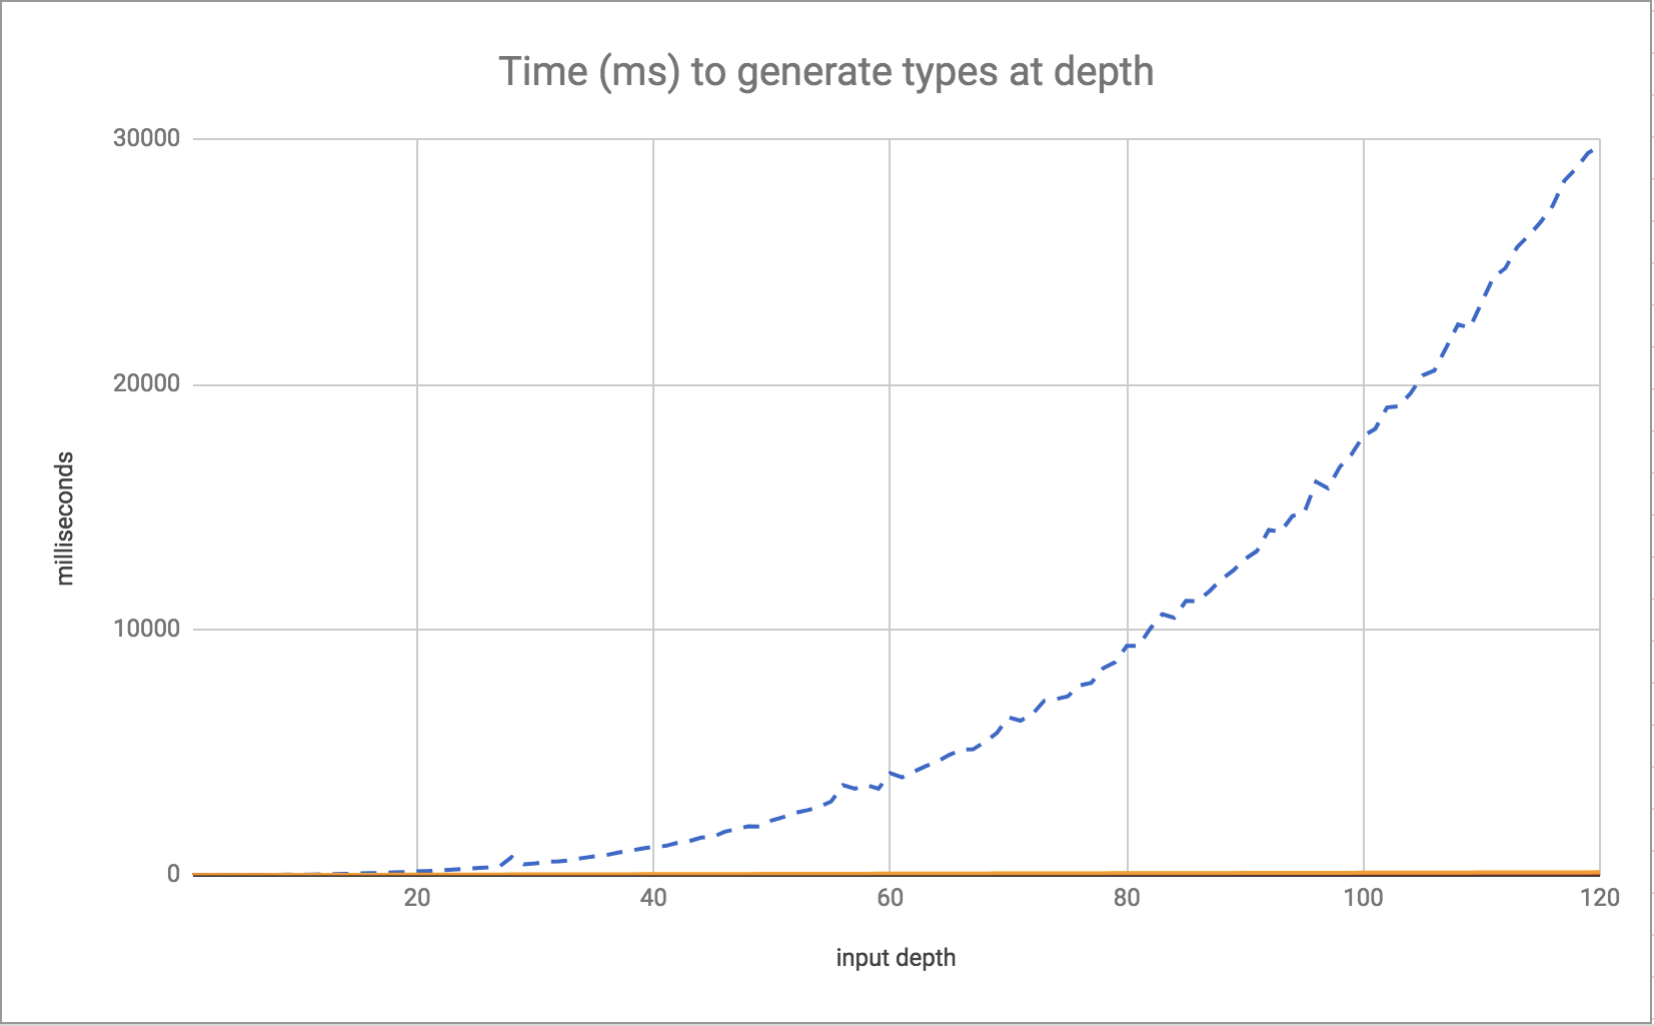
\includegraphics[width=\textwidth]{tagged-untagged-depth-bench120}

Benchmark 1 is represented by the red solid line, benchmark 2 by the
blue dotted line.

The graph shows the performance of Benchmark 1 is constant, because
the width of the largest union is always 2\ in an early phase of the reconstruction
algorithm.

The results for Benchmark 2 show the reconstruction algorithm is quadratic
with respect to the size of the largest union.

These observations are consistent with the prior theoretical analysis.

\Dsection{Can space use be bounded by reducing traces as collected?}

Traces in Typed Clojure's dynamic analysis are accumulated online, and then
folded into a type environment offline. However, this fold operation is commutative
with respect to the order of traces, so performing this fold online would
eliminate the need to store traces in memory.

Space is reduced further, then, by leveraging \texttt{join} to eagerly simplify
the accumulated type environment. For example, heterogeneous maps with similar
keysets could merged, possibily using optional key entries, saving space by
preventing very large redundant unions.

It is unclear if it is possible to perform more sophisticated analyses online,
in particular the recursive type reconstruction algorithm. Since the resulting
annotations are very compressed compared to intermediate points in the analysis,
fully or partially performing this analysis online may drastically decrease space
usage where recursively defined maps are used, and very deep examples are found.

\Dsection{Comparison to Daikon}

Daikon is a related system to Typed Clojure's dynamic type inference.
However, Daikon is built for ``invariant detection'', while our system
is designed for ``dynamic type inference'' or ``value profiling''.

There are two common implementation strategies for such tools. The first
strategy, ``ruling-out'' (for invariant detection), assumes all invariants are true 
and then use runtime analysis results to rule out
impossible invariants. The second ``building-up'' strategy (for dynamic type inference)
assumes nothing and then uses runtime analysis results to build up invariant/type knowledge.

Both strategies have different space behavior with respect to representing
the set of known invariants.
The ruling-out strategy typically uses a lot of memory at the beginning,
but then can free memory as it rules out invariants. For example, if
\texttt{odd(x)} and \texttt{even(x)} are assumed, observing \texttt{x = 1}
means we can delete and free the memory recording \texttt{even(x)}.
Alternatively, the building-up strategy uses the least memory storing
known invariants/types at the beginning, but increases memory usage
as more the more samples are collected. For example, if we know
\texttt{x : Bottom}, and we observe \texttt{x = "a"} and \texttt{x = 1}
at different points in the program, we must use more memory to
store the union \texttt{x : String $\cup$ Integer} in our set of known invariants.

Examples of invariant detection tools include Daikon \cite{Ernst06thedaikon},
DIDUCE \cite{hangal2002tracking}, and Carrot \cite{pytlik2003automated}, and
typically enhance statically typed languages with more expressive types or contracts.
Examples of dynamic type inference include Rubydust \cite{An10dynamicinference},
JSTrace \cite{saftoiu2010jstrace}, and TypeDevil \cite{pradel2015typedevil},
and typically target untyped languages.

%There is some overlap between invariant detection and dynamic type inference
%tools. Usually, invariant detection detects very expressive relationships
%between program variables; for example, for array \texttt{a} and index
%\texttt{i} variables, a derived invariant might be \texttt{0 < a[i]}.
%On the other hand, dynamic type inference (or value profiling) often just records
%basic nominal or structural type information---it is generally applied to untyped
%languages where basic static type information is absent.

\Dsubsection{Daikon's expressivity vs Typed Clojure's dynamic inference}

Daikon can reason about very expressive relationships between variables
using properties like ordering ($x < y$), linear relationships ($y = ax + b$),
and containment ($x \in y$). It also supports reasoning with ``derived variables''
like fields ($x.f$), and array accesses ($a[i]$).

Typed Clojure's dynamic inference can record heterogeneous data structures
like vectors and hash-maps, but otherwise cannot express relationships
between variables.

There are several reasons for this. The most prominent is that Daikon
primarily targets Java-like languages, so inferring simple type information
would be redundant with the explicit typing disciplines of these languages.
On the other hand, the process of moving from Clojure to Typed Clojure
mostly involves writing simple type signatures without dependencies
between variables. Typed Clojure recovers relevant dependent information
via occurrence typing, and gives the option to manually annotate necessary
dependencies in function signatures when needed.

\Dsubsection{Space/time overhead of Daikon's dynamic tracing}

Performance of dynamic tracing is not directly addressed in the Daikon
literature, who only provide complexity analyses and optimizations for storing
and checking invariants \emph{after} samples have been collected.

I have manually examined Chicory (the Java front-end to Daikon) to see how
dynamic tracing is implemented.
I found that Daikon records the value of all variables in scope
at each method entry/exit point \footnote{Implemented in \texttt{daikon.chicory.DaikonVariableInfo}}.
Then, to record values in Daikon, the following algorithm is used:

\begin{itemize}
  \item If the value is a Java primitive, record its value.
  \item If the value is an array, traverse its contents and record identity hash codes
    and/or primitive values.
  \item Otherwise, record the class of the current object.
\end{itemize}

Notice this algorithm is non-recursive---while arrays are traversed eagerly, they
are only traversed one level via an identity hash code summary (the closest equivalent to
pointer addresses on the JVM).
This is significantly different to Typed Clojure's value tracing algorithm,
which recursively (but lazily) traverses potentially-deep data structures.

Another difference is that Typed Clojure's dynamic tracing only tracks
values for arguments/returns of a function, and ignores any variables
that in are scope. There are several reasons behind this decision.
First, Java-like object-oriented languages use fields as implicit
arguments to methods, and Daikon distinguishes method-level, and class-level
invariants which is achieved by checking class-level invariants during
method calls.
In Clojure, methods are replaced with pure functions (their output is defined only by the
explicitly passed arguments), so the method/class-level distinction is
not applicable.

Second, Daikon chooses to reason about local mutation in Java-like languages,
and so must record the values of the same variables different program points
to observe mutation. However, local unsynchronized mutation is non-idiomatic
in Clojure so re-tracking variables is almost always redundant---mutation is
often via synchronized global variables that can be instrumented once-and-for-all.

\Dsubsection{Space/time overhead of Daikon's type inference}

The overhead of likely invariant detection
is described by Perkins and Ernst~\cite{Perkins04efficientincremental}.
They analyze the overhead of storing and checking the set of
invariants that are currently true.
Their presentation includes a simple incremental algorithm that
features no optimizations, then they propose several candidate
optimizations and empirically compare the performance of each
approach.

The space complexity of the simple incremental algorithm is dominated 
by the size of the grammar of properties. For example, if the grammar
of properties consists of $=$ and $even$, with
3 variables $x$, $y$, $z$, the initial (and largest) set of invariant assumptions
is $x = y$, $y = z$, $x = z$, $even(x)$, $even(y)$, and $even(z)$.
For reference, Daikon enables 152 properties by default, with
12 ``derived variables'', the latter of which provide properties on composite variables
like $a[x] = a[z]$. After a static analysis pass ruling out nonsensical invariants,
the space usage is at least $O(v^9)$, where $v$ is the number of variables in scope.

The time complexity of \emph{checking} invariants for each sample
is similarly dominated by the size of the grammar of properties.
They note, however, most invariants are removed quickly (after
$O(1)$ samples), so performance improves as more samples
are collected.

\Dsubsection{Checking Daikon's invariants in a refinement type system}

Daikon has expressive invariants, but can they be statically verified?
Yes, in fact Daikon supports generating annotations for a Java-based
theorem prover called Simplify~\cite{Detlefs03simplifya}.

Simplify implements the following theories.

1. The theory of equality, \texttt{=}

2. The theory of arithmetic with functions \texttt{+}, \texttt{*}, \texttt{-},
   and relation symbols \texttt{>}, \texttt{<}, \texttt{<=}, and \texttt{>=}.

3. The theory of maps with two functions \texttt{select} and \texttt{store} (ie. get/set),
   and two additional axoims.

4. Partial orders. % (?)

These could be encoded in Dependent Typed Racket, since it supports propositions
in linear arithmetic constraints about variables, pairs, car, and cdr.

% Notes:
%  Java implementation:
%    Chicory does instrumentation on JVM bytecode
%     instrument_all_methods: https://github.com/codespecs/daikon/blob/master/java/daikon/chicory/Instrument.java#L409
%      add_entry_instrumentation
%     - https://github.com/codespecs/daikon/blob/master/java/daikon/chicory/Instrument.java#L825
%      add_return_instrumentation
%       - instruments return statements
%      - https://github.com/codespecs/daikon/blob/master/java/daikon/chicory/Instrument.java#L675
%     daikon.chicory.Runtime
%      - contains wrappers for values that are rewritten to?
%      - Runtime.enter(...) is called at the top of every wrapped method
%      - `dtrace_writer` records inference results
%      daikon.chicory.DaikonVariableInfo
%      - actually traverses values here
%      - arrays are traversed eagerly, but only one level
%        - subsequent levels use identityHashCode summaries


\Dchapter{Conclusion}

This paper shows how to
generate recursive heterogeneous type annotations for
untyped programs that use plain data.
We use a novel algorithm to ``squash'' the observed structure
of program values into named recursive types suitable for
optional type systems,
all without the assistance of record, structure, or class
definitions.
We test this approach on thousands of lines of Clojure code,
optimizing generated annotations
for programmer comprehensibility over soundness.

In our experience, our guidelines
to automatically name, group, and reuse
types yield insightful annotations
for those with some familiarity with
the original programs,
even if the initial annotations are imprecise, incomplete,
and always require some changes to type check.
Most importantly, many of these changes will involve simply rearranging or changing parts
of existing annotations, so programmers are no longer left alone
with the daunting task of reverse-engineering such programs
completely from scratch.

%Our generated annotations
%serve as a valuable starting point for annotating untyped programs
%who rely on plain data, especially

%We indend to convey to programmers
%to understand 
%
%and report on experience in using our tool to generate annotations for real-world
%Clojure programs, and enumerate the remaining changes needed to fully port
%them to Typed Clojure.
%
%Optional type systems 
%were created on the observation
%that even dynamic programming languages have a 
%
%We tackle the problem of 
%Our approach to automatically
%generate recursive types from unrolled examples,
%has proven
%even with the challenge of 
%
%% key insights
%% - recursive annotations for records and classes without declarations.
%% - how to recover the structure from class definitions
%%   without programmer intervention?
%% - generalized types 
%
%We have tested our approach on thousands of lines
%of Clojure code,
%Typed Clojure types for Clojure
%programs. Despite the fact that Clojure programs
%declare minimal structure, we successfully 


% Quals
%\part{Investigation of clojure.spec}
%\label{part:spec}
%
%%\subsection{Overview of clojure.spec}
%
%This thesis claims that we can automatically generate annotations to other verification
%systems similar to Typed Clojure.
%We add a second usecase to strengthen our claim: generating annotations for \texttt{clojure.spec},
%a runtime verification library recently added to Clojure's core library.
%It resembles common approaches to runtime verification, such as Racket's contract
%system, but is different in several important ways.
%
%Firstly, \texttt{clojure.spec} is designed to treat most values as ``data at rest''. That is,
%at verification sites, values are eagerly traversed without waiting to see
%if or how the program actually uses them.
%When we consider that \texttt{clojure.spec} treats infinite streams
%and functions as data at rest, we begin to see the tradeoffs that have been
%made.
%
%Secondly, specifications (called ``specs'') are not enforced by default. Users must
%opt-in to enforcing specs via an explicit instrumentation phase.
%This is also different than most contract systems, many of which are enforced
%by default. There is no standard way to integrate spec enforcement into a
%test suite, so it is difficult to tell whether specific specs are primarily 
%unchecked documentation, or actually used for runtime verification.
%
%Since \texttt{clojure.spec} has a unique feature set amongst runtime verification
%libraries, it is interesting to consider how programmers use \texttt{clojure.spec}
%in practice. For example, do programmers find the semantics of treating functions
%as data at rest useful?
%
%%Unfortunately since specs are opt-in, it is difficult to
%%correlate someone writing a spec with that person \emph{using} the spec,
%%implying spec's semantics as being useful.
%%Nevertheless, in the following sections we attempt to draw conclusions about
%%spec's common usage based mostly on the frequency of spec annotations.
%
%\subsection{Function specifications in clojure.spec}
%
%We now give a brief introduction to what using clojure.spec is like,
%focussing on the semantics of the different kinds of function specifications
%it supports.
%
%(From here, we map the namespace prefix \texttt{s} to \texttt{clojure.spec.alpha},
%and \texttt{stest} to \texttt{clojure.spec.test.alpha}.)
%
%\begin{verbatim}
%(require '[clojure.spec.alpha :as s])
%(require '[clojure.spec.test.alpha :as stest])
%\end{verbatim}
%
%There are two kinds of function checking semantics in \texttt{clojure.spec}.
%We use \texttt{intmap}, a higher-order function that maps a function over 
%a collection of ints, to demonstrate both semantics.
%
%\begin{verbatim}
%(defn intmap
%  "Maps a collection of ints over a function."
%  [f c]
%  (map f c))
%\end{verbatim}
%
%If the programmer wants to write a higher-order function spec to
%verify \texttt{intmap}, they might write the following spec.
%
%\begin{verbatim}
%(s/fdef intmap
%  :args (s/cat :f (s/fspec :args (cat :x int?) :ret int?)
%               :c (s/coll-of int?))
%  :ret (s/coll-of int?))
%\end{verbatim}
%
%The \texttt{s/fdef} form signals we are annotating a top-level
%function, in this case \texttt{intmap}. Argument specs are
%provided with the \texttt{:args} keyword option
%in the form of the ``tagged'' heterogeneous collection spec
%\texttt{s/cat}---here 2 arguments are allowed, tagged as
%\texttt{:f} for the function and \texttt{:c} as the collection.
%
%The \texttt{s/fspec} spec is another kind of function spec,
%specifically for non-top-level functions (such as function arguments
%to top-level functions). It has a similar syntax to \texttt{s/fdef},
%but a function name is not provided.
%
%In a nutshell, \texttt{s/fdef} provides traditional proxy-based
%verification semantics while \texttt{s/fspec} uses eager \emph{generative testing}
%to exercise a function before letting it pass the spec boundary, bare (without a proxy).
%
%We will now demonstrate how the following call gets checked.
%
%\begin{verbatim}
%(intmap inc [1 2 3])
%;=> (2 3 4)
%\end{verbatim}
%
%First, the programmer instruments \texttt{intmap} with:
%
%\begin{verbatim}
%(stest/instrument `intmap)
%\end{verbatim}
%
%This mutates the top-level binding associated with \texttt{intmap}, wrapping a function
%proxy around the original value.
%
%Now, when checking \texttt{(intmap inc [1 2 3])}, the \texttt{inc} function is
%called several hundred times with generated values conforming to \texttt{int?},
%and checks each call returns an \texttt{int?}.
%Then, \texttt{[1 2 3]} is eagerly checked against \texttt{(s/coll-of int?)}.
%The original \texttt{intmap} function is then called with the original arguments,
%yielding a value \texttt{(2 3 4)}. Instrumentation does not check return value specs,
%so \texttt{(s/coll-of int?)} is ignored, and the original return value is passed to the calling
%context.
%
%\subsection{Automatic Annotations for clojure.spec}
%
%Having introduced \texttt{clojure.spec}, we now give an overview
%of how to repurpose our automatic annotation technology to generate specs.
%At a glance, the problems of generating annotations for Typed Clojure
%and \texttt{clojure.spec} are similar, and indeed we can reuse much
%of the machinery from our approach to generating Typed Clojure annotations.
%The differences lie mostly in the finally type reconstruction phase.
%
%There are several important components in \texttt{clojure.spec}'s
%philosophy and design that complicate its annotation story.
%First, \texttt{clojure.spec} does not support local key-type pairs
%in its heterogeneous map specification--instead you are forced
%to globally define map entries as \emph{spec aliases}.
%
%For example, the Typed Clojure type \clj{'\{:a Int\}} must be
%written \clj{(s/keys :req-un [:my-ns/a])}, along with the following
%global definition of the spec alias \clj{:my-ns/a}.
%\begin{verbatim}
%(s/def :my-ns/a int?)
%\end{verbatim}
%When \clj{(s/keys :req-un [:my-ns/a])} is checked against a value,
%it first locates the spec under \clj{:my-ns/a}, and (because
%we have declared the key to be \clj{:req-un}, that is, required
%but unqualified), we use the located \clj{int?} spec
%to check against the \clj{:a} entry of the value.
%Furthermore, if the key was declared as \clj{:req} instead of \clj{:req-un},
%the fully qualified keyword entry \clj{:my-ns/a} would be checked
%against \clj{int?}.
%This means that there is \emph{exactly one} spec for each fully
%qualified keyword entry.
%
%This raises several interesting design issues related to reusing
%specs that are very different from the simpler problem of generating
%Typed Clojure \clj{HMap} types. 
%How do we decide which namespace to register unqualified map entries?
%Should we assume similar looking keyword entries are in fact the same, and register their specs under the same namespace?
%How do we handle fully qualified keyword entries?
%
%The second component of

%\chapter{Clojure.spec Study}

\section{Research questions}

I aim to answer these research questions:

\begin{itemize}
  \item What does the frequency and applications of \texttt{fdef} and \texttt{fspec} specs
    in open source software reveal about the utility of \texttt{clojure.spec}'s
    function semantics in practice?
\end{itemize}

I do not attempt to answer the following questions:

\begin{itemize}
  \item How frequently do users instrument specs for runtime verification?
\end{itemize}

\section{Methodology}

\subsection{Sources}

To determine the frequency of \texttt{fdef} and \texttt{fspec} specs,
the search features of \texttt{GitHub}~\footnote{\texttt{https://github.com}} and 
\texttt{CrossClj}~\footnote{\texttt{https://crossclj.info}} were used.

GitHub indexes tens of thousands of open source Clojure projects, and provides
a rudimentary search interface that is sufficient for discovering textual occurrences 
of functions and macros. False positives are common however, such as
GitHub does not distinguish
between ``toy'' projects and those with official releases, so we remove the former manually.
This is because toy projects do not give a good indication of real-world idioms---for example,
hundreds of projects simply contain experiments with \texttt{clojure.spec} that
are not officially released or maintained.

CrossClj maintains a rich database of cross-links between Clojure projects.
As of Febuary 2018, it indexes 9,438 projects, all of which have official releases (unlike
GitHub search) and thus have more credibility that they are used.
Cross-links are gathered for function/macro usages, and transitive project dependencies.
Unlike GitHub, CrossClj also distinguishes between ClojureScript and Clojure code

\subsection{Frequency Data gathering}

Simple GitHub searches were used to find occurrences of \texttt{fdef} and \texttt{fspec}.
As of March 2018,
searches for \texttt{fdef}
yield around 2,000 results~\footnote{\texttt{https://github.com/search?q=fdef+language\%3Aclojure\&type=Code}},
and for \texttt{fspec} 
\footnote{\texttt{https://github.com/search?q=fspec+language\%3Aclojure\&type=Code}}
yield around 600 results.
Searches were quite noisy, so less actual examples of these forms were found.

As a baseline, we searched for several common spec forms.
The spec \texttt{def} form for defining spec aliases found around 4,400 results.
The spec \texttt{keys} form for heterogeneous maps found around 3,500 results.
All of these numbers are compared in Figure~\ref{frequencybargraphs}.

CrossClj function/macro cross-links were used to find occurrences of spec idioms.
From the latest index (updated February 20th 2018)
\texttt{fdef} occurs in 721 top-level forms over 83 
projects~\footnote{\texttt{https://crossclj.info/fun/clojure.spec.alpha/fdef.html}}, and
\texttt{fspec} occurs in 22 top-level forms over 8 
projects~\footnote{\texttt{https://crossclj.info/fun/clojure.spec.alpha/fspec.html}}
(the mode number of occurrences per project was 1).

An error was found in the CrossClj data, however.
To find a baseline number of projects using \texttt{clojure.spec}, we looked for occurrences of
\texttt{s/def}, used to define spec
aliases. It should greatly outnumber the number of \texttt{fdef}'s in the ecosystem---we were
surprised to find CrossClj reports the opposite, and
we are almost certain these particular CrossClj metrics are incorrect.
We identified that multiple occurrences of \texttt{s/def} in the same project are not always counted by CrossClj,
so while CrossClj claims \texttt{s/def} occurs in more 60\% more projects than \texttt{fdef} (125), 
CrossClj reports \texttt{s/def} only occurs in 349 top-level 
forms~\footnote{\texttt{https://crossclj.info/fun/clojure.spec.alpha/def.html}}.
The latter number is too low---CrossClj reports, for example, the \texttt{clj-time}
library only has 2 occurrences of \texttt{s/def}, but it actually has 7 occurrences.

\begin{figure}
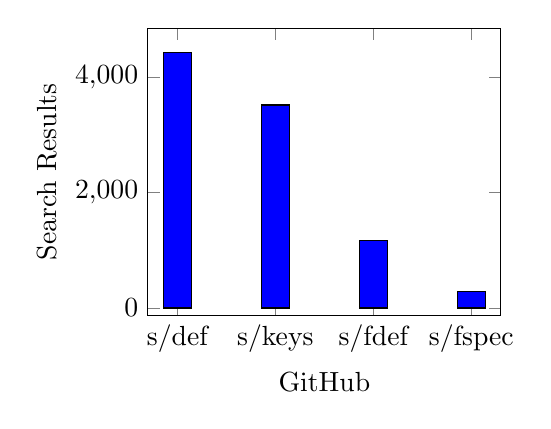
\begin{tikzpicture}
\begin{axis}[
  width=0.5\textwidth,
  symbolic x coords={s/def,s/keys,s/fdef,s/fspec},
    ylabel=Search Results,
    xlabel=GitHub,
    xtick=data]
    \addplot[ybar,fill=blue] coordinates {
         (s/def,4439)
         (s/keys,3522)
         (s/fdef,1167)
         (s/fspec,286)
                   };
\end{axis}
\end{tikzpicture}
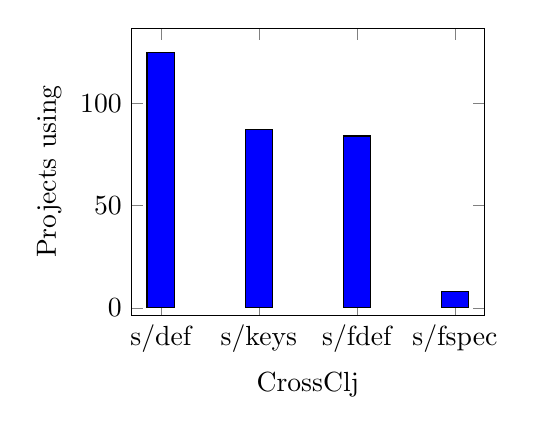
\begin{tikzpicture}
\begin{axis}[
  width=0.5\textwidth,
    symbolic x coords={s/def,s/keys,s/fdef,s/fspec},
    ylabel=Projects using,
    xlabel=CrossClj,
    xtick=data]
    \addplot[ybar,fill=blue] coordinates {
         (s/def,125)
         (s/keys,87)
         (s/fdef,84)
         (s/fspec,8)
                   };
\end{axis}
\end{tikzpicture}
\caption{Left, the number of results for GitHub searches about spec forms.
Right, the number of projects on CrossClj that use spec features.
  Searches for \texttt{ifn?} are omitted because
  it has been used as a common predicate since before 2009 (spec was released in 2017).
  }
  \label{frequencybargraphs}
\end{figure}

We did not notice such an error in the counts for \texttt{fspec} and \texttt{fdef}, but
this error reduces confidence on the exact numbers. Interestingly, the \emph{relative}
numbers of projects using these forms matches our intuition---\texttt{fspec} occurs
10 times less often than \texttt{fdef}, and \texttt{fdef} occurs about half as often as \texttt{s/def}
(see plot in Figure~\ref{frequencybargraphs}).
Still, these numbers should be treated with suspicion.

\subsection{Project Samples}

We selected 18 open source projects that use \texttt{fspec} to manually examine.
They were chosen by first searching GitHub for \texttt{fspec} occurrences, and
manually choosing the first few dozen results, manually keeping only projects
seemed to have official releases.
Figure~\ref{fspectable} summarizes these findings. We have included the project
names and our scratch notes as Appendix~\ref{appendix1}.

We also searched for negative examples of \texttt{fspec} usage---that is, occurrences
of higher-order functions with specs that did not use \texttt{fspec}---by searching for
both \texttt{fdef} and 
\texttt{ifn?}~\footnote{\texttt{https://github.com/search?utf8=\%E2\%9C\%93\&q=ifn\%3F+fdef+language\%3Aclojure\&type=Code}}, 
the flat contract for Clojure functions.
We selected 17 projects using a similar method via a GitHub search.
Appendix~\ref{appendix2} contains the projects and our scratch notes for this experiment.

\section{Experiment 1: Frequency of \texttt{fspec}}
\label{experiment1}

\begin{figure*}[t]

\begin{tabular}{lll}
      \toprule
  & \texttt{fspec} & \texttt{ifn?} \\
  \midrule
  Total occurrences in \texttt{fdef} & 79 & 3 \\
  \tabitem
  Total occurrences in \texttt{fdef} arguments & 65 (82\%) & 3 \\
  \tabitem
  Total occurrences in \texttt{fdef} return & 14  (18\%) & 0 \\
  Total occurrences in map spec & 41 & 2 \\
  \tabitem
  Total occurrences in heterogeneous map spec & 40 (97\%) & 2 \\
  \tabitem
  Total occurrences in homogeneous map spec & 1 (3\%) & 0 \\

\end{tabular}
\caption{Function specs in practice, in 18 open source projects sourced from GitHub that utilized \texttt{fspec}. }
\label{fspectable}
\end{figure*}

Our first investigation concentrated on projects that use \texttt{fspec}.
We chose 18 open source projects and manually investigated their usage of spec.

To gauge how \texttt{fspec}s are used in practice, we divided their occurrences
into several categories. 
Figure~\ref{fspectable} presents the results.

First, we measure how many times \texttt{fspec} occurs in top-level function
specs (i.e., \texttt{fdef} forms). Because spec has different semantics for
checking the argument and return of top-level function specs, we split this
category into occurrences in the arguments spec and return spec.
We also similarly measure the occurrences of \texttt{ifn?} in these projects,
which was sparsely used in these projects.

We found 82\% \texttt{fspec} instances occuring in the argument position,
with 18\% in the return position.

Second, we measure the frequency of \texttt{fspec} in a hash-map spec.
Of the occurrences of \texttt{fspec} in map specifications, 
we found a strong preference for using heterogeneous map specs (97\%),
with the rest being homogeneous maps.
If \texttt{fspec} occurs in a nested map, each map spec occurrence is counted.
Similar to the previous experiment, the flat function contract \texttt{ifn?} was rarely used 
in map specs in these projects.

We noticed several interesting things while conducting these experiments.

There was only 2 occurrence of nesting function specs more than 2 deep---in a library
that provides functional lenses~\footnote{https://github.com/andrewmcveigh/bifocal}.
Of those, one used 3 \texttt{fspec}s, the other 2 \texttt{fspec}s with a terminating \texttt{ifn?}.

We also noticed several users combining \texttt{fspec}s with the \texttt{or} spec
for disjunctions. It's unclear how well this works in practice (and might only be
there for documentation), but the ``looser'' generative testing semantics of \texttt{fspec}
seems to have more compatibility with disjunction contracts than the ``stricter''
proxy-based verification approach.

Spec also provides the ability to write dependent function contracts via the \texttt{:fn}
keyword option of \texttt{fspec}, allowing programmers
to add custom code to verify the relationship between function arguments and return values.
We found several interesting dependent contracts that used surprising techniques like
memoization to verify calls to higher-order functions~\footnote{https://github.com/CharlesHD/chu.graph}.

Some developers explicitly worked around the \texttt{fspec}'s generative testing semantics.
We found several comments and workarounds explaining why \texttt{fspec}s were not
appropriate in particular contexts. Common concerns were
\\
\begin{itemize}
	\item triggering function side effects,
	\item difficultly writing generators for testing the function, and
	\item being unsure whether generative testing was appropriate.
\end{itemize}

We speculate the lack of polymorphic function specs contributed to these concerns.
Since instances of a type variable were replaced with \texttt{any?} specs, writing
a generator often did not make sense. It's unclear whether polymorphic specs are
even feasible to check, but some developers at least seem attached to the documentation
capabilities of \texttt{fspec}, perhaps suggesting more control over the testing
semantics of \texttt{fspec} would be welcomed by spec users.

% function nesting:
% - lens library had largest nesting
% - depth 3 fspec's
% - depth 2 fspec's + terminating ifn?

\section{Experiment 2: Frequency of \texttt{ifn?}}
\label{experiment2}

\begin{figure*}[t]

\begin{tabular}{lll}
      \toprule
  & \texttt{fspec} & \texttt{ifn?} \\
  \midrule
  Total occurrences in \texttt{fdef} & 0 & 188 \\
  \tabitem
  Total occurrences in \texttt{fdef} arguments & 0 & 170 (90\%)\\
  \tabitem
  Total occurrences in \texttt{fdef} return & 0 & 18 (10\%)\\
  Total occurrences in map spec & 0 & 173 \\
  \tabitem
  Total occurrences in heterogeneous map spec & 0 & 67 (39\%) \\
  \tabitem
  Total occurrences in homogeneous map spec & 0 & 106 (61\%)\\

\end{tabular}
\caption{Flat function specs in practice, in 17 open source projects sourced from GitHub that utilized \texttt{ifn?}.
The 106 homogeneous map spec occurrences were sourced from only 3 of the projects, one project contributing the maximum 93 occurrences.
Heterogeneous map specs occurrences were from 7 of the projects, with maximum 30 occurrences in one project.
}
\label{ifntable}
\end{figure*}

In our second experiment, we measured the frequency of \texttt{ifn?} in 17 open source projects.
The results are summarised in Figure~\ref{ifntable}.

Similar to our first experiment, occurrences of \texttt{ifn?} were mostly in the argument
positions in \texttt{fdef} (90\%).
The data for \texttt{ifn?} occurrences in map specs is somewhat skewed, since one project
contributed over half of the occurrences. However, even without taking that project into account,
around half of all the \texttt{ifn?} occurrences were found in map specs.

One striking divide we noticed was the obvious preference for either \texttt{ifn?} or \texttt{fspec}
per project. None of the projects that primarily used \texttt{ifn?} used \texttt{fspec} even once.
In the first experiment, projects that used \texttt{fspec} used \texttt{ifn?} rarely---mostly to
avoid \texttt{fspec}'s generative testing semantics.

\section{Conclusions}

Our goal in this section was to inform our decisions for when to generate \texttt{fspec}
annotations in our automatic spec annotation tool.
We surveyed open source projects via GitHub by measuring instances of two kinds of projects:
those that primarily used \texttt{fspec}, and those that primarily used \texttt{ifn?}.

Our experiments yielded many interesting insights. Even using broad measurements like
GitHub searches and CrossClj project references,
we consistently found other common spec features were used roughly an order of
magitude more than \texttt{fspec} (Figure~\ref{frequencybargraphs}).

However, we still investigated how programmers use \texttt{fspec} (Section~\ref{experiment1}).
In the projects that primarily used \texttt{fspec} for first-class function specs,
we found several instances of programmers enjoying the expressive documentation
of \texttt{fspec}, but avoiding its generative testing semantics in creative ways.
Sometimes \texttt{fspec}s commented out and replaced with \texttt{ifn?}, implying
spec might benefit from more control over \texttt{fspec}'s testing semantics.

Our second experiment (Section~\ref{experiment2}) measured how programmers combined
spec with \texttt{ifn?}.
Interestingly, none of the 17 projects we selected used \texttt{fspec}---programmers
seem divided in strong preferences for \texttt{ifn?} and \texttt{fspec}, with
\texttt{fspec} users using \texttt{ifn?} only occasionally to work around
\texttt{fspec}'s testing semantics.

A unique feature of spec's runtime instrumentation of \texttt{fdef}s is that
return values are not checked. Since we predicted programmers might have
issues with \texttt{fspec}'s generative testing semantics, we were interested
if \texttt{fspec}'s were more frequent than usual in the return position
of \texttt{fdef} (where these semantics would be implicitly suppressed).
In our investigation, we found no particular evidence that programmers preferred
\texttt{fspec} over \texttt{ifn?} in the return position---when they occurred in \texttt{fdef} forms,
\texttt{fspec} was in the return position 18\% of the time (Figure~\ref{fspectable}),
and \texttt{ifn?} was 10\% of the time (Figure~\ref{ifntable}).

One difference we found was \texttt{ifn?} occurs with a high correlation in
a map spec (92\% of the time), while \texttt{fspec} occurred in a map spec
only 51\% of the time.
However, \texttt{fspec} occurred much more often in heterogeneous map specs
(97\% of occurrences in map specs were heterogeneous), while \texttt{ifn?}
only occurred in heterogeneous maps 39\% of the time.
Heterogeneous maps in Clojure are used like records or structs in other
languages~\cite{bonnaire2016practical}, so the appeal of combining
\texttt{fspec} with heterogeneous maps is similar to giving precise annotations
to record or struct fields.

The lack of polymorphism in spec coupled with the frequency of polymorphic functions
in Clojure seems to be a strong reason to prefer \texttt{ifn?} in many situations.
We found \texttt{ifn?} was often used to avoid ``any to any'' function
specs, which would otherwise use the generator for \texttt{any?} to generatively test
the function value. This is inappropriate for many common variants on polymorphic functions like
\texttt{map}, \texttt{filter}, and \texttt{reduce}
and we found several examples in our experiments that support this view
(see occurrences of ``polymorphic'' in Appendix~\ref{appendix2}).

% how does no polymorphism interact with fspec semantics? are they more useful together?

To tie back our investigation---what does this tell us about programmer preferences in an automatic spec annotation
tool? At the very least, it tells us there is no simple ``fits all'' behavior---we found
preferences were in (at least) two distinct camps.
This implies that the tool should have some customizability between preferring
\texttt{fspec} and \texttt{ifn?}, but which should be the default?

Should the tool prefer more expressive, but possibly incorrect specs, over less
expressive but specs that ``just work''?
I don't think there is a single definitive answer---rather each occurrence of \texttt{fspec}
comes with its own context and tradeoffs. Whether it occurs in the arguments or return of
an \texttt{fdef}, in a heterogeneous or homogeneous map, or even nested in another \texttt{fspec}
are relevant contextual information that the default behavior of the tool should take
into account. The varied and subtle results of this investigation support the conclusion
that the tool's behavior should probably itself be varied and subtle.


%\chapter{Formal model of Clojure.spec}

%\begin{verbatim}
%Write a formal model of Clojure with core.spec, and implement it in
%PLT Redex. Formulate a consistency property between contracted and
%uncontracted execution, and test it in redex.
%\end{verbatim}
%
%\input{syntax-figure-lambdac}

We devise a base formal model for Clojure called \lambdac{}
(syntax defined in Figure~\ref{clojure-grammar}).
We extend \lambdac{} with clojure.spec with \texttt{fdef} but without 
\texttt{fspec} specs, and call
this model \lambdacs{}
(syntax defined in Figure~\ref{clojurespec-grammar}).
Then, we extend \lambdacs{} to support
\texttt{fspec} function contracts, and call this final model \lambdacsf{}
(syntax defined in Figure~\ref{clojurespechof-grammar}).

We define the small-step reduction rules ($\rightarrow$) for each language, using contexts.
Figure~\ref{arrowv} defines the reduction rules for 
the base language \lambdac{}---it does not include any spec features.
Figure~\ref{arrowvspec} defines the reduction rules for 
\lambdacs{}, adding support for \texttt{fdef}.
Finally, Figure~\ref{arrowvspec-hof} defines the reduction rules for 
\lambdacsf{}, adding support for \texttt{fspec}.

\section{Consistency property}

Let $\rightarrow^{*}$ be the reflexive, transitive closure of $\rightarrow$,
the single-step reduction relation for our respective languages.

We formulate two consistency properties, one which we expect to hold, another
which does not hold, and test them both using Redex.

The first theorem (Theorem~\ref{th1}) states that any expression in \lambdac{}
evaluates to the same value (or error) as checking that value against
any spec in \lambdacs{}, or throws a spec value.
For example, \texttt{1} in \lambdac{} evaluates to the same value (or error)
as \texttt{(assert-spec 1 number?)}. Furthermore, \texttt{(assert-spec 1 zero?)} 
evaluates to a spec error, and so is also consistent with \texttt{1}
in \lambdac{}.

\begin{theorem}[Consistency without fspec]
\label{th1}
For every expression \texttt{E} in \lambdac{}, 
and every spec $\mathbb{S}$ in \lambdacs{}, 
if \texttt{E} $\rightarrow^{*}$ $\texttt{V}_1^{e}$ and
\texttt{(assert-spec E $\mathbb{S}$)} $\rightarrow^{*}$ $\texttt{V}_2^{e}$,
then either:
\begin{itemize}
\item $\texttt{V}_1^{e} = \texttt{V}_2^{e}$, or
\item $\texttt{V}_2^{e}$ is \texttt{(error spec-error ...)}.
\end{itemize}
\end{theorem}

We formulated Theorem~\ref{th1} in Redex, and tested it for 1000 expressions,
each with 1000 specs. We found no counter-examples, as expected.

We expect to find a counter-example in Theorem~\ref{th2}, however.
It is similar to Theorem~\ref{th1}, except we compare \lambdac{} with
\lambdacsf{}, which includes \texttt{fspec}s (with generative testing semantics).

\begin{theorem}[Consistency with fspec]
\label{th2}
For every expression \texttt{E} in \lambdac{}, 
and every spec $\mathbb{S}$ in \lambdacsf{}, 
if \texttt{E} $\rightarrow^{*}$ $\texttt{V}_1^{e}$ and
\texttt{(assert-spec E $\mathbb{S}$)} $\rightarrow^{*}$ $\texttt{V}_2^{e}$,
then either:
\begin{itemize}
\item $\texttt{V}_1^{e} = \texttt{V}_2^{e}$, or
\item $\texttt{V}_2^{e}$ is \texttt{(error spec-error ...)}.
\end{itemize}
\end{theorem}

Formulating Theorem~\ref{th2} in Redex finds many counter-examples
involving \texttt{fspec}.
For example, the following call that generates only 10 expressions each with 10
random specs finds a ``stuck'' term from trying to generatively test a one-argument
function \texttt{boolean?} as if it had zero-arguments (there is no way to know
a function's arity in advance).

\begin{verbatim}
> (check-Clojure-ClojureSpecHOF-compat 10 10)
ERROR:
ClojureSpec evaluation did not fully reduce
Original-form: (assert-spec boolean? (FSpec () zero? 0))
Stuck-form: (assert-spec boolean? (FSpec () zero? 0))
\end{verbatim}

\section{Notes on Redex model}

Caching was disabled for the Redex model because it interfered with generative testing.
For example, the result of \texttt{(gen-spec number?)} was cached, so generative testing coverage
was very poor.

The model rendered in this paper can be found at:
\begin{itemize}
\item \texttt{https://github.com/frenchy64/quals/blob/master/redex/clj2.rkt}.
\end{itemize}

For experimentation, the same model, but based on the Eval-Apply-Continue machine
can be found at:
\begin{itemize}
\item
 \texttt{https://github.com/frenchy64/quals/blob/master/redex/clj.rkt}.
\end{itemize}

\begin{figure*}
\fbox{
  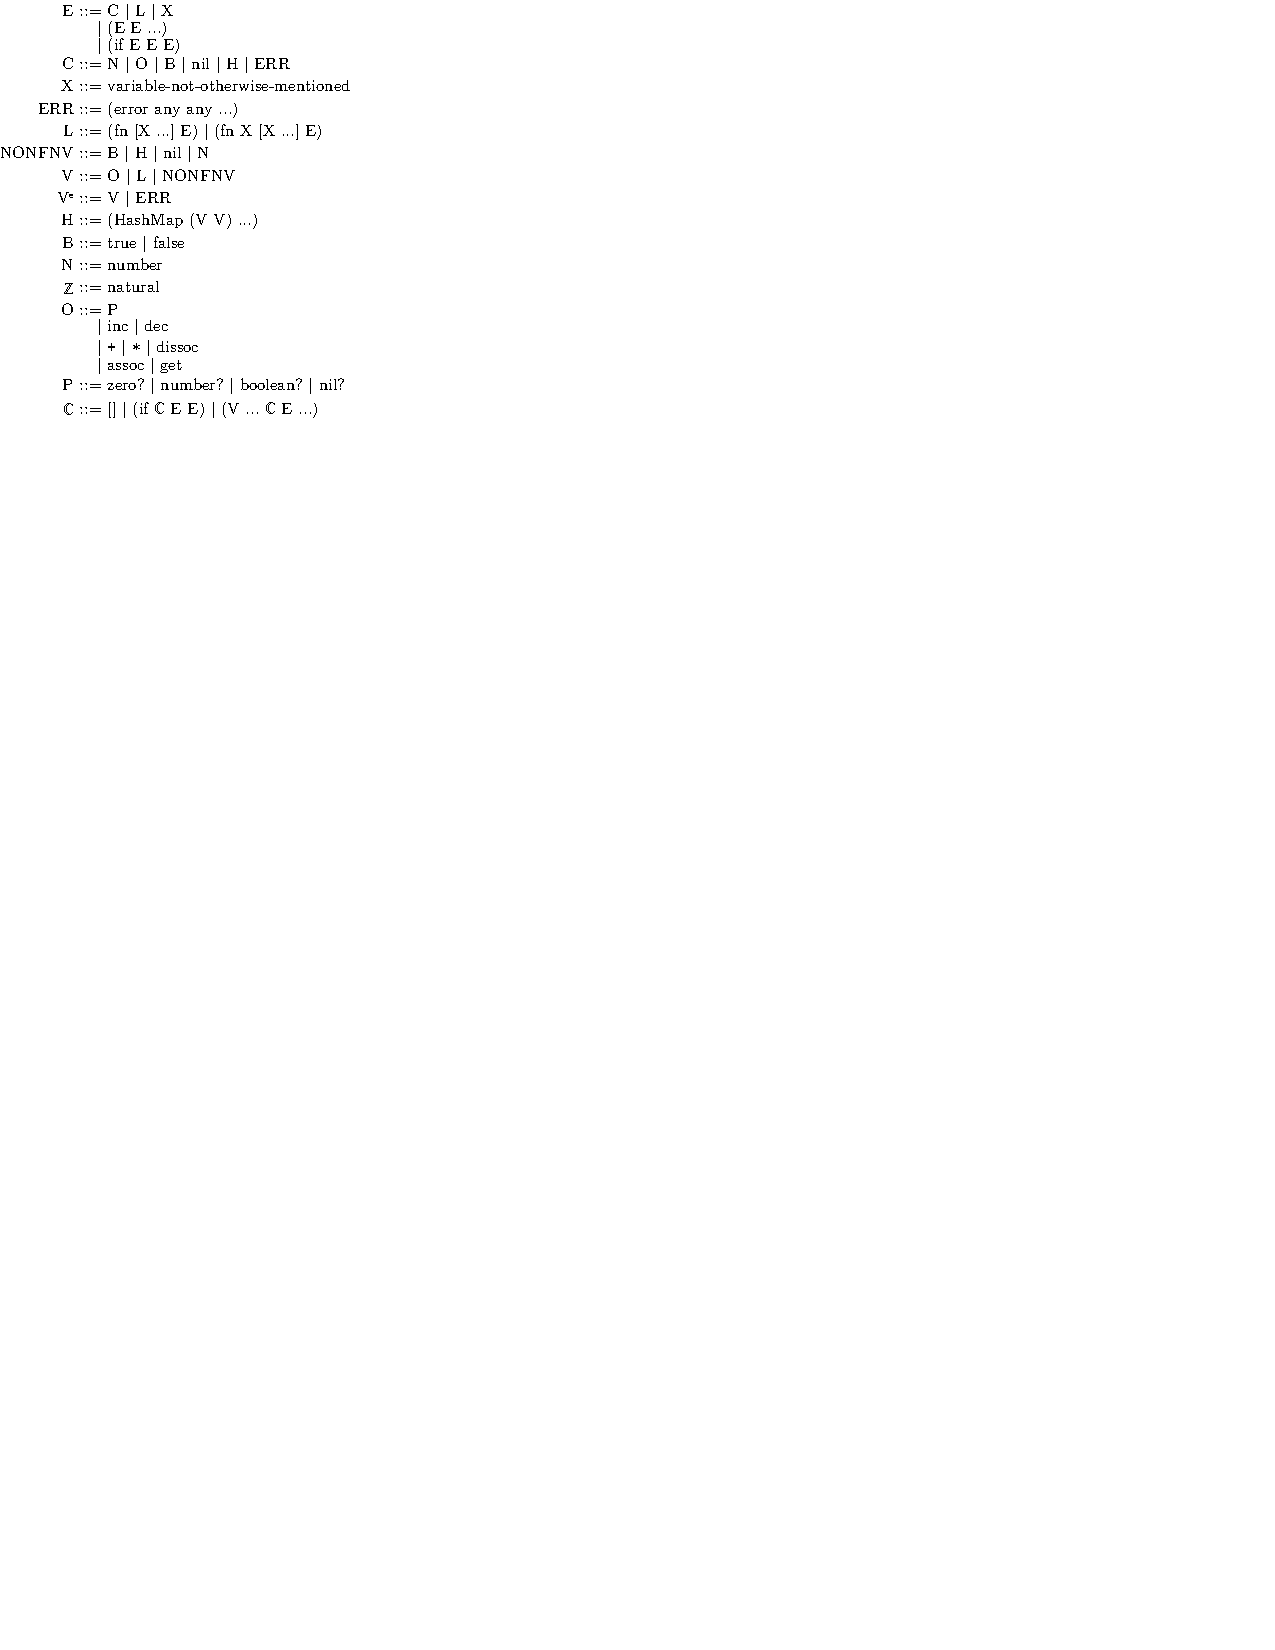
\includegraphics[]{redex/clojure-grammar.pdf}
}
\caption{Syntax of Terms in $\lambda c$.
  Expressions \texttt{E} consist of (loosely named) ``constant'' expressions \texttt{C}
  (numbers \texttt{N}, built-in functions \texttt{O}, booleans, nil, hash maps \texttt{H}, and errors
\texttt{ERR}), 
  functions \texttt{L} (non-recursive, and recursive), variables \texttt{X}, applications,
  and conditionals.
  The built-ins \texttt{assoc}, \texttt{dissoc}, and \texttt{get} perform the
  hash map operations add, remove, and lookup, respectively.
  Values are denoted \texttt{V}, and we use contexts $\mathbb{C}$ to define reduction rules.
  }
  \label{clojure-grammar}
\end{figure*}

%\input{syntax-figure-lambdacs}

\begin{figure*}
\fbox{
  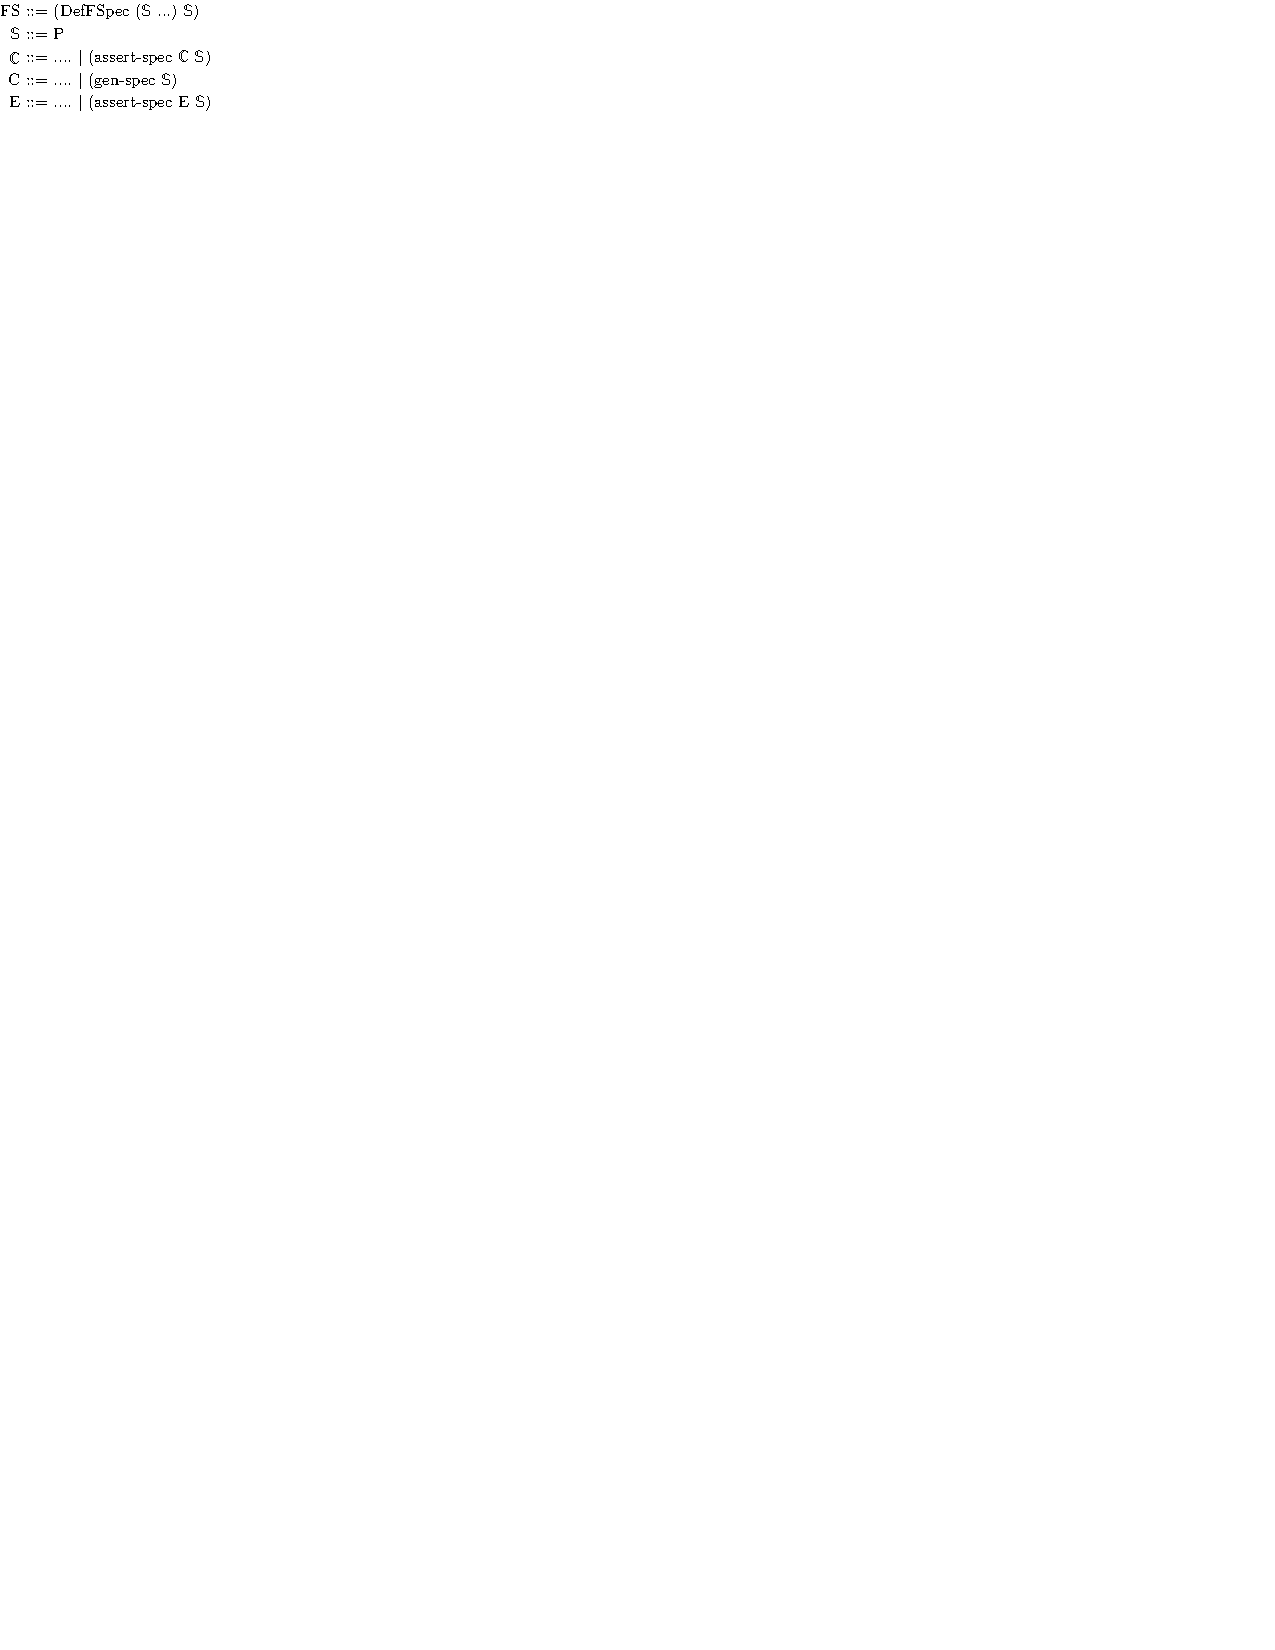
\includegraphics[]{redex/clojurespec-grammar.pdf}
}
\caption{Syntax of $\lambda c_s$ (extending $\lambda c$, Figure~\ref{clojure-grammar}).
  We add the \texttt{assert-spec} form that takes an expression and a spec
  and checks the expression evaluates to a value conforming to the spec.
  We restrict specs to just predicates \texttt{P}.}
  \label{clojurespec-grammar}
\end{figure*}

%\input{syntax-figure-lambdacsf}
\begin{figure*}
\fbox{
  
\includegraphics[]{redex/clojurespechof-grammar.pdf}
}
\caption{Syntax of $\lambda c_s^f$ (extending $\lambda c_s$, Figure~\ref{clojurespec-grammar}).
  We add two forms of \texttt{fspec}s---the natural number represents how
  many times to generatively test a function value.
  }
  \label{clojurespechof-grammar}
\end{figure*}

\begin{figure}
\fbox{
  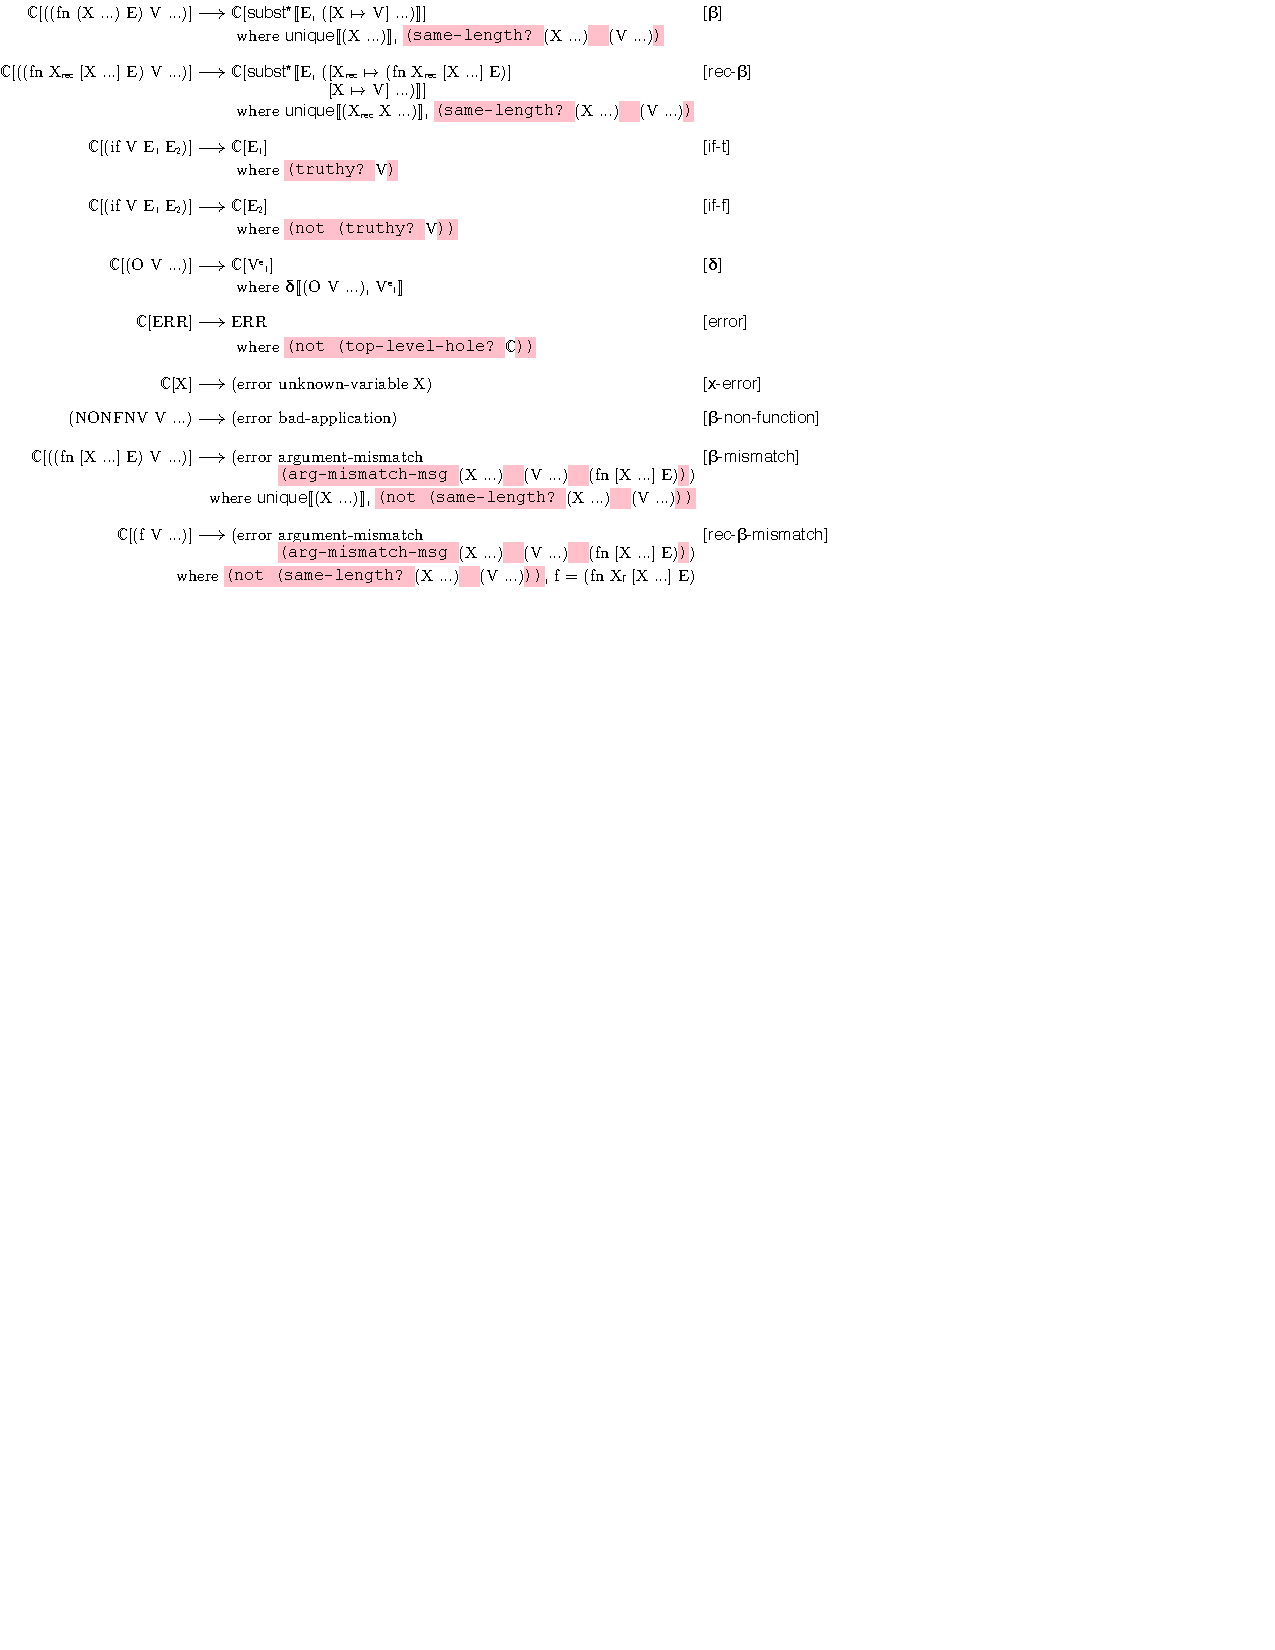
\includegraphics[]{redex/arrowv.pdf}
}
\caption{Small-step reduction relation in $\lambda c$.
  We define $\beta$ reduction rules for both types of functions.
  Then branching rules for conditionals (\texttt{false} and \texttt{nil} are false values),
  and constant functions ($\delta$, full definition omitted).
  Finally several rules for throwing detailed runtime errors.
  }
  \label{arrowv}
\end{figure}

\begin{figure*}
\fbox{
  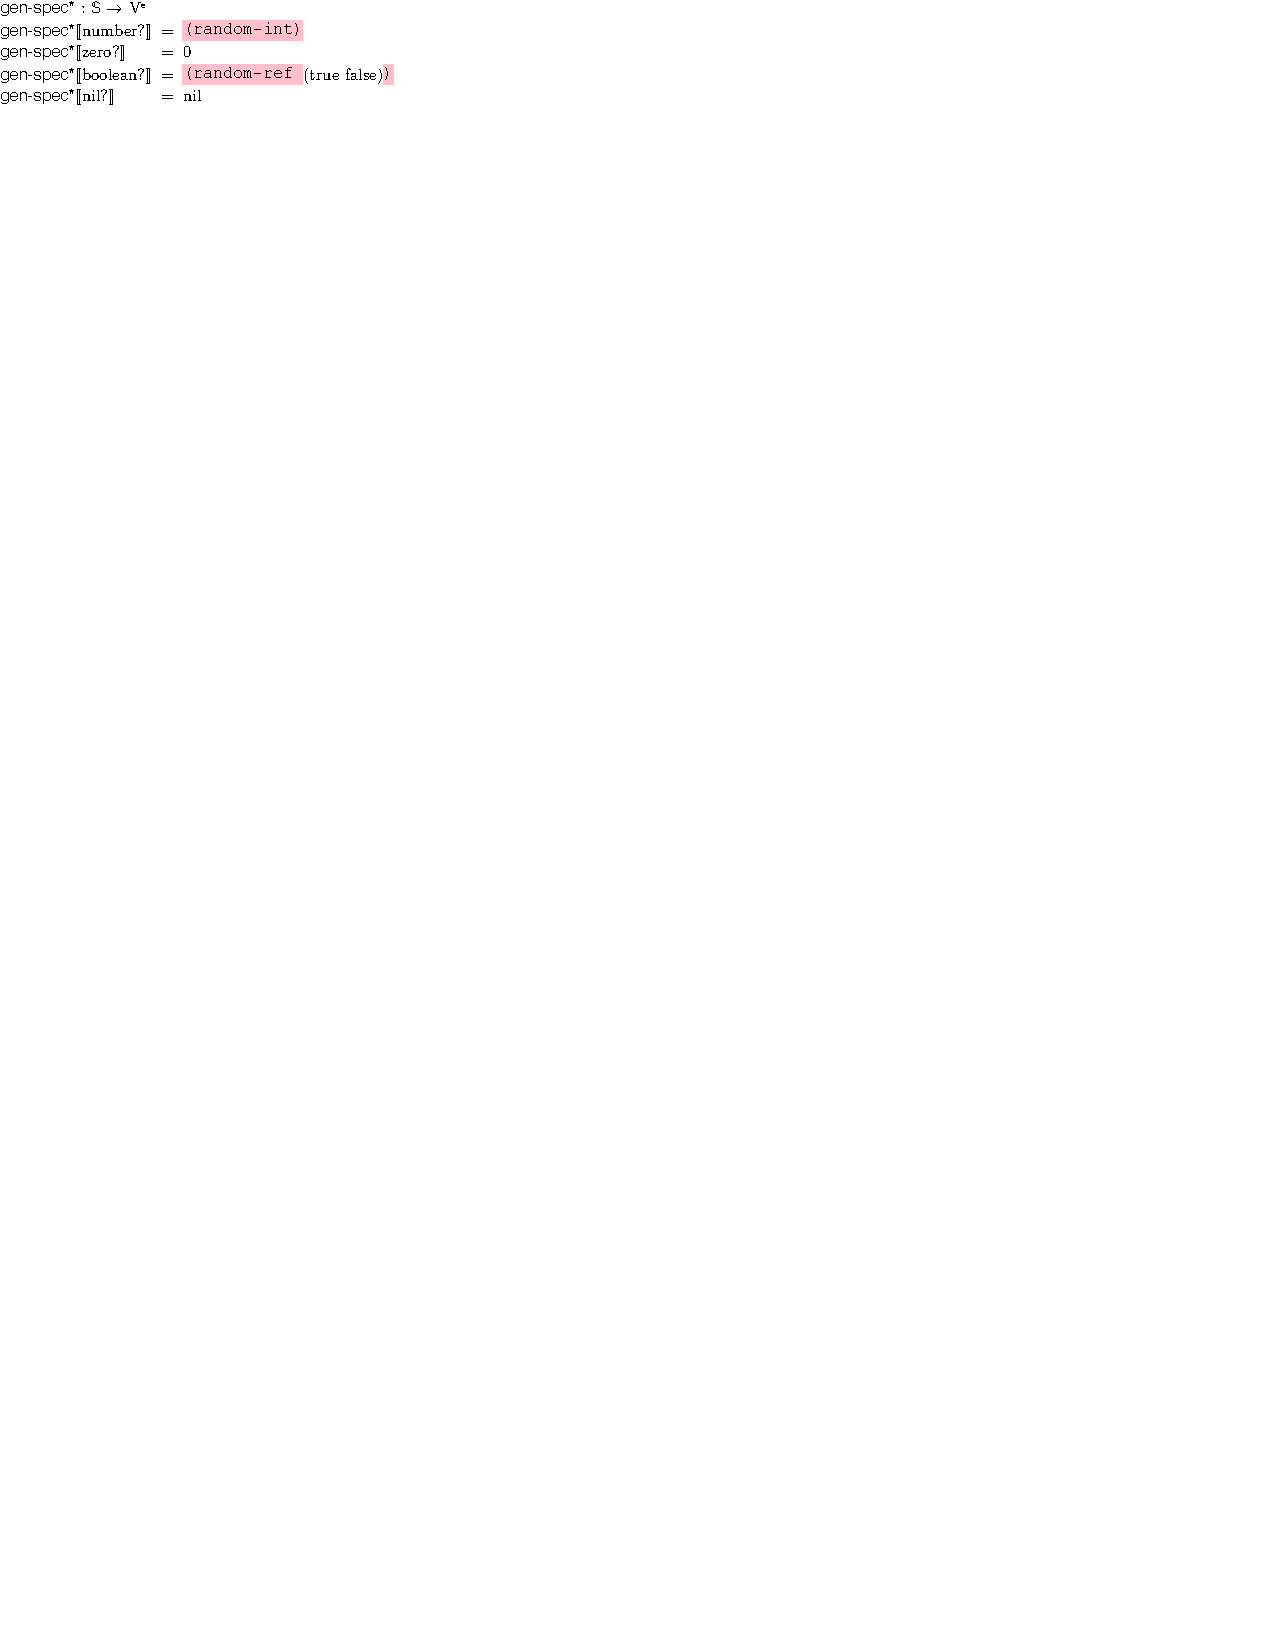
\includegraphics[]{redex/gen-spec*.pdf}
}

\fbox{
  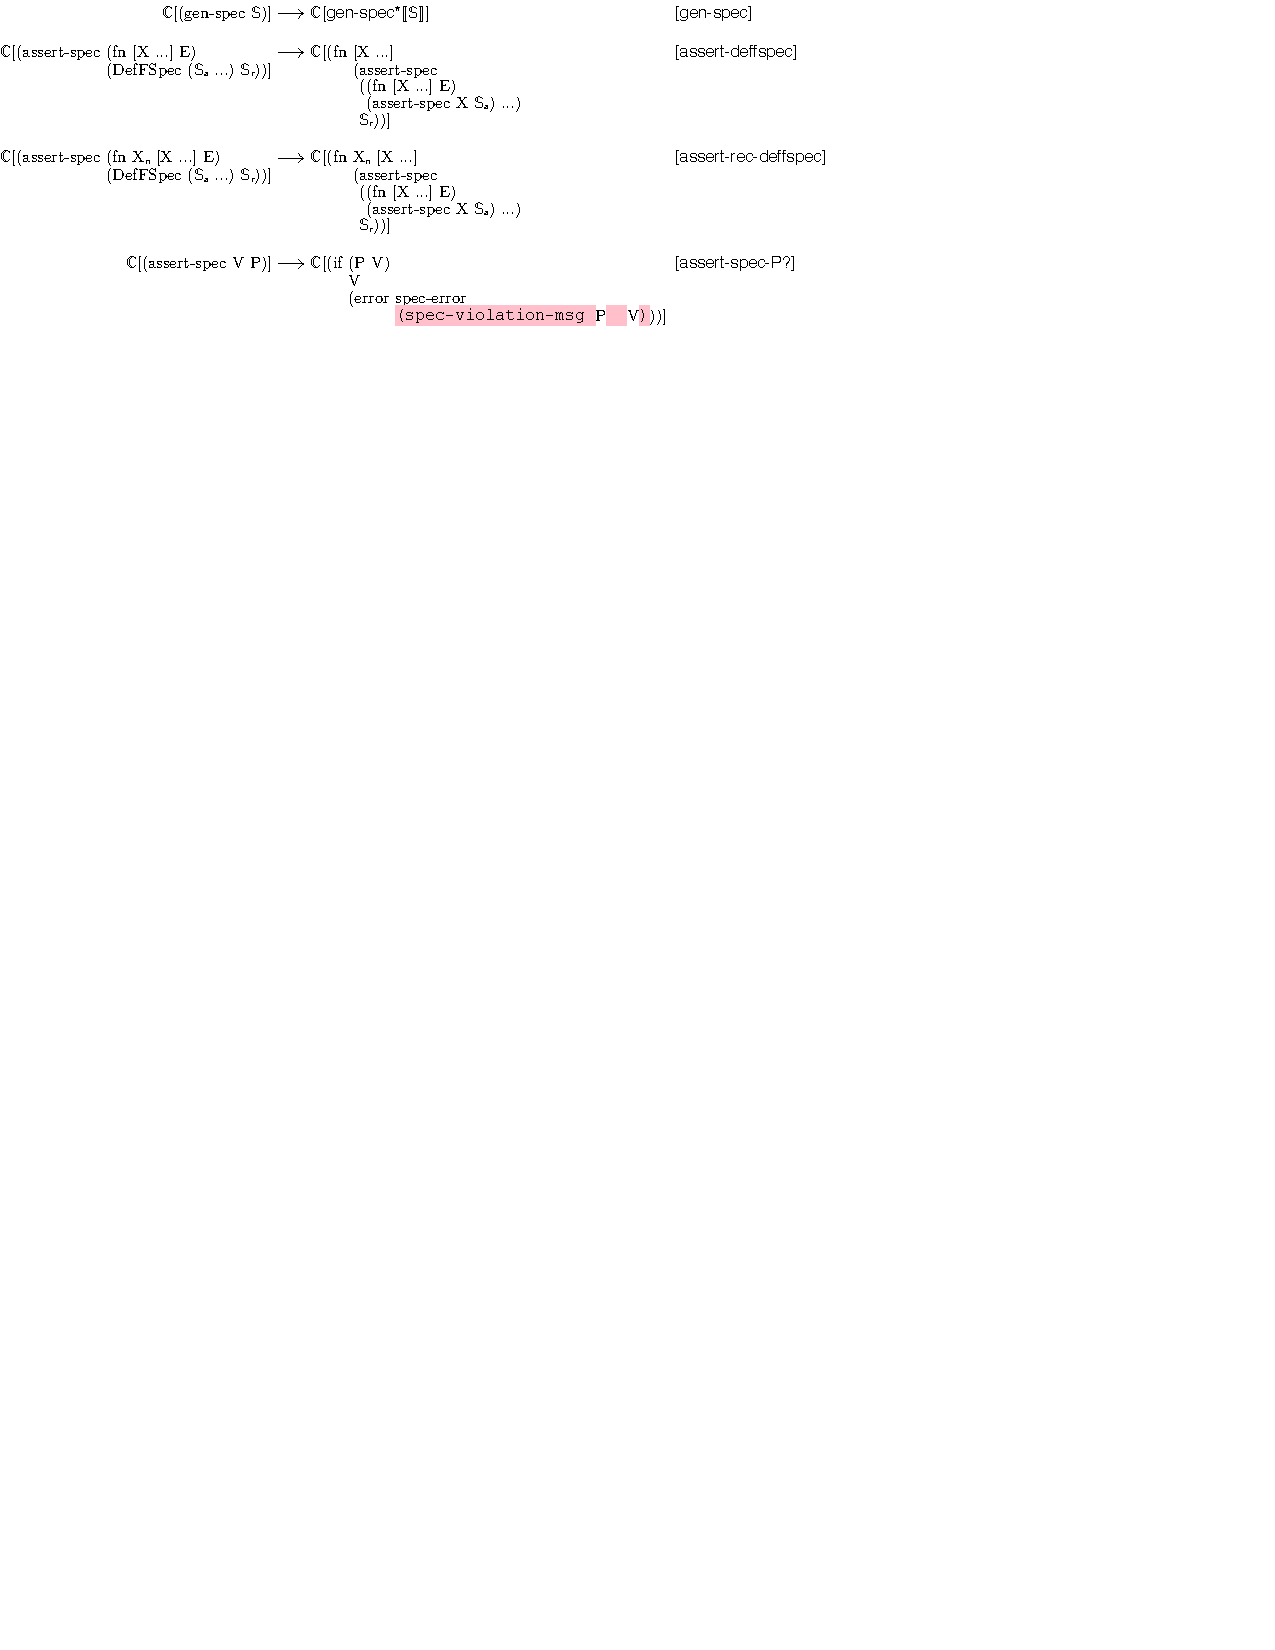
\includegraphics[]{redex/arrowvspec.pdf}
}
\caption{Small-step reduction relation in $\lambda c_s$ (extending $\lambda c$, Figure~\ref{arrowv}).
  \texttt{gen-spec} takes a spec and generates a value conforming to that spec
  via the \texttt{gen-spec*} metafunction.
  We define \texttt{assert-spec} with support for 
for \texttt{fdef} using traditional proxy checking semantics, and flat predicates.}
  \label{arrowvspec}
\end{figure*}

\begin{figure*}
\fbox{
  
\includegraphics[]{redex/gen-spec*-hof.pdf}
}

\fbox{
  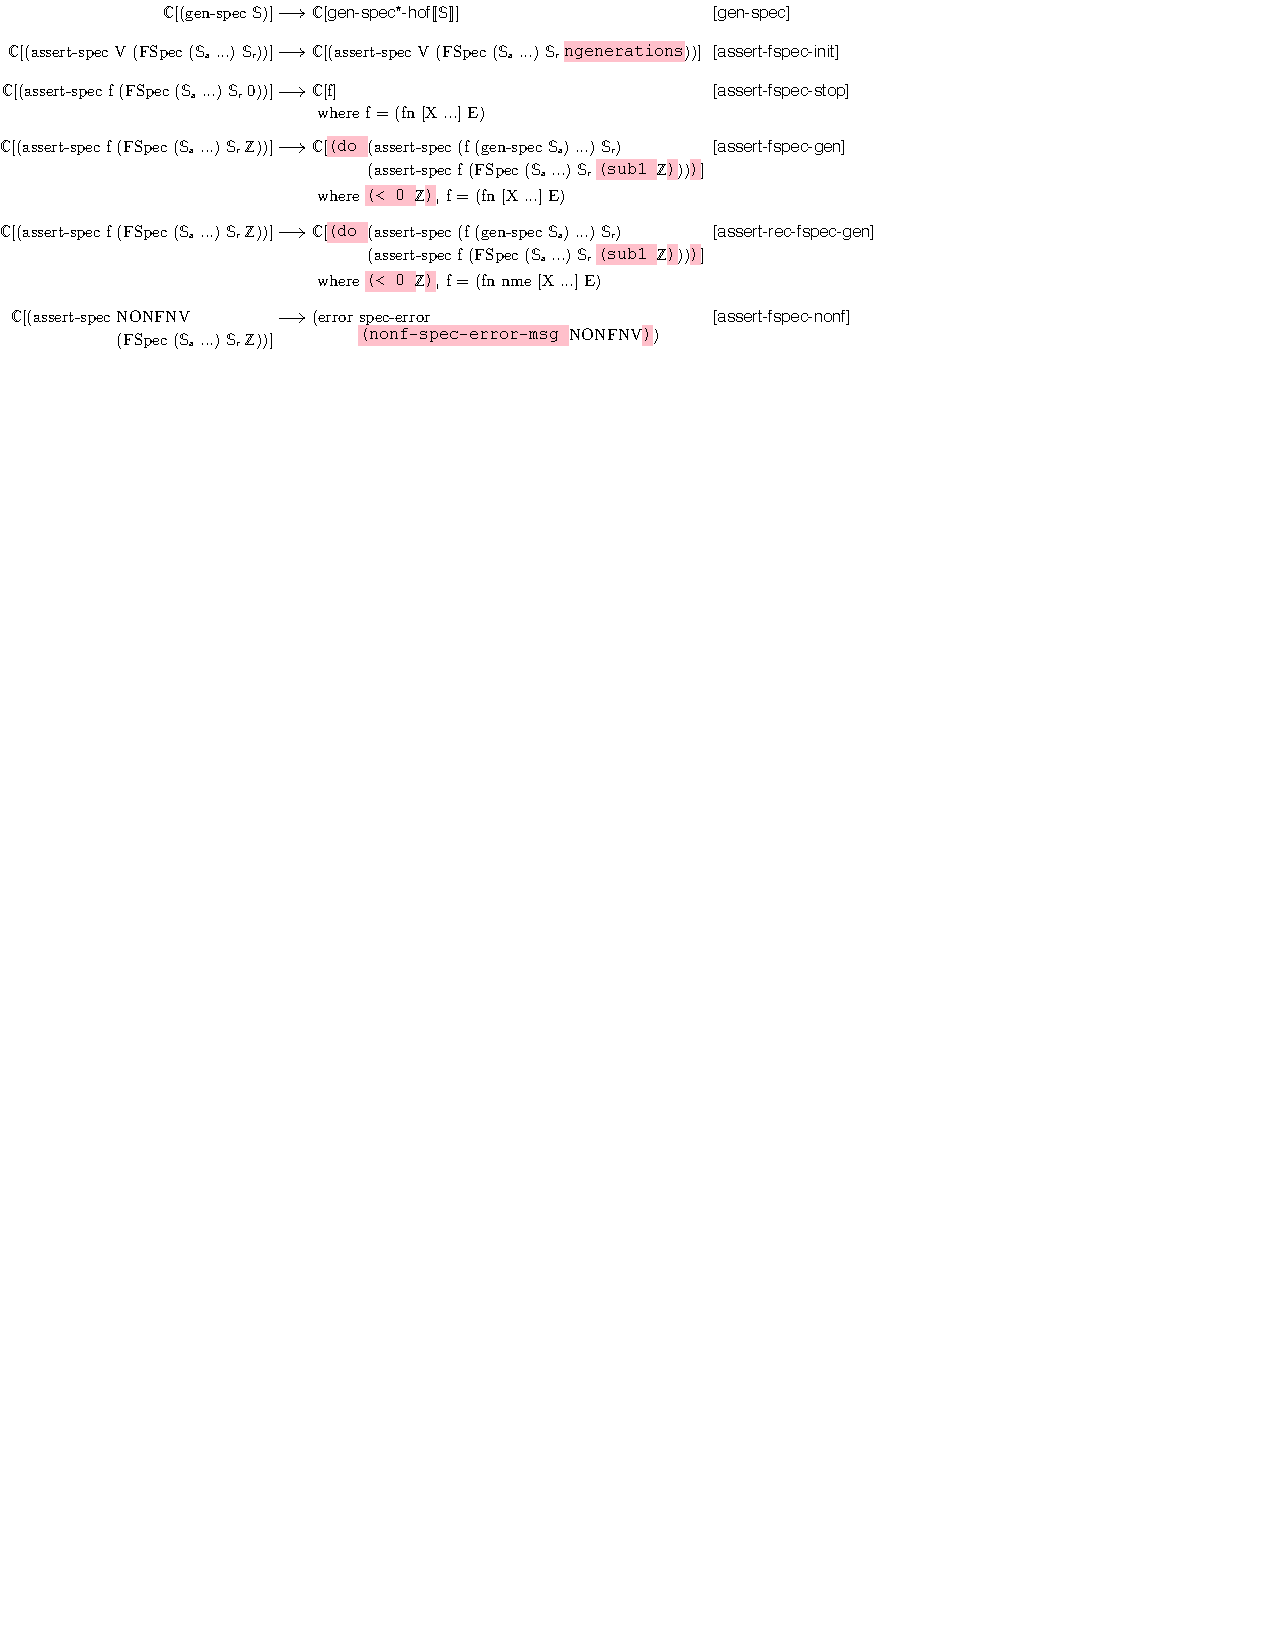
\includegraphics[]{redex/arrowvspec-hof.pdf}
}
  \caption{Small-step reduction relation for $\lambda c_{s}^{f}$ (extending $\lambda c_s$, Figure~\ref{arrowvspec})
  \texttt{gen-spec} takes a spec and generates a value conforming to that spec
  via the \texttt{gen-spec*-hof} metafunction (which extends \texttt{gen-spec*} in Figure~\ref{arrowvspec}).
	Since we add \texttt{fspec}s, \texttt{gen-spec*-hof} can generate values conforming to \texttt{fspec}s
(dummy functions that have the expected number of parameters, and generate their return values).
\texttt{assert-fspec-init} initializes \texttt{FSpec} with an initial number of generations.
\texttt{assert-fspec-gen}  and
\texttt{assert-fspec-stop} handle the actual generative testing, with 
\texttt{assert-rec-fspec-stop} supporting recursive functions.
Finally, \texttt{assert-fspec-nonf} handles non-function values that are expected to
conform to an \texttt{fspec}.
  }
  \label{arrowvspec-hof}
\end{figure*}


\part{Typed Clojure Implementations}
\label{part:implementations}
\chapter{Background}

Clojure is a dialect of Lisp, and so supports metaprogramming
via macros.
This immediately poses an interesting problem for Clojure
type systems: how do we check a macro call?
Ideally, we don't want to require special typing rules for each
macro, since that imposes additional burden on the programmer
to define special rules for their own macros.
On the other hand, sometimes its helpful to write custom rules
for customized error messages, or a higher-level specification
for a macro's usage.

In this part we explore several solutions to this problem,
from the standard approach of expanding macros to
primitive forms before checking, to more involved solutions
that allow extensible typing rules for each macro.

Several constraints guide us through our designs.
There is a question of soundness: does what we actually
check match up with the code being evaluated?
There is a natural tension between soundness and user extensibility.
Allowing custom rules for macros gives a kind of flexibility
that makes it hard to relate type checking semantics with
the running code---which is the whole idea behind a soundness result.
On the other hand, expanding code before checking ensures
we check the actual code being run.
In all of these cases, wrappers that communicate information
to the type system are needed, but they interact
with evaluated code differently.

We also consider the experience of using these solutions.
Error messages can be unrelated to the source problem
if pre-expanding code, but we may miss actual errors
by using a poorly written typing rule.
We are interested in the difficultly of extending each system,
including any additional annotation burden,
additional knowledge needed to manage evaluation semantics
in typing rules, and additional type system knowledge required
to write typing rules. Finally, we also consider implications
to type checking performance and amenability to iterative development.

The following chapters present several designs of Typed Clojure,
their extensibility stories, and general implementation concerns for
Clojure type system designers.

%{
%\singlespacing
%\begin{verbatim}
%- Problem
%  - Clojure is a Lisp with macros
%  - don't want to write typing rules for each macro
%    - don't want to burden users
%    - so we expand them before checking
%    - but sometimes it's really helpful to write custom rules
%- Possible solutions
%  - pre expansion
%  - interleaved analysis and evaluation
%- Constraints
%  - Soundness?
%    - tension between soundness and user extensibility
%  - advantages of pre-expanding
%    - can't have "wrong" expansion in pre-expanded code
%      - we check the actual expansion that gets wr
%  - wrapper macros needed in all of these systems
%\end{verbatim}
%}

\chapter{Expand before checking}

Typed Clojure's initial design was inspired by Typed Racket,
which checks Racket code by first expanding until it consists
of only primitives, and then checking using fixed rules for each
primitive.
This chapter goes into this design in more detail, starting
with our choice of analyzer and then how to handle extensibility.

\section{Upfront Analysis with \texttt{tools.analyzer}}

Instead of using Clojure's compiler to analyze code,
we opted to use \texttt{tools.analyzer}, a standalone nano-pass
analyzer providing an idiomatic map-based AST format providing
passes for hygienic transformations and Java reflection resolution.

%{
%\singlespacing
%\begin{verbatim}
%- Pros to expanding up front:
%  - Separation of concerns (expander does expansion)
%- Cons to expanding up front:
%  - Lose contextual information from unexpanded macros while type checking.
%  - Requires wrapper macros which pollute runtime expansions and
%    often require copying implementation details (brittle).
%\end{verbatim}
%}

\figref{fig:analyzer:control-flow-pre-expand} demonstrates 
how Typed Clojure checks code using the pre-expansion approach.
To simplify presentation we assume \texttt{tools.analyzer}
uses only 2 passes. The first pass \texttt{analyze} creates
a bare AST with no platform specific information.
The second pass is composed of two tree traversals.
The first is a pre-traversal \texttt{pre-passes} which
is called before we visit the children of an AST node.
The second is a post-traversal \texttt{post-passes} which
is called after we visit the children of an AST node.

This arrangement is convenient as a type system implementer,
insofar as there is a clean separation of concerns: the analyzer
handles expansion and evaluation, while the type system
merely checks.
However, much contextual information is lost from the expansion
process that is needed for checking.
We now present how we surmount this challenge while still
preserving the pre-expanded checking model.

\begin{figure}
\singlespacing
$$
  \begin{array}{r||l|l|l|}
    \text{Time} & \text{\clj{(let [...]}} & \text{\clj{(cond ...}} & \text{\clj{(+ ...)))}}\\
    \hline
     0          & \text{\clj{analyze}}^{>}    &                             &                      \\
     1          &                             & \text{\clj{analyze}}^{>}    &                      \\
     2          &                             &                             & \text{\clj{analyze}}^{>} \\
     3          &                             &                             & \text{\clj{analyze}}^{<} \\
     4          &                             & \text{\clj{analyze}}^{<}    &                      \\
     5          & \text{\clj{analyze}}^{<}    &                             &                      \\
     6          & \text{\clj{pre-passes}}^{>} &                             &                      \\
     7          &                             & \text{\clj{pre-passes}}^{>} &                      \\
     8          &                             &                             & \text{\clj{pre-passes}}^{>} \\
     9          &                             &                             & \text{\clj{post-passes}}^{<} \\
     10         &                             & \text{\clj{post-passes}}^{<}&                      \\
     11         & \text{\clj{post-passes}}^{<}&                             &                      \\
     12         & \text{\clj{check}}^{>}      &                             &                      \\
     13         &                             & \text{\clj{check}}^{>}      &                      \\
     14         &                             &                             & \text{\clj{check}}^{>} \\
     15         &                             &                             & \text{\clj{check}}^{<} \\
     16         &                             & \text{\clj{check}}^{<}      &                      \\
     17         & \text{\clj{check}}^{<}      &                             &                      \\
  \end{array}
$$
%\begin{verbatim}
%time | (let [...]  | (cond ...   | (+ ...)))
% |   | ---------------------------------------
% v   | analyze    >|             |
%     |             | analyze >   |
%     |             |             | analyze    >
%     |             |             |<analyze
%     |             |<analyze     |
%     |<analyze     |             |
%     | pre-passes >|             |
%     |             | pre-passes >|
%     |             |             | pre-passes >
%     |             |             |<post-passes
%     |             |<post-passes |
%     |<post-passes |             |
%     | check>      |             |
%     |             | check>      |
%     |             |             | check>
%     |             |             |<check
%     |             |<check       |
%     |<check       |             |
%\end{verbatim}
  \caption{Illustrative control flow when
  using \texttt{tools.analyzer} to expand code via \clj{analyze} and several passes,
  followed by Typed Clojure checking.
  The partial expression \clj{(let [...] (cond ... (+ ...)))}
  was chosen since it has at least 3 levels of nesting.
  Many more levels will be revealed after expansion by \clj{analyze}, which we do not picture.
  ${}^>$ and ${}^<$ indicate work done to a node before and after processing its children, respectively.
  }
  \label{fig:analyzer:control-flow-pre-expand}
\end{figure}

\section{Extensibility}

%{
%\singlespacing
%\begin{verbatim}
%- Problem
%  - need to communicate between type system and Clojure runtime
%- Constraints
%  - a "typed" program must evaluate unchanged via normal Clojure compilation
%    - extensions must be done via macros provided by Typed Clojure
%      - imported and used as normal by Clojure programmers
%    - in contrast to #lang system
%      - which always guarantees the type system is in charge of expanding
%      - (both approaches use macros for extension and to share information)
%- how to communicate to type system via expanded code?
%  - eg. tc-ignore, ann-form
%  - in Racket you would use syntax properties, or side effects
%  - Clojure has metadata, but not as robust as syntax properties
%    - how metadata is compiled is implementation dependent (I forgot how?)
%    - we decided to emit special `do` forms to communicate with type system
%      - (do :special-form ...)
%      - "variable protocol" in Advanced Macrology
%  - side effects
%    - Clojure's compilation strategy is straightforward
%      - files are just sequences of top-level forms
%      - evaluate each in turn
%      - side effects of expanding/evaluating a previous form
%        can be used to compile a subsequent form
%      - members of top-level `do` forms are also top-level forms, and thus
%        are evaluated in turn
%    - Typed Clojure collects global type annotations by evaluation side effects
%      - macroexpansion side effects not used in case AOT compiled
%- how to define custom rules?
%  - Approach 1: custom expansions for embedding typing rules in expansion
%  - Approach 2: "typing rules by analogy"
%    - lose ability to check actual expansion
%\end{verbatim}
%}

Now that we have outlined how we use \texttt{tools.analyzer} to pre-expand code before type checking,
we describe Typed Clojure's approach to sharing information between the programs it checks
and the type system.
We deviate significantly from Typed Racket's approach~\cite{Culpepper07advancedmacrology}
mostly because of differences in compilation models between Clojure and Racket.

One constraint we must consider in Typed Clojure is that a ``typed'' Clojure program must
evaluate unchanged under normal Clojure compilation. In Racket, we could instead specify
the language under which a module is compiled using the \texttt{\#lang} directive---this is Typed
Racket's approach. 
In Clojure, there is just one language and no built-in facilities to extend the compilation
process, so Typed Clojure provides a suite of macros for communicating with the type system that
users must explicitly load and use.

These macros come in several flavors:

\begin{itemize}
  \item syntax-based communication to type checker,
  \item side-effectful communication to type checker, and
  \item wrappers for existing untyped macros.
    %to avoid checking complex expansions
    %or provide .
\end{itemize}

We discuss each in the following sections.

\subsection{Syntax-based communication}

A simple macro provided by Typed Clojure that communicates to the checker
via syntax is \clj{tc-ignore}, which takes a number of forms, places
them in a \clj{do} form, and tells the checker to ignore the resulting
form and assign it type \clj{Any}.

\begin{figure*}
\begin{cljlisting}
(defmacro tc-ignore 
  "Ignore forms in body during type checking"
  [& body]
  `(do :clojure.core.typed.special-form/special-form
       :clojure.core.typed/tc-ignore
       ~@(or body [nil])))
\end{cljlisting}
  \caption{Public facing macro definition for \clj{tc-ignore}.}
  \label{fig:analyzer:tc-ignore}
\end{figure*}

\figref{fig:analyzer:tc-ignore} shows the implementation of the \clj{tc-ignore} macro.
It demonstrates the \clj{do}-special-form protocol:
if the first member of a \clj{do} is the keyword
\clj{:clojure.core.typed.special-form/special-form},
the following keyword names a special typing rule to use
to check the entire form.
A corresponding typing rule must then be registered with the type checker under this name,
like in \figref{fig:analyzer:tc-ignore-do-op}.

\begin{figure*}
\begin{cljlisting}
(defmethod internal-special-form :clojure.core.typed/tc-ignore
  [expr expected]
  (tc-ignore/check-tc-ignore check-expr expr expected))
\end{cljlisting}
  \caption{Registering a corresponding typing rule for \clj{tc-ignore} via the \clj{do}-special-form protocol.}
  \label{fig:analyzer:tc-ignore-do-op}
\end{figure*}

Clojure's compilation and runtime models make \clj{do} statements an excellent candidate for the basis of
an extensible syntax-based communication protocol.
First, it naturally inherits the top-level characteristics of \clj{do}, which is key to defining
wrapper macros that operate at the top-level.
A usage of \clj{tc-ignore} that relies on this is demonstrated in \figref{fig:analyzer:tc-ignore-usage}.
Second, it avoids the need to pre-expand its arguments to attach information, or
have special cases for particular arguments.
On the other hand, a communication protocol based on attaching metadata properties
would require pre-expanding arguments, since metadata is lost on macroexpansion,
and in some cases would not be possible, since many common Clojure forms do not support metadata
(such as keywords, numbers, and nil).
Third, the information can be compiled away using standard techniques,
since they are constant statements---extra information can be provided via a map of constant values
placed after the typing rule name, as in
the definition of \clj{ann-form} (\figref{fig:analyzer:ann-form-definition}).

\begin{figure*}
\begin{cljlisting}
(defmacro ann-form
  "Annotate a form with an expected type."
  [form ty]
  `(do :clojure.core.typed.special-form/special-form
       :clojure.core.typed/ann-form
       {:type '~ty}
       ~form))
\end{cljlisting}
  \caption{The definition of \clj{ann-form} shows how to communicate extra information to the type checker}
  \label{fig:analyzer:ann-form-definition}
\end{figure*}

While a strong choice, there are some downsides to basing our communication protocol on \clj{do}
statements.
There is no guarantee the information will be compiled away at runtime, and
thus may contribute to bloating the runtime.
On the other hand, \clj{tools.analyzer} must be carefully configured to not erase these constant
values before Typed Clojure can access them.

Alternative \clj{do}-based protocols could be similarly effective
such as attaching metadata directly to the symbol \clj{do} or list \clj{(do ...)}.
We felt embedding the information directly in programs had the best chance of forward-compatibility,
since the interaction between metadata and compilation is not well documented and
can be platform-dependent (in our experience ClojureScript has handled some cases differently,
like evaluating metadata instead of simply quoting it as in Clojure).

\begin{figure}
\begin{cljlisting}
(tc-ignore
  (defmacro reverse-app [a f] `(~f ~a))
  (reverse-app 1 inc)) ;=> 2
\end{cljlisting}
  \caption{Example top-level usage of \clj{tc-ignore}
           where the second form must expand after the first evaluates.
  It works because \clj{tc-ignore} wraps only with \clj{do}.}
  \label{fig:analyzer:tc-ignore-usage}
\end{figure}

\subsection{Side-effectful communication}

Racket has a sophisticated system for managing compile-time side effects
to accompany its module system.
Clojure does not have a module system, and instead relies on conventions
and a simple compilation model to write effective programs.

The unit of compilation in Clojure is a top-level form. A top-level Clojure form
is guaranteed to have all previous top-level forms fully expanded
and evaluated before it is expanded and evaluated itself.
This blurs the lines between compile-time and runtime, compared to the
distinct phases of Racket compilation.

When checking a file with Typed Clojure, we have similar guarantees:
when checking a top-level form, we can depend on the fact that all
previous top-level forms have been expanded, evaluated, and checked,
and that the current form has been fully expanded.

Thus, we have a choice of (at least) three times to send side-effectful communication
to the type checker:
expansion-time, evaluation-time, and checking-time.
\figref{fig:analyzer:ann-definition} shows the most frequently used
side-effectful macro \clj{ann}, which registers the type of a var in the
global environment.
It expands to code that uses internal function \clj{ann*}, which does
the registering. This is a \emph{evaluation-time} side effect,
and we similarly perform most communication at this time.
We now elaborate on why this is a good choice.

A previous implementation of Typed Clojure (which was used by CircleCI
in \secref{sec:casestudy}) only collected top-level annotations
from \clj{ann} at checking-time. This forced Typed Clojure to recursively
check other files just to collection annotations.
We decided the natural behavior of rechecking a file would be to
recheck its dependencies so, among other benefits, top-level annotations
would be kept up-to-date.
Unfortunately, the checker was much slower at evaluating files
than the Clojure compiler, meaning iterative development was hampered.
To fix this, we made checking of transitive file dependencies optional, and
so dependencies containing top-level annotations would potentially only 
be evaluated by the Clojure compiler.
Evaluation-time was then the natural time to collect these annotations.

A side-effect of this design choice is that it is no longer a sound idea to
infer types for unannotated top-level bindings. In the aforementioned 
implementation, if the checker finds an unannotated top-level \clj{def}
like \clj{(def a 1)}, it will update the global environment with the 
inferred type of the right-hand-side.
Now that transitive dependencies are optionally checked, it is not guaranteed
the checker will infer these annotations, and so more top-level annotations
via \clj{ann} are needed to recover consistent checking behavior.
This unfortunately increases the annotation burden even more, however the rewards
are great.
We believe that Clojure programmers will enjoy the ability to rapidly recheck
small parts of their code base, just like they are used to in untyped Clojure.

Now, we discuss the merits of collection at evaluation-time over expansion-time.
We avoid expansion-time for side-effects because Clojure code can be
evaluated in two ways: from the original source code in interpreted mode, and 
from precompiled JVM bytecode in ahead-of-time compilation mode.
In the latter, code is expanded ahead-of-time (potentially in a different environment)
and thus expansion-time side-effects are lost.
We applied the standard solution to this problem: remove the side-effect from
the macro itself and move it to the evaluation of the code it expands into.


%\begin{verbatim}
%- not forced to recursively check other files just to collect annotations
%  - problem identified with CircleCI
%  - simply need to evaluate a file normally
%  - in turn requires more annotations
%    - tradeof between annotation burden and performance
%- avoid relying on expansion-time side effects
%  - lost with AOT compilation
%- "staged at checking time": under Typed Racket AOT compilation, it stages global type annotations for eval time
%  - we don't have a similar mode
%    - compiling a Typed Clojure file does not require checking
%\end{verbatim}


\begin{figure*}
\begin{cljlisting}
(defmacro ann 
  "Register top-level var with type."
  [varsym typesyn]
  (let [qsym (qualify-in-current-ns varsym)
        opts (meta varsym)
        check? (not (:no-check opts))]
    `(tc-ignore (ann* '~qsym '~typesyn '~check? '~&form))))
(defn ann* 
  "Internal use only. Use ann."
  [qsym typesyn check? form]
  ; omitted - registers `qsym` at type `typesym`
  )
\end{cljlisting}
  \caption{Implementation of \clj{ann}, which expands to code that registers types at evaluation-time.}
  \label{fig:analyzer:ann-definition}
\end{figure*}

\subsection{Wrapper macros}

Several situations call for wrapper macros for existing untyped macros.
In practice, this often means the type system author provides an alternative
implementation for a macro, and the type system user
replaces any usages of the original macro in type-checked code with the alternative implementation.
Sometimes this choice is aesthetic, providing a prettier 
way to write annotations. For example, the \clj{fn} wrapper
enables writing annotations like
\clj{(fn [a :- Int] ...)}
instead of the more verbose
\clj{(ann-form (fn [a] ...) [Int -> Any])}.

The more pressing need for wrapper macros when checking pre-expanded
code is to manage complex expansions.
Some macro expansions are too complex for Typed Clojure to reason about,
so it becomes necessary to rewrite these expansions to be more palatable
for the checker.
For example, the \clj{for} macro is a lazy sequence builder using
a list-comprehension syntax---however it expands into local
loops using local mutable state, which are problematic to check.
The wrapper macro for \clj{for} expands (and thus evaluates) similarly, but inserts user-provided
type annotations strategically into the expansion so it more easily type checks.

The problem with this kind of wrapper macros is that large amounts
of implementation code must be copied to preserve the original semantics.
Instead of checking a higher-level specification of the macro's behavior,
we are tied closely to a particular implementation.
This has the advantage of checking the actual code that gets evaluated, but
unfortunately
requires the type system writer to closely follow the original implementations
(hampering both backwards- and forwards-compatibility with versions of the original macro).
Furthermore, users not only must use wrapper macros where necessary, but
also recognize when they are required---usually attempting to check a complex
expansion yields an incomprehensible error as Typed Clojure fails to check it.
It is rarely apparent that a wrapper macro is needed from such an error message.

\chapter{Interleaved expansion and checking}

The previous chapter outlined a design for Typed Clojure that fully expands code
before checking.
We identified several problems with the user experience of Typed Clojure's initial design,
including bad error messages, and excessive copying of macro implementations for wrapper
macros.
Additionally, we identified several issues with \texttt{tools.analyzer} that we have
not yet discussed.

First, \texttt{tools.analyzer}'s goals of being mostly platform-agnostic made analysis particularly 
slow, and so added an undesirable performance overhead to type checking.
In particular, a copy of the
global scope is maintained for every namespace. While it enables a convenient platform-agnostic API
for symbol resolution,
it comes at a performance cost since it must be updated (from scratch) frequently.
Furthermore, some macroexpansion side effects are not (yet) recognized by the analyzer
which means analysis sometimes deviates from Clojure compiler, an undesirable situation
since Typed Clojure intends to model how code runs \emph{outside} of type checking.
Unfortunately, fixing some of these differences would require even more frequent costly updates.

Second, it is impractical to recover contextual information lost via analysis.
This is both because \texttt{tools.analyzer} has no way of representing unanalyzed
code (so there is no choice but to expand immediately), and
because \texttt{tools.analyzer} uses at least 2 passes over the AST
(so there is no obvious place to recover contextual information since pre-traversal
passes run \emph{after} the entire program has been expanded).
For example, \figref{fig:analyzer:control-flow-pre-expand}
illustrates \texttt{tools.analyzer}'s control flow with just 2 traversals.
Say at time 1 we wished to take advantage of the unexpanded \clj{cond}
form with a special rule (before it expands and contextual information is lost).
In fact, \texttt{tools.analyzer} provides the extension point \clj{macroexpand-1}
for just this purpose, which allows the user to specify exactly how a form is expanded.
Unfortunately, time 0 introduced local bindings that are unhygienic, and the hygienic
transformation pass (required for checking because occurrence typing's propositions do not recognize variable shadowing)
happens at time 6 with \clj{pre-passes}.
So, there is no room for a checking rule for \clj{cond} until time 13, well
after the \clj{cond} is expanded away.

Fortunately, \texttt{tools.analyzer}'s design and implementation
is otherwise brilliant and innovative, and forms a great base to build a new Clojure analyzer better suited to help solve
many of the aforementioned analysis and checking problems---we did exactly that in \texttt{core.typed.analyzer}.

\section{Interleaved Analysis with \texttt{core.typed.analyzer}}

To replace \texttt{tools.analyzer}, we built \texttt{core.typed.analyzer}. In this section,
we describe how \texttt{core.typed.analyzer} works, and outline both the ideas we repurposed
from \texttt{tools.analyzer} and those specific to \texttt{core.typed.analyzer}.

\subsection{Overview}

The main feature of \texttt{core.typed.analyzer} is the ability to stop and resume
analysis at any point, while still supporting the essentials of a general-purpose Clojure analyzer.
Supporting this requires several key innovations and restrictions over \texttt{tools.analyzer}.
First, a new AST node type for partially expanded forms is needed to return a paused analysis.
Second, the analyzer must have the ability to incrementally perform a small amount of analysis
(on the order of expanding one macro) to provide fine-grained control over the AST.
Third, all AST traversals must be fused into one traversal to minimize
the bookkeeping needed to manage the AST.

To this end, \texttt{core.typed.analyzer} provides an API of 4 functions.
First, \clj{(unanalyzed form env)} creates an \clj{:unanalyzed} AST node
that pauses the analysis of \clj{form} in local environment \clj{env}.
Second, \clj{(analyze-outer ast)} analyzes the outermost form represented by \clj{ast}
further by roughly one macroexpansion if possible, otherwise it returns \clj{ast}.
Third, \clj{(run-pre-passes ast)} and \clj{(run-post-passes ast)}
decorate \clj{ast} with extra information, used before and after visiting its children,
respectively.

To sample how it feels to use this API to implement a type checker, we now
walk through checking \clj{(let [...] (cond ... (+ ...)))} in \figref{fig:analyzer:typed-analyzer-overview}.
To check the outermost \clj{let},
we use \clj{unanalyzed} to create an initial AST from a entire form at time 0.
Then at time 1, the checker calls \clj{analyze-outer} zero or more times, either 
until a special rule for partially expanded code is triggered
or to a fixed point.
Next at time 2 and 3 we decorate our AST node with \clj{run-pre-passes} (adding hygienic bindings)
before calling \clj{check}.
After checking its children during time 4-13, at time 14 and 15 we use \clj{run-post-passes}
to add the rest of the decorations (e.g., resolving interop reflection)
before any final checks from \clj{check}.
The interleaving of operations using \texttt{core.typed.analyzer} is clear to see when
compared to the same example using \texttt{tools.analyzer} 
(\figref{fig:analyzer:control-flow-pre-expand}).

Now with the interleaving analyzer, we can solve the problem we posed at the beginning of this chapter
of wanting a custom typing rule for \clj{cond}: we simply
limit the number of expansions done via \clj{analyze-outer} at time 4 
before calling \clj{check} (\figref{fig:analyzer:typed-analyzer-overview}).
The call to \clj{run-pre-passes} at time 2 will make any introduced let bindings hygienic,
and so it's safe to reason about them with occurrence typing, and thus Typed Clojure.


\begin{figure*}
\singlespacing
$$
  \begin{array}{r||l|l|l|}
    \text{Time} & \text{\clj{(let [...]}}            & \text{\clj{(cond ...}}          & \text{\clj{(+ ...)))}}          \\
    \hline
     0          & \text{\clj{unanalyzed}}^{>}        &                                 &                                 \\
     1          & \text{\clj{analyze-outer}}^{*}     &                                 &                                 \\
     2          & \text{\clj{run-pre-passes}}^{>}    &                                 &                                 \\
     3          & \text{\clj{check}}^{>}             &                                 &                                 \\
     4          &                                    & \text{\clj{analyze-outer}}^{*}  &                                 \\
     5          &                                    & \text{\clj{run-pre-passes}}^{>} &                                 \\
     6          &                                    & \text{\clj{check}}^{>}          &                                 \\
     7          &                                    &                                 & \text{\clj{analyze-outer}}^{*}  \\
     8          &                                    &                                 & \text{\clj{run-pre-passes}}^{>} \\
     9          &                                    &                                 & \text{\clj{check}}^{>}          \\
     10         &                                    &                                 & \text{\clj{run-post-passes}}^{<}\\
     11         &                                    &                                 & \text{\clj{check}}^{<}          \\
     12         &                                    & \text{\clj{run-post-passes}}^{<}&                                 \\
     13         &                                    & \text{\clj{check}}^{<}          &                                 \\
     14         & \text{\clj{run-post-passes}}^{<}   &                                 &                                 \\
     15         & \text{\clj{check}}^{<}             &                                 &                                 \\
  \end{array}
$$

  \caption{Illustrative control flow for interleaved checking and analysis using
  \texttt{core.typed.analyzer}. ${}^*$ denotes zero or more calls.
  }
  \label{fig:analyzer:typed-analyzer-overview}
\end{figure*}

\subsection{Implementation}

Passes in \texttt{tools.analyzer} are written completely separately and connected to other passes
via explicit dependencies specified via metadata.
This allows a separate scheduler to arrange the passes into as few tree traversals as possible,
and means passes are highly modular, so we can choose just those that are relevant to type systems.
Furthermore, passes are almost always extensible via Clojure's multimethods, so it is trivial to add
support for new AST types, like an AST representation for unanalyzed code.

% - resolve-sym is platform dependent, etc.

\begin{figure}
\begin{cljlisting}
(defn unanalyzed
  "Create an unanalyzed AST node from form and env"
  [form env]
  {:op :unanalyzed
   :form form
   :env env
   ;; ::config will be inherited by whatever node
   ;; this :unanalyzed node becomes when analyzed
   ::config {}})
\end{cljlisting}
  \caption{Constructor for unanalyzed nodes.}
  \label{fig:analyzer:unanalyzed-ctor}
\end{figure}

\begin{cljlisting}
(defn check-expr
  "Check an AST node has the expected type."
  [expr expected]
  (if (= :unanalyzed (:op expr))
    (check-expr (analyze-outer expr) expected)
    (run-post-passes
      (check (run-pre-passes expr)
             expected))))
(defn check-form
  "Check a Clojure expression has the expected type"
  [form expected]
  (check-expr (unanalyzed form (empty-env))
              expected))
\end{cljlisting}

%{
%\singlespacing
%\begin{verbatim}
%- Goals
%  1. Build a better tools.analyzer
%     - too slow
%     - too many passes
%     - reuse the passes/scheduler/analysis
%       - and :unanalyzed
%         - instead of analyzing children, store context and return
%       - unforce one pass
%  2. Extensibility
%     - we want custom rules for syntax BEFORE expansion
%     - avoid need for wrapper macros
%       - avoid implementation-dependence
%       - better error messages for users
%     - but lose ability to check actual expansions
%- (This is the Turnstile approach)
%  - Except we don't have syntax objects, how to do it?
%- Create a single-pass tools.analyzer variant that can be paused in
%  the middle of analysis
%  - `analyze` now expands absolute minimum (usually 1 macro)
%- now `check` has access to the raw Clojure forms before they are expanded
%  - much power = much reponsibility
%    - top-level evaluation side effects
%    - expansion side effects
%      - talk about that in a different chapter
%    - must manually manage local scope
%    - avoiding double macro expansion
%    - avoiding double evaluation
%    - double analysis is OK though, no side effects
%      - so we can "reinsert" a fully analyzed AST back into
%        a macro call so it can be expanded as usual.
%        - eg. (my-macro (unexpanded))
%            =>
%              (my-macro ~(check (unexpanded) ...))
%- Pros
%  - now have access to original macro forms for higher-level reasoning
%- Cons
%  - no longer checking the implementation of macros
%    - although were we ever, really?
%      - wrapper macros are copied implementation details
%  - must carefully manage compile-time side effects
%\end{verbatim}
%}


\begin{figure*}
\begin{cljlisting}
; tools.analyzer version
(defn parse-if
  "Convert a Clojure `(if <test> <then> <else>)` form to an AST."
  [[_ test then else :as form] env]
  {:op      :if
   :form     form
   :env      env
   :test     (__red>analyze-form<red__ test (assoc env :context :ctx/expr))
   :then     (__red>analyze-form<red__ then env)
   :else     (__red>analyze-form<red__ else env)
   :children [:test :then :else]})

; core.typed.analyzer version
(defn parse-if
  "Convert a Clojure `(if <test> <then> <else>)` form to an AST."
  [[_ test then else :as form] env]
  {:op      :if
   :form     form
   :env      env
   :test     (__red>unanalyzed<red__ test (assoc env :context :ctx/expr))
   :then     (__red>unanalyzed<red__ then env)
   :else     (__red>unanalyzed<red__ else env)
   :children [:test :then :else]})
\end{cljlisting}

  \caption{Example of porting a \texttt{tools.analyzer} function
  to use \clj{unanalyzed} (differences highlighted).
  }
\end{figure*}

\section{Extensibility in Interleaved checking}

\chapter{Managing Analysis Side effects}

{
\singlespacing
\begin{verbatim}
- introduce Clojure's evaluation model
  - `do` children treated as top-level
    - eg. (do e1 e2)
      - e1 is completely expanded+evaluated before e2 is expanded.
      - e2 can depend on evaluation-time side effects of e1
    - eg. (let [] (do e1 e2))
      - e1 is ONLY expanded before e2
      - e2 cannot depend on evaluation-time side effects of e1
- introduce *ns*, global thread-local variable that holds the current namespace
  - probably the most important evaluation-time side effect
    - changing namespaces
- introduce AOT-compilation
  - macroexpansions are performed upfront
    - so relying on expansion side-effects are uncommon and unreliable
- since checking & evaluation are interleaved, important that
  order-of-checking == order-of-evaluation
- but what about order-of-macroexpansion?
  - unaware of examples where order of macroexpansion side-effects are important
    outside of top-level forms
    - we have serious problems otherwise for any analysis tool
      - eg. (fn [] (change-ns-at-mexpansion-time) (relys-on-previous-macro-to-resolve))
        - this evaluates just fine in Clojure since there is
          no special handling of *ns* and things never pause and always just happen
          in order
        - but seems intractable for things like typing rules
          - custom typing rules must check forms in the order they are mexpanded!
            - seems very restrictive and error prone.
          - eg. ((fn [] ...) args ...)
            - imagine delaying checking a `fn` before its arguments.
              - but if args depend on fn body to expand, then we are forced
                to fully expand (ie. CHECK) the fn before checking the args.
                - very restrictive
- Relevant reading:
  - Flatt, "You want it, when?"
  - SamTH, Scheme 2007 (good for lispy background), PLDI 2011 (general audience)
\end{verbatim}
}

\begin{figure*}
\singlespacing
\begin{verbatim}
time | (do          | (defn a ...)| (defn b ...))
 |   | ----------------------------------------
 v   | analyze+eval>|             |
     | analyze     >|             |
     | pre-passes  >|             |
     |              | analyze >   |
     |              |<analyze     |
     |              | pre-passes >|
     |              |<post-passes |
     |              | check>      |
     |              |<check       |
     |              | eval  >     |
     |              |<eval        |
     |<analyze+eval |             |
     | analyze+eval>|             |
     |              |             | analyze >   
     |              |             |<analyze     
     |              |             | pre-passes >
     |              |             |<post-passes 
     |              |             | check>      
     |              |             |<check       
     |              |             | eval >
     |              |             |<eval
     |<post-passes  |             |
     |<analyze+eval |             |
\end{verbatim}
  \caption{}
  \label{fig:analyzer:control-flow-pre-expand-side-effects}
\end{figure*}

\begin{figure*}
\singlespacing
\begin{verbatim}
time | (do         | (defn a ...)| (defn b ...))
 |   | ---------------------------------------
 v   | check-tplvl |             |
     | analyze     |             |
     | pre-passes  |             |
     | check-child>|             |
     |             | analyze     |
     |             | pre-passes  |
     |             | check       |
     |             | post-passes |
     |             | eval        |
     | check-child<|             |
     |             |             | analyze
     |             |             | pre-passes >
     |             |             | check
     |             |             | post-passes
     |             |             | eval
     | post-passes |             |
\end{verbatim}
  \caption{}
  \label{fig:analyzer:control-flow-incremental-side-effects}
\end{figure*}


\part{Local Type Argument Synthesis with Symbolic Closures}

\chapter{Background}

As is inevitable for an optional type system, there are many
Clojure programs that Typed Clojure was not designed to type check.
These programs contain Clojure idioms that are often either intentionally
not supported by Typed Clojure's initial design, or 
were introduced to Clojure at a later date.
Regardless, programmers will inevitably want to use these features 
in their Typed Clojure programs---but crucially without breaking
support for existing idioms.
In this part, we explore what kinds of idioms are missing
support in Typed Clojure, and propose solutions in the form of
backwards-compatible extensions.

As we discussed in \partref{part:types}, Typed Clojure's initial
design is strongly influenced by Typed Racket. In particular,
Typed Clojure's static semantics of
combinining local type inference and occurrence typing
to check fully-expanded code
comes directly from Typed Racket.
This shared base is appropriate, given the similarities between
the base Clojure and Racket languages.
It is also effective, seamlessly handling many control flow
idioms, capturing many polymorphic idioms, and often yielding
predictable type error messages.
However, there are important tradeoffs to consider in this design---in the following
sections we introduce them and propose extensions to attempt to nullify
their downsides.

\section{Enhancing Local Type Inference}

``Local Type Inference''~\cite{PierceLTI} refers to the combination of
bidirectional type propagation 
specific approach
to partial type inference for languages with subtyping and impredicative
polymorphism.
``Partial type inference'' here is
problem of inferring 
(Pfenning~\cite{Pfenning1988partial} describes the distinction more thoroughly).

Concerning the limitations of local type inference,
Hosoya and Pierce~\cite{hosoya1999good}
isolate two drawbacks.
The first is dealing with ``hard-to-synthesize arguments''.
To understand this, we must appreciate a key ingredient of local type inference
called \emph{bidirectional propagation}, which 
we use the example of type checking \clj{(inc 42)} to demonstrate.
If we have already checked \clj{inc} to have type \clj{[Int -> Int]}, we
now have a choice of how to check the argument \clj{42} is an \clj{Int}.
The first is to ascribe an expected type to \clj{42} of \clj{Int}
and rely on
bidirectional \emph{checking mode} to ensure \clj{42} has the correct type
once we check it.
The second is to infer the type of \clj{42} (without an expected type) using 
bidirectional \emph{synthesis mode}, and then ensure the inferred type
is compatible with \clj{Int} after the fact.
A useful analogy in terms of expressions is that checking mode propagates
information outside-in, and synthesis mode propagates inside-out.
A similar analogy in terms of a type derivation tree (that grows upwards)
relates checking and synthesis modes to information being passed
up and down the tree, respectively.

To best serve the purposes of local type inference, it is crucial to stay in
bidirectional \emph{checking} mode as much as possible.
The ``hard-to-synthesize arguments'' problem occurs when type argument
inference interferes with the ability to stay in checking mode, and
thus forces the bidirectional propagator into synthesis mode
for arguments that require checking mode.
For example, to type check

\clj{(map (fn [x] (inc x)) [1 2 3])},

where \clj{map} has type

\clj{(All [a b] [[a -> b] (Seqable a) -> (Seqable b)])},

we use type argument inference to determine how to instantiate type variables \clj{a}
and \clj{b} based on \clj{map}'s arguments.
Unfortunately, 
to answer this question,
the naive local type inference algorithm~\cite{PierceLTI}
uses synthesis mode to retrieve the argument types,
and so checks \clj{(fn [x] (inc x))} in synthesis mode.
No information is propagated about the type of \clj{x},
so this expression will fail to type check, demonstrating
why functions are hard-to-synthesize.

The second drawback noted by Hosoya and Pierce are
cases where there is no ``best'' type argument to infer.
This occurs when there is not enough information available
to determine how to instantiate a type such that the program
has the best chance of type checking, and so it must be guessed.
A representative case where this occurs is inferring the
type of a reference from just its instantiation, such
that optimal types are given to reads and writes.
For example, the following code creates a Clojure Atom
(a reference type) with initial value \clj{nil}, writes
\clj{0} to the Atom, and then increments the Atom's value.

{
\begin{cljlisting}
(let [r (atom nil)]
  (reset! r 0)
  (inc @r))
\end{cljlisting}
}

What type should \clj{r} be assigned? From its initial binding,
\clj{(Atom nil)} seems appropriate, but the subsequent write
would fail. Alternatively, assigning \clj{(Atom Any)} would
allow the write to succeed, but the the final read would fail
because it expects \clj{Int}.
This demonstrates difficulties of the ``no-best-type-argument'' problem.

Hosoya and Pierce report unsatisfactory results in their attempts to
fix these issues, in both the effectiveness and complexity
in their solutions.
They speculate that these difficulties might be better 
addressed at the language-design level---rather than algorithmically---in ways that
keep the bidirectional propagator in checking mode.
For the ``no-best-type-argument'' problem,
we agree with this assessment, since
addressing the problem mostly amounts to annotating 
all reference constructors.
To this end,
Typed Clojure offers several
wrappers for common functions where this problem
is common---the previous example might use the ``typed''
constructor
\clj{(t/atom :- (U nil Int), nil)}.
However, the ``hard-to-synthesize arguments'' problem
is a deeper and more pervasive issue when checking Clojure code.
We don't have the luxury, desire, nor do we think it would be particularly
successful to introduce new core idioms to Clojure,
and so we attempt to solve the this problem algorithmically.

%\begin{cljlisting}
%(for [i (range 100)]
%  (map (fn [j] (inc j))
%       (range i)))
%\end{cljlisting}

Hosoya and Pierce outline the two main challenges that must be
addressed to solve the ``hard-to-synthesize arguments'' problem.
First, we must provide a strategy for identifying which arguments 
should be avoided.
For instance,
they provide a simple grammar for identifying hard-to-synthesize arguments,
which includes (for Standard ML) unannotated functions and unqualified constructors.
Second, an alternative (probably more complicated) algorithm
for inferring type arguments is needed that also handles
avoided arguments.
Their experiments show that the naive approach does not suffice,
and hint at the delicate handling needed to effectively maximize or minimize
instantiated types to stay in checking mode.
We will now use these challenges as a presentational framework to outline our own approach.

In our experience, the most common hard-to-synthesize expression in Clojure code
is the function.
Clojure's large standard library of higher-order functions and encouragement
of functional programming result in many usages of anonymous functions, which almost
always require annotations to check with Typed Clojure.
So, to answer Hosoya and Pierce's first challenge, 
we avoid checking hard-to-synthesize function expressions by
introducing a new function type: a \emph{symbolic closure type}.
A symbolic closure does not immediately check the function body. Instead,
the function's code along with its local type context is saved
until enough information is available to check
the function body in checking mode.
We present more details about symbolic closures in \chapref{chapter:symbolic:symbolic-closures}.

Now that we have delayed the checking of hard-to-check arguments,
Hosoya and Pierce's second challenge calls for an enhanced
type argument reconstruction algorithm to soundly handle
them.
Our investigation led us to create \emph{directed local type inference}
(\chapref{chapter:symbolic:directed-lti}),
which determines the possible data flows through a polymorphic function
by noting the positions of type variable occurrences, and attempts to
use this information to check its arguments in an optimal order for remaining
in bidirectional checking mode.

%\section{Custom typing rules}
%
%Besides local type inference,
%another significant feature inherited from Typed Racket is that
%code is fully expanded before checking.
%This unfortunately means that macros with complex expansions
%are often uncheckable, and display cryptic error messages when attempting
%to do so.
%We investigate providing the user with \emph{custom typing rules} (\chapref{chapter:symbolic:custom-rules})
%as an extension point to customize how to type check a macro before
%it is expanded.
%As discussed in 
%\partref{part:implementations}, Typed Clojure's initial design does
%not support custom typing rules, so we exploit the infrastructure
%discussed there,
%and present our investigation into the user interface for the rules in
%\chapref{chapter:symbolic:custom-rules}.

% - "Avoiding hard-to-synthesize arguments"
%   1. need mechanism to decide which arguments to avoid
%   2. more complicated scheme for determining best type arguments

% - Problem
%   - many common idioms cannot be checked
%   - limitations of local type inference
%   - made harder by occurrence typing
%   - want general solutions available to all users
%   - preliminary investigation of several techniques
% - Possible solutions
%   - symbolic analysis
%     - symbolic closures
%       - deal with "obvious" local function annotations
%     - inlining
%   - directed local type inference
%     - derive data flow from polymorphic types for more aggressive local type variable inference
%   - custom typing rules
%     - interface for describing how to check an unexpanded macro call
%       - or complex functions
%     - custom errors
% - Constraints
%   - some speculation of how well they compose together
%   - small models without rigorous proofs
%   - case studies with real Clojure idioms

\chapter{Delayed checking for Unannotated Local Functions}
\label{chapter:symbolic:symbolic-closures}

Using bidirectional type checking, functions are hard-to-synthesize types for.
Put another way, to check a function body successfully using only locally available information,
types for its parameters are needed upfront.
For top-level function definitions, this is not a problem in many
optional type systems since top-level annotations would be provided
for each function.
However, for anonymous functions it's a different story.
The original local type inference algorithm~\cite{PierceLTI}
lacks a synthesis rule for unannotated functions, instead relying on bidirectional
propagation of types,
but due to the prevalence
of hard-to-synthesize anonymous functions in languages like JavaScript, Racket, and Clojure,
optional type systems for the languages add their own rules.

Typed Racket and Typed Clojure implement a simple but sound strategy
to check unannotated functions. The body of the function is checked
in a type context where its parameters are of type \clj{Any},
the \texttt{Top} type.
This helps check functions that don't use their arguments, or only
use them in positions that require type \clj{Any}.
For example, both \clj{(fn [x] "a")} and \clj{(fn [x] (str "x: " x))} 
synthesize to \clj{[Any -> String]} in Typed Clojure.
The downsides to this strategy are that unannotated functions are never
inferred as polymorphic, and functions that use their arguments
at types more specific than \clj{Any} are common.

TypeScript~\cite{typescript}, an optional type system for JavaScript,
takes a similar approach, but instead of annotating parameters with
TypeScript's least permissive type called \js{unknown},
by default it assigns parameters the unsound dynamic type \js{any}.
In TypeScript, \js{any} can be implicitly cast to any other type,
so the type checker will (unsoundly) allow any usage of unannotated arguments.
If this behavior is unsatisfactory,
the \js{noImplicitAny} flag removes special handling for unannotated
functions altogether, and TypeScript will demand explicit annotations for all arguments.

In this chapter, we present an alternative approach to checking unannotated functions
based on the insight that a function's body need only be type checked if and when it is called.
For example, the program \clj{(fn [x] (inc x))} cannot throw a runtime error because
the function is never called, and so a type system may soundly treat the function body as unreachable code.
On the other hand, wrapping the same program in the invocation
\clj{((fn [x] (inc x)) nil)}
makes the runtime error possible, and so a sound static type system must flag the error.

Exploiting this insight in the context of a bidirectional type checker using
local type inference requires many considerations.
First, we must decide in which situations is it desirable to delay checking a function.
Second, we must identify the information that must be saved in order to delay checking a function,
and then choose a suitable format for packaging that information.
Third, we must identify how a function is deemed ``reachable'',
and then which component of the type system is responsible for checking a function body.
Fourth, it is desirable to identify and handle the ways in which 
infinite loops are possible, such as the checking of a delayed function triggering
another delayed function to check, which triggers another delayed check, ad nauseam.
Fifth, we must determine how delayed functions interact with polymorphic types
during type argument reconstruction.

We address all these considerations in the following sections, except
for the final one, which we delegate to \chapref{chapter:symbolic:directed-lti}.

\section{Overview}
\label{symbolic:section:overview}

In this section, we explore some of the implications that come with delayed checks for local functions,
by example.
We avoid any use of polymorphic functions
(we isolate those issues in \chapref{chapter:symbolic:directed-lti})
and demonstrate the tradeoffs with just non-recursive monomorphic functions.

First, let \clj{inc} be of type \clj{[Int -> Int]}.
The following, then, is well typed because \clj{1} is an \clj{Int}.

\begin{cljlisting}
(inc 1)
\end{cljlisting}

Using the standard bidirectional application type rule, \clj{inc} is checked first,
followed by \clj{1}.
However, eta-expanding the operator does not behave as nicely.

\begin{cljlisting}
((fn [x] (inc x)) 1)
\end{cljlisting}

Like usual, the standard application rule checks the function first.
However, there is no annotation for \clj{x}, so the function body will fail
to check.
This is unfortunate, especially in a type system that claims to be ``bidirectional'',
since the information that \clj{x} is an \clj{Int} is adjacent to the function
in the form of an argument.
One strategy to alleviate this problem is to always check arguments first~\cite{xie2018let}.
However, that nullifies the ability for the operator to propagate information
to its arguments, whose advantages are exploited to good effect in Colored Local Type Inference~\cite{coloredlti01}

We combine both flavors by keeping the standard operator-first checking order
but delay the checking of unannotated functions.
Then, an additional application rule handles applications of
unannotated functions to force their checking.
So in this case, the checking of \clj{(inc x)}
is delayed until the argument \clj{1} is inferred as \clj{Int},
after which this information is used to check \clj{(inc x)}
in the extended type context where \clj{x : Int}.

We could imagine hard-coding a type rule that manually delays
direct applications of unannotated functions until after checking
its arguments.
However, that does not generalize to more complicated examples.
Take the following illustrative code, identical the previous
example, except the function is let-bound as \clj{f}.

{
\lstset{numbers=left}
\begin{cljlisting}
(let [f (fn [x] (inc x))](*@\label{symbolic:example:let-bound:def-f}@*)
  (f 1))(*@\label{symbolic:example:let-bound:app-f}@*)
\end{cljlisting}
}

Instead of following the brittle strategy of creating yet-another special rule to delay checking
let-bound functions, we generalize the idea.
We make a delayed function check a first-class concept in our type-system by
creating a new type for it.
Roughly, \clj{f} would have a delayed function type---introduced by
a type rule for unannotated functions---and \clj{(f 1)}
would force a check for the delayed function---by an application
rule that handles delayed function \emph{types} (not syntax-driven).

Now we must decide what a delayed function type consists of.
Clearly, the \emph{code} of the function must be preserved until
it is checked, otherwise the application rule would have nothing
to work with.
We note that our static semantics of saving
the code of a function to check later
is analogous to the runtime strategy of
evaluating a function as \emph{closure},
and using beta-reduction to extract the original
function from the closure and apply it to its arguments.

The trick in maintaining lexical scope during beta-reduction for closures
is to apply the function under the \emph{function definition's}
environment, instead of the application site's.
For example,
\figref{symbolic:example:closure-red}
evaluates
to \clj{2}
because
the occurrence of
\clj{y} on line \ref{symbolic:example:closure-red:y-usage}
is bound to \clj{1} by line \ref{symbolic:example:closure-red:y-def-site}.
If we used the local environment at the application site (line \ref{symbolic:example:closure-red:f-app}),
\clj{y} would be bound on line \ref{symbolic:example:closure-red:y-app-site}
to \clj{nil},
and would throw a runtime error.

% must save type context
\begin{figure}
{
\lstset{numbers=left}
\begin{cljlisting}
(let [f (let [y 1](*@\label{symbolic:example:closure-red:y-def-site}@*)
          (fn [x] (+ x y)))](*@\label{symbolic:example:closure-red:y-usage}@*)
  (let [y nil](*@\label{symbolic:example:closure-red:y-app-site}@*)
    (f 1)))(*@\label{symbolic:example:closure-red:f-app}@*)
\end{cljlisting}
}
  \caption{This example evaluates to \clj{2} with lexically scoped variables.}
  \label{symbolic:example:closure-red}
\end{figure}

The crucial insight is that
the same trick applies to \emph{checking} delayed function types,
except at the \emph{type}-level.
Specifically, the occurrence of \clj{y}
on line \ref{symbolic:example:closure-red:y-usage}
must be checked as type \clj{Int} (from line \ref{symbolic:example:closure-red:y-def-site}),
and not type \clj{nil} (from line \ref{symbolic:example:closure-red:y-app-site}).
So, a delayed function type pairs a function's code with the type environment
at the function definition site.
This strongly resembles a ``type-level'' closure that is reduced symbolically,
and so we call this new type a \emph{symbolic closure}.

We can use symbolic closures to inline higher-order-function definitions.
In the following example, \clj{app} would normally need a higher-order
or polymorphic
annotation to handle the application on the final line.
Instead, with symbolic closures, type checking reduces in a few steps to simply checking
\clj{(inc x)} where \clj{x : Int}.

% more beta reduction
\begin{cljlisting}
(let [f (fn [x] (inc x))
      app (fn [g y] (g y))]
  (app f 1))
\end{cljlisting}

As alluded to in the previous section, we must identify
all type system components who are responsible for checking symbolic closures,
and ensure they perform their obligations correctly.
The following example uses a higher-order function
\clj{app-int} to increment the value \clj{1}.
Since \clj{app-int} is annotated, it will be checked
by the standard application rule.
However, its first argument will be delayed as a symbolic
closure---now we must identify who is responsible for checking it.

% using subtyping to check symbolic closures.
\begin{cljlisting}
(ann app-int [[Int -> Int] Int -> Int])
(defn app-int [f x] (f x))
...
(app-int (fn [x] (inc x)) 1)
\end{cljlisting}

The type signature of \clj{app-int},
clearly says that its first argument may be called with an \clj{Int}.
Therefore, to maintain soundness, applications of \clj{app-int}
must ensure its first argument accepts \clj{Int}.
The standard application type rule uses subtyping to ensure
provided arguments are compatible with the formal parameter types of
the operator.
To handle symbolic closures, we preserve the standard application rule
and instead add a subtyping case for symbolic closures.

In this case, the subtyping relation would be asked to verify if
``the symbolic closure type representing \clj{(fn [x] (inc x))}
is a subtype of \clj{[Int -> Int]}''.
This can be answered by checking the symbolic closure
returns \clj{Int} when 
\clj{x} is type \clj{Int}---and so this subtyping case
delegates to checking if the symbolic closures inhabits the given type.
The subtype relationship is true if the check succeeds without type error,
otherwise it is false.

The correct ``contravariant subtyping left-of-the-arrow''
is naturally preserved.
In this case, the left-of-the-arrow check is ``\clj{Int} is a subtype of \clj{x}'s type'', and
annotating \clj{x} as \clj{Int} turns this statement into the reflexively true ``\clj{Int} is a subtype of \clj{Int}''.
At a glance, it may seem that we are wasting the benefits
of this contravariant rule---after all, it enables \clj{x} to be \emph{any} supertype of
\clj{Int}, such as \clj{Num} or even \clj{Any}.
However, it is in our interest to propagate the most precise parameter types
so then function bodies have the best chance to check without error.
Since symbolic closures are designed to support rechecking their bodies at different argument types,
a symbolic function can simply be rechecked with the less-precise types
when it comes time to broaden its domain.

This scheme extends to subtyping with arbitrarily-nested function types.
To demonstrate nesting to the right of an arrow,
the following code sums 1 with itself via
\clj{curried-app-int}, which accepts a curried
function of two arguments \clj{f} and a number \clj{x}, and 
provides \clj{x} as both arguments to \clj{f}.

% using subtyping to check symbolic closures.
\begin{cljlisting}
(ann curried-app-int [[Int -> [Int -> Int]] Int -> Int])
(defn curried-app-int [f x] ((f x) x))
...
(curried-app-int (fn [y] (fn [x] (+ x y))) 1)
\end{cljlisting}

The standard application rule will ensure 
``the symbolic closure of \clj{(fn [y] (fn [x] (+ x y)))}
is a subtype of
\clj{[Int -> [Int -> Int]]}'', which involves assuming
\clj{y : Int} and then checking the \emph{code} \clj{(fn [x] (+ x y))}
at type \clj{[Int -> Int]}---which just uses the standard
function rule.

To demonstrate nesting to the left of an arrow,
\clj{app-inc} again computes \clj{(inc 1)}
in an even more convoluted way with \clj{app-inc}---by accepting a function
\clj{f} that it passes both \clj{inc} and its second argument to.

% using subtyping to check symbolic closures.
\begin{cljlisting}
(ann app-inc [[[Int -> Int] Int -> Int] Int -> Int])
(defn app-inc [f x] (f inc x))
...
(app-inc (fn [g y] (g y)) 1)
\end{cljlisting}

Importantly, \clj{app-inc}'s first argument has a function
type to the left on an arrow, in particular \clj{[Int -> Int]}.
Under these conditions, subtyping asserts that ``the symbolic
closure \clj{(fn [g y] (g y))} is a subtype of \clj{[[Int -> Int] Int -> Int]}''
by assuming \clj{g : [Int -> Int]} and \clj{y : Int} and
verifying that \clj{(g y)} checks as \clj{Int}---which is almost immediate by
the standard application rule.

We leverage some syntactic restrictions
to avoid the need for further subtyping cases for symbolic closures.
First, symbolic closures cannot be annotated by the programmer,
and can only be introduced by the ``unannotated function'' typing rule.
Second (as discussed in \secref{analyzer:extensibility:side-effects}),
top-level variables are not allowed to inherit the types of their initial
values, and must be explicitly annotated.
These restrictions ensure symbolic closures both cannot occur to the
left of an arrow type, and 
cannot propagate beyond the top-level form it was defined in.
%This stretches the metaphor of ``local'' type inference
%beyond just a single tree walk using
%bidirectional propagation,

\subsection{Performance and error messages}

% FIXME need to be more precise about "undecidable". What problem are
% we deciding? See Wells '94 for some details. I think so far I
% mean "type checking always terminates (conservatively)"

While useful, allowing the type system to perform beta-reduction
requires careful planning: type checking time is now proportional 
to the running time of the program!
Unsurprisingly, this makes type checking with a naive implementation of symbolic
closures undecidable.
Without intervention,
the next program (an infinite loop using the y-combinator that computes \clj{(inc (inc (inc ...)))})
would send the \emph{type system} into an infinite loop.

%TODO much simpler example: ((fn [x] (x x)) (fn [x] (x x)))

% infinite loops
\begin{cljlisting}
(let [Y (fn [f]
          ((fn [g] (fn [x] (f (g g) x)))
           (fn [g] (fn [x] (f (g g) x)))))]
  (let [compute (Y (fn [f x] (inc (f x))))]
    (compute 1)))
\end{cljlisting}

To prevent such loops, we limit the number of symbolic reductions
done at type-checking time.
As a conservative solution to the halting
problem, this limit will prematurely halt some programs that would
otherwise fully reduce in a finite number of steps.
For example, if we set the reduction limit to 5\ in
the following code,
during the 6th reduction of \clj{f} the type system will
throw an error.

% premature halting
\begin{cljlisting}
(let [f (fn [x] x)]
  (f (f (f (f (f (f 1)))))))
\end{cljlisting}

In simple cases like these, the error message 
can guide the user to fixing the error.
For example, the type system would suggest 
annotating \clj{f} as \clj{[Int -> Int]} (by collecting
argument and return types as the program is reduced),
which would cause the program to check successfully
under the same conditions.
For cases with more heterogeneous argument and return types---like the y-combinator---the 
error message would just note which function caused
the reduction quota to be depleted.

As Wells~\cite{wells1994typability} remarks,
stopgap measures such as this to circumvent undecidable
type inference algorithms negatively affect
program portability.
For example, a different reduction limit may cause
a program to fail to type check that otherwise type checked
in a previous version.
We hope to learn reasonable defaults for the reduction limit
by experience.

%Note that using the type checker to decide subtyping
%has unfortunate implications for 
%the aforementioned annotation suggestions
%for reduction-limit error messages.
%An ``obviously-failing'' subtyping check might trigger a
%check for irrelevant arguments, and then provide them to the user.
%A curious aside: if symbolic closures are identified just by their code and definition
%type environments, suggestions may also be merged for functions with
%identical code and scope.

% TODO performance
% - undecidable 
%   - heuristics needed to halt search
%   - type checking time proportional to running time of program
% - for finitely running programs:
%   - degenerate case checking time complexity becomes at least exponential time in the size of the program because we can recheck a function
%     body multiple times, and a symbolic closure can be duplicated
%
% eg. (let [pair (fn [f g] (f (g) (g)))] (pair (fn [x y] (+ x y)) (fn [] 1)))
% - (fn [] 1) is checked twice
%   - can "stack" these recheckings, worst case is infinite
% - Damas-Milner algorithm checks a function definition once to determine its principle type scheme
%   - exponential time & space
%     - because principle type schemes can become very large
%     - also exponential time to print a type
%     - symbolic closures are also exponential time to print a type (naively)
%       since they can be duplicated
%       - I think these are similar reasons to Milner's algorithm

% do we need a story for runtime casting from Any to [Int -> Int]?
%\begin{cljlisting}
%(ann dynapp-int [Any Int -> Int])
%...
%(dynapp-int (fn [x] (inc x)) 1)
%\end{cljlisting}

% no idea what to do with negation function types 
%\begin{cljlisting}
%(ann app-int [(U [Int -> Int] (I Any (Not [Int -> Int]))) Int -> Int])
%...
%(app-int (fn [x] (inc x)) 1)
%\end{cljlisting}


\section{Formal model}

We formalize a restriction of symbolic closure types by defining an explicitly typed internal language,
providing an external languages that can omit annotations,
and formulating a type inference algorithm based on symbolic closures to recover omitted annotations.
This approach is similar to Local Type Inference~\cite{PierceLTI}
and Colored Local Type Inference~\cite{coloredlti01},
except where they utilize bidirectional type propagation to locally determine function parameter types,
we instead use symbolic closures to propagate type information
(since we have a synthesis rule for functions).

\subsection{Internal Language}

\begin{figure}[h]
$$
\begin{array}{lrll}
  \ltiE{}, \ltiF{} &::=& \ltivar{} \alt
                         \ltifuntparamargtype{\ova{\ltitvar{}}}
                                             {\ltivar{}}
                                             {\ltiT{}}
                                             {\ltiE{}}
                         \alt
                         \ltiappinst{\ltiF{}}{\ova{\ltiR{}}}{\ltiE{}} \alt
                         \ltisel{\ltiE{}}{\ltivar{}} \alt
                         \ltiRec{\ova{\ltivar{} = \ltiE{}}}
                      &\mbox{Terms} \\
  \ltiT{}, \ltiS{}, \ltiR{} &::=& \ltitvar{} 
                         \alt
                         \ltiTop
                         \alt
                         \ltiBot
                         \alt \ltiPolyFn{\ltiT{}}{\ova{\ltitvar{}}}{\ltiT{}}
                         \alt
                         \ltiRec{\ova{\hastype{\ltivar{}}{\ltiT{}}}}
                      &\mbox{Types} \\
  \ltiEnv{} &::=& \ltiEmptyEnv \alt
                  \ltiEnvConcat{\ltiEnv{}}{\hastype{\ltivar{}}{\ltiT{}}} \alt
                  \ltiEnvConcat{\ltiEnv{}}{\ltitvar{}}
                      &\mbox{Type Environments} \\
\end{array}
$$
\caption{Internal Language Syntax}
\label{symbolic:figure:internal-language}
\end{figure}

Our internal language is based on System \ltiFsub extended with records, and is functionally identical
to that used to model Colored Local Type Inference~\cite{coloredlti01}, except
our lambda terms require full (return) type annotations.
\figref{symbolic:figure:internal-language} shows the syntax
for the internal language.
Terms \ltiE{} and \ltiF{} range over 
variables \ltivar{},
explicitly typed polymorphic functions
                         \ltifuntparaminterface{\ova{\ltitvar{}}}
                                               {\ltiFn{\ltiT{}}{\ltiS{}}}
                                               {\ltivar{}}
                                               {\ltiE{}},
(where the entire function is of type \ltiPoly{\ova{\ltitvar{}}}{\ltiFn{\ltiT{}}{\ltiS{}}}, its \emph{interface}),
function application
with explicit type arguments
\ltiappinst{\ltiF{}}{\ova{\ltiR{}}}{\ltiE{}},
record selectors
\ltisel{\ltiE{}}{\ltivar{}},
and record constructors
\ltiRec{\ova{\ltivar{} = \ltiE{}}}.
Types \ltiT{}, \ltiS{}, and \ltiR{} are 
type variables \ltitvar{},
top type \ltiTop,
bottom type \ltiBot,
polymorphic types \ltiPoly{\ova{\ltitvar{}}}{\ltiT{}},
record types \ltiRec{\ova{\hastype{\ltivar{}}{\ltiT{}}}},
and function types
\ltiFn{\ltiT{}}{\ltiS{}}.
Type environments \ltiEnv{}
consist of 
the empty environment
\ltiEmptyEnv,
variable types
\hastype{\ltivar{}}{\ltiT{}},
type variables 
\ltitvar{},
and concatenation
\ltiEnvConcat{\ltiEnv{}}{\ltiEnvp{}}.

We assume different term and type variables are distinct,
and treat terms and types that are equal up to alpha-renaming as equivalent.
Record terms and types have unordered fields.
We treat primitive types (like \sml{String}) as free type variables.

\begin{figure}
  \begin{mathpar}

    \boxed{
    \infer[]
    {
      \ltitjudgementNoElab{\ltiEnv{}}{\ltiE{}}{\ltiT{}}
      \\\\
      \text{\ltiE{} is of type \ltiT{}
      }
      \\\\
      \text{ in context \ltiEnv{}.}
                 }
                 {}
                 }

    \infer [\ltiIVar]
    {}
    {
    \ltitjudgementNoElab
                    {\ltiEnv{}}
                    {\ltivar{}}
                    {\ltiEnvLookup{\ltiEnv{}}{\ltivar{}}}
                 }

    \infer [\ltiISel]
    {
    \ltitjudgementNoElab{\ltiEnv{}}
                  {\ltiE{}}
                  {\ltiRec{\hastype{\ltivar{1}}{\ltiT{1}}, ..., \hastype{\ltivar{i}}{\ltiT{i}} , ..., \hastype{\ltivar{n}}{\ltiT{n}}}}
    }
    {
    \ltitjudgementNoElab{\ltiEnv{}}
                  {\ltisel{\ltiE{}}{\ltivar{i}}}
                  {\ltiT{i}}
    }

    \infer [\ltiISelBot]
    {
    \ltitjudgementNoElab{\ltiEnv{}}
                     {\ltiE{}}
                     {\ltiBot}
    }
    {
    \ltitjudgementNoElab{\ltiEnv{}}
                  {\ltisel{\ltiE{}}{\ltivar{i}}}
                  {\ltiBot}
    }

    \infer [\ltiIAbs]
    { 
    \ltitjudgementNoElab{\ltiEnvConcat{\ltiEnv{}}
                                {\ltiEnvConcat{\ova{\ltitvar{}}}
                                              {\hastype{\ltivar{}}{\ltiT{}}}}}
                  {\ltiE{}}
                  {\ltiS{}}
    }
    {
    \ltitjudgementNoElab{\ltiEnv{}}
                  {\ltifuntparamargtype{\ova{\ltitvar{}}}
                                   {\ltivar{}}
                                   {\ltiT{}}
                                   {\ltiE{}}}
                  {\ltiPoly{\ova{\ltitvar{}}}{\ltiFn{\ltiT{}}{\ltiS{}}}}
                 }
                 \ \ \ \
%
    \infer [\ltiIAppInst]
    {
    \ltitjudgementNoElab{\ltiEnv{}}
                  {\ltiF{}}
                  {\ltiPolyFn{\ltiT{}}{\ova{\ltitvar{}}}{\ltiS{}}}
                    \\\\
    \ltitjudgementNoElab{\ltiEnv{}}
                  {\ltiE{}}
                  {\ltiTp{}}
                  \\
                  \ltiisubtype{\ltiEnv{}}{\ltiTp{}}{\ltireplace{\ova{\ltiR{}}}{\ova{\ltitvar{}}}{\ltiT{}}}
    }
    {
      \ltitjudgementNoElab{\ltiEnv{}}
                    {\ltiappinst{\ltiF{}}
                                {\ova{\ltiR{}}}
                                {\ltiE{}}}
                    {\ltireplace{\ova{\ltiR{}}}{\ova{\ltitvar{}}}{\ltiS{}}}
    }
                 \ \ \ \
%
    \infer [\ltiIAppInstBot]
    {
    \ltitjudgementNoElab{\ltiEnv{}}
                  {\ltiF{}}
                  {\ltiBot}
                  \\\\
    \ltitjudgementNoElab{\ltiEnv{}}
                  {\ltiE{}}
                  {\ltiS{}}
    }
    {
    \ltitjudgementNoElab{\ltiEnv{}}
                  {\ltiappinst{\ltiF{}}{\ova{\ltiR{}}}{\ltiE{}}}
                  {\ltiBot{}}
    }
                 \ \ \ \
%
    \infer [\ltiIRec]
    {
    \overrightarrow{
    \ltitjudgementNoElab{\ltiEnv{}}
                  {\ltiE{}}
                  {\ltiT{}}
                  }
    }
    {
    \ltitjudgementNoElab{\ltiEnv{}}
                  {\ltiRec{\ova{\ltivar{} = \ltiE{}}}}
                  {\ltiRec{\ova{\hastype{\ltivar{}}{\ltiT{}}}}}
    }

  \end{mathpar}
  \caption{Internal language type system
  }
  \label{symbolic:figure:internal-language-type-system}
\end{figure}

\figref{symbolic:figure:internal-language-type-system}
presents the type system for the internal language
\ltitjudgementNoElab{\ltiEnv{}}{\ltiE{}}{\ltiT{}},
pronounced ``\ltiE{} is of type \ltiT{} in context \ltiEnv{}.''
\ltiIVar is the normal variable lookup rule.
\ltiISel selects a field already present in a record.
\ltiISelBot allows selecting fields from \ltiBot.
\ltiIAbs checks a function definition at its annotated type.
\ltiIAppInst checks a function application with explicit type arguments.
\ltiIAppInstBot allows applying operators of type \ltiBot.
\ltiIRec checks record constructors.

\begin{figure}
  \begin{mathpar}
    \boxed{
    \infer[]
    {}
    {
      \ltiisubtype{\ltiEnv{}}{\ltiT{}}{\ltiS{}}
      \\\\
      \text{\ltiT{} is a subtype of \ltiS{}.
      }
                 }
                 }

    \infer [\ltiSTVar]
    {}
    {
    \ltiisubtype{\ltiEnv{}}{\ltitvar{}}{\ltitvar{}}
    }

    \infer [\ltiSTop]
    {}
    { \ltiisubtype{\ltiEnv{}}{\ltiT{}}{\ltiTop}}

    \infer [\ltiSBot]
    {}
    { \ltiisubtype{\ltiEnv{}}{\ltiBot}{\ltiT{}}}

    \infer [\ltiSRec]
    {
    \overrightarrow{\ltiisubtype{\ltiEnv{}}{\ltiT{}}{\ltiS{}}}
    }
    {
    \ltiisubtype{\ltiEnv{}}
                    {\ltiRec{\ova{\hastype{\ltivar{}}{\ltiT{}}},
                             \ova{\hastype{\ltivarp{}}{\ltiTp{}}}}}
                    {\ltiRec{\ova{\hastype{\ltivar{}}{\ltiS{}}}}}
    }

    \infer [\ltiSFn]
    {
          \ltiisubtype{\ltiEnv{}}{\ltiS{}}{\ltiSp{}}
          \\
          \ltiisubtype{\ltiEnv{}}{\ltiT{}}{\ltiTp{}}
          }
    {\ltiisubtype {\ltiEnv{}}
                     {\ltiPolyFn{\ltiSp{}}{\ova{\ltitvar{}}}{\ltiT{}}}
                     {\ltiPolyFn{\ltiS{}}{\ova{\ltitvar{}}}{\ltiTp{}}}
                     }

  \end{mathpar}
  \caption{Internal language subtyping
  }
  \label{symbolic:figure:internal-language-subtyping}
\end{figure}

\figref{symbolic:figure:internal-language-subtyping}
presents the subtyping for the internal language
\ltiisubtype{\ltiEnv{}}{\ltiT{}}{\ltiS{}}, pronounced
``\ltiT{} is a subtype of \ltiS{}.''
\ltiSTVar says type variables are subtypes of themselves.
\ltiSTop and \ltiSBot establish \ltiTop and \ltiBot as maximal and
minimal types.
\ltiSRec says record types may forget or upcast their fields.
\ltiSFn relates types contravariantly to the left of an arrow
and covariantly to the right.

\subsection{External language}

\begin{figure}
$$
\begin{array}{lrll}
  \ltiE{}, \ltiF{} &::=& ... \alt \ltiufun{\ltivar{}}{\ltiE{}}
                         \alt \ltiapp{\ltiF{}}{\ltiE{}}
                      &\mbox{Terms}
\end{array}
$$
\caption{External Language Syntax
  (extends \figref{symbolic:figure:internal-language})
  }
\label{symbolic:figure:external-language-syntax}
\end{figure}

The syntax for the external language
\figref{symbolic:figure:external-language-syntax}
is a superset of the internal language, with unannotated functions 
\ltiufun{\ltivar{}}{\ltiE{}},
and ``lightweight'' applications with implicit type arguments
\ltiapp{\ltiF{}}{\ltiE{}}.

\begin{figure}
  \begin{mathpar}
    \infer [\ltiEAppInf]
    {
    \ltitjudgementNoElab{\ltiEnv{}}
                    {\ltiF{}}
                    {\ltiPolyFn{\ltiT{}}{\ova{\ltitvar{}}}{\ltiS{}}}
                    %{\ltiFp{}}
                    \\
    \ltitjudgementNoElab{\ltiEnv{}}
                    {\ltiE{}}
                    {\ltiSp{}}
                    %{\ltiEp{}}
                  \\
                       |\ova{\ltitvar{}}|>0
                  \\\\
                  \forall \ltiRp{}.
                    \left(
                    \begin{array}{lll}
                      \ltiisubtype{\ltiEnv{}}{\ltiSp{}}{\ltireplace{\ova{\ltiRp{}}}{\ova{\ltitvar{}}}{\ltiT{}}}
                      \text{ implies }
                      %\arcr
                      \ltiisubtype{\ltiEnv{}}{\ltireplace{\ova{\ltiR{}}}{\ova{\ltitvar{}}}{\ltiSp{}}}
                                   {\ltireplace{\ova{\ltiRp{}}}{\ova{\ltitvar{}}}{\ltiSp{}}}
                    \end{array}
                  \right)
    }
    {
    \ltitjudgementNoElab{\ltiEnv{}}
                    {\ltiapp{\ltiF{}}{\ltiE{}}}
                    {\ltireplace{\ova{\ltiR{}}}{\ova{\ltitvar{}}}{\ltiS{}}}
                    %{\ltiappinst{\ltiFp{}}
                    %            {\ova{\ltiR{}}}
                    %            {\ltiEp{}}}
    }

    \infer [\ltiEAppInfBot]
    {
    \ltitjudgementNoElab{\ltiEnv{}}
                  {\ltiF{}}
                  {\ltiBot}
                  \\\\
    \ltitjudgementNoElab{\ltiEnv{}}
                  {\ltiE{}}
                  {\ltiS{}}
    }
    {
    \ltitjudgementNoElab{\ltiEnv{}}
                  {\ltiapp{\ltiF{}}{\ltiE{}}}
                  {\ltiT{}}
    }

    \infer [\ltiEUAbs]
    { 
    \ltitjudgementNoElab{\ltiEnvConcat{\ltiEnv{}}
                                {\ltiEnvConcat{\ova{\ltitvar{}}}
                                              {\hastype{\ltivar{}}{\ltiT{}}}}}
                  {\ltiE{}}
                  {\ltiS{}}
                  \\\\
              \ova{\ltitvar{}} \cap \ltitv{\ltiE{}} = \varnothing
    }
    {
    \ltitjudgementNoElab{\ltiEnv{}}
                  {\ltiufun{\ltivar{}}{\ltiE{}}}
                  {\ltiPolyFn{\ltiT{}}{\ova{\ltitvar{}}}{\ltiS{}}}
                 }
  \end{mathpar}

  \caption{External Language Specification (extends 
  \figref{symbolic:figure:internal-language-type-system})
  }
  \label{symbolic:figure:external-language-declarative-type-system}
\end{figure}

The external language type system is (declaratively) specified in
\figref{symbolic:figure:external-language-declarative-type-system}
as a superset of the (algorithmic) internal language.
\ltiEAppInf says we must pick the most general type arguments when elaborating
an application without explicit type arguments.
This is identical to the corresponding rule in Local Type Inference.
\ltiEUAbs says that an untyped function must type check at the interface
chosen for its elaboration.
Since we also infer type parameters, the rule also requires the type variables chosen must
not capture type variables that occur free in the body of the function.
A similar rule is included in Colored Local Type Inference, except
colored types enforce that parameter types and type parameters only be inherited
from its surrounding context.
In constrast, our rule uses an oracle to synthesize both.
This is because our type inference algorithm based on symbolic closures
is not restricted to local reasoning.

\subsection{Type Inference Algorithm}

We now define a type inference algorithm based on symbolic closures
that recovers types from terms written in the external language.
First, we give the syntax for symbolic closures, then we describe
the organization of type inference, and finally fill in the missing details.

%In order to reliably elaborate to \ltiFsub, we model a restriction of symbolic closure types.
%
%First, the elaborated type of a symbolic closure is chosen greedily,
%when it is first symbolically executed, and each symbolic closure
%must be exercised at least once to elaborate its body.
%A polymorphic type may also be chosen, but the type arguments bound by
%the function must also be chosen at this time.
%This is for several reasons.
%Most obviously, we lack
%intersection types, and so have no natural way of enumerating more than one interface
%type for a function, with each interface
%corresponding to a symbolic execution.
%Adding intersection types would require further considerations, namely
%the machinery needed to annotate a function that is ascribed many interfaces is quite involved
%(e.g., branching types~\cite{wells2002branching},
%contextual subtyping~\cite{Dunfield2004Tridirectional},
%and ``lazy'' type substitutions~\cite{polyduce1})
%and obscures the (orthogonal) idea of symbolic closures, which we hope to present
%in its essense.
%We might also attempt to infer a single polymorphic function type that combines all interfaces,
%however that is a separate problem we have not attempted.
%
%Second, we restrict a symbolic closure to the type-variable scope in which it was defined.
%Relaxing this restriction raises questions about scoping also solved by
%contextual subtyping~\cite{Dunfield2004Tridirectional}.
%Alternatively, we could quantify over out-of-scope variables
%with a polymorphic type, but this would most likely require also
%inferring type arguments for arguments~\cite{polyduce1},
%which we do not cover here.
%
%Third, we disallow a symbolic closure type to be passed to themselves.
%We must fully erase symbolic closure types to elaborate to \ltiFsub,
%however we do not model the equi-recursive type binders that are the 
%natural encoding for such types. On the other hand, since it does not require
%recursive types to elaborate, symbolic closures
%be passed to \emph{other} symbolic closures, even if the former elaborates to a polymorphic
%type (since \ltiFsub is impredicative, i.e., does not restrict the places a polymorphic type
%may occur).
%
%Fourth, we add a global symbolic reduction limit, called ``fuel'', to make
%type inference decidable.
%Since a symbolic closure may be symbolically executed an unbounded
%number of times, this restriction is also useful for practical implementations
%using symbolic closures.
%
%As we will see, symbolic closures are useful even with these restrictions.

\begin{figure}
$$
\begin{array}{lrll}
  \ltiE{}, \ltiF{} &::=& ... \alt
                         \ltiufunelab{\ltiufunelabentry{\ltiClosureID{}}}
                                     {\ltivar{}}
                                     {\ltiE{}}
                      &\mbox{Terms} \\
  \ltiT{}, \ltiS{}, \ltiR{} &::=& ... \alt \ltiClosureWithStkID{\ltiEnv{}}{\ltiClosureID{}}{\ltiufun{\ltivar{}}{\ltiE{}}}
                      &\mbox{Types} \\
  \ltiClosureID{} &::=& \ltitvar{}
                      &\mbox{Symbolic Closure Identifiers} \\
  \ltiFuel{} &::=& \ltinat{}
                      &\mbox{Symbolic Reduction Fuel} \\
  \ltiClosureCache{} &::=& \ova{\ltiClosureCacheEntry
                                {\ltiClosureID{}}
                                {\ltiClosure{\ltiEnv{}}{\ltiE{}}}}
                      &\mbox{Elaboration Caches}
                      \\
  \ltiCombinedThreadedEnv{} &::=& \ltimakeCombinedThreadedEnv{\ltiFuel{}}{\ltiClosureCache{}}
                      &\mbox{Threaded Environments}
\end{array}
$$
\caption{Symbolic Closure Language (SCL) Syntax (extends \figref{symbolic:figure:external-language-syntax})}
\label{symbolic:figure:SC-language-syntax}
\end{figure}

The syntax for the Symbolic Closure Language (SCL)
is given in 
\figref{symbolic:figure:SC-language-syntax}, which
is a superset of the external language syntax.
We introduce a new term and type, both which act as
a sort of placeholder for an explicitly typed function term or type (respectively)
which will be filled in after type checking.
The term
\ltiufunelab{\ltiufunelabentry{\ltiClosureID{}}}
            {\ltivar{}}
            {\ltiE{}}
is a tagged function,
which says the unannotated function 
\ltiufun{\ltivar{}}{\ltiE{}}
was assigned the symbolic closure type identified by
\ltiClosureID{}.
A symbolic closure type
\ltiClosureWithStkID{\ltiEnv{}}{\ltiClosureID{}}{\ltiufun{\ltivar{}}{\ltiE{}}},
then,
says the unannotated function term \ltiufun{\ltivar{}}{\ltiE{}}
is closed under definition type context \ltiEnv{}, with identifier \ltiClosureID{}.
We say \ltiufun{\ltivar{}}{\ltiE{}} is \emph{closed} because all free type and term variables in \ltiufun{\ltivar{}}{\ltiE{}}
are bound by \ltiEnv{}.
In terms of the internal language,
a loose first-intuition of a symbolic closure type's meaning
is a function type
\ltiPolyFn{\ltiT{}}{\ova{\ltitvar{}}}{\ltiS{}}
where
\ltitjudgementNoElab{\ltiEnvConcat{\ltiEnv{}}
                    {\ltiEnvConcat{\ova{\ltitvar{}}}
                                  {\hastype{\ltivar{}}{\ltiT{}}}}}
                    {\ltiE{}}
                    {\ltiS{}}.
This analogy is inadequate because (in small part) \ltiEnv{}, \ltiT{}, \ltiE{}, and \ltiS{}
can contain SCL types and terms.

An important part of using SCL for type inference is making the meaning of
symbolic closure types explicit by replacing them with concrete internal types and terms.
To this end, the remaining syntax is in service to the bookkeeping necessary to decide
how to achieve this.
To prevent infinite loops when checking symbolic closures, we introduce
symbolic reduction fuel \ltiFuel{}, a natural number that represents
the remaining number of symbolic reductions allowed.
The elaboration of an unannotated function checked with symbolic closures could
be determined at any time, so an elaboration cache \ltiClosureCache{} is maintained 
that associates a symbolic closure \ltiClosureID{}
with its scoped elaboration \ltiClosure{\ltiEnv{}}{\ltiE{}}, which says
SCL term \ltiE{} is closed under SCL type environment \ltiEnv{}.
For convienience, we use threaded environments \ltiCombinedThreadedEnv{} to stand for
the pair \ltimakeCombinedThreadedEnv{\ltiFuel{}}{\ltiClosureCache{}}.

We now describe the organization of type inference.
The SCL typing judgment
    \ltitSstkjudgement{\ltimakeCombinedThreadedEnv{\ltiFuel{}}{\ltiClosureCache{}}}
                      {\ltiEnv{}}
                      {\ltiE{}}
                      {\ltiT{}}
                      {\ltimakeCombinedThreadedEnv{\ltiFuelp{}}{\ltiClosureCachep{}}}
                      {\ltiEp{}}
says with initial fuel \ltiFuel{} and elaboration cache \ltiClosureCache{},
external term \ltiE{} is of SCL type \ltiT{}
in SCL context \ltiEnv{}, elaborating to SCL term \ltiEp{} with 
updated fuel \ltiFuelp{} and elaboration cache \ltiClosureCachep{}.
It performs a depth-first traversal of the syntax tree.

\begin{figure}[h]
  \begin{mathpar}
  \infer[Infer]
  {
    \exists \ltiFuel{}.
     \ltitSstkjudgement{\ltimakeCombinedThreadedEnv{\ltiFuel{}}{\ltiEmptyClosureCache}}
                       {\ltiEnv{}}
                       {\ltiE{}}
                       {\ltiS{}}
                       {\ltimakeCombinedThreadedEnv{\ltiFuelp{}}{\ltiClosureCache{}}}
                       {\ltiEp{}}
                       \\
                  \ltielimClosT{\varnothing}{\ltiClosureCache{}}{\ltiS{}}{\ltiT{}}
                  \\
                  \ltielimClos{\ltiClosureCache{}}{\ltiEp{}}{\ltiF{}}
  }
  {
  \ltiEnv{} \vdash \hastype{\ltiE{}}{\ltiT{}} \hookrightarrow {\ltiF{}}
  }
  \end{mathpar}
\end{figure}

The top-level driver for type inference
$\ltiEnv{} \vdash \hastype{\ltiE{}}{\ltiT{}} \hookrightarrow {\ltiF{}}$, presented above,
says external term \ltiE{} has internal type \ltiT{}
in external environment \ltiEnv{}, with internal elaboration \ltiF{}.
It requires an initial fuel \ltiFuel{} to be provided to SCL, 
and then uses the output elaboration cache \ltiClosureCache{}
to erase SCL terms and types using the metafunctions \ltielimClossymbol
and \ltielimClosTsymbol.
Next, we present the SCL type system and subtyping
(except for the SCL implementation of \ltiEAppInf, described in \chapref{chapter:symbolic:directed-lti}),
then provide definitions for the elaboration metafunctions.

\begin{figure}
  \begin{mathpar}
    \boxed
    {
    \infer[]
    {}
    {
    \ltitSstkjudgement{\ltiCombinedThreadedEnv{}}
                      {\ltiEnv{}}
                      {\ltiE{}}
                      {\ltiT{}}
                      {\ltiCombinedThreadedEnvp{}}
                      {\ltiEp{}}
                     \\\\
                     \text{Given symbolic closure environment \ltiCombinedThreadedEnv{}
                     and SCL context \ltiEnv{}, external term \ltiE{}
                     has SCL type \ltiT{}
                     }
                     \\\\
                     \text{in environment \ltiCombinedThreadedEnvp{},
                     with SCL elaboration \ltiEp{} (omitted when obvious from subderivations).
                     }
                     }
                     }

    \begin{array}{c}
    \infer [\ltiSCVar]
    {}
    {
    \ltitSstkjudgementNoElab{\ltiCombinedThreadedEnv{}}
                      {\ltiEnv{}}
                      {\ltivar{}}
                      {\ltiEnvLookup{\ltiEnv{}}{\ltivar{}}}
                      {\ltiCombinedThreadedEnv{}}
                      {\ltivar{}}
                 }
\ \ \ 
    \infer [\ltiSCRec]
    {
    \overrightarrowcaption{
    \ltitSstkjudgementNoElab{\ltiCombinedThreadedEnv{i-1}}
                      {\ltiEnv{}}
                      {\ltiF{i}}
                      {\ltiT{i}}
                      {\ltiCombinedThreadedEnv{i}}
                      {\ltiFp{i}}
                      }^{ 1 \leq i \leq n}
    }
    {
    \ltitSstkjudgementNoElab{\ltiCombinedThreadedEnv{0}}
                      {\ltiEnv{}}
                      {\ltiRec{\ova{\ltivar{} = \ltiF{}}^n}}
                      {\ltiRec{\ova{\hastype{\ltivar{}}{\ltiT{}}}^n}}
                      {\ltiCombinedThreadedEnv{n}}
                      {\ltiRec{\ova{\ltivar{} = \ltiFp{}}^n}}
    }

                 \\\\
    \infer [\ltiSCSel]
    {
    \ltitSstkjudgementNoElab{\ltiCombinedThreadedEnv{}}
                      {\ltiEnv{}}
                      {\ltiF{}}
                      {\ltiRec{\hastype{\ltivar{1}}{\ltiT{1}},..., \hastype{\ltivar{i}}{\ltiT{i}},..., \hastype{\ltivar{n}}{\ltiT{n}}}}
                      {\ltiCombinedThreadedEnvp{}}
                      {\ltiFp{}}
    }
    {
    \ltitSstkjudgementNoElab{\ltiCombinedThreadedEnv{}}
                      {\ltiEnv{}}
                      {\ltisel{\ltiF{}}{\ltivar{i}}}
                      {\ltiT{i}}
                      {\ltiCombinedThreadedEnvp{}}
                      {\ltisel{\ltiFp{}}{\ltivar{i}}}
    }
    \end{array}

    \begin{array}{ll}
    \infer [\ltiSCAbs]
    {
    \left(
    \begin{array}{llll}
      \text{$|\ova{\ltitvar{}}|>0$ implies \ltiEnv{} and \ltiS{}}
                     \arcr
                     \text{contain no symbolic closures}
    \end{array}
    \right)
                     \\\\
     \ltitSstkjudgementNoElab{\ltiCombinedThreadedEnv{}}
                    {\ltiEnvConcat{\ltiEnv{}}
                                   {\ltiEnvConcat{\ova{\ltitvar{}}}
                                                 {\hastype{\ltivar{}}
                                                          {\ltiT{}}}}}
                     {\ltiE{}}
                     {\ltiS{}}
                     {\ltiCombinedThreadedEnvp{}}
                     {\ltiEp{}}
    }
    {
    \ltitSstkjudgementNoElab{\ltiCombinedThreadedEnv{}}
                    {\ltiEnv{}}
                    {\ltifuntparamargtype{\ova{\ltitvar{}}}
                                           {\ltivar{}}
                                           {\ltiT{}}
                                           {\ltiE{}}}
                    {\ltiPolyFn{\ltiT{}}{\ova{\ltitvar{}}}{\ltiS{}}}
                    {\ltiCombinedThreadedEnvp{}}
                    {\ltifuntparaminterface{\ova{\ltitvar{}}}
                                           {\ltiFn{\ltiT{}}{\ltiS{}}}
                                           {\ltivar{}}
                                           {\ltiEp{}}}
                 }
    \end{array}

    \infer [\ltiSCAppInst]
    {
    \ltitSstkjudgementNoElab{\ltiCombinedThreadedEnv{1}}
                      {\ltiEnv{}}
                      {\ltiF{}}
                      {\ltiPolyFn{\ltiT{}}{\ova{\ltitvar{}}}{\ltiS{}}}
                      {\ltiCombinedThreadedEnv{2}}
                      {\ltiFp{}}
                  \\\\
    \ltitSstkjudgementNoElab{\ltiCombinedThreadedEnv{2}}
                      {\ltiEnv{}}
                      {\ltiE{}}
                      {\ltiTp{}}
                      {\ltiCombinedThreadedEnv{3}}
                      {\ltiEp{}}
    \\\\
                       \ltiSsubtype{\ltiCombinedThreadedEnv{3}}
                                   {\ltiEnv{}}
                                   {\ltiTp{}}
                                   {\ltireplace{\ova{\ltiR{}}}{\ova{\ltitvar{}}}{\ltiT{}}}
                                   {\ltiCombinedThreadedEnv{4}}
    }
    {
    \ltitSstkjudgementNoElab{\ltiCombinedThreadedEnv{1}}
                      {\ltiEnv{}}
                      {\ltiappinst{\ltiF{}}
                                  {\ova{\ltiR{}}}
                                  {\ltiE{}}}
                      {\ltireplace{\ova{\ltiR{}}}{\ova{\ltitvar{}}}{\ltiS{}}}
                      {\ltiCombinedThreadedEnv{4}}
                      {\ltiappinst{\ltiFp{}}
                                  {\ova{\ltiR{}}}
                                  {\ltiEp{}}}
    }
                 \ \ \ \ \ 
                 %
    \infer [\ltiSCAppInstBot]
    {
    \ltitSstkjudgementNoElab{\ltiCombinedThreadedEnv{}}
                      {\ltiEnv{}}
                      {\ltiF{}}
                      {\ltiBot}
                      {\ltiCombinedThreadedEnvpp{}}
                      {\ltiFp{}}
                  \\\\
    \ltitSstkjudgementNoElab{\ltiCombinedThreadedEnvpp{}}
                      {\ltiEnv{}}
                      {\ltiE{}}
                      {\ltiS{}}
                      {\ltiCombinedThreadedEnvp{}}
                      {\ltiEp{}}
    }
    {
    \ltitSstkjudgementNoElab{\ltiCombinedThreadedEnv{}}
                      {\ltiEnv{}}
                      {\ltiappinst{\ltiF{}}
                                  {\ova{\ltiR{}}}
                                  {\ltiE{}}}
                      {\ltiT{}}
                      {\ltiCombinedThreadedEnvp{}}
                      {\ltiappinst{\ltiFp{}}
                                  {\ova{\ltiR{}}}
                                  {\ltiEp{}}}
    }
                 \ \ \ \ \ 
                 %
    \infer [\ltiSCSelBot]
    {
    \ltitSstkjudgementNoElab{\ltiCombinedThreadedEnv{}}
                      {\ltiEnv{}}
                      {\ltiF{}}
                      {\ltiBot}
                      {\ltiCombinedThreadedEnvp{}}
                      {\ltiFp{}}
    }
    {
    \ltitSstkjudgementNoElab{\ltiCombinedThreadedEnv{}}
                      {\ltiEnv{}}
                      {\ltisel{\ltiF{}}{\ltivar{}}}
                      {\ltiBot}
                      {\ltiCombinedThreadedEnvp{}}
                      {\ltisel{\ltiFp{}}{\ltivar{}}}
    }
                 \ \ \ \ \ 
                 %
    \infer [\ltiSCAppInfBot]
    {
    \ltitSstkjudgementNoElab{\ltiCombinedThreadedEnv{}}
                      {\ltiEnv{}}
                      {\ltiF{}}
                      {\ltiBot}
                      {\ltiCombinedThreadedEnvpp{}}
                      {\ltiFp{}}
                  \\\\
    \ltitSstkjudgementNoElab{\ltiCombinedThreadedEnvpp{}}
                      {\ltiEnv{}}
                      {\ltiE{}}
                      {\ltiS{}}
                      {\ltiCombinedThreadedEnvp{}}
                      {\ltiEp{}}
    }
    {
    \ltitSstkjudgementNoElab{\ltiCombinedThreadedEnv{}}
                      {\ltiEnv{}}
                      {\ltiapp{\ltiF{}}{\ltiE{}}}
                      {\ltiBot}
                      {\ltiCombinedThreadedEnvp{}}
                      {\ltiappinst{\ltiFp{}}
                                  {}
                                  {\ltiEp{}}}
    }


    \infer [\ltiSCUAbs]
    {
    \ltiCombinedThreadedEnv{} = \ltimakeCombinedThreadedEnv{\ltiFuel{}}{\ltiClosureCache{}}
    \\
    \ltiClosureID{} \not\in dom(\ltiClosureCache{})
    \\\\
    \ltiCombinedThreadedEnvp{}
    =
    \ltimakeCombinedThreadedEnv{\ltiFuel{}}
    {\ltimapsto{\ltiClosureCache{}}
               {\ltiClosureID{}}
               {\ltiClosure{\ltiEnv{}}{\ltiufun{\ltivar{}}{\ltiE{}}}}}
    }
    {
    \ltitSstkjudgement{\ltiCombinedThreadedEnv{}}
                      {\ltiEnv{}}
                      {\ltiufun{\ltivar{}}{\ltiE{}}}
                      {\ltiClosureWithStkID{\ltiEnv{}}
                                           {\ltiClosureID{}}
                                           {\ltiufun{\ltivar{}}{\ltiE{}}}}
                      {\ltiCombinedThreadedEnvp{}}
                      {\ltiufunelab{\ltiClosureID{}}
                                   {\ltivar{}}
                                   {\ltiE{}}}
                 }
    \ \ \ \ 
%
    \infer [\ltiSCAppInfClosure]
    {
    \ltitSstkjudgement{\ltiCombinedThreadedEnv{1}}
                      {\ltiEnv{}}
                      {\ltiF{}}
                      {\ltiClosureWithStkID{\ltiEnvp{}}
                                           {\ltiClosureID{}}
                                           {\ltiufun{\ltivar{}}{\ltiEp{}}}}
                      {\ltiCombinedThreadedEnv{2}}
                      {\ltiFp{}}
                  \\
    \ltitSstkjudgement{\ltiCombinedThreadedEnv{2}}
                      {\ltiEnv{}}
                      {\ltiE{}}
                      {\ltiT{}}
                      {\ltimakeCombinedThreadedEnv{\ltiFuel{3}}{\ltiClosureCache{3}}}
                      {\ltiEpp{}}
                  \\\\
    0 < \ltiFuel{3}
    \\
    \ltitSstkjudgement{\ltimakeCombinedThreadedEnv
                       {\ltiFuel{3}-1}
                       {\ltiClosureCache{3}}}
                      {\ltiEnvConcat{\ltiEnvp{}}{\hastype{\ltivar{}}{\ltiT{}}}}
                      {\ltiEp{}}
                      {\ltiS{}}
                      {\ltimakeCombinedThreadedEnv{\ltiFuel{4}}{\ltiClosureCache{4}}}
                      {\ltiFpp{}}
    }
    {
    \ltitSstkjudgement{\ltiCombinedThreadedEnv{1}}
                      {\ltiEnv{}}
                      {\ltiapp{\ltiF{}}{\ltiE{}}}
                      {\ltiS{}}
                      {\ltimakeCombinedThreadedEnv{\ltiFuel{4}}
                          {\ltiupdateClosureCacheSingleLHS{\ltiClosureCache{4}}
                                {\ltiClosureID{}}
                                {\ltifuntparamargrettype
                                 {}
                                 {\ltivar{}}
                                 {\ltiT{}}
                                 {\ltiS{}}
                                 {\ltiFpp{}}}}}
                      {\ltiappinst{\ltiFp{}}
                                  {}
                                  {\ltiEpp{}}}
    }
  \end{mathpar}

  \caption{Type inference algorithm (\textsc{AppInf} omitted)
  }
  \label{symbolic:figure:SC-language-algorithmic-type-system}
\end{figure}

The SCL type system is given in \figref{symbolic:figure:SC-language-algorithmic-type-system}.
We abbreviate
    \ltitSstkjudgement{\ltimakeCombinedThreadedEnv{\ltiFuel{}}{\ltiClosureCache{}}}
                      {\ltiEnv{}}
                      {\ltiE{}}
                      {\ltiT{}}
                      {\ltimakeCombinedThreadedEnv{\ltiFuelp{}}{\ltiClosureCachep{}}}
                      {\ltiEp{}}
                      as
    \ltitSstkjudgement{\ltiCombinedThreadedEnv{}}
                      {\ltiEnv{}}
                      {\ltiE{}}
                      {\ltiT{}}
                      {\ltiCombinedThreadedEnvp{}}
                      {\ltiEp{}}
                      where
${\ltiCombinedThreadedEnv{}} = {\ltimakeCombinedThreadedEnv{\ltiFuel{}}{\ltiClosureCache{}}}$
and 
                      ${\ltiCombinedThreadedEnvp{}} = {\ltimakeCombinedThreadedEnv{\ltiFuelp{}}{\ltiClosureCachep{}}}$.
Further, we sometimes omit the elaborated term as
    \ltitSstkjudgementNoElab{\ltiCombinedThreadedEnv{}}
                      {\ltiEnv{}}
                      {\ltiE{}}
                      {\ltiT{}}
                      {\ltiCombinedThreadedEnvp{}}
                      {\ltiEp{}},
                      but only when
                      {\ltiEp{}}
                      can be obviously derived from subderivations.
The first seven rules correspond to the internal language type system,
straightfowardly extended with threaded environments.
The extra condition in \ltiSCAbs
helps ensure a symbolic closure type only reasons about type variables
in its definition scope.
The first rule for lightweight applications \ltiSCAppInfBot implements \ltiEAppInfBot.

The remaining rules are more interesting.
The symbolic closure introduction rule
\ltiSCUAbs creates a symbolic closure type with a fresh identifier \ltiClosureID{}
for the unannotated function term \ltiufun{\ltivar{}}{\ltiE{}}.
The return type is symbolic closure type
                       \ltiClosureWithStkID{\ltiEnv{}}
                                           {\ltiClosureID{}}
                                           {\ltiufun{\ltivar{}}{\ltiE{}}},
which holds enough information to both check its body at some later time
and link its elaboration to the originating term.
The elaboration cache entry for \ltiClosureID{} is initialized 
with an unannotated function term, signifying that the body has yet to be type checked,
and is passed on as part of \ltiCombinedThreadedEnvp{}.
Finally, the elaboration
                      {\ltiufunelab{\ltiClosureID{}}
                                   {\ltivar{}}
                                   {\ltiE{}}}
tags the original term with its symbolic closure identifier \ltiClosureID{}.
Intuitively, this rule is sound because, from the type checker's perspective,
there is no witness (yet) to \ltiufun{\ltivar{}}{\ltiE{}}
being called, and so there is no opportunity to ``get stuck'' or
``go wrong''. 
The next rule handles one kind of witness to its invocation: application.

The application rule for symbolic closures
\ltiSCAppInfClosure
checks term \ltiapp{\ltiF{}}{\ltiE{}}
where \ltiF{} has symbolic closure type
                      {\ltiClosureWithStkID{\ltiEnvp{}}
                                           {\ltiClosureID{}}
                                           {\ltiufun{\ltivar{}}{\ltiEp{}}}}
                                           and 
\ltiE{} has type \ltiT{}.
As with the normal application rule,
we must ensure \ltiF{}'s domain is permissive enough to be
applied to terms of type \ltiT{}, which
we verify with a symbolic reduction.
After consuming fuel, the final premise checks \ltiClosureID{}'s
function body \ltiEp{} in its definition context \ltiEnvp{},
extended with \hastype{\ltivar{}}{\ltiT{}} (to account for
\ltiE{} of type \ltiT{} being passed as an argument), giving result type \ltiS{}
and elaboration \ltiFpp{}.
The type of the entire application is simply \ltiS{}, since
the condition in \ltiSCAbs (and in other rules, given later) ensure that
\ltiEnv{} and \ltiEnvp{} share the same type variable scope---there
is no opportunity for \ltiS{} to introduce an out-of-scope type variable.
We now pick the elaboration for \ltiClosureID{}
to be
{\ltifuntparamargrettype
                                 {}
                                 {\ltivar{}}
                                 {\ltiT{}}
                                 {\ltiS{}}
                                 {\ltiFpp{}}}
(an abbreviation for a function with return type \ltiS{}, defined in
\figref{symbolic:figure:external-language-syntax-abbreviations})
using the \ltiupdateClosureCacheSinglesymbol metafunction.
Since we choose \ltiClosureID{} to be monomorphic, it does
not require type arguments
and so
the entire application elaborates to
                      {\ltiappinst{\ltiFp{}}
                                  {}
                                  {\ltiEpp{}}}.
A symbolic closure's elaboration may be picked exactly once,
so it is an error for any past or future elaborations decide
on different numbers of type arguments.
We elide the almost-identical rule \ltiSCAppClosure for applying a symbolic closure
with explicit type arguments,
since it can only be of the form \ltiappinst{\ltiF{}}{}{\ltiE{}}.

\begin{figure}
  \begin{mathpar}
    \boxed{
    \infer[]
    {}
    {\ltiSsubtype{\ltiCombinedThreadedEnv{}}
                 {\ltiEnv{}}
                 {\ltiS{}}
                 {\ltiT{}}
                 {\ltiCombinedThreadedEnvp{}}
                 \\\\
                 \text{
                 With symbolic closure environment \ltiCombinedThreadedEnv{},
                 \ltiS{} is a subtype of \ltiT{}
                 in updated environment \ltiCombinedThreadedEnvp{}.
                 }
    }
    }

    \infer [\ltiSCSTVar]
    {}
    {
     \ltiSsubtype{\ltiCombinedThreadedEnv{}}
                 {\ltiEnv{}}
                 {\ltitvar{}}
                 {\ltitvar{}}
                 {\ltiCombinedThreadedEnv{}}
    }

    \infer [\ltiSCSTop]
    {}
    { \ltiSsubtype{\ltiCombinedThreadedEnv{}}{\ltiEnv{}}{\ltiT{}}{\ltiTop}{\ltiCombinedThreadedEnv{}}}

    \infer [\ltiSCSBot]
    {}
    { \ltiSsubtype{\ltiCombinedThreadedEnv{}}{\ltiEnv{}}{\ltiBot}{\ltiT{}}{\ltiCombinedThreadedEnv{}}}

    \infer [\ltiSCSRec]
    {
    \overrightarrowcaption{\ltiSsubtype{\ltiCombinedThreadedEnv{i-1}}{\ltiEnv{}}
                                {\ltiT{}}
                                {\ltiS{}}
                                {\ltiCombinedThreadedEnv{i}}
                                }^{1 \leq i \leq n}
    }
    {
    \ltiSsubtype{\ltiCombinedThreadedEnv{0}}
                {\ltiEnv{}}
                {\ltiRec{\ova{\hastype{\ltivar{}}{\ltiT{}}}^n,
                         \ova{\hastype{\ltivarp{}}{\ltiTp{}}}}}
                {\ltiRec{\ova{\hastype{\ltivar{}}{\ltiS{}}}^n}}
                {\ltiCombinedThreadedEnv{n}}
    }

    % eg (IFn [Int -> Int] [Number -> Number]) <: [Nothing -> Any]
    \infer [\ltiSCSFn]
    {
    \left(
    \begin{array}{lll}
      |\ova{\ltitvar{}}|>0 \text{ implies \ltiT{}, \ltiTp{}, \ltiS{}, \ltiSp{}}
    \arcr
      \text{contain no symbolic closures}
    \end{array}
    \right)
    \\\\
    \ltiSsubtype{\ltiCombinedThreadedEnv{}}{\ltiEnv{}}{\ltiS{}}{\ltiSp{}}{\ltiCombinedThreadedEnvpp{}}
      \\\\
      \ltiSsubtype{\ltiCombinedThreadedEnvpp{}}{\ltiEnv{}}{\ltiT{}}{\ltiTp{}}{\ltiCombinedThreadedEnvp{}}
    }
    { \ltiSsubtype{\ltiCombinedThreadedEnv{}}{\ltiEnv{}}
                  {\ltiPolyFn{\ltiSp{}}{\ova{\ltitvar{}}}{\ltiT{}}}
                  {\ltiPolyFn{\ltiS{}}{\ova{\ltitvar{}}}{\ltiTp{}}}
                  {\ltiCombinedThreadedEnvp{}}
       }

    \infer [\ltiSCSClosure]
    {
    \ltiCombinedThreadedEnv{1} = {\ltimakeCombinedThreadedEnv{\ltiFuel{1}}{\ltiClosureCache{1}}}
    \\
    \ltitv{\ltiE{}} \cap \ova{\ltitvar{}} = \varnothing
    \\\\
    0 < \ltiFuel{1}
    \\
    \ltitSstkjudgement{\ltimakeCombinedThreadedEnv{\ltiFuel{1}-1}{\ltiClosureCache{1}}}
                      {\ltiEnvConcat{\ltiEnv{}}
                                    {\ltiEnvConcat{\ova{\ltitvar{}}}
                                                  {\hastype{\ltivar{}}{\ltiT{}}}}}
                      {\ltiE{}}
                      {\ltiSp{}}
                      {\ltimakeCombinedThreadedEnv{\ltiFuel{2}}{\ltiClosureCache{2}}}
                      {\ltiEp{}}
                      \\\\
    \ltiSsubtype{\ltimakeCombinedThreadedEnv
                 {\ltiFuel{2}}
                 {\ltiupdateClosureCacheSingleLHS{\ltiClosureCache{2}}
                                                  {\ltiClosureID{}}
                                                  {\ltifuntparamargrettype
                                                   {\ova{\ltitvar{}}}
                                                   {\ltivar{}}
                                                   {\ltiT{}}
                                                   {\ltiSp{}}
                                                   {\ltiEp{}}}}}
                {\ltiEnv{}}{\ltiSp{}}{\ltiS{}}
                {\ltiCombinedThreadedEnv{3}}
    }
    { \ltiSsubtype{\ltiCombinedThreadedEnv{1}}
                  {\ltiEnvp{}}
                  {\ltiClosureWithStkID{\ltiEnv{}}
                                       {\ltiClosureID{}}
                                       {\ltiufun{\ltivar{}}{\ltiE{}}}}
                  {\ltiPolyFn{\ltiT{}}{\ova{\ltitvar{}}}{\ltiS{}}}
                  {\ltiCombinedThreadedEnv{3}}
                  }
  \end{mathpar}

  \caption{Symbolic Closure Language Subtyping}
  \label{symbolic:figure:SC-language-subtype}
\end{figure}

Subtyping for SCL is given in
  \figref{symbolic:figure:SC-language-subtype}.
The judgment
\ltiSsubtype{\ltimakeCombinedThreadedEnv{\ltiFuel{}}{\ltiClosureCache{}}}
            {\ltiEnv{}}
            {\ltiS{}}
            {\ltiT{}}
            {\ltimakeCombinedThreadedEnv{\ltiFuelp{}}{\ltiClosureCachep{}}}
            says with fuel \ltiFuel{} and elaboration cache \ltiClosureCache{},
            \ltiS{} is a subtype of 
            {\ltiT{}}
            with updated fuel \ltiFuelp{} and elaboration cache \ltiClosureCachep{}.
Similar to the typing judgment, we abbreviate subtyping
with threaded environments as
\ltiSsubtype{\ltiCombinedThreadedEnv{}}
            {\ltiEnv{}}
            {\ltiS{}}
            {\ltiT{}}
            {\ltiCombinedThreadedEnvp{}}.
The first five rules correspond to the internal language subtyping rules,
extended with threaded environments.
The extra condition in \ltiSCSFn helps contain symbolic closures
to the type-variable scope they were defined in.
The rule \ltiSCSClosure relates symbolic closures with polymorphic function types.
It follows the idea that \ltiClosureWithStkID{\ltiEnv{}}
                             {\ltiClosureID{}}
                             {\ltiufun{\ltivar{}}{\ltiE{}}}
                             is a subtype of
\ltiPolyFn{\ltiT{}}{\ova{\ltitvar{}}}{\ltiS{}}
if \ltifuntparamargrettype{\ova{\ltitvar{}}}
                          {\ltivar{}}
                          {\ltiT{}}
                          {\ltiSp{}}
                          {\ltiE{}}
is well typed under \ltiEnv{} and 
\ltiSp{}
is a subtype of
\ltiS{}.
The rule proceeds similarly to \ltiSCAppInfClosure, except we may choose a polymorphic
type for \ltiClosureID{}, and we must check the return type is under \ltiS{}.
Adding a type binder to a term invites the possibility of unintentional 
variable capture, and so 
the condition on \ova{\ltitvar{}} avoids capturing free type variables in \ltiE{}.

\begin{figure}
  \begin{mathpar}
    \boxed{
    \infer[]
    {}
    {\ltiupdateClosureCacheSingle{\ltiClosureCache{}}{\ltiClosureID{}}{\ltiE{}}{\ltiClosureCachep{}}
    \\\\
    \text{Pick SCL elaboration \ltiE{} for symbolic closure identifier \ltiClosureID{}.
    }
    }
    }

    \begin{array}{llll}
      \ltiupdateClosureCacheSinglealign{\ltiClosureCache{}}{\ltiClosureID{}}{\ltiE{}}
                           {\ltimapsto{\ltiClosureCache{}}
                                      {\ltiClosureID{}}
                                      {\ltiClosure{\ltiEnv{}}
                                                  {\ltiE{}}}}
                                                 , &
                                                 \text{where }
    (\ltilookup{\ltiClosureCache{}}{\ltiClosureID{}} = 
                       {\ltiClosure{\ltiEnv{}}
                                   {\ltiufun{\ltivar{}}{\ltiF{}}}})
                                   \text{ or }
    (\ltilookup{\ltiClosureCache{}}{\ltiClosureID{}} = 
              {\ltiClosure{\ltiEnv{}}{\ltiE{}}})
    \end{array}
  \end{mathpar}
  \caption{Metafunctions for Symbolic Closure language}
  \label{symbolic:figure:SC-language-metafunctions}
\end{figure}

The metafunction \ltiupdateClosureCacheSinglesymbol is defined in \figref{symbolic:figure:SC-language-metafunctions}.
It manages the elaboration cache so that a symbolic closure's SCL elaboration term is
only picked once.

\begin{figure}

%  \[
%    \boxed{\ltielabDriver{\ltiE{}}{\ltiEp{}}{\ltiT{}}
%    \text{ Elaborates external language term \ltiE{} to internal language term \ltiEp{} and type \ltiT{}.
%    }
%    }
%  \]
%
%  \[
%  \begin{array}{lll}
%    \ltielabDriver{\ltiE{1}}
%                  {\ltielimClosLHS{\ltiClosureCache{}}{\ltiE{2}}}
%                  {\ltielimClosTLHS{\varnothing}{\ltiClosureCache{}}{\ltiT{}}}
%                  , &\text{where }
%    \exists \ltiFuel{}.
%     \ltitSstkjudgement{\ltimakeCombinedThreadedEnv{\ltiFuel{}}{\ltiEmptyClosureCache}}
%                       {\ltiEmptyEnv}
%                       {\ltiE{1}}
%                       {\ltiT{}}
%                       {\ltimakeCombinedThreadedEnv{\ltiFuelp{}}{\ltiClosureCache{}}}
%                       {\ltiE{2}}
%  \end{array}
%  \]

  \[
    \boxed{\ltielimClos{\ltiClosureCache{}}{\ltiE{}}{\ltiEp{}}
    \text{ Converts symbolic closures in \ltiE{} to explicit types in \ltiEp{}}
    }
  \]

  \[
  \begin{array}{llll}
    \ltielimClosalign{\ltiClosureCache{}}{\ltivar{}}
                     {\ltivar{}}
                     \\
    \ltielimClosalign{\ltiClosureCache{}}
                     {\ltiappinst{\ltiF{}}
                                 {\ova{\ltiR{}}}
                                 {\ltiE{}}}
                     {\ltiappinst{\ltielimClosLHS{\ltiClosureCache{}}{\ltiF{}}}
                                 {\ova{\ltielimClosTLHS{\varnothing}{\ltiClosureCache{}}{\ltiR{}}}}
                                 {\ltielimClosLHS{\ltiClosureCache{}}{\ltiE{}}}}
                             \\
    \ltielimClosalign{\ltiClosureCache{}}{\ltisel{\ltiF{}}{\ltivar{}}}
                     {\ltisel{\ltielimClosLHS{\ltiClosureCache{}}{\ltiF{}}}{\ltivar{}}}
                     \\
    \ltielimClosalign{\ltiClosureCache{}}{\ltiRec{\ova{\ltivar{} = \ltiF{}}}}
                     {\ltiRec{\ova{\ltivar{} = \ltielimClosLHS{\ltiClosureCache{}}{\ltiF{}}}}}
                     \\
    \ltielimClosalign{\ltiClosureCache{}}
                     {\ltifuntparamargtype{\ova{\ltitvar{}}}
                                          {\ltivar{}}
                                          {\ltiT{}}
                                          {\ltiE{}}}
                     {\ltifuntparamargtype{\ova{\ltitvar{}}}
                                          {\ltivar{}}
                                          {\ltielimClosTLHS{\varnothing}{\ltiClosureCache{}}{\ltiT{}}}
                                          {\ltielimClosLHS{\ltiClosureCache{}}{\ltiE{}}}}
                     \\
    \ltielimClosalign{\ltiClosureCache{}}
                     {\ltiufunelab{\ltiufunelabentry{\ltiClosureID{}}}
                                  {\ltivar{}}
                                  {\ltiE{}}}
                     {\ltielimClosLHS{\ltiClosureCache{}}
                                     {\ltiF{}}},
                     &\text{where } \ltilookup{\ltiClosureCache{}}{\ltiClosureID{}}
                                      = \ltiClosure{\ltiEnv{}}{\ltiF{}}
  \end{array}
  \]


  \[
    \boxed{\ltielimClosT{\ova{\ltiClosureID{}}}{\ltiClosureCache{}}{\ltiT{}}{\ltiTp{}}
    \text{ Converts symbolic closures in \ltiT{} to explicit types in \ltiTp{},
    with seen symbolic closures \ova{\ltiClosureID{}}.}
    }
  \]

  \[
  \begin{array}{llll}
    \ltielimClosTalign{\ova{\ltiClosureID{}}}{\ltiClosureCache{}}{\ltiTop}{\ltiTop}
                      \\
    \ltielimClosTalign{\ova{\ltiClosureID{}}}{\ltiClosureCache{}}{\ltiBot}{\ltiBot}
                      \\
    \ltielimClosTalign{\ova{\ltiClosureID{}}}{\ltiClosureCache{}}{\ltitvar{}}{\ltitvar{}}
                      \\
    \ltielimClosTalign{\ova{\ltiClosureID{}}}{\ltiClosureCache{}}
                      {\ltiPolyFn{\ltiT{}}{\ova{\ltitvar{}}}{\ltiS{}}}
                      {\ltiPolyFn{\ltielimClosTLHS{\ova{\ltiClosureID{}}}{\ltiClosureCache{}}{\ltiT{}}}{\ova{\ltitvar{}}}
                             {\ltielimClosTLHS{\ova{\ltiClosureID{}}}{\ltiClosureCache{}}{\ltiS{}}}}
                                          \\
    \ltielimClosTalign{\ova{\ltiClosureID{}}}{\ltiClosureCache{}}
                      {\ltiRec{\ova{\hastype{\ltivar{}}{\ltiT{}}}}}
                      {\ltiRec{\ova{\hastype{\ltivar{}}{\ltielimClosTLHS{\ova{\ltiClosureID{}}}{\ltiClosureCache{}}{\ltiT{}}}}}}
                      \\
    \ltielimClosTalign{\ova{\ltiClosureID{}}}{\ltiClosureCache{}}
                      {\ltiClosureWithStkID{\ltiEnv{}}{\ltiClosureIDp{}}{\ltiE{}}}
                      {\ltiPolyFn{\ltielimClosTLHS{\ova{\ltiClosureID{}}\ltiClosureIDp{}}
                                                  {\ltiClosureCache{}}
                                                  {\ltiT{}}}
                                 {\ova{\ltitvar{}}}
                                 {\ltielimClosTLHS{\ova{\ltiClosureID{}}\ltiClosureIDp{}}
                                                  {\ltiClosureCache{}}
                                                  {\ltiS{}}}}
                      , & 
                      \text{where }
                      \ltiClosureIDp{} \not\in \ova{\ltiClosureID{}},
                      \ltilookup{\ltiClosureCache{}}{\ltiClosureIDp{}}
                      = \ltiClosure{\ltiEnv{}}
                                   {\ltifuntparamargrettype{\ova{\ltitvar{}}}{\ltivar{}}{\ltiT{}}{\ltiS{}}{\ltiE{}}}
                                   % this condition is checked in S-Closure and constraint system
                                   %, \ova{\ltitvar{}} \cap \ltitv{\ltiE{}} = \varnothing
  \end{array}
  \]
  \caption{Elaboration Metafunctions for SCL Terms and Types}
  \label{symbolic:figure:SC-language-elaboration}
\end{figure}

Elaboration metafunctions are given in \figref{symbolic:figure:SC-language-elaboration}.
For terms, \ltielimClos{\ltiClosureCache{}}{\ltiE{}}{\ltiEp{}}
elaborates \ltiE{} to \ltiEp{} using elaboration cache \ltiClosureCache{}.
The case for tagged unannotated functions 
{\ltiufunelab{\ltiufunelabentry{\ltiClosureID{}}}
                                  {\ltivar{}}
                                  {\ltiE{}}}
simply uses the elaboration entry for \ltiClosureID{} to continue elaboration.
The metafunction is undefined for the external language's unannotated terms.
For unannotated functions, this means each symbolic closure must be symbolically executed at least once,
otherwise they would contain unannotated functions and applications.
Unannotated applications are already elaborated away with local type argument synthesis
(\chapref{chapter:symbolic:directed-lti}).
Otherwise, the other interesting feature of \ltielimClossymbol is that it
calls \ltielimClosT{\ova{\ltiClosureID{}}}{\ltiClosureCache{}}{\ltiT{}}{\ltiTp{}} on types, which
elaborates symbolic closures in \ltiT{} using \ltiClosureCache{}.
Some extra bookkeeping is needed to prevent infinitely generating
types. Since symbolic closures may be passed to other symbolic closures,
a seen-set \ova{\ltiClosureID{}} handles the case where it is passed to itself.
Since we do not model equi-recursive types, we simply disallow that situation here.


\section{Examples without Type Argument Synthesis}

\begin{mathpar}
  \inferrule*[left=\ltiSCAppInfClosure
  ]
  {\inferrule*[lab=\ltiSCUAbs]
   {
   \ltiClosureCache{} =
                       {\ltiClosureCacheEntry{\ltiInferred{\text{c1}}}
                                           {\ltiClosure{\ltiEmptyEnv}
                                                        {\ltiufun{\text{x}}{\text{x}}}}}
   }
   { \ltitSstkjudgement{\varnothing}
                      {\ltiEmptyEnv}
                      {\tikz[overlay,remember picture] \node [] (b) {};\ltiufun{\text{x}}{\text{x}}}
                      {\ltiClosureWithStkID{\ltiEmptyEnv}
                                           {\ltiClosureID{}}
                                           {\ltiufun{\text{x}^{\tikz[overlay,remember picture] \node [] (e) {};}}
                                                    {\text{x}^{\tikz[overlay,remember picture] \node [] (g) {};}}}}
                      {\ltiClosureCache{}}
                      {\ltiufunelab{\ltiInferred{\text{c1}}}{\text{x}}{\text{x}}}
   }
   \\
   \inferrule*
   {...}
   { \ltitSstkjudgementNoElab{\ltiClosureCache{}}
                      {\ltiEmptyEnv}
                      {\tikz[overlay,remember picture] \node [] (d) {};\text{1}}
                      {\ltiInferred{\text{Int}\tikz[overlay,remember picture] \node [] (i) {};}}
                      {\ltiClosureCache{}}
                      {\text{1}}
   }
   \\
   \inferrule*[lab=\ltiSCVar]
   { }
   {
    \ltitSstkjudgementNoElab{\ltiClosureCache{}}
                      {\hastype{\text{}^{\tikz[overlay,remember picture] \node [] (f) {};}
                                \text{x}}
                               {\ltiInferred{\tikz[overlay,remember picture] \node [] (j) {};\text{Int}}}}
                      {\text{}^{\tikz[overlay,remember picture] \node [] (h) {};}
                       \text{x}}
                      {\ltiInferred{\tikz[overlay,remember picture] \node [] (k) {};
                                    \text{Int}}}
                      {\ltiClosureCache{}}
                      {\text{x}}
                      }
  }
  {
    \ltitSstkjudgement{\varnothing}
                      {\ltiEmptyEnv}
                      {\ltiappParens{\text{}^{\tikz[overlay,remember picture] \node [] (a) {};}
                                     \ltiufun{\text{x}}{\text{x}}}
                                    {\text{1}^{\tikz[overlay,remember picture] \node [] (c) {};}}}
                      {\ltiInferred{\text{Int}}}
                      {\ltiClosureCacheEntry{\ltiInferred{\text{c1}}}
                                            {\ltiClosure{\ltiEmptyEnv}
                                                              {\ltifunargrettype{\text{x}}
                                                                                {\ltiInferred{ \text{Int}^{
                                                                                          \tikz[overlay,remember picture] \node [] (j2) {};}}}
                                                                                {\ltiInferred{ \text{Int}^{
                                                                                 \tikz[overlay,remember picture] \node [] (l) {};}
                                                                                },}
                                                                                {\text{x}}}}}
                      {\ltiappParens{\ltiufunelab{\ltiInferred{\text{c1}}}{\text{x}}{\text{x}}}{\text{1}}}
  }
\end{mathpar}
\begin{tikzpicture}[remember picture, overlay,
                  text width = 2.5cm ]
  \coordinate (Start1) at (a);
  \coordinate (End1) at (b);
  \coordinate (Start2) at (c);
  \coordinate (End2) at (d);
  \coordinate (Start3) at (e);
  \coordinate (End3) at (f);
  \coordinate (Start4) at (g);
  \coordinate (End4) at (h);
  \coordinate (Start5) at (i);
  \coordinate (End5) at (j);
  \coordinate (Start6) at (i);
  \coordinate (End6) at (j2);
  \coordinate (Start7) at (k);
  \coordinate (End7) at (l);
  \draw[red,dashed,->](Start1.north) to (End1.south);
  \draw[red,dashed,->](Start2.north) to (End2.south);
  \draw[red,dashed,->](Start3.north) to [bend left] (End3.south);
  \draw[red,dashed,->](Start4.north) to [bend left] (End4.south);
  \draw[red,dashed,->](Start5.north) to [bend right] (End5.south);
  \draw[red,dashed,->](Start6.north) to (End6.south);
  \draw[red,dashed,->](Start7.north) to (End7.south);
\end{tikzpicture} 

{
\singlespacing
\begin{lstlisting}[language=ml,mathescape=true]
let x = 1 in x
(* Desugared *)
$\ltiappParens{\ltiufun{\text{x}}{\text{x}}}{\text{1}}$
(* SC annotated *)
(* $\ltiInferred{\ltiClosureCache{} =%
      \ltiClosureCacheEntry{\text{c1}}%
                           {\ltiClosure{\ltiEmptyEnv}%
                                       {\ltiNotInferred%
                                        {\ltifunargrettype{\text{x}}%
                                                          {\ltiInferred{\text{Int}}}%
                                                          {\ltiInferred{\text{Int}},}%
                                                          {\text{x}}}}}}$ *)
$\ltiappParens{\ltiufunelab{\ltiInferred{\text{c1}}}{\text{x}}{\text{x}}}{\text{1}}$
(* fully annotated *)
$\ltiappParens{\ltifunargrettype{\text{x}}%
                                {\ltiInferred{\text{Int}}}%
                                {\ltiInferred{\text{Int}},}%
                                {\text{x}}}%
              {\text{1}}$
\end{lstlisting}
}


\begin{figure}
$$
\begin{array}{lrlll}
  \ltiFn{\ova{\ltiT{}}^n}{\ltiS{}} &\Leftrightarrow&
  \ltiFn{\ltiRec{\overrightarrowcaption{\hastype{\texttt{arg}i}{\ltiT{i}}}^{1 \leq i \leq n}}}{\ltiS{}}
  & \text{where } n \not= 1
                      &\mbox{Type abbreviations} \\
  \ltiufun{\ova{\ltivar{}}^n}{\ltiE{}} &\Leftrightarrow&
  \ltiufun{\ltivarp{}}{\ltireplaceoverrightarrowcaption{\ltisel{\ltivarp{}}{\texttt{arg}i}}{\ltivar{i}}{1 \leq i \leq n}{\ltiE{}}}
  & \text{where } n \not= 1, \ltivarp{} \not\in \ltifvLHS{\ltiE{}}
                      &\mbox{Term abbreviations}
  \\
  \ltifuntparamargtype{\ova{\ltitvar{}}}{\ova{\ltivar{}}^n}{\ova{\ltiT{}}^n}{\ltiE{}} &\Leftrightarrow&
  \ltifuntparamargtype{\ova{\ltitvar{}}}
                      {\ltivarp{}}
                      {\ltiRec{\overrightarrowcaption{\hastype{\texttt{arg}i}{\ltiT{i}}}^{1 \leq i \leq n}}}
                      {\\ && \ \ \ltireplaceoverrightarrowcaption{\ltisel{\ltivarp{}}{\texttt{arg}i}}{\ltivar{i}}{1 \leq i \leq n}{\ltiE{}}}
  & \text{where } n \not= 1, \ltivarp{} \not\in \ltifvLHS{\ltiE{}}
  \\
  \ltiapp{\ltiF{}}{\ova{\ltiE{}}^n} &\Leftrightarrow&
  \ltiapp{\ltiF{}}{\ltiRec{\overrightarrowcaption{\texttt{arg}i = \ltiE{i}}^{1 \leq i \leq n}}}
  & \text{where } n \not= 1
  \\
  \ltilet{\ova{\ltivar{}}}{\ova{\ltiE{}}}{\ltiF{}} &\Leftrightarrow& \ltiappParens{\ltiufun{\ova{\ltivar{}}}{\ltiF{}}}{\ova{\ltiE{}}}
  \\
  \ltifunargtype{\ova{\ltivar{}}}{\ova{\ltiT{}}}{\ltiE{}} &\Leftrightarrow&
  \ltifuntparamargtype{}{\ova{\ltivar{}}}{\ova{\ltiT{}}}{\ltiE{}}
  \\
  \ltifunargrettype{\ova{\ltivar{}}}{\ova{\ltiT{}}}{\ltiS{}}{\ltiE{}} &\Leftrightarrow&
  \ltifuntparamargrettype{}{\ova{\ltivar{}}}{\ova{\ltiT{}}}{\ltiS{}}{\ltiE{}}
  \\
  \ltifuntparamargrettype{\ova{\ltitvar{}}}{\ova{\ltivar{}}}{\ova{\ltiT{}}}{\ltiS{}}{\ltiE{}} &\Leftrightarrow&
  \ltifuntparamargtype{\ova{\ltitvar{}}}{\ova{\ltivar{}}}{\ova{\ltiT{}}}{\ltianncolon{\ltiE{}}{\ltiS{}}}
  \\
  \ltianncolon{\ltiE{}}{\ltiS{}} &\Leftrightarrow&
  \ltiappParens{\ltifunargtype{\ltivar{}}{\ltiS{}}{\ltivar{}}}{\ltiE{}}
\end{array}
$$
\caption{External Language Syntax abbreviations
  }
\label{symbolic:figure:external-language-syntax-abbreviations}
\end{figure}


% - Solution
%   - "obvious" function annotations
%     - can be derived from usage context
%   - introduce "symbolic" closure types
%     - a function's type is its code + typed local scope
%   - don't need to check a function that isn't called
% - Constraints
%   - wildcard "?" type
%     - needed to provide argument types while inferring body
%     - from Colored LTI
%   - Infinite loops
%     - subtyping
%     - type generalization
%     - term reduction limits
%   - user-level story
%     - symbolic closures enabled by flag
%     - users cannot write a symbolic closure
%     - that way, global annotations cannot contain a symbolic closure
%       - helps with polymorphism story
%         - constraint solving
%           - hypothesis/goal: only one side of contraint solving can have a symbolic closure
%             - one side is from global annotation, other side from local inference
%     - compatible with occurrence typing
%   - reporting errors
%     - suggesting types
%     - avoid showing inlining to users
%   - checking fn with arguments at type Bot is equivalent (?) to not checking at all
%     - what about strange disjoint ordered intersection types like `into`
%     - do they break? do they need initial Bot arities?
%   - 0-n checks to same function
%     - avoid double expansion
%       - many copies of symbolic closures are made, could be expanded at different times
%         - how to synchronize?
%     - skipping unreachable functions
%       - potential for latent bugs, if type checker turned off in future and fn is made reachable
%     - performance
%   - consistent evaluation results
%     - how to ensure correct inlining?
%     - relationship between inlined and evaluated code?
%       - do we want to "undo" the inlining when finally evaluating?
%   - when to use a closure type?
%     - partial annotations
%   - polymorphism
%     - postpone discussion to next chapter
%   - applying symbolic analysis to infer loop/recur annotations
%     - similar issues
%     - different type generalization story?
%   - comparison to let-polymorphism
%     - expressiveness
%     - performance
%   - help check macros?
%     - not directly applicable, since too much context would be lost
%       - would help check *more* of an expansion, but error messages
%         are still unrelated to original code
%   - is this a sound strategy?
%     - faithfully simulates beta reduction
%     - termination story?
%   - case studies
%     - criteria:
%       - good errors?
%       - predictable behavior?
%       - performance?
%     - simple eta expansions
%       - (+ 1 2)
%       - ((fn [x y] (+ x y)) 1 2)
%     - let-bound functions
%       - (+ 1 2)
%       - (let [plus (fn [x y] (+ x y))]
%           (plus 1 2))
%     - y-combinator
%       - stress test
%     - let-polymorphism worst case (exponential) comparison
%       - stress test
%     - completely inlined transducers
%       - case study: inlining map + comp
%         - why: non recursive polymorphic functions
%           - common idiom
%         - how to report errors?
%   - polymorphic function-intersection types
%     - how to handle, do we need backtracking?
%     - do we need to recheck arguments? 

\chapter{Type Argument Synthesis with Symbolic Closures}
\label{chapter:symbolic:directed-lti}

\subsection{Type-argument synthesis for the Symbolic Closure Language}

\begin{figure}
  \begin{mathpar}
    \infer[AppInf]
    {
    \ltitSstkjudgementNoElab{\ltiCombinedThreadedEnv{1}}
                      {\ltiEnv{}}
                      {\ltiF{}}
                      {\ltiPoly{\ova{\ltitvar{}}}
                               {\ltiFn{\ltiT{}}{\ltiS{}}}}
                      {\ltiCombinedThreadedEnv{2}}
                      {\ltiFp{}}
                  \\
    \ltitSstkjudgementNoElab{\ltiCombinedThreadedEnv{2}}
                      {\ltiEnv{}}
                      {\ltiE{}}
                      {\ltiTp{}}
                      {\ltiCombinedThreadedEnv{3}}
                      {\ltiEp{}}
                  \\
                       |\ova{\ltitvar{}}|>0
           \\
           \ltigenconstraint{\varnothing}{\ova{\ltitvar{}}}{\ltiTp{}}{\ltiT{}}{\ltiCp{}}
           \\
           \ltiprocessDelays{\ltiCombinedThreadedEnv{3}}
                            %{\ltiEnvConcatParen{\ltiEnv{}}{\ova{\ltitvar{}}}}
                            {\ltiCp{}}
                            {\ltiC{}}
                            {\ltiCombinedThreadedEnv{4}}
           \\
           \ltiSubst{\ltiC{}}{\ltiFn{\ltiT{}}{\ltiS{}}}{\ltisubst{}}
    }
    {
    \ltitSstkjudgementNoElab{\ltiCombinedThreadedEnv{1}}
                      {\ltiEnv{}}
                      {\ltiapp{\ltiF{}}{\ltiE{}}}
                      {\ltiApplySubst{\ltisubst{}}{\ltiS{}}}
                      {\ltiCombinedThreadedEnv{4}}
                      {\ltiappinst{\ltiFp{}}
                                  {\ova{\ltiApplySubst{\ltisubst{}}
                                                      {\ltitvar{}}}}
                                  {\ltiEp{}}}
    }
  \end{mathpar}
  \caption{Type argument synthesis for the Symbolic Closure Language}
\end{figure}

\begin{figure}
$$
\begin{array}{lrll}
  \ltiC{} &::=& \ltiCSet{\ova{\ltiCEntry{\ltiT{}}{\ltitvar{}}{\ltiT{}}}\ 
                         \ova{\ltiDEntryVX{\ltiV{}}{\ova{\ltitvar{}}}{\ltiT{}}{\ltiT{}}}
                          }
                      &\mbox{Constraint sets}\\
                      % TODO talk about X/V constraint sets
   \ltiCEmpty &\Leftrightarrow& \ltiCSet{\ova{\ltiCEntry{\ltiBot}{\ltitvar{}}{\ltiTop}}}
                      &\mbox{Constraint abbreviations}
\end{array}
$$
  \caption{Syntax for Constraint generation}
\end{figure}

\begin{figure}
  \begin{mathpar}
    \infer [CG-Top]
    {}
    {
    \ltigenconstraint{\ltiV{}}{\overline{\ltitvar{}}}{\ltiT{}}{\ltiTop}{\ltiCEmpty}
    }

    \infer [CG-Upper]
    {
    \ltitvar{1} \in \overline{\ltitvar{}}
    \\
    \ltidemote{\ltiS{}}{\ltiV{}}{\ltiT{}}
    \\\\
    \ltitv{\ltiS{}} \cap \overline{\ltitvar{}} = \varnothing
    }
    {
    \ltigenconstraint{\ltiV{}}{\overline{\ltitvar{}}}{\ltitvar{1}}{\ltiS{}}
                     {\ltiCSet{\ltiCEntry{\ltiBot}{\ltitvar{1}}{\ltiT{}}}}
    }

    \infer [CG-Lower]
    {
    \ltitvar{1} \in \overline{\ltitvar{}}
    \\
    \ltipromote{\ltiS{}}{\ltiV{}}{\ltiT{}}
    \\\\
    \ltitv{\ltiS{}} \cap \overline{\ltitvar{}} = \varnothing
    }
    {
    \ltigenconstraint{\ltiV{}}{\overline{\ltitvar{}}}{\ltiS{}}{\ltitvar{1}}
                     {\ltiCSet{\ltiCEntry{\ltiT{}}{\ltitvar{1}}{\ltiTop}}}
    }

    \infer [CG-Bot]
    {}
    {
    \ltigenconstraint{\ltiV{}}{\overline{\ltitvar{}}}{\ltiBot}{\ltiT{}}{\ltiCEmpty}
    }
    \ \ \ 
    %
    \infer [CG-Refl]
    {
      \ltitvarp{}
      \not\in
      \overline{\ltitvar{}}
    }
    {
    \ltigenconstraint{\ltiV{}}
                     {\overline{\ltitvar{}}}
                     {\ltitvarp{}}
                     {\ltitvarp{}}
                     {\ltiCEmpty}
    }

    \infer [CG-Fun]
    {
    |\ova{\ltitvar{}}|>0 \text{ implies \ova{\ltiTp{}}, \ova{\ltiT{}} contain no symbolic closures}
    \\
    \ltigenconstraint{\ltiV{} \cup \overline{\ltitvar{}}}
                     {\ova{\ltitvarp{}}}
                     {\ltiT{1}}
                     {\ltiTp{1}}
                     {\ltiC{1}}
    \\
    \ltigenconstraint{\ltiV{} \cup \overline{\ltitvar{}}}
                     {\ova{\ltitvarp{}}}
                     {\ltiT{2}}
                     {\ltiTp{2}}
                     {\ltiC{2}}
    \\\\
    \overline{\ltitvar{}} \cap (\ltiV{} \cup \overline{\ltitvarp{}}) = \varnothing
    }
    {
    \ltigenconstraint{\ltiV{}}
                     {\overline{\ltitvarp{}}}
                     {\ltiPolyFn{\ltiTp{1}}{\ova{\ltitvar{}}}{\ltiT{2}}}
                     {\ltiPolyFn{\ltiT{1}}{\ova{\ltitvar{}}}{\ltiTp{2}}}
                     {\ltiCIntersect{\ltiC{1}}{\ltiC{2}}}
    }

    \infer [CG-Closure]
    {}
    {
    \ltigenconstraint{\ltiV{}}
                     {\overline{\ltitvarp{}}}
                     {\ltiClosureWithStkID{\ltiEnv{}}{\ltiClosureID{}}{\ltiufun{\ltivar{}}{\ltiE{}}}}
                     {\ltiPolyFn{\ltiS{}}{\ova{\ltitvar{}}}{\ltiT{}}}
                     {\ltiCSet{\ltiDEntryVX{\ltiV{}}
                                         {\overline{\ltitvarp{}}}
                                         {\ltiClosureWithStkID{\ltiEnv{}}{\ltiClosureID{}}{\ltiufun{\ltivar{}}{\ltiE{}}}}
                                         {\ltiPoly{\ova{\ltitvar{}}}{\ltiFn{\ltiS{}}{\ltiT{}}}}}}
    }
  \end{mathpar}
  \caption{Constraint generation system
                 \ltigenconstraint{\ltiV{}}{\overline{\ltitvar{}}}{\ltiT{}}{\ltiS{}}{\ltiC{}}
                 where $\ltiV{} \cap {\overline{\ltitvar{}}} = \varnothing$.
  }
\end{figure}

\begin{figure}
  \begin{mathpar}

    \boxed{
    \infer[]
    {
      \ltiprocessDelays{\ltiCombinedThreadedEnv{}}
                       {\ltiC{}}
                       {\ltiCp{}}
                       {\ltiCombinedThreadedEnvp{}}
      \\\\
      \text{Process all delayed constraints in
                       \ltiC{}, yielding a new constraint set \ltiCp{}.
      }
    }
    {}
    }

    \infer[]
    {
      \ltiorderDelays{\ltiC{0}}
                     {\ova
                       {\ltiDEntryVX{\ltiV{}}
                                    {\ova{\ltitvarp{}}}
                                    {\ltiT{}}
                                    {\ltiS{}}}^n}
                                    \\
      \overrightarrowcaption{
      \ltiprocessDelay{\ltiCombinedThreadedEnv{i-1}}
                      {\ltiDEntryVX{\ltiV{i}}
                                   {\ova{\ltitvarp{}}_i}
                                   {\ltiT{i}}
                                   {\ltiS{i}}}
                      {\ltiC{i-1}}
                      {\ltiC{i}}
                      {\ltiCombinedThreadedEnv{i}}
                      }^{1 \leq i \leq n}
    }
    {
      \ltiprocessDelays{\ltiCombinedThreadedEnv{0}}
                       {\ltiC{0}}
                       {\ltiC{n}}
                       {\ltiCombinedThreadedEnv{n}}
    }

    \boxed{
    \infer[]
    {
      \ltiorderDelays{\ltiC{}}{\ova{\ltiDEntryVX{\ltiV{}}{\ova{\ltitvar{}}}{\ltiT{}}{\ltiS{}}}}
      \\\\
      \text{Returns the delayed constraints in constraint set \ltiC{} topologically
      sorted by type variable dependency.
      }
      \\\\
      \text{eg. \ltiDEntryVX{}{}{...}{\ltiFn{\ltitvar{1}}{\ltitvar{2}}}
      goes before 
            \ltiDEntryVX{}{}{...}{\ltiFn{\ltitvar{2}}{\ltitvar{3}}}
      }
    }
    {}
    }

    \infer[]
    {
      \ova{\ltitvar{}}^m = \ova{\ltitvarp{}}_1 = \ova{\ltitvarp{}}_2 = ... = \ova{\ltitvarp{}}_{i-1} = \ova{\ltitvarp{}}_i
      \\
      \forall i \in 1...n, j \in 1...m.
          \{\ltivariance{\ltitvar{j}}{\ltiS{i}}, \ltivariance{\ltitvar{j}}{\ltiT{i}}\} \subseteq \{\ltivconstant, \ltivcovariant\}
      \\
      \text{let \ova{k} be a permutation of 1...n st. }
        \forall i,j \in 1...n.
        \text{ if }
        \ltitv{\ltiT{{k_i}}} \cap \ltitv{\ltiS{{k_j}}} \cap \ova{\ltitvarp{}} \not= \varnothing
        \text{ then }
        % not \leq, eg. [a -> a] depends on itself
        i < j 
    }
    {
      \ltiorderDelays{\ltiCSet{...,\ova{\ltiDEntryVX{\ltiV{}}
                                             {\ova{\ltitvarp{}}^m}
                                             {\ltiClosureWithStkID{\ltiEnv{}}{\ltiClosureID{}}{\ltiufun{\ltivar{}}{\ltiE{}}}}
                                             {\ltiFn{\ltiS{}}{\ltiT{}}}}^n}}
                                             {
      [\ltiDEntryVX{\ltiV{}}
                   {\ova{\ltitvarp{}}}
                   {\ltiClosureWithStkID{\ltiEnv{}}{\ltiClosureID{}}{\ltiufun{\ltivar{}}{\ltiE{}}}}
                   {\ltiFn{\ltiS{}}{\ltiT{}}}_i
                   |
                   i \in \ova{k}]
                   }
    }

    \boxed{
    \infer[]
    {
      \ltiprocessDelay{\ltiCombinedThreadedEnv{}}
                      {\ltiDEntryVX{\ltiV{}}
                                   {\ova{\ltitvarp{}}}
                                   {\ltiS{}}
                                   {\ltiT{}}}
                      {\ltiC{}}
                      {\ltiCp{}}
                      {\ltiCombinedThreadedEnvp{}}
      \\\\
      \text{Process delayed constraint 
                      {\ltiDEntryVX{\ltiV{}}
                                   {\ova{\ltitvarp{}}}
                                   {\ltiS{}}
                                   {\ltiT{}}},
                                   with current constraint set \ltiC{},
      }
      \\\\
      \text{yielding a new constraint set \ltiCp{}.}
    }
    {}
    }

    \infer[]
    {
    \ltitv{\ltiE{}} \cap \ova{\ltitvarpp{}} = \varnothing
    \\
            0 < \ltiFuel{} \\
            \ltiSubst{\ltiC{}}{\ltiPolyFn{\ltiS{}}{}{\ltiT{}}}{\ltisubst{}}\\
            \ltitSstkjudgement{\ltimakeCombinedThreadedEnv{\ltiFuel{}-1}
                                                          {\ltiClosureCache{1}}}
                              {\ltiEnvConcat{\ltiEnv{}}
                                            {\hastype{\ltivar{}}
                                                     {\ltiApplySubst{\ltisubst{}}{\ltiS{}}}}}
                              {\ltiE{}}
                              {\ltiTp{}}
                              {\ltimakeCombinedThreadedEnv{\ltiFuelp{}}
                                                          {\ltiClosureCache{2}}}
                              {\ltiFpp{}}
                              \\
          \ltiupdateClosureCacheSingle{\ltiClosureCache{2}}
                                {\ltiClosureID{}}
                                {\ltifuntparamargrettype
                                 {\ova{\ltitvarpp{}}}
                                 {\ltivar{}}
                                 {\ltiApplySubst{\ltisubst{}}{\ltiS{}}}
                                 {\ltiTp{}}
                                 {\ltiFpp{}}}
                                {\ltiClosureCache{3}}
                                \\
          \ltigenconstraint{\ltiV{} \cup \overline{\ltitvarpp{}}}
                           {\ova{\ltitvar{}}}
                           {\ltiTp{}}
                           {\ltiApplySubst{\ltisubst{}}{\ltiT{}}}
                           {\ltiCpp{}}
                           \\
                           \ltiCpp{} \text{ does not contain delayed constraints}
    }
    {
      \ltiprocessDelay{\ltimakeCombinedThreadedEnv{\ltiFuel{}}{\ltiClosureCache{1}}}
                      {\ltiDEntryVX{\ltiV{}}
                                   {\ova{\ltitvarp{}}}
                                   {\ltiClosureWithStkID{\ltiEnv{}}{\ltiClosureID{}}{\ltiufun{\ltivar{}}{\ltiE{}}}}
                                   {\ltiPolyFn{\ltiS{}}{\ova{\ltitvarpp{}}}{\ltiT{}}}}
                      {\ltiC{}}
                      {\ltiCIntersect{\ltiC{}}{\ltiCpp{}}}
                      {\ltimakeCombinedThreadedEnv{\ltiFuelp{}}{\ltiClosureCache{3}}}
    }

  \end{mathpar}
  \caption{Processing delayed constraints
  }
\end{figure}

%FIXME remove
\newpage

{
\singlespacing
\begin{lstlisting}[language=ml,mathescape=true]
type Option[a] = {match : $\ltiPoly{\text{r}}%
                                   {\ltiFn{\text{OptionVisitor[a,r]}}%
                                          {\text{r}}}$}
type OptionVisitor[a,r] =
  {caseNone : $\ltiFn{}{\text{r}}$,
   caseSome : $\ltiFn{\text{a}}{\text{r}}$}
\end{lstlisting}
}

{
\singlespacing
\begin{lstlisting}[language=ml,mathescape=true]
None = $\ltifuntparaminterfaceLHS{\text{s}}%
                                 {\ltiFn{}%
                                        {\text{Option[s]}}}%
                                 {}$
         {match = $\ltiufun{\text{v}}%
                           {\text{v.caseNone()}}$}
(* SC annotated *)
(* $\ltiInferred{\ltiClosureCache{} =%
     \ltiClosureCacheEntry{\text{c1}}%
                          {\ltiClosure{\text{s}}%
                                      {\ltiNotInferred{\ltifuntparaminterface{\ltiInferred{\text{r}}}%
                                                                             {\ltiInferred{\ltiFn{\text{OptionVisitor[s,r]}}{\text{r}}}}%
                                                                             {\text{v}}%
                                                                             {\text{v.caseNone()}}}}}}$ *)
None = $\ltifuntparaminterfaceLHS{\text{s}}%
                                 {\ltiFn{}{\text{Option[s]}}}%
                                 {}$
         {match = $\ltiufunelab{\ltiInferred{\text{c1}}}%
                               {\text{v}}%
                               {\text{v.caseNone()}}$}
(* fully annotated *)
None = $\ltifuntparaminterfaceLHS{\text{s}}%
                                 {\ltiFn{}%
                                        {\text{Option[s]}}}%
                                 {}$
         {match = $\ltifuntparaminterface{\ltiInferred{\text{r}}}%
                                         {\ltiInferred{\ltiFn{\text{OptionVisitor[s,r]}}{\text{r}}}}%
                                         {\text{v}}%
                                         {\text{v.caseNone()}}$}
\end{lstlisting}
}

{
\singlespacing
\begin{lstlisting}[language=ml,mathescape=true]
Some = $\ltifuntparaminterfaceLHS{\text{t}}{\ltiFn{\text{t}}{\text{Option[t]}}}{\text{y}}$
         {match = $\ltiufun{\text{v}}{\text{v.caseSome(y)}}$}
(* SC annotated *)
(* $\ltiInferred{\ltiClosureCache{} = \ltiClosureCacheEntry{\text{c1}}{\ltiClosure{\ltiEnvConcat{\text{t}}{\hastype{\text{y}}{\text{t}}}}{\ltiNotInferred{\ltifuntparaminterface{\ltiInferred{\text{r}}}{\ltiInferred{\ltiFn{\text{OptionVisitor[t,r]}}{\text{r}}}}{\text{v}}{\text{v.caseSome(y)}}}}}}$ *)
Some = $\ltifuntparaminterfaceLHS{\text{t}}{\ltiFn{\text{t}}{\text{Option[t]}}}{\text{y}}$
         {match = $\ltiufunelab{\ltiInferred{\text{c1}}}{\text{v}}{\text{v.caseSome(y)}}$}
(* fully annotated *)
Some = $\ltifuntparaminterfaceLHS{\text{t}}{\ltiFn{\text{t}}{\text{Option[t]}}}{\text{y}}$
         {match = $\ltifuntparaminterface{\ltiInferred{\text{r}}}{\ltiInferred{\ltiFn{\text{OptionVisitor[t,r]}}{\text{r}}}}{\text{v}}{\text{v.caseSome(y)}}$}
\end{lstlisting}
}

{
\singlespacing
\begin{lstlisting}[language=ml,mathescape=true]
map = $\ltifuntparaminterfaceLHS{\text{c,d}}{\ltiFn{\ltiFn{\text{c}}{\text{d}},\text{Option[c]}}{\text{Option[d]}}}{\text{f,x}}$
        x.match({caseNone = $\ltiufun{}{\text{None()}}$,
                 caseSome = $\ltiufun{\text{y}}{\text{Some(f(y))}}$})
(* SC annotated *)
(* $\ltiInferred{\ltiEnv{} = {\ltiEnvConcat{\text{c}}{\ltiEnvConcat{\text{d}}{\ltiEnvConcat{\hastype{\text{f}}{\ltiFn{\text{c}}{\text{d}}}}{\hastype{\text{x}}{\text{Option[c]}}}}}}}$ *)
(* $\ltiInferred{\ltiClosureCache{} =}$
     $\ltiInferred{\ltiClosureCacheEntry{\text{c1}}{\ltiClosure{\ltiEnv{}}{\ltiNotInferred{\ltifuninterface{\ltiInferred{\ltiFn{}{\ltilstOption{\ltiBot}}}}{}{\text{None[\ltiInferred{\ltiBot}]()}}}}}}$,
     $\ltiInferred{\ltiClosureCacheEntry{\text{c2}}{\ltiClosure{\ltiEnv{}}{\ltiNotInferred{\ltifuninterface{\ltiInferred{\ltiFn{\text{c}}{\ltilstOption{\text{d}}}}}{\text{y}}{\text{Some[\ltiInferred{\text{d}}](f(y))}}}}}}$
*)
map = $\ltifuntparaminterfaceLHS{\text{c,d}}{\ltiFn{\ltiFn{\text{c}}{\text{d}},\text{Option[c]}}{\text{Option[d]}}}{\text{f,x}}$
        x.match[$\ltiInferred{\text{d}}$]({caseNone = $\ltiufunelab{\ltiInferred{\text{c1}}}{}{\text{None()}}$,
                    caseSome = $\ltiufunelab{\ltiInferred{\text{c2}}}{\text{y}}{\text{Some(f(y))}}$})
(* fully annotated *)
map = $\ltifuntparaminterfaceLHS{\text{c,d}}{\ltiFn{\ltiFn{\text{c}}{\text{d}},\text{Option[c]}}{\text{Option[d]}}}{\text{f,x}}$
        x.match[$\ltiInferred{\text{d}}$]({caseNone = $\ltifuninterface{\ltiInferred{\ltiFn{}{\ltilstOption{\ltiBot}}}}{}{\text{None[\ltiInferred{\ltiBot}]()}}$,
                    caseSome = $\ltifuninterface{\ltiInferred{\ltiFn{\text{c}}{\ltilstOption{\text{d}}}}}{\text{y}}{\text{Some[\ltiInferred{\text{d}}](f(y))}}$})
\end{lstlisting}
}

{
\singlespacing
\begin{lstlisting}[language=ml,mathescape=true]
map($\ltiufun{\text{y}}{\text{1+y}}$, Some(42))
(* SC annotated *)
(* $\ltiInferred{\ltiClosureCache{} =%
      \ltiClosureCacheEntry{\text{c1}}%
                           {\ltiClosure{\ltiEmptyEnv}%
                                       {\ltiNotInferred%
                                        {\ltifuninterface{\ltiInferred{\ltiFn{\text{Int}}{\text{Int}}}}%
                                                         {\text{y}}%
                                                         {\text{1+y}}}}}}$ *)
map[$\ltiInferred{\text{Int, Int}}$]($\ltiufunelab{\ltiInferred{\text{c1}}}{\text{y}}{\text{1+y}}$, Some[$\ltiInferred{\text{Int}}$](42))
(* fully annotated *)
map[$\ltiInferred{\text{Int, Int}}$]($\ltifuninterface{\ltiInferred{\ltiFn{\text{Int}}{\text{Int}}}}{\text{y}}{\text{1+y}}$, Some[$\ltiInferred{\text{Int}}$](42))
\end{lstlisting}
}



{
\singlespacing
\begin{lstlisting}[language=ml,mathescape=true]
id = $\ltifuntparaminterface{\text{a}}{\ltiFn{\text{a}}{\text{a}}}{\text{x}}{\text{x}}$

let app = $\ltiufun{\text{f},\text{x}}{\ltiapp{\text{f}}{\text{x}}}$ in
  $\ltiapp{\text{app}}%
          {\text{id}, \text{1}}$
(* SC annotated *)
(* $\ltiInferred{\ltiClosureCache{} =%
      \ltiClosureCacheEntry{\text{c1}}%
                           {\ltiClosure{\ltiEmptyEnv}%
                                       {\ltiNotInferred%
                                        {\ltifuninterface{\ltiInferred{\ltiFn{\ltiPoly{\text{a}}{\ltiFn{\text{a}}{\text{a}}},\text{Int}}%
                                                                             {\text{Int}}}}%
                                                         {\text{f,x}}%
                                                         {\ltiappinst{\text{f}}{\ltiInferred{\text{Int}}}{\text{x}}}}}}}$ *)
let app = $\ltiufunelab{\text{c1}}{\text{f},\text{x}}{\ltiapp{\text{f}}{\text{x}}}$ in
  $\ltiapp{\text{app}}%
          {\text{id}, \text{1}}$
(* Fully annotated *)
let app = $\ltifuninterface{\ltiInferred{\ltiFn{\ltiPoly{\text{a}}{\ltiFn{\text{a}}{\text{a}}},\text{Int}}%
                                               {\text{Int}}}}%
                           {\text{f},\text{x}}%
                           {\ltiappinst{\text{f}}{\ltiInferred{\text{Int}}}{\text{x}}}$ in
  $\ltiapp{\text{app}}%
          {\text{id}, \text{1}}$
\end{lstlisting}
}

%\subsection{Symbolic closure Metatheory}
%
%\begin{lemma}[Subtyping (External Language)]
%   \ltiSdsubtypeseen{\ltiSubtypeSeen{}}{\ltiEnv{}}{\ltiT{}}{\ltiS{}}
%    iff
%   \ltiisubtypeseen{\ltiSubtypeSeen{}}{\ltiEnv{}}{\ltiT{}}{\ltiS{}}
%\end{lemma}
%
%\begin{lemma}[Soundness (External Language)]
%  If \ltitSdjudgement{\ltiEnv{}}
%                     {\ltiE{}}
%                     {\ltiT{}}
%                     {\ltiEp{}}
%                     and
%                     \ltiSdsubtypeseen{\varnothing}{\ltiEnv{}}{\ltiT{}}{\ltiS{}}
%                     then
%    \ltitjudgement{\ltiEnv{}}
%                  {\ltiEp{}}
%                  {\ltiS{}}
%                  {\ltiEpp{}}
%\end{lemma}
%
%\begin{lemma}[Completeness (External Language)]
%  If \ltitjudgement{\ltiEnv{}}
%                   {\ltiE{}}
%                   {\ltiT{}}
%                   {\ltiEp{}}
%                  then
%  \ltitSdjudgement{\ltiEnv{}}
%                     {\ltiE{}}
%                     {\ltiT{}}
%                     {\ltiEp{}}
%\end{lemma}
%
%\begin{lemma}[Soundness (Symbolic Closure Language)]
%  If there exists some fuel \ltiFuel{} such that
%    \ltitSstkjudgementNoElab{\ltimakeCombinedThreadedEnv{\ltiFuel{}}{\ltiEmptyClosureCache}}
%                      {\ltiEnv{}}
%                      {\ltiE{1}}
%                      {\ltiT{}}
%                      {\ltimakeCombinedThreadedEnv{\ltiFuelp{}}{\ltiClosureCache{}}}
%                      {\ltiE{2}},
%                      then
%    \ltitSdjudgement{\ltielimClosEnvLHS{\ltiClosureCache{}}{\ltiEnv{}}}
%                    {\ltielimClosLHS{\ltiClosureCache{}}{\ltiE{2}}}
%                    {\ltiS{}}
%                    {\ltiEp{}}
%                    such that
%                      \ltiisubtype{\ltielimClosEnvLHS{\ltiClosureCache{}}{\ltiEnv{}}}{\ltiS{}}{\ltielimClosTLHS{\varnothing}{\ltiClosureCache{}}{\ltiT{}}}.
%\end{lemma}
%
%\begin{lemma}[Completeness 1 (Symbolic Closure Language)]
%  If \ltitSdjudgement{\ltiEnv{}}
%                     {\ltiE{}}
%                     {\ltiT{}}
%                     {\ltiEp{}}
%                     then
%    either
%    and fuel \ltiFuel{}
%    such that
%    \ltitSstkjudgementNoElab{\ltimakeCombinedThreadedEnv{\ltiFuel{}}{\ltiEmptyClosureCache}}
%                      {\ltiEnv{}}
%                      {\ltiF{}}
%                      {\ltiT{}}
%                      {\ltimakeCombinedThreadedEnv{\ltiFuelp{}}{\ltiClosureCache{}}}
%                      {\ltiFp{}}.
%\end{lemma}
%
%% TODO timeout rules for type system
%% TODO 
%\begin{lemma}[Completeness 2 (Symbolic Closure Language)]
%  If \ltitSdjudgement{\ltiEnv{}}
%                     {\ltiE{}}
%                     {\ltiT{}}
%                     {\ltiEp{}}
%                     then
%    there exists a term \ltiF{} such that \ltiE{} is a partial erasure of \ltiF{}
%    and fuel \ltiFuel{}
%    such that
%    \ltitSstkjudgementNoElab{\ltimakeCombinedThreadedEnv{\ltiFuel{}}{\ltiEmptyClosureCache}}
%                      {\ltiEnv{}}
%                      {\ltiF{}}
%                      {\ltiT{}}
%                      {\ltimakeCombinedThreadedEnv{\ltiFuelp{}}{\ltiClosureCache{}}}
%                      {\ltiFp{}}.
%\end{lemma}

%\chapter{Recursive types and Intersection types}

\begin{figure}
$$
\begin{array}{lrll}
  \ltiE{}, \ltiF{} &::=& ... \alt
                         \ltifuntparaminterface{\ova{\ltitvar{}}}
                                               {\ova
                                                {\ltistackmapping{\ltiEnv{}}
                                                                 {\ltiIFn{\ova{\ltiFn{\ltiT{}}{\ltiT{}}}}}}}
                                               {\ltivar{}}
                                               {\ltiE{}}
                         \alt
                         \ltiappinst{\ltiF{}}{\ova{\ltistackmapping{\ltiEnv{}}{\ova{\ltiR{}}}}}{\ltiE{}} \alt
                      &\mbox{Terms} \\
  \ltiappinst{\ltiF{}}{\ova{\ltiR{}}}{\ltiE{}} &\Leftrightarrow&
         \ltiappinst{\ltiF{}}{\ltistackmapping{\ltiEmptyEnv{}}{\ova{\ltiR{}}}}{\ltiE{}}\\
   \ltifuntparaminterface{\ova{\ltitvar{}}}
                         {\ltiT{}}
                         {\ltivar{}}
                         {\ltiE{}}
         &\Leftrightarrow&
   \ltifuntparaminterface{\ova{\ltitvar{}}}
                         {\ltistackmapping{\ltiEmptyEnv{}}{\ltiT{}}}
                         {\ltivar{}}
                         {\ltiE{}}
                      &\mbox{Term abbreviations} \\
  \ltiT{}, \ltiS{}, \ltiR{} &::=& ...
                         \alt
                         \ltiMu{\ltitvar{}}{\ltiT{}}
                         \alt 
                         \ltiIFn{\ova{\ltiFn{\ltiT{}}{\ltiT{}}}}
                      &\mbox{Types} \\
  \ltiSubtypeSeen{} &::=& \ova{\ltiSeenEntry{\ltiT{}}{\ltiT{}}}
                      &\mbox{Subtype Seen List} \\

\end{array}
$$
\caption{Internal Language Syntax Extensions}
\label{symbolic:figure:internal-language-mu-intersection}
\end{figure}

\begin{figure}
  \begin{mathpar}
    \infer [I-AppInst]
    {
    \ltitjudgement{\ltiEnv{}}
                  {\ltiF{}}
                  {\ltiT{}^f}
                  {\ltiFp{}}
                    \\
    \ltitjudgement{\ltiEnv{}}
                  {\ltiE{}}
                  {\ltiT{}^a}
                  {\ltiEp{}}
                  \\
         \ltiunfold{\ltiT{}^f}
                   {\ltiPoly{\ova{\ltitvar{}}}{\ltiIFn{\ova{\ltiFn{\ltiT{}}{\ltiS{}}}^n}}}
                  \\\\
                  \exists i \in 1...m.
                        \ltiunifyContexts{\ltiInternalOrExternalLang{}}{\ltistackmapping{\ltiEnvp{i}}{\ova{\ltiRp{}}_i}}{\ltiEnv{}}{\ova{\ltiR{}}} \}
                  \\\\
                  \ova{\ltiSp{}}
                  =
                  \left\{ {\ltireplace{\ova{\ltiR{}}}{\ova{\ltitvar{}}}{\ltiS{i}}}
                  \middle| i \in 1 ... n, 
                  \text{ if }
                  \ltiisubtype{\ltiEnv{}}{\ltiT{}^a}{\ltireplace{\ova{\ltiR{}}}{\ova{\ltitvar{}}}{\ltiT{i}}}
                  \right\}
                  \\
                  |\ova{\ltiSp{}}|>0
    }
    {
      \ltitjudgement{\ltiEnv{}}
                    {\ltiappinst{\ltiF{}}
                                {\ova{\ltistackmapping{\ltiEnvp{}}{\ova{\ltiRp{}}}}^m}
                                {\ltiE{}}}
                    {\ltiMeetMany{\ova{\ltiSp{}}}}
                    {\ltiappinst{\ltiFp{}}
                                {\ova{\ltistackmapping{\ltiEnvp{}}{\ova{\ltiRp{}}}}^m}
                                {\ltiEp{}}}
    }

    \infer [I-App\Bot]
    {
    \ltitjudgement{\ltiEnv{}}
                  {\ltiF{}}
                  {\ltiT{}}
                  {\ltiFp{}}
                  \\\\
    \ltitjudgement{\ltiEnv{}}
                  {\ltiE{}}
                  {\ltiS{}}
                  {\ltiEp{}}
                  \\\\
    \ltiunfold{\ltiT{}}{\ltiBot}
    }
    {
    \ltitjudgement{\ltiEnv{}}
                  {\ltiappinst{\ltiF{}}{\ova{\ltistackmapping{\ltiEnvp{}}{\ova{\ltiR{}}}}}{\ltiE{}}}
                  {\ltiBot{}}
                  {\ltiappinst{\ltiFp{}}{\ova{\ltistackmapping{\ltiEnvp{}}{\ova{\ltiR{}}}}}{\ltiEp{}}}
    }

    \infer [I-Abs]
    { 
    \exists i \in 1...m.
    \ltiunifyContexts{\ltiInternalOrExternalLang{}}
                     {\ltistackmapping{\ltiEnvp{i}}{\ltiTp{i}}}
                     {\ltiEnv{}}
                     {\ltiIFn{\ova{\ltiFn{\ltiT{}}{\ltiS{}}}^n}}
    \\\\
    n>0
    \\
    \overrightarrow{
    \ltitjudgement{\ltiEnvConcat{\ltiEnv{}}
                                {\ltiEnvConcat{\ova{\ltitvar{}}}
                                              {\hastype{\ltivar{}}{\ltiT{i}}}}}
                  {\ltiE{}}
                  {\ltiSp{i}}
                  {\ltiF{i}}
                  \ \ \
          \ltiisubtype{\ltiEnv{}}{\ltiSp{i}}{\ltiS{i}}
                  }^{1 \leq i \leq n}
          \\\\
          \ltimergeTaggedTermsLHS{\ltiE{}}{\ltimergeTaggedTermsLHS{\ltiF{1}}{\ltimergeTaggedTermsLHS{...}{\ltiF{n}}}}
          = \ltiEp{}
    }
    {
    \ltitjudgement{\ltiEnv{}}
                  {\ltifuntparaminterface{\ova{\ltitvar{}}}
                                         {\ova{\ltistackmapping{\ltiEnvp{}}{\ltiTp{}}}^m}
                                         {\ltivar{}}
                                         {\ltiE{}}}
                  {\ltiPoly{\ova{\ltitvar{}}}{\ltiIFn{\ova{\ltiFn{\ltiT{}}{\ltiS{}}}^n}}}
                  {\ltifuntparaminterface{\ova{\ltitvar{}}}
                                         {\ova{\ltistackmapping{\ltiEnvp{}}{\ltiTp{}}}^m}
                                         {\ltivar{}}
                                         {\ltiEp{}}}
                 }

    \infer [I-Sel]
    {
    \ltitjudgement{\ltiEnv{}}
                  {\ltiE{}}
                  {\ltiS{}}
                  {\ltiF{}}
                     \\\\
    \ltiunfold{\ltiS{}}
              {\ltiRec{\hastype{\ltivar{1}}{\ltiT{1}}, ..., \hastype{\ltivar{i}}{\ltiT{i}} , ..., \hastype{\ltivar{n}}{\ltiT{n}}}}
    }
    {
    \ltitjudgement{\ltiEnv{}}
                  {\ltisel{\ltiE{}}{\ltivar{i}}}
                  {\ltiT{i}}
                  {\ltisel{\ltiF{}}{\ltivar{i}}}
    }

    \infer [I-Sel\ltiBot]
    {
    \ltitjudgement{\ltiEnv{}}
                     {\ltiE{}}
                     {\ltiT{}}
                     {\ltiF{}}
                     \\\\
                     \ltiunfold{\ltiT{}}{\ltiBot}
    }
    {
    \ltitjudgement{\ltiEnv{}}
                  {\ltisel{\ltiE{}}{\ltivar{}}}
                  {\ltiBot}
                  {\ltisel{\ltiF{}}{\ltivar{}}}
    }
  \end{mathpar}
  \caption{Internal language type system extensions
  }
  \label{symbolic:figure:internal-language-type-system-mu-intersection}
\end{figure}

\begin{figure}
  \begin{mathpar}
    \boxed{
    \infer[]
    {}
    {
    \ltiunfold{\ltiT{}}{\ltiS{}}
    \\\\
    \text{ Unfold top-level recursion in \ltiT{} to \ltiS{}.}
    }
    }

    \begin{array}{lcl}
      \ltiunfoldalign{\ltiPoly{\ova{\ltitvar{}}}{\ltiT{}}}
                     {\ltiPoly{\ova{\ltitvar{}}}{\ltiunfoldLHS{\ltiT{}}}}\\
      \ltiunfoldalign{\ltiMu{\ltitvar{}}{\ltiT{}}}
                     {\ltireplace{\ltiMu{\ltitvar{}}{\ltiT{}}}
                                 {\ltitvar{}}
                                 {\ltiunfoldLHS{\ltiT{}}}}
                                                                \\
      \ltiunfoldalign{\ltiT{}}{\ltiT{}} \text{, otherwise}\\
    \end{array}

    \boxed{
    \infer[]
    {}
    {
    \ltimergeTaggedTerms{\ltiE{1}}{\ltiE{2}}{\ltiF{}}
    \\\\
    \text{Merge terms \ltiE{i} as \ltiF{}.}
    }
    }

    \boxed{
    \infer[]
    {}
    {
    \ltiunifyContexts{\ltiInternalOrExternalLang{}}{\ltistackmapping{\ltiEnvp{}}{\ova{\ltiT{}}}}{\ltiEnv{}}{\ova{\ltiS{}}}
    \\\\
    \text{Prepare \ova{\ltiT{}} for use in current context \ltiEnv{}.}
    }
    }

    \begin{array}{lllll}
      \ltiunifyContextsalign{\ltiInternalOrExternalLang{}}
                             {\ltistackmapping{\ltiEmptyEnv{}}{\ova{\ltiT{}}}}
                             {\ltiEnv{}}
                             {\ova{\ltiT{}}} \\
      \ltiunifyContextsalign{\ltiInternalOrExternalLang{}}
                             {\ltistackmapping{\ltiEnvConcatParen{\ltitvarp{}}{\ltiEnvp{}}}{\ova{\ltiT{}}}}
                             {\ltiEnvConcatParen{\ltitvar{}}{\ltiEnv{}}}
                             {\ltiunifyContextsLHS{\ltiInternalOrExternalLang{}}
                                                   {\ltireplace{\ltitvar{}}{\ltitvarp{}}
                                                               {(\ltistackmapping{\ltiEnvp{}}{\ova{\ltiT{}}})}}
                                                   {\ltiEnv{}}}\\
      \ltiunifyContextsalign{\ltiInternalOrExternalLang{}}
                             {\ltistackmapping{\ltiEnvConcatParen{\hastype{\ltivarp{}}{\ltiSp{}}}{\ltiEnvp{}}}{\ova{\ltiT{}}}}
                            {\ltiEnvConcatParen{\hastype{\ltivar{}}{\ltiS{}}}{\ltiEnv{}}}
                            {\ltiunifyContextsLHS{\ltiInternalOrExternalLang{}}
                                                  {\ltistackmapping{\ltiEnvp{}}{\ova{\ltiT{}}}}
                                                  {\ltiEnv{}}},
                                                 &\text{ if } \ltiisubtype{\ltiEnvpp{}}{\ltiS{}}{\ltiSp{}}
    \end{array}

  \begin{array}{llll}
    \ltimergeTaggedTermsalign{\ltifuntparaminterface{\ova{\ltitvar{}}}{\ltiT{}}{\ltivar{}}{\ltiE{1}}}
                             {\ltifuntparaminterface{\ova{\ltitvar{}}}{\ltiT{}}
                                              {\ltivar{}}
                                              {\ltiE{2}}}
                             {\ltifuntparaminterface{\ova{\ltitvar{}}}{\ltiT{}}
                                              {\ltivar{}}
                                              {\ltimergeTaggedTermsLHS{\ltiE{1}}{\ltiE{2}}}}
                             \\
    \ltimergeTaggedTermsalign{\ltiappinst{\ltiF{}}{\ova{\ltistackmapping{\ltiEnv{}}{\ova{\ltiR{}}}}}{\ltiE{}}}
                             {\ltiappinst{\ltiFp{}}{\ova{\ltistackmapping{\ltiEnv{}}{\ova{\ltiR{}}}}}{\ltiEp{}}}
                             {\ltiappinst{\ltimergeTaggedTermsLHS{\ltiF{}}{\ltiFp{}}}
                                         {\ova{\ltistackmapping{\ltiEnv{}}{\ova{\ltiR{}}}}}
                                         {\ltimergeTaggedTermsLHS{\ltiE{}}{\ltiEp{}}}}
                                     \\
    \ltimergeTaggedTermsalign{\ltisel{\ltiE{1}}{\ltivar{}}}
                             {\ltisel{\ltiE{2}}{\ltivar{}}}
                             {\ltisel{\ltimergeTaggedTermsLHS{\ltiE{1}}{\ltiE{2}}}{\ltivar{}}}
                                     \\
    \ltimergeTaggedTermsalign{\ltiRec{\ova{\ltivar{} = \ltiE{}}}}
                             {\ltiRec{\ova{\ltivar{} = \ltiF{}}}}
                             {\ltiRec{\ova{\ltivar{} = \ltimergeTaggedTermsLHS{\ltiE{}}{\ltiF{}}}}}
                                     \\
    \ltimergeTaggedTermsalign{\ltivar{}}
                             {\ltivar{}}
                             {\ltivar{}}
  \end{array}

  \end{mathpar}
  \caption{Extended Type System Metafunctions}
  \label{symbolic:figure:internal-language-metafunctions}
\end{figure}

\begin{figure}
  \begin{mathpar}
    \boxed{
    \infer[]
    {}
    {
      \ltiisubtypeseen{\ltiSubtypeSeen{}}{\ltiEnv{}}{\ltiT{}}{\ltiS{}}
      \\\\
      \text{\ltiT{} is a subtype of \ltiS{},
      }
      \\\\
      \text{with seen queries \ltiSubtypeSeen{}.
                 }
                 }
                 }

    \infer [S-MuL]
    {
     \ltiSeenEntry{\ltiMu{\ltitvar{}}{\ltiT{}}}{\ltiS{}} \in \ltiSubtypeSeen{}
     \\\\
    \text{ or }
     \\\\
    \ltiisubtypeseen{\ltiSeenConcat{\ltiSeenEntry{\ltiMu{\ltitvar{}}{\ltiT{}}}
                                                 {\ltiS{}}}
                                   {\ltiSubtypeSeen{}}}
                    {\ltiEnv{}}
                    {\ltireplace{\ltiMu{\ltitvar{}}{\ltiT{}}}{\ltitvar{}}{\ltiT{}}}{\ltiS{}}
    }
    {
    \ltiisubtypeseen{\ltiSubtypeSeen{}}{\ltiEnv{}}
                    {\ltiMu{\ltitvar{}}{\ltiT{}}}
                    {\ltiS{}}
    }

    \infer [S-MuR]
    {
     \ltiSeenEntry{\ltiS{}}{\ltiMu{\ltitvar{}}{\ltiT{}}} \in \ltiSubtypeSeen{}
     \\\\
    \text{ or }
     \\\\
    \ltiisubtypeseen{\ltiSeenConcat{\ltiSeenEntry{\ltiS{}}
                                                 {{\ltiMu{\ltitvar{}}{\ltiT{}}}}}
                                   {\ltiSubtypeSeen{}}}
                    {\ltiEnv{}}
                    {\ltiS{}}
                    {\ltireplace{\ltiMu{\ltitvar{}}{\ltiT{}}}{\ltitvar{}}{\ltiT{}}}
    }
    {
    \ltiisubtypeseen{\ltiSubtypeSeen{}}
                    {\ltiEnv{}}
                    {\ltiS{}}
                    {\ltiMu{\ltitvar{}}{\ltiT{}}}
    }

    \infer [S-IFn]
    { 
      \forall i \in 1...n.\ 
        \exists j \in 1...m.\ 
          \ltiisubtypeseen{\ltiSubtypeSeen{}}{\ltiEnv{}}{\ltiS{j}}{\ltiT{i}}
    }
    { \ltiisubtypeseen{\ltiSubtypeSeen{}}{\ltiEnv{}}
                      {\ltiIFn{\ova{\ltiS{}}^m}}
                      {\ltiIFn{\ova{\ltiT{}}^n}}
                   }

%    \infer [SF-ContextBoth]
%    {
%     \ltiisubtypeseen{\ltiSubtypeSeen{}}
%                     {\ltiEnvpp{}}
%                     {\ltiunifyContextsLHS{\ltiinternallabel}{\ltistackmapping{\ltiEnvpp{}}{\ltiS{}}}{\ltiEnvp{}}}
%                     {\ltiT{}}
%    }
%    {\ltiisubtypeseen{\ltiSubtypeSeen{}}
%                     {\ltiEnv{}}
%                     {(\ltistackmapping{\ltiEnvp{}}{\ltiS{}})}
%                     {(\ltistackmapping{\ltiEnvpp{}}{\ltiT{}})}
%    }
%
%    \infer [SF-ContextL]
%    {
%     \ltiisubtypeseen{\ltiSubtypeSeen{}}
%                     {\ltiEnv{}}
%                     {\ltiunifyContextsLHS{\ltiinternallabel}{\ltistackmapping{\ltiEnvp{}}{\ltiS{}}}{\ltiEnv{}}}
%                     {\ltiT{}}
%    }
%    {\ltiisubtypeseen{\ltiSubtypeSeen{}}
%                     {\ltiEnv{}}
%                     {(\ltistackmapping{\ltiEnvp{}}{\ltiS{}})}
%                     {\ltiT{}}
%    }
%
%    \infer [SF-ContextR]
%    {
%     \ltiisubtypeseen{\ltiSubtypeSeen{}}
%                     {\ltiEnv{}}
%                     {\ltiS{}}
%                     {\ltiunifyContextsLHS{\ltiinternallabel}{\ltistackmapping{\ltiEnvp{}}{\ltiT{}}}{\ltiEnv{}}}
%    }
%    {\ltiisubtypeseen{\ltiSubtypeSeen{}}
%                     {\ltiEnv{}}
%                     {\ltiS{}}
%                     {(\ltistackmapping{\ltiEnvp{}}{\ltiT{}})}
%    }

  \end{mathpar}
  \caption{Internal language subtyping extensions
  }
  \label{symbolic:figure:internal-language-subtyping-mu-intersection}
\end{figure}

\begin{figure}
  \begin{mathpar}

%    \infer [Var]
%    {}
%    {
%       \ltitSdjudgement{\ltiEnv{}}
%                       {\ltivar{}}
%                       {\ltiEnvLookup{\ltiEnv{}}{\ltivar{}}}
%                       {\ltivar{}}
%                 }

%    \infer [Sel]
%    {
%    \ltitSdjudgement{\ltiEnv{}}
%                    {\ltiF{}}
%                    {\ltiS{}}
%                    {\ltiFp{}}
%                     \\\\
%    \ltiSdsubtype{\ltiEnv{}}{\ltiS{}}{\ltiRec{\hastype{\ltivar{1}}{\ltiT{1}},...,\hastype{\ltivar{i}}{\ltiT{i}},...,\hastype{\ltivar{n}}{\ltiT{n}}}}
%    }
%    {
%    \ltitSdjudgement{\ltiEnv{}}
%                  {\ltisel{\ltiF{}}{\ltivar{i}}}
%                  {\ltiT{i}}
%                  {\ltisel{\ltiFp{}}{\ltivar{i}}}
%    }
%
%    \infer [Rec]
%    {
%    \overrightarrow{
%    \ltitSdjudgement{\ltiEnv{}}
%                    {\ltiF{i}}
%                    {\ltiT{i}}
%                    {\ltiFp{i}}
%                    }
%                    ^{1 \leq i \leq n}
%    }
%    {
%    \ltitSdjudgement{\ltiEnv{}}
%                    {\ltiRec{\ova{\ltivar{} = \ltiF{}}^n}}
%                    {\ltiRec{\ova{\hastype{\ltivar{}}{\ltiT{}}}^n}}
%                    {\ltiRec{\ova{\ltivar{} = \ltiFp{}}^n}}
%    }

    \infer [E-AppInf]
    {
    \ltitjudgement{\ltiEnv{}}
                    {\ltiF{}}
                    {\ltiS{}^f}
                    {\ltiFp{}}
                    \\
    \ltitjudgement{\ltiEnv{}}
                    {\ltiE{}}
                    {\ltiS{}^a}
                    {\ltiEp{}}
                    \\\\
          \ltiisubtype{\ltiEnv{}}
                    {\ltiS{}^f}
                    {\ltiPoly{\ova{\ltitvar{}}}
                             {\ltiIFn{\ltiFn{\ltiT{}}{\ltiS{}}}}}
                  \\
                       |\ova{\ltitvar{}}|>0
                  \\\\
                  \forall \ltiRp{}.
                    \left(
                    \begin{array}{lll}
                      \ltiisubtype{\ltiEnv{}}{\ltiS{}^a}{\ltireplace{\ova{\ltiRp{}}}{\ova{\ltitvar{}}}{\ltiT{}}}
                      \text{ implies}
                      \arcr
                      \ltiisubtype{\ltiEnv{}}{\ltireplace{\ova{\ltiR{}}}{\ova{\ltitvar{}}}{\ltiS{}^a}}
                                   {\ltireplace{\ova{\ltiRp{}}}{\ova{\ltitvar{}}}{\ltiS{}^a}}
                    \end{array}
                  \right)
    }
    {
    \ltitjudgement{\ltiEnv{}}
                    {\ltiapp{\ltiF{}}{\ltiE{}}}
                    {\ltireplace{\ova{\ltiR{}}}{\ova{\ltitvar{}}}{\ltiS{}}}
                    {\ltiappinst{\ltiFp{}}
                                {\ltistackmapping{\ltiEnv{}}{\ova{\ltiR{}}}}
                                {\ltiEp{}}}
    }

    \infer [E-UAbs]
    { 
    \exists i \in 1...m.
    \ltiunifyContexts{\ltiInternalOrExternalLang{}}
                     {\ltistackmapping{\ltiEnvp{i}}{\ltiTp{i}}}
                     {\ltiEnv{}}
                     {\ltiIFn{\ova{\ltiFn{\ltiT{}}{\ltiS{}}}^n}}
    \\\\
    n>0
    \\\\
    \overrightarrow{
    \ltitjudgement{\ltiEnvConcat{\ltiEnv{}}
                                {\ltiEnvConcat{\ova{\ltitvar{}}}
                                              {\hastype{\ltivar{}}{\ova{\ltiT{i}}}}}}
                  {\ltiE{}}
                  {\ltiSp{i}}
                  {\ltiF{i}}
                  \ \ \
          \ltiisubtype{\ltiEnv{}}{\ltiSp{i}}{\ltiS{i}}
                  }^{1 \leq i \leq n}
    \\\\
          \ltimergeTaggedTermsLHS{\ltiE{}}{\ltimergeTaggedTermsLHS{\ltiF{1}}{\ltimergeTaggedTermsLHS{...}{\ltiF{n}}}} = \ltiEp{}
    }
    {
    \ltitjudgement{\ltiEnv{}}
                  {\ltiufun{\ltivar{}}{\ltiE{}}}
                  {\ltiPoly{\ova{\ltitvar{}}}{\ltiIFn{\ova{\ltiFn{\ltiT{}}{\ltiS{}}}^n}}}
                  {\ltifuntparaminterface{\ova{\ltitvar{}}}
                                         {\ova{\ltistackmapping{\ltiEnvp{}}{\ltiTp{}}}}
                                         {\ltivar{}}
                                         {\ltiEp{}}}
                 }

%    \infer [AppInst]
%    {
%    \ltitSdjudgement{\ltiEnv{}}
%                    {\ltiF{}}
%                    {\ltiT{}^f}
%                    {\ltiFp{}}
%                    \\
%    \ltitSdjudgement{\ltiEnv{}}
%                    {\ltiE{}}
%                    {\ltiTp{}}
%                    {\ltiEp{}}
%                  \\\\
%                  \ltiSdsubtype{\ltiEnv{}}{
%         \ltiresolveLHS{\ltiexternallanglabel}
%                    {\ltiEnv{}}
%                    {\ltiT{}^f}}
%                    {
%                    {\ltiPoly{\ova{\ltitvar{}}}{\ltiSplitIFn{\ova{\ltiFn{\ltiT{}}{\ltiS{}}}^n}
%                                                            {\ova{\ltiContextualFn{\ltiEnvpp{}}{\ltiTpp{}}{\ltiSpp{}}}}}}
%                                                            }
%                  \\\\
%                  m > 0
%                  \\
%                  \ltiLfindTA{\ltiexternallanglabel}{\ltiEnv{}}{\ova{\ltitvar{}}}{\ova{\ltistackmapping{\ltiEnvp{}}{\ova{\ltiRp{}}}}}{\ova{\ltiR{}}}
%                  \\\\
%                  \ova{\ltiSp{}}^m
%                  =
%                  \{ \ltiS{i}\ |\ i \in 1 ... n, \ltiSdsubtype{\ltiEnv{}}{\ltiT{}^a}{\ltireplace{\ova{\ltiR{}}}{\ova{\ltitvar{}}}{\ltiT{i}}}
%                  \}
%    }
%    {
%    \ltitSdjudgement{\ltiEnv{}}
%                    {\ltiappinst{\ltiF{}}
%                                {\ova{\ltistackmapping{\ltiEnvp{}}{\ova{\ltiRp{}}}}}
%                                {\ltiE{}}}
%                    {\ltiMeetMany{\ova{\ltireplace{\ova{\ltiR{}}}{\ova{\ltitvar{}}}{\ltiSp{}}}}}
%                    {\ltiappinst{\ltiFp{}}
%                                {\ova{\ltistackmapping{\ltiEnvp{}}{\ova{\ltiRp{}}}}}
%                                {\ltiEp{}}}
%    }


%    \infer [Abs]
%    {
%    \ltiunfold{\ltiTp{}}{\ltiPoly{\ova{\ltitvar{}}}
%                                    {\ltiSplitIFn{\ova{\ltiFn{\ltiT{}}{\ltiS{}}}^{1...n}}
%                                                 {\ova{\ltiContextualFn{\ltiEnvp{}}{\ltiT{}}{\ltiS{}}}^{n+1...m}}}}
%    \\\\
%                     m>0
%                     \\
%    \overrightarrowcaption{
%     \ltitSdjudgement{\ltiEnvConcat{\ltiEnv{}}
%                                   {\ltiEnvConcat{\ova{\ltitvar{}}}
%                                                 {\hastype{\ltivar{}}{\ltiT{i}}}}}
%                     {\ltiEp{0}}
%                     {\ltiSp{i}}
%                     {\ltiE{i}}
%                     }^{1 \leq i \leq n}
%                     \\\\
%    \overrightarrowcaption{
%     \ltitSdjudgement{\ltiEnvConcat{\ltiEnvMissingTVarsLHS{\ltiEnv{}}{\ltiEnvp{i}}}
%                                   {\ltiEnvConcat{\ova{\ltitvar{}}}
%                                                 {\hastype{\ltivar{}}
%                                                          {\ltiT{i}}}}}
%                     {\ltiEp{0}}
%                     {\ltiSp{i}}
%                     {\ltiE{i}}
%                     }^{n < i \leq m}
%                     \\\\
%                     \overrightarrowcaption{\ltiSdsubtype{\ltiEnv{}}{\ltiSp{i}}
%                                                  {\ltiS{i}}
%                                                  ,
%                                                  \ 
%                                                  \ltimergeTaggedTerms{\ltiEp{i-1}}{\ltiE{i}}{\ltiEp{i}}
%                                                  }^{1 \leq i \leq m}
%    }
%    {
%    \ltitSdjudgement{\ltiEnv{}}
%                    {\ltifuninterface{\ltiTp{}}{\ltivar{}}{\ltiEp{0}}}
%                    {\ltiTp{}}
%                    {\ltifuninterface{\ltiTp{}}{\ltivar{}}{\ltiEp{m}}}
%                 }
  \end{mathpar}

  \caption{Extended External Language Specification
  }
  \label{symbolic:figure:external-language-declarative-type-system-mu-intersection}
\end{figure}


\begin{figure}
  \begin{mathpar}
    \boxed{
    \infer[]
    {}
    {
    \ltimergeTaggedTerms{\ltiE{1}}{\ltiE{2}}{\ltiF{}}
    \\\\
    \text{Merge terms \ltiE{i} as \ltiF{} (extends \figref{symbolic:figure:internal-language-metafunctions}).}
    }
    }

  \begin{array}{llll}
    \ltimergeTaggedTermsalign{\ltifuntparaminterface{\ova{\ltitvar{}}}
                                                    {\ova{\ltistackmapping{\ltiEnv{}}{\ltiT{}}}^n}
                                                    {\ltivar{}}{\ltiE{1}}}
                             {\ltifuntparaminterface{\ova{\ltitvar{}}}
                                                    {\ova{\ltistackmapping{\ltiEnv{}}{\ltiT{}}}^{n+1...m}}
                                                    {\ltivar{}}
                                                    {\ltiE{2}}}
                             {\ltifuntparaminterface{\ova{\ltitvar{}}}
                                                    {\ova{\ltistackmapping{\ltiEnv{}}{\ltiT{}}}^m}
                                                    {\ltivar{}}
                                                    {\ltimergeTaggedTermsLHS{\ltiE{1}}{\ltiE{2}}}}
                             \\
    \ltimergeTaggedTermsalign{\ltiappinst{\ltiF{}}{\ova{\ltistackmapping{\ltiEnv{}}{\ova{\ltiR{}}}}^n}{\ltiE{}}}
                             {\ltiappinst{\ltiFp{}}{\ova{\ltistackmapping{\ltiEnv{}}{\ova{\ltiR{}}}}^{n+1...m}}{\ltiEp{}}}
                             {\ltiappinst{\ltimergeTaggedTermsLHS{\ltiF{}}{\ltiFp{}}}
                                         {\ova{\ltistackmapping{\ltiEnv{}}{\ova{\ltiR{}}}}^m}
                                         {\ltimergeTaggedTermsLHS{\ltiE{}}{\ltiEp{}}}}
    \end{array}
  \end{mathpar}

  \caption{Extended External Language Metafunctions
  }
  \label{symbolic:figure:external-language-metafunctions}
\end{figure}

\begin{figure}
$$
\begin{array}{lrll}
  \ltiE{}, \ltiF{} &::=& ... \alt
                         \ltiufunelab{\ova{\ltiufunelabentry{\ltiClosureID{}}}}
                                     {\ltivar{}}
                                     {\ltiE{}}
                      &\mbox{Terms} \\
  \ltiClosureCache{} &::=& \ova{\ltiClosureCacheEntry
                                {\ltiClosureID{}}
                                {\ltiClosure{\ltiEnv{}}
                                            {\ltifuntparaminterface
                                             {\ova{\ltitvar{}}}
                                             {\ova{\ltistackmapping{\ltiEnv{}}{\ltiT{}}}}
                                             {\ltiE{}}}}}
                      &\mbox{Closure Cache} \\
  \ltiCombinedThreadedEnv{} &::=& \ltimakeCombinedThreadedEnv{\ltiFuel{}}{\ltiClosureCache{}}
                      &\mbox{Combined Threaded Environments} \\
\end{array}
$$
\caption{Extended Symbolic Closure Language Syntax (extends \figref{symbolic:figure:external-language-syntax-mu-intersection})}
\label{symbolic:figure:SC-language-syntax}
\end{figure}

\begin{figure}
  \begin{mathpar}
    % TODO thread seen subtypings
    \boxed
    {
    \infer[]
    {}
    {
    \ltitSstkjudgement{\ltiClosureCache{}}
                      {\ltiEnv{}}
                      {\ltiE{}}
                      {\ltiT{}}
                      {\ltiClosureCachep{}}
                      {\ltiEp{}}
                     \\\\
                     \text{Given symbolic closure cache \ltiClosureCache{}
                     and context \ltiEnv{}, external term \ltiE{} 
                     is of symbolic-closure-language type \ltiT{}
                     }
                     \\\\
                     \text{
                     with updated symbolic closure cache \ltiClosureCachep{},
                     and elaborated symbolic-closure-language term \ltiEp{}.
                     }
                     }
                     }

    \infer [AppInst]
    {
    \ltitSstkjudgement{\ltiClosureCache{1}}
                      {\ltiEnvp{}}
                      {\ltiF{}}
                      {\ltiT{}^f}
                      {\ltiClosureCache{2}}
                      {\ltiFp{}}
                  \\
    \ltitSstkjudgement{\ltiClosureCache{2}}
                      {\ltiEnvp{}}
                      {\ltiE{}}
                      {\ltiT{}^a}
                      {\ltiClosureCachep{0}}
                      {\ltiEp{}}
                  \\
    \ltiunfold{\ltiT{}^f}
              {\ltiPoly{\ova{\ltitvar{}}}
                       {\ltiIFn{\ova{\ltiFn{\ltiT{}}{\ltiS{}}}^n}}}
                  \\\\
                  \exists i \in 1...m.
                        \ltiunifyContextsSC{\ltiClosureCachep{0}}
                                           {\ltistackmapping{\ltiEnv{i}}{\ova{\ltiRp{}}_i}}
                                           {\ltiEnvp{}}
                                           {\ova{\ltiR{}}}
                                           {\ltiClosureCachep{1}}
    \\
    \ltiClosureCachepp{0} = \ltiClosureCachep{n}
    \\
    \ova{\ltiSpp{}}_0 = \varnothing
                   \\
                   |\ova{\ltiSpp{}}_n| > 0
    \\\\
    \overrightarrowcaption{
      (\ova{\ltiSpp{}}_i, \ltiClosureCachepp{i})
        = \left\{
                     \begin{array}{llll}
                       (\ova{\ltiSpp{}}_{i-1}{\ltireplace{\ova{\ltiR{}}}{\ova{\ltitvar{}}}{\ltiSp{i}}}, \ltiClosureCachepp{i})
                       , &\text{if } 
                       \ltiSsubtype{\ltiClosureCachepp{i-1}}
                                   {\ltiEnvp{}}
                                   {\ltiT{}^a}
                                   {\ltireplace{\ova{\ltiR{}}}{\ova{\ltitvar{}}}{\ltiTp{i}}}
                                   {\ltiClosureCachepp{i}}
                       \arcr
                       (\ova{\ltiSpp{}}_{i-1}, \ltiClosureCachepp{i-1}),  &\text{otherwise}
                     \end{array}
                   \right.
                   }^{1 \leq i \leq n}
    }
    {
    \ltitSstkjudgement{\ltiClosureCache{1}}
                      {\ltiEnvp{}}
                      {\ltiappinst{\ltiF{}}
                                  {\ova{\ltistackmapping{\ltiEnvp{}}{\ova{\ltiRp{}}}}^m}
                                  {\ltiE{}}}
                      {\ltiMeetMany{\ova{\ltiSpp{}}_n}}
                      {\ltiClosureCachepp{n}}
                      {\ltiappinst{\ltiFp{}}
                                  {\ova{\ltistackmapping{\ltiEnvp{}}{\ova{\ltiRp{}}}}^m}
                                  {\ltiEp{}}}
    }

    \infer [AppInf-Closure]
    {
    \ltitSstkjudgement{\ltiClosureCache{1}}
                      {\ltiEnv{}}
                      {\ltiF{}}
                      {\ltiTpp{}}
                      {\ltiClosureCache{2}}
                      {\ltiFp{}}
                  \\
    \ltitSstkjudgement{\ltiClosureCache{2}}
                      {\ltiEnv{}}
                      {\ltiE{}}
                      {\ltiTp{}}
                      {\ltiClosureCache{3}}
                      {\ltiEp{}}
                  \\\\
    \ltiunfold{\ltiTpp{}}{\ltiClosureWithStkID{\ltiEnvp{}}
                                              {\ltiClosureID{}}
                                              {\ltiufun{\ltivar{}}{\ltiEpp{}}}}
                  \\\\
                  \ltilookup{\ltiClosureCache{3}}{\ltiClosureID{}} =
                  \ltiClosureCacheVal{\ltiFuel{}}{\ltiClosureElab{}}
                  \\
    0 < \ltiFuel{}
    \\\\
    \ltitSstkjudgement{\ltimapsto{\ltiClosureCache{3}}{\ltiClosureID{}}{\ltiClosureCacheVal{\ltiFuel{}-1}{\ltiClosureElab{}}}}
                      {\ltiEnvConcat{\ltiEnvp{}}{\hastype{\ltivar{}}{\ltiTp{}}}}
                      {\ltiEpp{}}
                      {\ltiS{}}
                      {\ltiClosureCache{4}}
                      {\ltiFpp{}}
                      \\\\
    \ltiupdateClosureCache{\ltiClosureCache{4}}{\ltiEnv{}}{\ltiClosureID{}}{\varnothing}{\ltiTp{}}{\ltiS{}}{\ltiFpp{}}{\ltiClosureCache{5}}
    }
    {
    \ltitSstkjudgement{\ltiClosureCache{1}}
                      {\ltiEnv{}}
                      {\ltiapp{\ltiF{}}{\ltiE{}}}
                      {\ltiS{}}
                      {\ltiClosureCache{5}}
                      {\ltiappinst{\ltiFp{}}
                                  {}
                                  {\ltiEp{}}}
    }

    \infer [AppInf\Bot]
    {
    \ltitSstkjudgement{\ltiClosureCache{1}}
                      {\ltiEnv{}}
                      {\ltiF{}}
                      {\ltiT{}}
                      {\ltiClosureCache{2}}
                      {\ltiFp{}}
                  \\\\
    \ltitSstkjudgement{\ltiClosureCache{2}}
                      {\ltiEnv{}}
                      {\ltiE{}}
                      {\ltiS{}}
                      {\ltiClosureCache{3}}
                      {\ltiEp{}}
                  \\\\
    \ltiunfold{\ltiT{}}{\ltiBot}
    }
    {
    \ltitSstkjudgement{\ltiClosureCache{1}}
                      {\ltiEnv{}}
                      {\ltiapp{\ltiF{}}{\ltiE{}}}
                      {\ltiTpp{}}
                      {\ltiClosureCache{3}}
                      {\ltiappinst{\ltiFp{}}
                                  {}
                                  {\ltiEp{}}}
    }

    \infer [AppInst\Bot]
    {
    \ltitSstkjudgement{\ltiClosureCache{1}}
                      {\ltiEnv{}}
                      {\ltiF{}}
                      {\ltiT{}}
                      {\ltiClosureCache{2}}
                      {\ltiFp{}}
                  \\
    \ltitSstkjudgement{\ltiClosureCache{2}}
                      {\ltiEnv{}}
                      {\ltiE{}}
                      {\ltiS{}}
                      {\ltiClosureCache{3}}
                      {\ltiEp{}}
                  \\\\
    \ltiunfold{\ltiT{}}{\ltiBot}
    }
    {
    \ltitSstkjudgement{\ltiClosureCache{1}}
                      {\ltiEnv{}}
                      {\ltiappinst{\ltiF{}}
                                  {\ova{\ltistackmapping{\ltiEnv{}}{\ova{\ltiR{}}}}}
                                  {\ltiE{}}}
                      {\ltiTpp{}}
                      {\ltiClosureCache{3}}
                      {\ltiappinst{\ltiFp{}}
                                  {\ova{\ltistackmapping{\ltiEnv{}}{\ova{\ltiR{}}}}}
                                  {\ltiEp{}}}
    }

    \infer [Sel]
    {
    \ltitSstkjudgement{\ltiClosureCache{}}
                      {\ltiEnv{}}
                      {\ltiF{}}
                      {\ltiS{}}
                      {\ltiClosureCachep{}}
                      {\ltiFp{}}
                      \\\\
    \ltiunfold{\ltiS{}}
              {\ltiRec{\hastype{\ltivar{1}}{\ltiT{1}},..., \hastype{\ltivar{i}}{\ltiT{i}},..., \hastype{\ltivar{n}}{\ltiT{n}}}}
    }
    {
    \ltitSstkjudgement{\ltiClosureCache{}}
                      {\ltiEnv{}}
                      {\ltisel{\ltiF{}}{\ltivar{i}}}
                      {\ltiT{i}}
                      {\ltiClosureCachep{}}
                      {\ltisel{\ltiFp{}}{\ltivar{i}}}
    }

    \infer [Sel\Bot]
    {
    \ltitSstkjudgement{\ltiClosureCache{}}
                      {\ltiEnv{}}
                      {\ltiF{}}
                      {\ltiS{}}
                      {\ltiClosureCachep{}}
                      {\ltiFp{}}
                      \\\\
    \ltiunfold{\ltiS{}}{\ltiBot}
    }
    {
    \ltitSstkjudgement{\ltiClosureCache{}}
                      {\ltiEnv{}}
                      {\ltisel{\ltiF{}}{\ltivar{i}}}
                      {\ltiBot}
                      {\ltiClosureCachep{}}
                      {\ltisel{\ltiFp{}}{\ltivar{i}}}
    }

    \infer [Abs]
    {
    \exists i \in 1...m.
    \ltiunifyContexts{\ltiInternalOrExternalLang{}}
                     {\ltistackmapping{\ltiEnvp{i}}{\ltiTp{i}}}
                     {\ltiEnv{}}
                     {\ltiIFn{\ova{\ltiFn{\ltiT{}}{\ltiS{}}}^n}}
                     \\\\
                     n>0
                     \\\\
                     \text{TODO if $|\ova{\ltitvar{}}|>0$, erase SC's in \ltiEnv{}}
                     \\\\
    \overrightarrowcaption{
     \ltitSstkjudgement{\ltiClosureCache{i-1}}
                    {\ltiEnvConcat{\ltiEnv{}}
                                   {\ltiEnvConcat{\ova{\ltitvar{}}}
                                                 {\hastype{\ltivar{}}
                                                          {\ltiT{i}}}}}
                     {\ltiE{}}
                     {\ltiSp{i}}
                     {\ltiF{i}}
                     {\ltiClosureCache{i}}
                     }^{1 \leq i \leq n}
                     \\\\
                     \overrightarrowcaption{
                        \ltiSsubtype{\ltiClosureCache{n+i-1}}
                                                  {\ltiEnv{}}
                                                  {\ltiSp{i}}
                                                  {\ltiS{i}}
                                                  {\ltiClosureCache{n+i}}
                                                  }^{1 \leq i \leq n}
                                                  \\
        \ltimergeTaggedTermsLHS{\ltiE{}}{\ltimergeTaggedTermsLHS{\ltiF{1}}{\ltimergeTaggedTermsLHS{...}{\ltiF{n}}}} = \ltiEp{}
    }
    {
    \ltitSstkjudgement{\ltiClosureCache{0}}
                    {\ltiEnv{}}
                    {\ltifuntparaminterface{\ova{\ltitvar{}}}
                                           {\ova{\ltistackmapping{\ltiEnvp{}}{\ltiTp{}}}^m}
                                           {\ltivar{}}
                                           {\ltiE{}}}
                    {\ltiPoly{\ova{\ltitvar{}}}{\ltiIFn{\ova{\ltiFn{\ltiT{}}{\ltiS{}}}^n}}}
                    {\ltifuntparaminterface{\ova{\ltitvar{}}}
                                           {\ova{\ltistackmapping{\ltiEnvp{}}{\ltiTp{}}}^m}
                                           {\ltivar{}}
                                           {\ltiEp{}}}
                    {\ltiClosureCache{2n}}
                 }

    \infer [UAbs]
    {
    \ltiClosureID{} \not\in dom(\ltiClosureCache{})
    \\\\
    \ltiClosureCachep{}
    =
    \ltimapsto{\ltiClosureCache{}}
              {\ltiClosureID{}}
              {\ltiClosureCacheVal
               {\ltiFuel{0}}
               {\ltiufun{\ltivar{}}{\ltiE{}}}}
               \\
               for some initial fuel {\ltiFuel{0}}
    }
    {
    \ltitSstkjudgement{\ltiClosureCache{}}
                      {\ltiEnv{}}
                      {\ltiufun{\ltivar{}}{\ltiE{}}}
                      {\ltiClosureWithStkID
                                           {\ltiEnv{}}
                                           {\ltiClosureID{}}
                                           {\ltiufun{\ltivar{}}{\ltiE{}}}}
                      {\ltiClosureCachep{}}
                      {\ltiufunelab{\ltiClosureID{}}
                                   {\ltivar{}}
                                   {\ltiE{}}}
                 }
  \end{mathpar}

  \caption{Extended Algorithmic Type system for Symbolic Closure Language (\textsc{AppInf} omitted)
  }
  \label{symbolic:figure:SC-language-algorithmic-type-system-mu-intersection}
\end{figure}

\begin{figure}
  \begin{mathpar}
    \boxed{
    \infer[]
    {}
    {\ltiSsubtypeseen{\ltiSubtypeSeen{}}
                 {\ltiCombinedThreadedEnv{}}
                 {\ltiEnv{}}
                 {\ltiS{}}
                 {\ltiT{}}
                 {\ltiCombinedThreadedEnvp{}}
                 \\\\
                 \text{
                 With closure cache \ltiCombinedThreadedEnv{}
                 and seen subtypings \ltiSubtypeSeen{},
                 \ltiS{} is a subtype of \ltiT{}
                 with updated cache
                 \ltiCombinedThreadedEnvp{}.
                 }
    }
    }

    \infer [S-TVar]
    {}
    {
     \ltiSsubtypeseen{\ltiSubtypeSeen{}}
                 {\ltiCombinedThreadedEnv{}}
                 {\ltiEnv{}}
                 {\ltitvar{}}
                 {\ltitvar{}}
                 {\ltiCombinedThreadedEnv{}}
    }

    \infer [S-Top]
    {}
    { \ltiSsubtypeseen{\ltiSubtypeSeen{}}{\ltiCombinedThreadedEnv{}}{\ltiEnv{}}{\ltiT{}}{\Top}{\ltiCombinedThreadedEnv{}}}

    \infer [S-Bot]
    {}
    { \ltiSsubtypeseen{\ltiSubtypeSeen{}}{\ltiCombinedThreadedEnv{}}{\ltiEnv{}}{\Bot}{\ltiT{}}{\ltiCombinedThreadedEnv{}}}

    \infer [S-MuL]
    {
     (\ltiSeenEntry{\ltiMu{\ltitvar{}}{\ltiT{}}}{\ltiS{}} \in \ltiSubtypeSeen{}
     \text{ and } \ltiCombinedThreadedEnv{} = \ltiCombinedThreadedEnvp{}
     )
     \\\\
    \text{ or }
     \\\\
    \ltiSsubtypeseen{\ltiSeenConcat{\ltiSeenEntry{\ltiMu{\ltitvar{}}{\ltiT{}}}
                                                 {\ltiS{}}}
                                   {\ltiSubtypeSeen{}}}
                    {\ltiCombinedThreadedEnv{}}
                    {\ltiEnv{}}
                    {\ltireplace{\ltiMu{\ltitvar{}}{\ltiT{}}}{\ltitvar{}}{\ltiT{}}}{\ltiS{}}
                    {\ltiCombinedThreadedEnvp{}}
    }
    {
    \ltiSsubtypeseen{\ltiSubtypeSeen{}}
                    {\ltiCombinedThreadedEnv{}}
                    {\ltiEnv{}}
                    {\ltiMu{\ltitvar{}}{\ltiT{}}}
                    {\ltiS{}}
                    {\ltiCombinedThreadedEnvp{}}
    }

    \infer [S-MuR]
    {
     (\ltiSeenEntry{\ltiS{}}{\ltiMu{\ltitvar{}}{\ltiT{}}} \in \ltiSubtypeSeen{}
     \text{ and } \ltiCombinedThreadedEnv{} = \ltiCombinedThreadedEnvp{})
     \\\\
    \text{ or }
     \\\\
    \ltiSsubtypeseen{\ltiSeenConcat{\ltiSeenEntry{\ltiS{}}
                                                 {{\ltiMu{\ltitvar{}}{\ltiT{}}}}}
                                   {\ltiSubtypeSeen{}}}
                    {\ltiCombinedThreadedEnv{}}
                    {\ltiEnv{}}
                    {\ltiS{}}
                    {\ltireplace{\ltiMu{\ltitvar{}}{\ltiT{}}}{\ltitvar{}}{\ltiT{}}}
                    {\ltiCombinedThreadedEnvp{}}
    }
    {
    \ltiSsubtypeseen{\ltiSubtypeSeen{}}
                    {\ltiCombinedThreadedEnv{}}
                    {\ltiEnv{}}
                    {\ltiS{}}
                    {\ltiMu{\ltitvar{}}{\ltiT{}}}
                    {\ltiCombinedThreadedEnvp{}}
    }

    \infer [S-Rec]
    {
    \overrightarrow{\ltiSsubtypeseen{\ltiSubtypeSeen{}}{\ltiCombinedThreadedEnv{i-1}}{\ltiEnv{}}
                                {\ltiT{}}
                                {\ltiS{}}
                                {\ltiCombinedThreadedEnv{i}}
                                }
    }
    {
    \ltiSsubtypeseen{\ltiSubtypeSeen{}}{\ltiCombinedThreadedEnv{0}}
                {\ltiEnv{}}
                {\ltiRec{\ova{\hastype{\ltivar{}}{\ltiT{}}}^n,
                         \ova{\hastype{\ltivarp{}}{\ltiTp{}}}}}
                {\ltiRec{\ova{\hastype{\ltivar{}}{\ltiS{}}}^n}}
                {\ltiCombinedThreadedEnv{n}}
    }

    \infer [S-Poly]
    {
    \text{TODO erase SC's in \ltiS{} and \ltiT{}}
    \\
    \ltiSsubtypeseen{\ltiSubtypeSeen{}}{\ltiCombinedThreadedEnv{}}
                {\ltiEnvConcat{\ltiEnv{}}{\ova{\ltitvar{}}}}
                {\ltiT{}}
                {\ltiS{}}
                {\ltiCombinedThreadedEnvp{}}
    }
    {
    \ltiSsubtypeseen{\ltiSubtypeSeen{}}{\ltiCombinedThreadedEnv{}}
                {\ltiEnv{}}
                {\ltiPoly{\ova{\ltitvar{}}}{\ltiT{}}}
                {\ltiPoly{\ova{\ltitvar{}}}{\ltiS{}}}
                {\ltiCombinedThreadedEnvp{}}
    }

    \infer [S-IFn]
    { 
      \overrightarrowcaption{
        \exists j \in 1...m.\ 
          \ltiSsubtypeseen{\ltiSubtypeSeen{}}
                          {\ltiCombinedThreadedEnv{i-1}}
                          {\ltiEnv{}}
                          {\ltiS{j}}
                          {\ltiT{i}}
                          {\ltiCombinedThreadedEnv{i}}
                          }^{1 \leq i \leq n}
    }
    { \ltiSsubtypeseen{\ltiSubtypeSeen{}}{\ltiCombinedThreadedEnv{0}}{\ltiEnv{}}
                      {\ltiIFn{\ova{\ltiS{}}^m}}
                      {\ltiIFn{\ova{\ltiT{}}^n}}
                      {\ltiCombinedThreadedEnv{n}}
                   }

                   % FIXME don't push in the Poly, just duplicate the logic in SF-Closure
                   % this is because we only get to choose the type arguments once
    \infer [S-Closure]
    {
    \overrightarrowcaption{
    \ltiSsubtypeseen{\ltiSubtypeSeen{}}
                    {\ltiCombinedThreadedEnv{i-1}}
                    {\ltiEnvpp{}}
                    {\ltiClosureWithStkID{\ltiEnv{}}
                                         {\ltiClosureID{}}
                                         {\ltiufun{\ltivar{}}{\ltiE{}}}}
                    {\ltiPoly{\ova{\ltitvar{}}}{\ltiFn{\ltiT{i}}{\ltiS{i}}}}
                    {\ltiCombinedThreadedEnv{i}}
                    }^{1 \leq i \leq n}
    }
    { \ltiSsubtypeseen{\ltiSubtypeSeen{}}{\ltiCombinedThreadedEnv{0}}
                  {\ltiEnvpp{}}
                  {\ltiClosureWithStkID{\ltiEnv{}}
                                       {\ltiClosureID{}}
                                       {\ltiufun{\ltivar{}}{\ltiE{}}}}
                  {\ltiPoly{\ova{\ltitvar{}}}{\ltiIFn{\ova{\ltiFn{\ltiT{}}{\ltiS{}}}^n}}}
                  {\ltiCombinedThreadedEnv{n}}
                  }

    % eg (IFn [Int -> Int] [Number -> Number]) <: [Nothing -> Any]
    \infer [SF-Fn]
    { \ltiSsubtypeseen{\ltiSubtypeSeen{}}{\ltiCombinedThreadedEnv{1}}{\ltiEnv{}}{\ltiS{}}{\ltiSp{}}{\ltiCombinedThreadedEnv{2}}
      \\\\
      \ltiSsubtypeseen{\ltiSubtypeSeen{}}{\ltiCombinedThreadedEnv{2}}{\ltiEnv{}}{\ltiT{}}{\ltiTp{}}{\ltiCombinedThreadedEnv{3}}
    }
    { \ltiSsubtypeseen{\ltiSubtypeSeen{}}{\ltiCombinedThreadedEnv{1}}{\ltiEnv{}}
                  {\ltiFn{\ltiSp{}}{\ltiT{}}}
                  {\ltiFn{\ltiS{}}{\ltiTp{}}}
                  {\ltiCombinedThreadedEnv{3}}
       }

    \infer [SF-Closure]
    {
    0 < \ltiFuel{}
    \\
    \text{TODO propagate \ltiSubtypeSeen{} through type system} 
    \\
    \ltitSstkjudgement{\ltimakeCombinedThreadedEnv{\ltiFuel{}-1}
                                                  {\ltiClosureCache{}}}
                      {\ltiEnvConcat{\ltiEnv{}}{\hastype{\ltivar{}}{\ltiT{}}}}
                      {\ltiE{}}
                      {\ltiSp{}}
                      {\ltiCombinedThreadedEnv{}}
                      {\ltiEp{}}
                      \\\\
    \ltiSsubtypeseen{\ltiSubtypeSeen{}}{\ltiCombinedThreadedEnv{}}{\ltiEnv{}}{\ltiSp{}}{\ltiS{}}
                {\ltimakeCombinedThreadedEnv{\ltiFuelp{}}
                                            {\ltiClosureCachep{}}}
                      \\
    \ltiupdateClosureCache{\ltiClosureCachep{}}{\ltiEnv{}}{\ltiClosureID{}}{\ova{\ltitvar{}}}{\ltiT{}}{\ltiS{}}{\ltiEp{}}{\ltiClosureCachepp{}}
    }
    { \ltiSsubtypeseen{\ltiSubtypeSeen{}}{\ltimakeCombinedThreadedEnv{\ltiFuel{}}
                                              {\ltiClosureCache{}}}
                  {\ltiEnvp{}}
                  {\ltiClosureWithStkID
                                       {\ltiEnv{}}
                                       {\ltiClosureID{}}
                                       {\ltiufun{\ltivar{}}{\ltiE{}}}}
                  {\ltiPoly{\ova{\ltitvar{}}}{\ltiFn{\ltiT{}}{\ltiS{}}}}
                  {\ltimakeCombinedThreadedEnv{\ltiFuelp{}}
                                              {\ltiClosureCachepp{}}}
                  }

%    \infer [SF-ContextBoth]
%    {
%     \ltiunifyContextsSC{\ltiCombinedThreadedEnv{1}}
%                        {\ltistackmapping{\ltiEnvpp{}}{\ltiS{}}}
%                        {\ltiEnvp{}}
%                        {\ltiSp{}}
%                        {\ltiCombinedThreadedEnv{2}}
%     \\\\
%     \ltiSsubtypeseen{\ltiSubtypeSeen{}}
%                     {\ltiCombinedThreadedEnv{2}}
%                     {\ltiEnvpp{}}
%                     {\ltiSp{}}
%                     {\ltiT{}}
%                     {\ltiCombinedThreadedEnv{3}}
%    }
%    {\ltiSsubtypeseen{\ltiSubtypeSeen{}}
%                     {\ltiCombinedThreadedEnv{1}}
%                     {\ltiEnv{}}
%                     {(\ltistackmapping{\ltiEnvp{}}{\ltiS{}})}
%                     {(\ltistackmapping{\ltiEnvpp{}}{\ltiT{}})}
%                     {\ltiCombinedThreadedEnv{3}}
%    }
%    \ 
%%
%    \infer [SF-ContextL]
%    {
%    \ltiunifyContextsSC{\ltiCombinedThreadedEnv{1}}
%                       {\ltistackmapping{\ltiEnvp{}}{\ltiS{}}}
%                       {\ltiEnv{}}
%                       {\ltiSp{}}
%                       {\ltiCombinedThreadedEnv{2}}
%                       \\\\
%     \ltiSsubtypeseen{\ltiSubtypeSeen{}}
%                     {\ltiCombinedThreadedEnv{2}}
%                     {\ltiEnv{}}
%                     {\ltiSp{}}
%                     {\ltiT{}}
%                     {\ltiCombinedThreadedEnv{3}}
%    }
%    {\ltiSsubtypeseen{\ltiSubtypeSeen{}}
%                     {\ltiCombinedThreadedEnv{1}}
%                     {\ltiEnv{}}
%                     {(\ltistackmapping{\ltiEnvp{}}{\ltiS{}})}
%                     {\ltiT{}}
%                     {\ltiCombinedThreadedEnv{3}}
%    }
%    \ 
%%
%    \infer [SF-ContextR]
%    {
%     \ltiunifyContextsSC{\ltiCombinedThreadedEnv{1}}
%                        {\ltistackmapping{\ltiEnvp{}}{\ltiT{}}}
%                        {\ltiEnv{}}
%                        {\ltiTp{}}
%                        {\ltiCombinedThreadedEnv{2}}
%     \\\\
%     \ltiSsubtypeseen{\ltiSubtypeSeen{}}
%                     {\ltiCombinedThreadedEnv{2}}
%                     {\ltiEnv{}}
%                     {\ltiS{}}
%                     {\ltiTp{}}
%                     {\ltiCombinedThreadedEnv{3}}
%    }
%    {\ltiSsubtypeseen{\ltiSubtypeSeen{}}
%                     {\ltiCombinedThreadedEnv{1}}
%                     {\ltiEnv{}}
%                     {\ltiS{}}
%                     {(\ltistackmapping{\ltiEnvp{}}{\ltiT{}})}
%                     {\ltiCombinedThreadedEnv{3}}
%    }

  \end{mathpar}

  \caption{Extended Symbolic Closure Language Subtyping}
  \label{symbolic:figure:SC-language-subtype-mu-intersection}
\end{figure}

\begin{figure}
  \begin{mathpar}
   \boxed{
   \infer[]
   {}
   {
   \ltimergeTaggedTerms{\ltiE{1}}{\ltiE{2}}{\ltiE{3}}
   \\\\
    \text{Merge terms \ltiE{1} and \ltiE{2}}
    \\\\
    \text{
  (extends \figref{symbolic:figure:external-language-metafunctions}).}
   }}

  \begin{array}{llll}
    \ltimergeTaggedTermsalign{\ltiufunelab{\ova{\ltiufunelabentry
                                                            {\ltiClosureID{}}}^n}
                                     {\ltivar{}}
                                     {\ltiE{1}}}
                             {\ltiufunelab{\ova{\ltiufunelabentry
                                                            {\ltiClosureID{}}}^{n+1...m}}
                                     {\ltivar{}}
                                     {\ltiE{2}}}
                             {\ltiufunelab{\ova{\ltiufunelabentry
                                                            {\ltiClosureID{}}}^m
                                                            }
                                     {\ltivar{}}
                                     {\ltimergeTaggedTermsLHS{\ltiE{1}}{\ltiE{2}}}}
  \end{array}

    \boxed{
    \infer[]
    {}
    {\ltiupdateClosureCache{\ltiClosureCache{}}{\ltiEnv{}}{\ltiClosureID{}}{\ova{\ltitvar{}}}{\ltiT{}}{\ltiS{}}{\ltiE{}}{\ltiClosureCachep{}}
    \\\\
    \text{Record symbolic closure \ltiClosureID{} as \ltiPoly{\ova{\ltitvar{}}}{\ltiFn{\ltiT{}}{\ltiS{}}} under}
    \\\\
    \text{application context \ltiEnv{}, with elaboration \ltiE{}.}
    }}

    \infer[]
    {
    % we want to only set type variables once, we probably need to distinguish
    % between zero type variables and a never-exercised closure
    \text{TODO merge type variables}
    \\
    \ltilookup{\ltiClosureCache{}}{\ltiClosureID{}} = 
    \ltiClosure{\ltiEnv{}}
               {\ltifuntparaminterface{\ova{\ltitvar{}}}
                                      {\ltiIFn{\ova{\ltiFn{\ltiTp{}}{\ltiSp{}}}}}
                                      {\ltivar{}}
                                      {\ltiF{}}}
    \\\\
    \ltiClosureCachep{} = 
    \ltimapsto{\ltiClosureCache{}}
              {\ltiClosureID{}}
              {\ltiClosure{\ltiEnv{}}
                          {\ltifuntparaminterface{\ova{\ltitvar{}}}
                                                 {\ltiIFn{\ltiFn{\ltiT{}}{\ltiS{}} \ova{\ltiFn{\ltiTp{}}{\ltiSp{}}}}}
                                                 {\ltivar{}}
                                                 {\ltimergeTaggedTermsLHS{\ltiE{}}{\ltiF{}}}}}
    }
    {\ltiupdateClosureCache{\ltiClosureCache{}}{\ltiEnvp{}}{\ltiClosureID{}}{\ova{\ltitvar{}}}{\ltiT{}}{\ltiS{}}{\ltiE{}}{\ltiClosureCachep{}}
    }

    \boxed{
    \infer[]
    {}
    {
    \ltiunifyContextsSC{\ltiCombinedThreadedEnv{}}{\ltistackmapping{\ltiEnvp{}}{\ova{\ltiT{}}}}{\ltiEnv{}}{\ova{\ltiS{}}}{\ltiCombinedThreadedEnvp{}}
    \text{ Use \ova{\ltiT{}}'s context \ltiEnvp{} to prepare \ova{\ltiT{}} for use in current context \ltiEnv{}.
    }
    }
    }

    \begin{array}{lllll}
      \ltiunifyContextsSCalign{\ltiCombinedThreadedEnv{}}
                              {\ltistackmapping{\ltiEmptyEnv{}}{\ova{\ltiT{}}}}
                              {\ltiEnv{}}
                              {\ltiunifyContextsSCRHS{\ova{\ltiT{}}}
                                                     {\ltiCombinedThreadedEnv{}}}
                                                     \\
      \ltiunifyContextsSCalign{\ltiCombinedThreadedEnv{}}
                              {\ltistackmapping{\ltiEnvConcatParen{\ltitvarp{}}{\ltiEnvp{}}}{\ova{\ltiT{}}}}
                              {\ltiEnvConcatParen{\ltitvar{}}{\ltiEnv{}}}
                              {\ltiunifyContextsSCLHS{\ltiCombinedThreadedEnv{}}
                                                    {\ltireplace{\ltitvar{}}{\ltitvarp{}}
                                                                {(\ltistackmapping{\ltiEnvp{}}{\ova{\ltiT{}}})}}
                                                    {\ltiEnv{}}}\\
      \ltiunifyContextsSCalign{\ltiCombinedThreadedEnv{}}
                              {\ltistackmapping{\ltiEnvConcatParen{\hastype{\ltivarp{}}{\ltiSp{}}}{\ltiEnvp{}}}{\ova{\ltiT{}}}}
                              {\ltiEnvConcatParen{\hastype{\ltivar{}}{\ltiS{}}}{\ltiEnv{}}}
                              {\ltiunifyContextsSCLHS{\ltiCombinedThreadedEnvp{}}
                                                     {\ltistackmapping{\ltiEnvp{}}{\ova{\ltiT{}}}}
                                                     {\ltiEnv{}}},
                                                 \text{ if } \ltiSsubtype{\ltiCombinedThreadedEnv{}}
                                                                          {\ltiEnvpp{}}
                                                                          {\ltiS{}}
                                                                          {\ltiSp{}}
                                                                          {\ltiCombinedThreadedEnvp{}}
    \end{array}
  \end{mathpar}
  \caption{Metafunctions for Extended Symbolic Closure language}
\end{figure}

\begin{figure}

  \[
    \boxed{\ltielabDriver{\ltiE{}}{\ltiEp{}}{\ltiT{}}
    \text{ Elaborates external language term \ltiE{} to internal language term \ltiEp{} and type \ltiT{}.
    }
    }
  \]

  \begin{mathpar}
    \infer[ElabDriver]
    {
     \exists \ltiFuel{}.\ 
     \ltitSstkjudgement{\ltimakeCombinedThreadedEnv{\ltiFuel{}}{\ltiEmptyClosureCache}}
                       {\ltiEmptyEnv}
                       {\ltiE{1}}
                       {\ltiT{}}
                       {\ltimakeCombinedThreadedEnv{\ltiFuelp{}}
                                                   {\ltiClosureCache{}}}
                       {\ltiE{2}}
                       \\
     \ltielimClos{\ltiClosureCache{}}{\ltiE{2}}{\ltiE{3}}
     \\
     \ltielimClosT{\varnothing}{\ltiClosureCache{}}{\ltiT{}}{\ltiTp{}}
    }
    {
    \ltielabDriver{\ltiE{1}}{\ltiE{3}}{\ltiTp{}}
    }
  \end{mathpar}

  \[
    \boxed{\ltielimClos{\ltiClosureCache{}}{\ltiE{}}{\ltiEp{}}
    \text{ Converts symbolic closures in \ltiE{} to explicit types in \ltiEp{}}
    }
  \]

  \[
  \begin{array}{llll}
    \ltielimClosalign{\ltiClosureCache{}}{\ltivar{}}
                     {\ltivar{}}
                     \\
    \ltielimClosalign{\ltiClosureCache{}}
                     {\ltiappinst{\ltiF{}}
                                 {\ova{\ltistackmapping{\ltiEnv{}}{\ova{\ltiR{}}}}}
                                 {\ltiE{}}}
                     {\ltiappinst{\ltielimClosLHS{\ltiClosureCache{}}{\ltiF{}}}
                                 {\ova{\ltistackmapping{\ltielimClosEnvLHS{\ltiClosureCache{}}{\ltiEnv{}}}
                                                       {\ova{\ltielimClosTLHS{\varnothing}{\ltiClosureCache{}}{\ltiR{}}}}}}
                                 {\ltielimClosLHS{\ltiClosureCache{}}{\ltiE{}}}}
                             \\
    \ltielimClosalign{\ltiClosureCache{}}{\ltisel{\ltiF{}}{\ltivar{}}}
                     {\ltisel{\ltielimClosLHS{\ltiClosureCache{}}{\ltiF{}}}{\ltivar{}}}
                     \\
    \ltielimClosalign{\ltiClosureCache{}}{\ltiRec{\ova{\ltivar{} = \ltiF{}}}}
                     {\ltiRec{\ova{\ltivar{} = \ltielimClosLHS{\ltiClosureCache{}}{\ltiF{}}}}}
                     \\
    \ltielimClosalign{\ltiClosureCache{}}
                     {\ltifuntparaminterface{\ova{\ltitvar{}}}
                                            {\ova{\ltistackmapping{\ltiEnv{}}{\ltiT{}}}}
                                            {\ltivar{}}
                                            {\ltiE{}}}
                     {\ltifuntparaminterface{\ova{\ltitvar{}}}
                                            {\ova{\ltistackmapping{\ltielimClosEnvLHS{\ltiClosureCache{}}{\ltiEnv{}}}
                                                                  {\ltielimClosTLHS{\varnothing}{\ltiClosureCache{}}{\ltiT{}}}}}
                                            {\ltivar{}}
                                            {\ltielimClosLHS{\ltiClosureCache{}}{\ltiE{}}}}
                     \\
    \ltielimClosalign{\ltiClosureCache{}}
                     {\ltiufunelab{\ova{\ltiufunelabentry{\ltiClosureID{}}}^n}
                                  {\ltivar{}}
                                  {\ltiE{}}}
                     {\ltielimClosLHS{\ltiClosureCache{}}
                                     {\ltimergeTaggedTermsLHS{\ltiF{1}}
                                                             {\ltimergeTaggedTermsLHS{...}{\ltiF{n}}}}}
                    , &n>0
                     \\
                     &&\text{where } \overrightarrowcaption{
                                      \ltilookup{\ltiClosureCache{}}{\ltiClosureID{i}}
                                      = \ltistackmapping{\ltiEnv{i}}{\ltiF{i}}
                                      }^{1 \leq i \leq n}
  \end{array}
  \]


  \[
    \boxed{\ltielimClosEnv{\ltiClosureCache{}}{\ltiEnv{}}{\ltiEnvp{}}
    \text{ Eliminates symbolic closures in \ltiEnv{} using \ltiClosureCache{}.
    }
    }
  \]

  \[
  \begin{array}{llllll}
    \ltielimClosEnvalign{\ltiClosureCache{}}{\ltiEmptyEnv}{\ltiEmptyEnv}
    \\
    \ltielimClosEnvalign{\ltiClosureCache{}}
                        {\ltiEnvConcatParen{\hastype{\ltivar{}}{\ltiT{}}}{\ltiEnv{}}}
                        {\ltiEnvConcat{\hastype{\ltivar{}}{\ltielimClosTLHS{\varnothing}{\ltiClosureCache{}}{\ltiT{}}}}
                                      {\ltielimClosEnvLHS{\ltiClosureCache{}}{\ltiEnv{}}}}
    \\
    \ltielimClosEnvalign{\ltiClosureCache{}}
                        {\ltiEnvConcatParen{\ltitvar{}}{\ltiEnv{}}}
                        {\ltiEnvConcat{\ltitvar{}}
                                      {\ltielimClosEnvLHS{\ltiClosureCache{}}{\ltiEnv{}}}}
  \end{array}
  \]

  \[
    \boxed{\ltielimClosT{\ova{\ltiClosureID{}}}{\ltiClosureCache{}}{\ltiT{}}{\ltiTp{}}
    \text{ Converts symbolic closures in \ltiT{} to explicit types in \ltiTp{}}
    }
  \]

  \[
  \begin{array}{llll}
    \ltielimClosTalign{\ova{\ltiClosureID{}}}{\ltiClosureCache{}}{\ltitvar{}}{\ltitvar{}}\\
    \ltielimClosTalign{\ova{\ltiClosureID{}}}{\ltiClosureCache{}}{\ltiTop}{\ltiTop}\\
    \ltielimClosTalign{\ova{\ltiClosureID{}}}{\ltiClosureCache{}}{\ltiBot}{\ltiBot}\\
    \ltielimClosTalign{\ova{\ltiClosureID{}}}{\ltiClosureCache{}}
                      {\ltiIFn{\ova{\ltiFn{\ltiT{}}{\ltiS{}}}}}
                      {\ltiIFn{\ova{\ltiFn{\ltielimClosTLHS{\ova{\ltiClosureID{}}}{\ltiClosureCache{}}{\ltiT{}}}
                                          {\ltielimClosTLHS{\ova{\ltiClosureID{}}}{\ltiClosureCache{}}{\ltiS{}}}}}}
                                          \\
    \ltielimClosTalign{\ova{\ltiClosureID{}}}{\ltiClosureCache{}}
                      {\ltiRec{\ova{\hastype{\ltivar{}}{\ltiT{}}}}}
                      {\ltiRec{\ova{\hastype{\ltivar{}}{\ltielimClosTLHS{\ova{\ltiClosureID{}}}{\ltiClosureCache{}}{\ltiT{}}}}}}
                                          \\
    \ltielimClosTalign{\ova{\ltiClosureID{}}}{\ltiClosureCache{}}
                      {\ltiMu{\ltitvar{}}{\ltiT{}}}
                      {\ltiMu{\ltitvar{}}{\ltielimClosTLHS{\ova{\ltiClosureID{}}}{\ltiClosureCache{}}{\ltiT{}}}}
                      , &\ltitvar{} \not\in \ova{\ltiClosureID{}}
                      \\
    \ltielimClosTalign{\ova{\ltiClosureID{}}}{\ltiClosureCache{}}
                      {\ltiPoly{\ova{\ltitvar{}}}{\ltiT{}}}
                      {\ltiPoly{\ova{\ltitvar{}}}{\ltielimClosTLHS{\ova{\ltiClosureID{}}}{\ltiClosureCache{}}{\ltiT{}}}}
                      , &\ova{\ltitvar{}} \cap \ova{\ltiClosureID{}} = \varnothing
                      \\
    \ltielimClosTalign{\ova{\ltiClosureID{}}}{\ltiClosureCache{}}
                      {\ltiClosureWithStkID{\ltiEnv{}}{\ltiClosureIDp{}}{\ltiufun{\ltivar{}}{\ltiE{}}}}
                      {\ltiClosureIDp{}}
                      , & \ltiClosureIDp{} \in \ova{\ltiClosureID{}}
                      \\
    \ltielimClosTalign{\ova{\ltiClosureID{}}}{\ltiClosureCache{}}
                      {\ltiClosureWithStkID{\ltiEnv{}}{\ltiClosureIDp{}}{\ltiufun{\ltivar{}}{\ltiE{}}}}
                      {\ltiPoly{\ova{\ltitvar{}}}
                               {\ltiMu{\ltiClosureIDp{}}
                                      {\ltielimClosTLHS{(\ltiClosureIDp{}, \ova{\ltiClosureID{}})}
                                                       {\ltiClosureCache{}}
                                                       {\ltiT{}}}}}
                      , & \ltiClosureIDp{} \not\in \ova{\ltiClosureID{}},
                          \ltiClosureID{} \not\in \ltifvLHS{\ltiT{}}
                      \\
                      &&\text{where } 
                      \ltilookup{\ltiClosureCache{}}{\ltiClosureIDp{}}
                      = \ltiClosure{\ltiEnv{}}
                                   {\ltifuntparaminterface{\ova{\ltitvar{}}}
                                                          {\ltiT{}}
                                                          {\ltivar{}}
                                                          {\ltiE{}}}

  \end{array}
  \]
  \caption{Elaboration Metafunctions for Extended Symbolic Closure language}
\end{figure}

{
\singlespacing
\begin{lstlisting}[language=ml,mathescape=true]
let f = $\ltiufun{\text{x}}{\text{x}}$ in
  {left = $\ltiapp{\text{f}}{\text{1}}$, right = $\ltiapp{\text{f}}{\text{"a"}}$}
(* SC annotated *)
(* $\ltiInferred{\ltiClosureCache{} =%
      \ltiClosureCacheEntry{\text{c1}}%
                           {\ltiClosure{\ltiEmptyEnv}%
                                       {\ltiNotInferred%
                                        {\ltifuninterface{\ltiInferred{\ltiIFn{\ltiFn{\text{Int}}{\text{Int}} \ltiFn{\text{Str}}{\text{Str}}}}}%
                                                         {\text{x}}%
                                                         {\text{x}}}}}}$ *)
let f = $\ltiufunelab{\ltiInferred{\text{c1}}}{\text{x}}{\text{x}}$ in
  {left = $\ltiapp{\text{f}}{\text{1}}$, right = $\ltiapp{\text{f}}{\text{"a"}}$}
(* fully annotated *)
let f = $\ltifuninterface{\ltiInferred{\ltiIFn{\ltiFn{\text{Int}}{\text{Int}} \ltiFn{\text{Str}}{\text{Str}}}}}{\text{x}}{\text{x}}$ in
  {left = $\ltiapp{\text{f}}{\text{1}}$, right = $\ltiapp{\text{f}}{\text{"a"}}$}
\end{lstlisting}
}

{
\singlespacing
\begin{lstlisting}[language=ml,mathescape=true]
let f = ${\ltiufun{\text{x}}{\text{x}}}$ in
  $\ltiapp{\text{f}}{\text{f}}$
(* SC annotated *)
(* $\ltiInferred{\ltiClosureCache{} =%
      \ltiClosureCacheEntry{\text{c1}}%
                           {\ltiClosure{\ltiEmptyEnv}%
                                       {\ltiNotInferred%
                                        {\ltifuninterface{\ltiInferred{\ltiFn{\ltiClosureWithStkIDParens{\ltiEmptyEnv}{\text{c1}}{\ltiufun{\text{x}}{\text{x}}}}%
                                                                             {\ltiClosureWithStkIDParens{\ltiEmptyEnv}{\text{c1}}{\ltiufun{\text{x}}{\text{x}}}}}}%
                                                         {\text{x}}%
                                                         {\text{x}}}}}}$ *)
let f = $\ltiufunelab{\ltiInferred{\text{c1}}}{\text{x}}{\text{x}}$ in
  $\ltiapp{\text{f}}{\text{f}}$
(* Fully annotated *)
let f = $\ltifuninterface{\ltiInferred{\ltiFn{\ltiMu{\text{a}}{\ltiFn{\text{a}}{\text{a}}}}{\ltiMu{\text{a}}{\ltiFn{\text{a}}{\text{a}}}}}}{\text{x}}{\text{x}}$ in
  $\ltiapp{\text{f}}{\text{f}}$
\end{lstlisting}
}

{
\singlespacing
\begin{lstlisting}[language=ml,mathescape=true]
let f = $\ltiufun{\text{x}}{\text{x}}$ in
  {left  = $\ltiapp{\text{map}}{\text{f},\ltiapp{\text{Some}}{\text{1}}}$,
   right = $\ltiapp{\text{map}}{\text{f},\ltiapp{\text{Some}}{\text{"a"}}}$}
(* SC annotated *)
(* $\ltiInferred{\ltiClosureCache{} =%
      \ltiClosureCacheEntry{\text{c1}}%
                           {\ltiClosure{\ltiEmptyEnv}%
                                       {\ltiNotInferred%
                                        {\ltifuninterface{\ltiInferred{\ltiIFn{\ltiFn{\text{Int}}{\text{Int}}%
                                                                               \ltiFn{\text{Str}}{\text{Str}}}}}%
                                                         {\text{f,x}}%
                                                         {\ltiappinst{\text{f}}{\ltiInferred{\text{Int}}}{\text{x}}}}}}}$ *)
let f = $\ltiufunelab{\text{c1}}{\text{x}}{\text{x}}$ in
  {left  = $\ltiappinst{\text{map}}{\ltiInferred{\text{Int,Int}}}{\text{f},\ltiappinst{\text{Some}}{\ltiInferred{\text{Int}}}{\text{1}}}$,
   right = $\ltiappinst{\text{map}}{\ltiInferred{\text{Str,Str}}}{\text{f},\ltiappinst{\text{Some}}{\ltiInferred{\text{Str}}}{\text{"a"}}}$}
(* Fully annotated *)
let f = $\ltifuninterface{\ltiInferred{\ltiIFn{\ltiFn{\text{Int}}{\text{Int}}%
                                               \ltiFn{\text{Str}}{\text{Str}}}}}%
                         {\text{x}}%
                         {\text{x}}$ in
  {left  = $\ltiappinst{\text{map}}{\ltiInferred{\text{Int,Int}}}{\text{f},\ltiappinst{\text{Some}}{\ltiInferred{\text{Int}}}{\text{1}}}$,
   right = $\ltiappinst{\text{map}}{\ltiInferred{\text{Str,Str}}}{\text{f},\ltiappinst{\text{Some}}{\ltiInferred{\text{Str}}}{\text{"a"}}}$}
\end{lstlisting}
}

{
\singlespacing
\begin{lstlisting}[language=ml,mathescape=true]
let f = $\ltiufun{\text{x}}{\ltiapp{\text{map}}{\ltiufun{\text{y}}{\text{y}},\text{x}}}$ in
  {left  = $\ltiapp{\text{f}}{\ltiapp{\text{Some}}{\text{1}}}$,
   right = $\ltiapp{\text{f}}{\ltiapp{\text{Some}}{\text{"a"}}}$}
(* SC annotated *)
(* $\ltiInferred{\ltiEnv{1} = {\hastype{\text{x}}{\text{Option[Int]}}}}$ *)
(* $\ltiInferred{\ltiEnv{2} = {\hastype{\text{x}}{\text{Option[Str]}}}}$ *)
(* $\ltiInferred{\ltiClosureCache{}} =$
     $\ltiInferred{%
      \ltiClosureCacheEntry{\text{c1}}%
                           {\ltiClosure{\ltiEmptyEnv}%
                                       {\ltiNotInferred%
                                        {\ltifuninterfaceLHS{\ltiInferred{\ltiIFn{\ltiFn{\text{Option[Int]}}{\text{Option[Int]}}%
                                                                                  \ltiFn{\text{Option[Str]}}{\text{Option[Str]}}}}}%
                                                         {\text{x}}}}}}$
              $\ltiappinst{\text{map}}% <- do not change indentation!
                           {\ltiInferred%
                            {\ltistackmapping{\ltiEnv{1}}{\text{[Int,Int]}},%
                             \ltistackmapping{\ltiEnv{2}}{\text{[Str,Str]}}}}%
                           {\ltiufunelab{\text{c1-1,c1-2}}{\text{y}}{\text{y}},\text{x}}$
     $\ltiInferred{%
      \ltiClosureCacheEntry{\text{c1-1}}%
                           {\ltiClosure{\ltiEnv{1}}%
                                       {\ltiNotInferred%
                                        {\ltifuninterface{\ltiInferred{\ltiFn{\text{Int}}{\text{Int}}}}%
                                                         {\text{y}}%
                                                         {\text{y}}}}}}$
     $\ltiInferred{%
      \ltiClosureCacheEntry{\text{c1-2}}%
                           {\ltiClosure{\ltiEnv{2}}%
                                       {\ltiNotInferred%
                                        {\ltifuninterface{\ltiInferred{\ltiFn{\text{Str}}{\text{Str}}}}%
                                                         {\text{y}}%
                                                         {\text{y}}}}}}$ *)
let f = $\ltiufunelab{\ltiInferred{\text{c1}}}{\text{x}}{\ltiapp{\text{map}}{\ltiufunelab{\ltiInferred{\text{c1-1,c1-2}}}{\text{y}}{\text{y}},\text{x}}}$ in
  {left  = $\ltiapp{\text{f}}{\ltiappinst{\text{Some}}{\ltiInferred{\text{Int}}}{\text{1}}}$,
   right = $\ltiapp{\text{f}}{\ltiappinst{\text{Some}}{\ltiInferred{\text{Str}}}{\text{"a"}}}$}
(* Fully elaborated *)
let f = $\ltifuninterfaceLHS{\ltiInferred{\ltiIFn{\ltiFn{\text{Option[Int]}}{\text{Option[Int]}}%
                                               \ltiFn{\text{Option[Str]}}{\text{Option[Str]}}}}}%
                         {\text{x}}$
          ${\ltiappinst{\text{map}}%<- do not change indentation!
                       {\ltiInferred%
                        {\ltistackmapping{\ltiEnv{1}}{\text{[Int,Int]}},%
                         \ltistackmapping{\ltiEnv{2}}{\text{[Str,Str]}}}}%
                       {\ltifuninterface{\ltiInferred%
                                         {\ltistackmapping{\ltiEnv{1}}{\ltiFn{\text{Int}}{\text{Int}}},%
                                          \ltistackmapping{\ltiEnv{2}}{\ltiFn{\text{Str}}{\text{Str}}}}}%
                                        {\text{y}}%
                                        {\text{y}},%
                        \text{x}}}$ in
  {left  = $\ltiapp{\text{f}}{\ltiappinst{\text{Some}}{\ltiInferred{\text{Int}}}{\text{1}}}$,
   right = $\ltiapp{\text{f}}{\ltiappinst{\text{Some}}{\ltiInferred{\text{Str}}}{\text{"a"}}}$}
\end{lstlisting}
}

%\subsection{External Language with bidirectional checking}

\begin{figure}
$$
\begin{array}{lrll}
%  \ltiE{}, \ltiF{} &::=& ... \alt
%                         \ltiufun{\ltivar{}}{\ltiE{}} \alt
%                         \ltiapp{\ltiF{}}{\ltiE{}}
%                      &\mbox{Terms} \\
%  \ltiSyn{\ltiT{}}, \ltiSyn{\ltiS{}}, \ltiSyn{\ltiR{}} &::=& 
%                         \ltiSyn{\ltitvar{}} \alt
%                         \ltiSyn{\ltiTop} \alt
%                         \ltiSyn{\ltiBot} \alt
%                         \ltiSyn{\ltiRec{\hastype{\ltivar{1}}{\ltiSyn{\ltiT{1}}}, ..., \hastype{\ltivar{n}}{\ltiSyn{\ltiT{n}}}}}
%                         \\&\alt&
%                         \ltiSyn{\ltiArrowMono{\ltiSyn{\ltiT{}}}{\ltiSyn{\ltiS{}}}} \alt
%                         \ltiSyn{\ltiClosure{\ltiEnv{}}{\ltiufun{\ltivar{}}{\ltiE{}}}}
%                      &\mbox{Synthesized types} \\
%  \ltiChk{\ltiT{}}, \ltiChk{\ltiS{}}, \ltiChk{\ltiR{}} &::=& 
%                         \ltiChk{\ltitvar{}} \alt
%                         \ltiChk{\ltiTop} \alt
%                         \ltiChk{\ltiBot} \alt
%                         \ltiChk{\ltiRec{\hastype{\ltivar{1}}{\ltiChk{\ltiT{1}}}, ..., \hastype{\ltivar{n}}{\ltiChk{\ltiT{n}}}}}
%                         \\&\alt&
%                         \ltiChk{\ltiArrowMono{\ltiChk{\ltiT{}}}{\ltiChk{\ltiS{}}}} \alt
%                         \ltiChk{\ltiClosure{\ltiEnv{}}{\ltiufun{\ltivar{}}{\ltiE{}}}}
%                      &\mbox{Inherited types} \\
%  \ltiSynChk{\ltiT{}}, \ltiSynChk{\ltiS{}}, \ltiSynChk{\ltiR{}} &::=& 
%                         \ltiSyn{\ltitvar{}} \alt
%                         \ltiSyn{\ltiTop} \alt
%                         \ltiSyn{\ltiBot} \alt
%                         \ltiSyn{\ltiRec{\hastype{\ltivar{1}}{\ltiSynChk{\ltiT{1}}},...,\hastype{\ltivar{n}}{\ltiSynChk{\ltiT{n}}}}}
%                                    \\&\alt&
%                         \ltiSyn{\ltiArrowMono{\ltiSynChk{\ltiT{}}}{\ltiSynChk{\ltiS{}}}} \alt
%                         \ltiSyn{\ltiClosure{\ltiEnv{}}{\ltiufun{\ltivar{}}{\ltiE{}}}}
%                                    \\&\alt&
%                         \ltiChk{\ltitvar{}} \alt
%                         \ltiChk{\ltiTop} \alt
%                         \ltiChk{\ltiBot} \alt
%                         \ltiChk{\ltiRec{\hastype{\ltivar{1}}{\ltiSynChk{\ltiT{1}}},...,\hastype{\ltivar{n}}{\ltiSynChk{\ltiT{n}}}}}
%                         \\&\alt&
%                         \ltiChk{\ltiArrowMono{\ltiSynChk{\ltiT{}}}{\ltiSynChk{\ltiS{}}}} \alt
%                         \ltiChk{\ltiClosure{\ltiEnv{}}{\ltiufun{\ltivar{}}{\ltiE{}}}}
%                      &\mbox{Colored types} \\
\ltiSynChk{\ltiT{}}, \ltiSynChk{\ltiS{}}, \ltiSynChk{\ltiR{}} &::=& 
                         \ltiSynChk{\ltitvar{}} \alt
                         \ltiSynChk{\ltiTop} \alt
                         \ltiSynChk{\ltiBot} \alt
                         \ltiSynChk{\ltiRec{\hastype{\ltivar{1}}{\ltiSynChk{\ltiT{1}}},...,\hastype{\ltivar{n}}{\ltiSynChk{\ltiT{n}}}}}
                                    \\&\alt&
                         \ltiSynChk{\ltiArrow{\ltiSynChk{\ltiT{}}}{\ova{\ltitvar{}}}{\ltiSynChk{\ltiS{}}}} \alt
                         \ltiSynChk{\ltiClosure{\ltiEnv{}}{\ltiufun{\ltivar{}}{\ltiE{}}}}
                      &\mbox{Colored types} \\
  \ltiEnv{} &::=& \hastype{\ltivar{}}{\ltiSyn{\ltiT{}}} \alt
                  \ltiEmptyEnv \alt
                  \ltiSyn{\ltitvar{}} \alt
                  \ltiEnvConcat{\ltiEnv{}}{\ltiEnvp{}}
                      &\mbox{Environments} \\
  \ltiFuel{} &::=& \ltinat{}
                      &\mbox{Fuel} \\
\end{array}
$$
\caption{Colored Type System Syntax (External Language),
  where $\ltinat{} \in \mathbb{N}$.
A type constructor's color \ltiSynChk{} stands for exactly one of either a blue up-tick \ltiSyn{} (``synthesized'')
or a red down-tick \ltiChk{} (``inherited'').
The types \ltiSyn{\ltiT{}} and \ltiChk{\ltiT{}} contain only synthesized and inherited constructors, respectively.
Both are structurally equivalent to \ltiSynChk{\ltiT{}}, differing only in color.
If the same constructor appears more than once in a rule without annotation,
they are assumed to have the same color, and similarly for two occurrences of \ltiSynChk{\ltiT{}}.
}
\end{figure}

\begin{figure}
  \begin{mathpar}
    \infer[]
    {}
    {\lticsubtype{\ltiT{}}{\ltiT{}}}

    \infer[]
    {
    \lticfsubtype{\ltiFuel{}}{\ltiT{1}}{\ltiT{2}}{\ltiFuelp{}}
    \\
    \lticfsubtype{\ltiFuelp{}}{\ltiT{2}}{\ltiT{3}}{\ltiFuelpp{}}
    }
    {\lticfsubtype{\ltiFuel{}}{\ltiT{1}}{\ltiT{3}}{\ltiFuelpp{}}
    }

    \infer[]
    {}
    {\lticsubtype{\ltiSyn{\ltitvar{}}}{\ltiChk{\ltitvar{}}}}

    \infer[]
    {}
    {\lticsubtype{\ltiSyn{\ltiBot}}{\ltiChk{\ltiBot}}}

    \infer[]
    {}
    {\lticsubtype{\ltiSyn{\ltiTop}}{\ltiChk{\ltiTop}}}

    \infer[]
    {}
    {\lticsubtype{\ltiSyn{\ltiBot}}{\ltiChk{\ltiTop}}}

    \infer[]
    {}
    {\lticsubtype{\ltiSyn{\ltiRec{\hastype{\ltivar{1}}{\ltiSynChk{\ltiT{1}}},..., \hastype{\ltivar{n}}{\ltiSynChk{\ltiT{n}}},
                                  \hastype{\ltivar{n+1}}{\ltiChk{\ltiTop}},..., \hastype{\ltivar{m}}{\ltiChk{\ltiTop}}
                                  }}}
                 {\ltiChk{\ltiRec{\hastype{\ltivar{1}}{\ltiSynChk{\ltiT{1}}}, ..., \hastype{\ltivar{n}}{\ltiSynChk{\ltiT{n}}}}}}
                 }

    \infer[]
    {}
    {
    \lticsubtype{\ltiSyn{\ltiArrowMono{\ltiSynChk{\ltiT{}}}{\ltiSynChk{\ltiS{}}}}}
                {\ltiChk{\ltiArrowMono{\ltiSynChk{\ltiT{}}}{\ltiSynChk{\ltiS{}}}}}
    }

    \infer[]
    {}
    {\lticsubtype{\ltiSyn{\ltiBot}}{\ltiChk{\ltitvar{}}}}

    \infer[]
    {}
    {\lticsubtype{\ltiSyn{\ltiBot}}
                 {\ltiChk{\ltiRec{\hastype{\ltivar{1}}{\ltiSyn{\ltiBot}}, ..., \hastype{\ltivar{n}}{\ltiSyn{\ltiBot}}}}}}

    \infer[]
    {}
    {\lticsubtype{\ltiSyn{\ltiBot}}
                 {\ltiChk{\ltiArrowMono{\ltiSyn{\ltiTop}}{\ltiSyn{\ltiBot}}}}}

    \infer[]
    {}
    {\lticsubtype{\ltiSyn{\ltitvar{}}}
                 {\ltiChk{\ltiTop{}}}}

    \infer[]
    {}
    {\lticsubtype{\ltiSyn{\ltiRec{\hastype{\ltivar{1}}{\ltiChk{\ltiTop}}, ..., \hastype{\ltivar{n}}{\ltiChk{\ltiTop}}}}}
                 {\ltiChk{\ltiTop{}}}}

    \infer[]
    {}
    {\lticsubtype{\ltiSyn{\ltiArrowMono{\ltiChk{\ltiBot}}{\ltiChk{\ltiTop}}}}
                 {\ltiChk{\ltiTop}}
                 }

    \infer[]
    {
    \lticfsubtype{\ltiFuel{1}}{\ltiT{1}}{\ltiTp{1}}{\ltiFuel{2}}
    \\
    ...
    \\
    \lticfsubtype{\ltiFuel{n}}{\ltiT{n}}{\ltiTp{n}}{\ltiFuel{n+1}}
    }
    {
    \lticfsubtype{\ltiFuel{1}}
                 {\ltiRec{\hastype{\ltivar{1}}{\ltiT{1}},...,\hastype{\ltivar{n}}{\ltiT{n}}}}
                 {\ltiRec{\hastype{\ltivar{1}}{\ltiTp{1}},...,\hastype{\ltivar{n}}{\ltiTp{n}}}}
                 {\ltiFuel{n+1}}
    }

    \infer[SC-Arrow]
    {
    \lticfsubtypeinv{\ltiFuel{}}{\ltiT{1}}{\ltiTp{1}}{\ltiFuelp{}}
    \\
    \lticfsubtype{\ltiFuelp{}}{\ltiT{2}}{\ltiTp{2}}{\ltiFuelpp{}}
    }
    {
    \lticfsubtype{\ltiFuel{}}
                {\ltiArrow{\ltiTp{1}}{\ova{\ltitvar{}}}{\ltiT{2}}}
                {\ltiArrow{\ltiT{1}}{\ova{\ltitvar{}}}{\ltiTp{2}}}
                {\ltiFuelpp{}}
    }

%    \infer[SC-ArrowMonoR]
%    {
%                  \ltiagreeexcepttvars{\ltiSp{}}{\ova{\ltitvar{}}}{\ltiChk{\ltiS{}}}
%                  \\
%                  \lticsubtype{\ltiSp{}}
%                              {\ltireplace{\ova{\ltiR{}}}
%                                          {\ova{\ltitvar{}}}
%                                          {\ltiChk{\ltiS{}}}}
%                  \\
%                  \lticsubtype{\ltireplace{\ova{\ltiR{}}}
%                                          {\ova{\ltitvar{}}}
%                                          {\ltiSyn{\ltiT{}}}}
%                              {\ltiTp{}}
%                  \\\\
%      \forall \ova{\ltiRp{}}, \ltiTpp{}.
%      (
%                  {\lticsubtype{\ltiSp{}}
%                              {\ltireplace{\ova{\ltiRp{}}}
%                                          {\ova{\ltitvar{}}}
%                                          {\ltiChk{\ltiS{}}}}}
%                                          \ \ 
%                                          \wedge
%                                          \ \ 
%                  {\lticsubtype{\ltireplace{\ova{\ltiRp{}}}
%                                          {\ova{\ltitvar{}}}
%                                          {\ltiSyn{\ltiT{}}}}
%                              {\ltiTpp{}}}
%                                          \ \ 
%                                          \wedge
%                                          \ \ 
%                              {\lticoincideinherited{\ltiTpp{}}{\ltiTp{}}}
%                                          \ \ 
%                              \Rightarrow
%                                          \ \ 
%                  {\lticsubtype{\ltireplace{\ova{\ltiR{}}}
%                                          {\ova{\ltitvar{}}}
%                                          {\ltiSyn{\ltiT{}}}}
%                               {\ltireplace{\ova{\ltiRp{}}}
%                                           {\ova{\ltitvar{}}}
%                                           {\ltiChk{\ltiT{}}}}}
%      )
%    }
%    {
%    \lticsubtype{\ltiChk{\ltiArrow{\ltiSyn{\ltiS{}}}{\ova{\ltitvar{}}}{\ltiSyn{\ltiT{}}}}}
%                {\ltiArrowMono{\ltiSp{}}{\ltiTp{}}}
%    }

    \\

    \infer[]
    {}
    {\lticsubtype{\ltiSyn{\ltiClosure{\ltiEnv{}}{\ltiufun{\ltivar{}}{\ltiE{}}}}}
                 {\ltiChk{\ltiClosure{\ltiEnv{}}{\ltiufun{\ltivar{}}{\ltiE{}}}}}}

    \infer[]
    {}
    {\lticsubtype{\ltiSyn{\ltiBot}}
                 {\ltiChk{\ltiClosure{\ltiEnv{}}{\ltiufun{\ltivar{}}{\ltiE{}}}}}}

    \infer[]
    {}
    {\lticsubtype{\ltiSyn{\ltiClosure{\ltiEnv{}}{\ltiufun{\ltivar{}}{\ltiE{}}}}}
                 {\ltiChk{\ltiTop}}
                 }

    \infer[SC-Closure]
    {
    \lticfjudgement{\ltiFuel{}}
                   {\ltiEnv{},\ova{\ltitvar{}}, \hastype{\ltivar{}}{\ltiSyn{\ltiT{}}}}
                   {\ltiE{}}
                   {\ltiSynChk{\ltiS{}}}
                   {\ltiFuelp{}}
    }
    {
    \lticfsubtype{\ltiFuel{}}
                 {\ltiSyn{\ltiClosure{\ltiEnv{}}{\ltiufun{\ltivar{}}{\ltiE{}}}}}
                 {\ltiChk{\ltiArrow{\ltiSyn{\ltiT{}}}{\ova{\ltitvar{}}}{\ltiSynChk{\ltiS{}}}}}
                 {\ltiFuelp{}}
    }

  \end{mathpar}
  \caption{Subtyping for colored types
  \lticfsubtype{\ltiFuel{}}{\ltiT{}}{\ltiS{}}{\ltiFuelp{}},
  with
  \lticfsubtype{\ltiFuel{}}{\ltiT{}}{\ltiS{}}{\ltiFuel{}}
  abbreviated 
  to \lticsubtype{\ltiT{}}{\ltiS{}}.
  The upside-down \lticsubtypesymbol relation 
  is defined like \lticsubtypesymbol, except with inverted colors.
  % TODO can't have this command in a caption (rotatebox incompatibility I think)
  %The relation
  %\ltiinvertedleq
  %is defined similarly, except with inverted colors.
  }
\end{figure}

\begin{figure}
  \begin{mathpar}
    \infer[(C-Var)]
    {
    \ltiEnvLookup{\ltiEnv{}}{\ltivar{}} = {\ltiSyn{\ltiT{}}}
    }
    {
    \lticfjudgement{\ltiFuel{}}{\ltiEnv{}}{\ltivar{}}{\ltiSyn{\ltiT{}}}{\ltiFuel{}}
    }

    \infer[(C-Sub)]
    {\lticfjudgement{\ltiFuel{1}}
                    {\ltiEnv{}}
                    {\ltiE{}}
                    {\ltiT{}}
                    {\ltiFuel{2}}
                   \\
                   \lticfsubtype{\ltiFuel{2}}{\ltiT{}}{\ltiTp{}}{\ltiFuel{3}}
    }
    {\lticfjudgement{\ltiFuel{1}}
                    {\ltiEnv{}}
                    {\ltiE{}}
                    {\ltiTp{}}
                    {\ltiFuel{3}}
                   }

    \infer[(C-Abs)]
    {\lticfjudgement{\ltiFuel{}}
                    {\ltiEnv{}, \ltiSyn{\ova{\ltitvar{}}}, \hastype{\ltivar{}}{\ltiSyn{\ltiT{}}}}
                    {\ltiE{}}
                    {\ltiS{}}
                    {\ltiFuelp{}}
                   \\
                   \ova{\ltitvar{}} \not\in \ltitv{\ltiE{}}
    }
    {\lticfjudgement{\ltiFuel{}}
                   {\ltiEnv{}}
                   {\ltiufun{\ltivar{}}{\ltiE{}}}
                   {\ltiChk{\ltiArrow{\ltiT{}}{\ova{\ltitvar{}}}{\ltiSynChk{\ltiS{}}}}}
                   {\ltiFuelp{}}
                   }

    \infer [(C-UAbs)]
    {\lticfjudgement{\ltiFuel{}}
                    {\ltiEnv{}, \hastype{\ltivar{}}{\ltiSyn{\ltiBot{}}}}
                    {\ltiE{}}
                    {\ltiS{}}
                    {\ltiFuelp{}}
                    }
    {\lticfjudgement{\ltiFuel{}}
                    {\ltiEnv{}}
                    {\ltiufun{\ltivar{}}{\ltiE{}}}
                    {\ltiSyn{\ltiClosure{\ltiEnv{}}{\ltiufun{\ltivar{}}{\ltiE{}}}}}
                    {\ltiFuelp{}}
                   }

    \infer [($\text{C-Abs}_{tp}$)]
    {
    \lticfjudgement{\ltiFuel{}}
                   {\ltiEnv{}, \ltiSyn{\ova{\ltitvar{}}}, \hastype{\ltivar{}}{\ltiSyn{\ltiT{}}}}
                   {\ltiE{}}
                   {\ltiS{}}
                   {\ltiFuelp{}}
    }
    {
    \lticfjudgement{\ltiFuel{}}
                  {\ltiEnv{}}
                  {\ltifun{\ova{\ltitvar{}}}{\ltivar{}}{\ltiT{}}{\ltiE{}}}
                  {\ltiSyn{\ltiArrow{\ltiT{}}{\ova{\ltitvar{}}}{\ltiSynChk{\ltiS{}}}}}
                  {\ltiFuelp{}}
    }

    \infer [(C-Sel)]
    {
    \lticfjudgement{\ltiFuel{}}
                   {\ltiEnv{}}
                   {\ltiE{}}
                   {\ltiChk{\ltiRec{\hastype{\ltivar{}}{\ltiSynChk{\ltiT{}}}}}}
                   {\ltiFuelp{}}
    }
    {
    \lticfjudgement{\ltiFuel{}}
                   {\ltiEnv{}}
                   {\ltisel{\ltiE{}}{\ltivar{}}}
                   {\ltiT{}}
                   {\ltiFuelp{}}
    }

    \infer [(C-Rec)]
    {
    \lticfjudgement{\ltiFuel{i}}
                  {\ltiEnv{}}
                  {\ltiE{i}}
                  {\ltiSynChk{\ltiT{i}}}
                  {\ltiFuel{i+1}}
    }
    {
    \lticfjudgement{\ltiFuel{1}}
                  {\ltiEnv{}}
                  {\ltiRec{\ova{\ltivar{} = \ltiE{}}^n}}
                  {\ltiSyn{\ltiRec{\ova{\hastype{\ltivar{}}{\ltiSynChk{\ltiT{}}}}^n}}}
                  {\ltiFuel{n+1}}
    }

    \infer [($\text{C-App}_{tp}$)]
    {
    \lticfjudgement{\ltiFuel{1}}
                  {\ltiEnv{}}
                  {\ltiF{}}
                  {\ltiChk{\ltiArrow{\ltiSyn{\ltiS{}}}{\ova{\ltitvar{}}}{\ltiSyn{\ltiT{}}}}}
                  {\ltiFuel{2}}
                  \\
    \lticfjudgement{\ltiFuel{2}}
                  {\ltiEnv{}}
                  {\ltiE{}}
                  {\ltireplace{\ova{\ltiR{}}}
                              {\ova{\ltitvar{}}}
                              {\ltiChk{\ltiS{}}}}
                  {\ltiFuel{3}}
    }
    {
    \lticfjudgement{\ltiFuel{1}}
                  {\ltiEnv{}}
                  {\ltiappinst{\ltiF{}}{\ova{\ltiR{}}}{\ltiE{}}}
                  {\ltireplace{\ova{\ltiR{}}}
                              {\ova{\ltitvar{}}}
                              {\ltiChk{\ltiT{}}}}
                  {\ltiFuel{3}}
    }

    \infer [(C-App)]
    {
    \lticjudgement{\ltiEnv{}}
                  {\ltiF{}}
                  {\ltiChk{\ltiArrow{\ltiSyn{\ltiS{}}}{\ova{\ltitvar{}}}{\ltiSyn{\ltiT{}}}}}
                  \\
    \lticjudgement{\ltiEnv{}}
                  {\ltiE{}}
                  {\ltiSp{}}
                  \\
                  \ltiagreeexcepttvars{\ltiSp{}}{\ova{\ltitvar{}}}{\ltiChk{\ltiS{}}}
                  \\
                  \lticsubtype{\ltiSp{}}
                              {\ltireplace{\ova{\ltiR{}}}
                                          {\ova{\ltitvar{}}}
                                          {\ltiChk{\ltiS{}}}}
                  \\
                  \lticsubtype{\ltireplace{\ova{\ltiR{}}}
                                          {\ova{\ltitvar{}}}
                                          {\ltiSyn{\ltiT{}}}}
                              {\ltiTp{}}
                  \\\\
      \forall \ova{\ltiRp{}}, \ltiTpp{}.
      (
                  {\lticsubtype{\ltiSp{}}
                              {\ltireplace{\ova{\ltiRp{}}}
                                          {\ova{\ltitvar{}}}
                                          {\ltiChk{\ltiS{}}}}}
                                          \ \ 
                                          \wedge
                                          \ \ 
                  {\lticsubtype{\ltireplace{\ova{\ltiRp{}}}
                                          {\ova{\ltitvar{}}}
                                          {\ltiSyn{\ltiT{}}}}
                              {\ltiTpp{}}}
                                          \ \ 
                                          \wedge
                                          \ \ 
                              {\lticoincideinherited{\ltiTpp{}}{\ltiTp{}}}
                                          \ \ 
                              \Rightarrow
                                          \ \ 
                  {\lticsubtype{\ltireplace{\ova{\ltiR{}}}
                                          {\ova{\ltitvar{}}}
                                          {\ltiSyn{\ltiT{}}}}
                               {\ltireplace{\ova{\ltiRp{}}}
                                           {\ova{\ltitvar{}}}
                                           {\ltiChk{\ltiT{}}}}}
      )
    }
    {
    \lticjudgement{\ltiEnv{}}
                  {\ltiapp{\ltiF{}}{\ltiE{}}}
                  {\ltiTp{}}
                 }

%    \infer [(C-App)]
%    {
%    \lticfjudgement{\ltiFuel{1}}
%                  {\ltiEnv{}}
%                  {\ltiF{}}
%                  {\ltiR{}}
%                  {\ltiFuel{2}}
%                  \\\\
%    \lticfjudgement{\ltiFuel{2}}
%                  {\ltiEnv{}}
%                  {\ltiE{}}
%                  {\ltiSynChk{\ltiS{}}}
%                  {\ltiFuel{3}}
%                  \\\\
%    \lticfsubtype{\ltiFuel{3}}{\ltiR{}}
%                 {\ltiChk{\ltiArrowMono{\ltiSynChk{\ltiS{}}}{\ltiSynChk{\ltiT{}}}}}
%                 {\ltiFuel{4}}
%    }
%    {
%    \lticfjudgement{\ltiFuel{1}}
%                  {\ltiEnv{}}
%                  {\ltiapp{\ltiF{}}{\ltiE{}}}
%                  {\ltiSynChk{\ltiT{}}}
%                  {\ltiFuel{4}}
%    }

    \infer[C-AppClosure]
    {
    \lticfjudgement{\ltiFuel{1}}
                   {\ltiEnv{}}
                   {\ltiF{}}
                   {\ltiChk{\ltiClosure{\ltiEnvp{}}{\ltiufun{\ltivar{}}{\ltiEp{}}}}}
                   {\ltiFuel{2}}
                   \\
    \lticfjudgement{\ltiFuel{2}}
                  {\ltiEnv{}}
                  {\ltiE{}}
                  {\ltiSynChk{\ltiS{}}}
                  {\ltiFuel{3}}
                  \\
    \ltiFuel{3} > 0
    \\
    \lticfjudgement{\ltiFuel{3} - 1}
                   {\ltiEnvp{},\hastype{\ltivar{}}{\ltiSyn{\ltiS{}}}}
                   {\ltiEp{}}
                   {\ltiSynChk{\ltiT{}}}
                   {\ltiFuel{4}}
    }
    {
    \lticfjudgement{\ltiFuel{1}}
                  {\ltiEnv{}}
                  {\ltiapp{\ltiF{}}{\ltiE{}}}
                  {\ltiSynChk{\ltiT{}}}
                  {\ltiFuel{4}}
    }

  \end{mathpar}
  \caption{Polymorphic Colored Type System rules
  \lticfjudgement{\ltiFuel{}}
                 {\ltiEnv{}}
                 {\ltiE{}}
                 {\ltiT{}}
                 {\ltiFuel{}},
    abbreviated \lticjudgement{\ltiEnv{}}
                              {\ltiE{}}
                              {\ltiT{}}
    when fuel is propagated left-to-right through premises,
    as in \textsc{C-App}.
  }
\end{figure}

% FIXME these 2 paragraphs used to apply to the internal language, now just the colored type system
%The last three rules
%of \figref{symbolic:figure:internal-language-type-system}
%shows our extensions to the type system.
%\textsc{I-UAbs} assigns unannotated functions a symbolic closure type.
%The rules \textsc{I-UApp} and \textsc{S-Closure} together handle
%checking symbolic closures.
%In \textsc{I-UApp}, the argument type \ltiS{} (which itself might contain
%symbolic closures via \textsc{I-UAbs}) is
%propagated to
%\textsc{S-Closure}
%where it is used as the parameter type to check the body of the symbolic
%closure.
%Moving the checking of a symbolic closure to 
%\textsc{S-Closure},
%(instead of \textsc{I-UApp})
%allows symbolic closures to participate with other rules.
%In particular, checking \clj{(f (fn [x] (inc x)))},
%where \clj{f : [[Int -> Int] -> Int]},
%uses the \textsc{I-App} application rule,
%but manages to propagate \clj{x : Int}
%via \textsc{S-Closure}.
%
%Note that \textsc{S-Closure} uses the symbolic closure's definition type environment
%for type checking. The definition environment is (somewhat analogously to runtime closures)
%``captured'' by \textsc{I-UAbs},
%and carefully propagated in select rules.
%For example, in \textsc{S-UApp}
%the definition environment \ltiEnvp{} is passed to subtyping,
%rather than the application environment \ltiEnv{}.
%This arrangement correctly type checks \figref{symbolic:example:closure-red}.


\subsection{Type Inference Algorithm}

\begin{figure}
$$
\begin{array}{lrll}
  \ltiC{} &::=& {\ltiCSet{\ltiCEntry{\ltiT{}}{\ltitvar{1}}{\ltiT{}},...,\ltiCEntry{\ltiT{}}{\ltitvar{n}}{\ltiT{}}}}
                      &\mbox{Constraint sets} \\
\end{array}
$$
\caption{Type Inference Syntax}
\end{figure}

\begin{figure}
  \begin{mathpar}
    \infer [(W-Var)]
    {}
    {
    \ltijudgement{\ltiP{}}{\ltiEnv{}}{\ltivar{}}
                 {\ltimatchsuper{\ltiEnvLookup{\ltiEnv{}}{\ltivar{}}}{\ltiP{}}}
    }

    
    \infer [(W-Abs)]
    {
    \ltijudgement{\ltiP{}}
                 {\ltiEnv{},\hastype{\ltivar{}}{\ltiT{}}}
                 {\ltiE{}}
                 {\ltiS{}}
    }
    {
    \ltijudgement{\ltiArrowMono{\ltiT{}}{\ltiP{}}}
                 {\ltiEnv{}}
                 {\ltiufun{\ltivar{}}{\ltiE{}}}
                 {\ltiArrowMono{\ltiT{}}{\ltiS{}}}
    }

    \infer [($\text{W-App}_{\ltiBot}$)]
    {
    \ltijudgement{\ltiWild{}}
                 {\ltiEnv{}}
                 {\ltiF{}}
                 {\ltiBot}
                 \\
    \ltijudgement{\ltiTop}
                 {\ltiEnv{}}
                 {\ltiE{}}
                 {\ltiS{}}
    }
    {
    \ltijudgement{\ltiP{}}{\ltiEnv{}}
                 {\ltiapp{\ltiF{}}{\ltiE{}}}
                 {\ltimatchsuper{\ltiBot}
                                {\ltiP{}}}
    }

    \infer [(W-Sel)]
    {
    \ltijudgement{\ltiRec{\hastype{\ltivar{}}{\ltiP{}}}}{\ltiEnv{}}
                 {\ltiE{}}
                 {\ltiRec{\hastype{\ltivar{}}{\ltiT{}}}}
    }
    {
    \ltijudgement{\ltiP{}}{\ltiEnv{}}
                 {\ltisel{\ltiE{}}{\ltivar{}}}
                 {\ltiT{}}
    }

    \infer [($\text{W-Rec}_{\ltiWild{}}$)]
    {
    \ltijudgement{\ltiWild{}}
                 {\ltiEnv{}}
                 {\ltiE{1}}
                 {\ltiT{1}}
                 \\
                 ...
                 \\
    \ltijudgement{\ltiWild{}}
                 {\ltiEnv{}}
                 {\ltiE{n}}
                 {\ltiT{n}}
    }
    {
    \ltijudgement{\ltiWild{}}
                 {\ltiEnv{}}
                 {\ltiRec{\ltivar{1} = \ltiE{1}, ..., \ltivar{n} = \ltiE{n}}}
                 {\ltiRec{\hastype{\ltivar{1}}{\ltiT{1}}, ..., \hastype{\ltivar{n}}{\ltiT{n}}}}
    }

    \infer [($\text{W-Rec}_{\ltiTop}$)]
    {
    \ltijudgement{\ltiTop}
                 {\ltiEnv{}}
                 {\ltiE{1}}
                 {\ltiT{1}}
                 \\
                 ...
                 \\
    \ltijudgement{\ltiTop}
                 {\ltiEnv{}}
                 {\ltiE{n}}
                 {\ltiT{n}}
    }
    {
    \ltijudgement{\ltiTop}
                 {\ltiEnv{}}
                 {\ltiRec{\ltivar{1} = \ltiE{1}, ..., \ltivar{n} = \ltiE{n}}}
                 {\ltiRec{\hastype{\ltivar{1}}{\ltiT{1}}, ..., \hastype{\ltivar{n}}{\ltiT{n}}}}
    }

    \infer [(W-Rec)]
    {
    \ltijudgement{\ltiP{1}}
                 {\ltiEnv{}}
                 {\ltiE{1}}
                 {\ltiT{1}}
                 \\
                 ...
                 \\
    \ltijudgement{\ltiP{m}}
                 {\ltiEnv{}}
                 {\ltiE{m}}
                 {\ltiT{m}}
    \\\\
    \ltijudgement{\ltiTop}
                 {\ltiEnv{}}
                 {\ltiE{m+1}}
                 {\ltiT{m+1}}
                 \\
                 ...
                 \\
    \ltijudgement{\ltiTop}
                 {\ltiEnv{}}
                 {\ltiE{n}}
                 {\ltiT{n}}
    }
    {
    \ltijudgement{\ltiRec{\hastype{\ltivar{1}}{\ltiP{1}}, ..., \hastype{\ltivar{m}}{\ltiP{m}}}}
                 {\ltiEnv{}}
                 {\ltiRec{\ltivar{1} = \ltiE{1}, ..., \ltivar{n} = \ltiE{n}}}
                 {\ltiRec{\hastype{\ltivar{1}}{\ltiT{1}}, ..., \hastype{\ltivar{m}}{\ltiT{m}}}}
    }
  \end{mathpar}
  \caption{Type Inference algorithm rules
  $\ltijudgement{\ltiP{}}
                 {\ltiEnv{}}
                 {\ltiE{}}
                 {\ltiT{}}$
  }
\end{figure}
\section{Colored local type inference}

\begin{figure}
$$
\begin{array}{lrll}
  \ltiE{}, \ltiF{} &::=& ... \alt
                         \ltifun{\ova{\ltitvar{}}}{\ltivar{}}{\ltiT{}}{\ltiE{}} \alt
                         \ltiappinst{\ltiF{}}{\ova{\ltiT{}}}{\ltiE{}}
                      &\mbox{Terms} \\
  \ltiT{}, \ltiS{}, \ltiR{} &::=& ... \alt
                         \ltiArrow{\ltiT{}}{\ova{\ltitvar{}}}{\ltiS{}} \alt
                      &\mbox{Types} \\
\end{array}
$$
\caption{Internal Language syntax extensions for polymorphic functions}
\label{symbolic:figure:internal-language}
\end{figure}

\begin{figure}
$$
\begin{array}{lrll}
\end{array}
$$
\caption{Syntax Extensions for type argument inference.}
\end{figure}

\begin{figure}
  \begin{mathpar}

  \end{mathpar}
  \caption{Polymorphic Colored Type System rules
  $\lticjudgement{\ltiEnv{}}
                 {\ltiE{}}
                 {\ltiT{}}$
  }
\end{figure}

\begin{figure}
  \begin{mathpar}
    \infer [($\text{W-Abs}_{tp,?}$)]
    {
    \ltijudgement{\ltiWild{}}
                 {\ltiEnv{},\overline{\ltitvar{}},\hastype{\ltivar{}}{\ltiT{}}}
                 {\ltiE{}}
                 {\ltiS{}}
    }
    {
    \ltijudgement{\ltiWild{}}{\ltiEnv{}}
                 {\ltifun{\overline{\ltitvar{}}}{\ltivar{}}{\ltiT{}}{\ltiE{}}}
                 {\ltiArrow{\ltiT{}}{\overline{\ltitvar{}}}{\ltiS{}}}
    }

    \infer [($\text{W-Abs}_{tp}$)]
    {
    \ltijudgement{\ltiPp{}}{\ltiEnv{},\overline{\ltitvar{}},\hastype{\ltivar{}}{\ltiT{}}}
                 {\ltiE{}}
                 {\ltiS{}}
    }
    {
    \ltijudgement{\ltiArrow{\ltiP{}}{\overline{\ltitvar{}}}{\ltiPp{}}}
                 {\ltiEnv{}}
                 {\ltifun{\overline{\ltitvar{}}}{\ltivar{}}{\ltiT{}}{\ltiE{}}}
                 {\ltimatchsuper{\ltiArrow{\ltiT{}}{\overline{\ltitvar{}}}{\ltiS{}}}
                                {\ltiArrow{\ltiP{}}{\overline{\ltitvar{}}}{\ltiPp{}}}}
    }
    
    \infer [($\text{W-Abs}_{tp,\ltiTop}$)]
    {
    \ltijudgement{\ltiTop}{\ltiEnv{},\overline{\ltitvar{}},\hastype{\ltivar{}}{\ltiT{}}}
                 {\ltiE{}}
                 {\ltiS{}}
    }
    {
    \ltijudgement{\ltiTop}
                 {\ltiEnv{}}
                 {\ltifun{\overline{\ltitvar{}}}{\ltivar{}}{\ltiT{}}{\ltiE{}}}
                 {\ltiTop}
    }
    
    \infer [(W-AbsPoly)]
    {
    \ltijudgement{\ltiP{}}
                 {\ltiEnv{},\overline{\ltitvar{}},\hastype{\ltivar{}}{\ltiT{}}}
                 {\ltiE{}}
                 {\ltiS{}}
    }
    {
    \ltijudgement{\ltiArrow{\ltiT{}}{\overline{\ltitvar{}}}{\ltiP{}}}
                 {\ltiEnv{}}
                 {\ltiufun{\ltivar{}}{\ltiE{}}}
                 {\ltiArrow{\ltiT{}}{\overline{\ltitvar{}}}{\ltiS{}}}
    }

    \infer [($\text{W-App}_{tp}$)]
    {
    \ltijudgement{\ltiWild{}}
                 {\ltiEnv{}}
                 {\ltiF{}}
                 {\ltiArrow{\ltiS{}}{\overline{\ltitvar{}}}{\ltiT{}}}
                 \\
    \ltijudgement{\ltireplace{\overline{\ltiR{}}}{\overline{\ltitvar{}}}{\ltiS{}}}
                 {\ltiEnv{}}
                 {\ltiE{}}
                 {\ltireplace{\overline{\ltiR{}}}{\overline{\ltitvar{}}}{\ltiS{}}}
    }
    {
    \ltijudgement{\ltiP{}}{\ltiEnv{}}
                 {\ltiappinst{\ltiF{}}{\overline{\ltiR{}}}{\ltiE{}}}
                 {\ltimatchsuper{\ltireplace{\overline{\ltiR{}}}{\overline{\ltitvar{}}}{\ltiT{}}}
                                {\ltiP{}}}
    }

    \infer [($\text{W-App}_{tp,\ltiBot}$)]
    {
    \ltijudgement{\ltiWild{}}
                 {\ltiEnv{}}
                 {\ltiF{}}
                 {\ltiBot}
                 \\
    \ltijudgement{\ltiTop}
                 {\ltiEnv{}}
                 {\ltiE{}}
                 {\ltiS{}}
    }
    {
    \ltijudgement{\ltiP{}}{\ltiEnv{}}
                 {\ltiappinst{\ltiF{}}{\overline{\ltiR{}}}{\ltiE{}}}
                 {\ltimatchsuper{\ltiBot}
                                {\ltiP{}}}
    }

  \end{mathpar}
  \caption{Extensions to Type Inference algorithm for polymorphic functions.
  }
\end{figure}

\begin{figure}
  \begin{mathpar}
    \infer [(W-App)]
    {
    \ltijudgement{\ltiWild{}}{\ltiEnv{}}{\ltiF{}}
                 {\ltiArrow{\ltiS{}}{\overline{\ltitvar{}}}{\ltiT{}}}
                 \\
    \ltijudgement{\ltireplace{\ltiWild{}}{\overline{\ltitvar{}}}{\ltiS{}}}
                 {\ltiEnv{}}
                 {\ltiE{}}
                 {\ltiSp{}}
                 \\\\
    \ltigenconstraint{}{\overline{\ltitvar{}}}{\ltiSp{}}{\ltiS{}}{\ltiC{1}}
                 \\
    \ltigenconstraint{}{\overline{\ltitvar{}}}{\ltiT{}}{\ltimatchsub{\ltiTop}{\ltiP{}}}{\ltiC{2}}
    }
    {
    \ltijudgement{\ltiP{}}{\ltiEnv{}}
                 {\ltiapp{\ltiF{}}{\ltiE{}}}
                 {\ltiSubst{\ltiCUnion{\ltiC{1}}{\ltiC{2}}}{\ltiT{}}{\ltimatchsuper{\ltiT{}}{\ltiP{}}}}
    }
  \end{mathpar}
  \caption{
  Extension to type inference algorithm for type argument reconstruction.
  }

\end{figure}



% - Solution
%   - extend colored LTI with directed inference
%   - introduce constrained types
%   - derive data flow from (variances of) polymorphic variable occurrences 
%   - simple example
%     - (identity 1)
%     - demonstrate how this is checked with colored LTI
%     - compare to directed LTI:
%       - 2/----v
%         [x -> x]  Int
%          ^--------/1
%
%         1. Int flows to contravariant position
%         2. contravariant position flows to covariant position (because it's on the other side of ->)
%       - no loop, because variables not under different numbers of function types
%         - (we don't know the precise rule yet)
%   - complex example
% - Constraints
%   - advantages over colored LTI
%     - aids symbolic analysis
%       - because we derive potential dataflows, we don't need to over-approximate,
%         and thus trigger unneeded symbolic analysis
%         - which might then fail because of not enough contextual information
%   - disadvantages over colored LTI
%     - significant deviation from LTI
%       - constrained types
%       - aggressive local inference based on data flows
%     - not obvious how to prove soundness
%   - infinite loops
%     - how to manage cycles in inferred data flow 
%   - constraint solving
%     - constrained types
%       - literature (see symb.tex)
%   - flow diagrams
%     - see symb.tex
%   - relationship to colored LTI model
%     - see symb.tex
%   - related work
%     - ML_sub
%     - see: symb.tex
% - investigate implications 
%   - Remy ICFP '05
%     - (seems to) propagate information simultaneously in both directions like CLTI
%     - intro prose does a nice job explaining ML moving towards System F & challenges
%   - Joe B Wells 1994
%     - explains Church vs Curry style System F formulations
%     - some mentions of decidable fragments of System F
%   - Boxy types, ICFP '06
%     - explains higher-rank types
%       - types with forall quantifiers nested inside function types
%     - explains impredicativity
%       - being allowed to instantiate a type variable with a polytype (polymorphic type)
%     - explains "local type inference"
%       - a partial inference technique for a language with bounded, impredicative quantification,
%         and higher-rank types.
%     - explains "CLTI"
%       - reformulated bidirectional checking for F_sub so that the _type_ and not the _judgment form_
%         describes the direction in which type information flows
%     - CLTI's colors inspired their "boxy" types
%       - they outline differences in related work

%\chapter{Custom Typing rules}
%\label{chapter:symbolic:custom-rules}

% - Solution
%   - allow users to provide custom typing rules
%   - 
% - Constraints
%   - wildcard type from colored LTI useful
%   - custom error messages
%     - propagation via expected types
%       - outer-most wins
%   - using clojure.spec to conform/unform
%     - to rip apart and put syntax back together
%     - more robust than manual parsing
%   - differences with Turnstile
%     - in Turnstile, the macro *is* the rule
%       - here, we separate the two
%       - we preserve the macro call until evaluation
%       - use the typing rule to expand "under" the macro as many times as we want
%         - can do this 0-n times, thus compatible with directed LTI & symbolic analysis

%\section{Comparison to Hindley-Milner type inference}

% TODO let-polymorphism comparison
Schwartzbach~\cite{schwartzbach1995polymorphic}
gives an accessible introduction to the tradeoffs of
global type inference
in the style of Milner~\cite{milner1978theory}.
%The use of a polymorphic let-construct

% TODO I thought Mairson was the source of these large benchmarks when I wrote this,
% but it's actually Kanellakis and Mitchell, POPL '89.
% I think a lot of the following can be removed and simplified
% to just talk about Examples 3.1, 3.4, and 3.4 from POPL '89.
% The test suite in lti-model has notes about all their behaviors with
% symbolic closures.

Related performance issues have infamously arisen in ML, summarized
by Mairson~\cite{Mairson:1989}, whose work confirmed
that the problem of ML type-checking is \textsc{DExpTime}-complete.
Several ML programs that exhibit exponential
growth in the size of principal type schemes of certain (pathological)
programs are provided as part of Mairson's initial investigation.
We use their benchmark from Appendix A~\cite{Mairson:1989} to stress-test our implementation of symbolic closures.

The benchmark uses Church pairs (an encoding of pairs using only lambdas)
to build an expression that has an enourmous principal function type,
both exponentially large in its size and number of type variables, relative
to the program size.
First, to demonstrate how the benchmark works, 
\figref{symbolic:figure:pair-benchmark}
presents a slightly smaller program size
($n=3$, where $n$ is the number of times size of the type duplicates).

%\begin{lstlisting}[language=ml]
%let fun pair x y = fn z => z x y in
%  let fun x1 y = pair y y in
%    let fun x2 y = x1(x1(y)) in (*@\label{symbolic:pair-x2:x2}@*)
%      x2(fn z => z)(*@\label{symbolic:pair-x2:x0}@*)
%    end
%  end
%end;
%val it = fn
%  : ((((?.X1 -> ?.X1) -> (?.X1 -> ?.X1) -> ?.X2) -> ?.X2)
%     -> (((?.X1 -> ?.X1) -> (?.X1 -> ?.X1) -> ?.X2) -> ?.X2) -> ?.X3)
%    -> ?.X3
%\end{lstlisting}

\begin{figure}
\begin{lstlisting}[language=ml, numbers=left]
let fun pair x y = fn z => z x y in
let fun x1 y = pair y y in(*@\label{symbolic:pair-x3:x1}@*)
  let fun x2 y = x1(x1(y)) in(*@\label{symbolic:pair-x3:x2}@*)
    let fun x3 y = x2(x2(y)) in(*@\label{symbolic:pair-x3:x3}@*)
      x3(fn z => z)(*@\label{symbolic:pair-x3:x0}@*)
    end
  end
end
end;
val it = fn : ((T -> T -> ?.X5) -> ?.X5)(*@\label{symbolic:pair-x3:it}@*)
    where T = ((U -> U -> ?.X4) -> ?.X4)
    where U = ((V -> V -> ?.X3) -> ?.X3)
    where V = ((W -> W -> ?.X2) -> ?.X2)(*@\label{symbolic:pair-x3:X2}@*)
    where W = (?.X1 -> ?.X1)(*@\label{symbolic:pair-x3:W}@*)
\end{lstlisting}
\caption{Benchmark demonstrating exponential growth of principal type schemes in ML.
  Types are manually abbreviated for readability, ungeneralized type variables are
  instantiated to dummy types (\sml{X1},\sml{X2},...).}
\label{symbolic:figure:pair-benchmark}
\end{figure}

The abbreviated output type \sml{it} (line \ref{symbolic:pair-x3:it}) is the result of the call to \sml{x3}
on line \ref{symbolic:pair-x3:x0}.
For each function $\text{\sml{x}}_n$, the range of its principal type is twice as large as
the range of the principle type of $\text{\sml{x}}_{n-1}$.
This pattern starts with \sml{x1} (line \ref{symbolic:pair-x3:x1}),
whose type is \sml{'a -> (('a -> 'a -> 'b) -> 'b)}---note that \sml{'a}
is duplicated, which provides a foundation for the exponential growth.
Then, \sml{x2} (line \ref{symbolic:pair-x3:x2})
has a principal type that is twice as large as \sml{x1}'s because it
iteratively calls \sml{x1} twice on its input---thus \sml{x2} duplicates its input \emph{four} times.
Extending this reasoning, \sml{x3} (line \ref{symbolic:pair-x3:x3})
has a principal type twice as large as \sml{x2}'s,
duplicating its input \emph{sixteen} times.
This is the number number of times \sml{W} (line \ref{symbolic:pair-x3:W},
the type of the argument \sml{fn z => z} on line \ref{symbolic:pair-x3:x0})
occurs in the output type (line \ref{symbolic:pair-x3:it}).

As mentioned, the number of type variables introduced is also exponential
in the size of the program. For $n=3$, $2^{n-1}=4$ variables are introduced---they are the types from
\sml{?.X2} onwards on lines \ref{symbolic:pair-x3:it}-\ref{symbolic:pair-x3:X2}.
For $n=4$, the output type will have \sml{W} occurring 32 times,
and introduce 8 type variables.
Mairson's original experiment with $n=5$ output reams of principal
types before crashing (circa 1989).
Repeating this experiment on a 2011 Macbook Pro with a 30-year-newer version of Standard ML
completed in 45 seconds (with around 20,000 lines of principal types).

% - parametric polymorphism
%  - (map f (map g l))
%    - "We are concerned with a conceptual framework in which these map functions may all be regarded semantically as the same object"
%      - Milner 1978;
%    - ie. in contrast to adhoc polymorphism
%      - where instead:
%         - (let [map1 ...
%                 map2 ...]
%             (map2 f (map1 g l)))
%    - Milner-style type inference (apparently?) applies to either case
%      - (compatibility with adhoc polymorphism seems tentative in 1978 paper)
%  - [?] type of a local function is the intersection of all the types it was checked at
%    - ordered intersection?
% - type schemes
%   - we don't attempt to infer type schemes
%     - (let [f (fn [y] y)] (f 1))
%     - in ML:
%       - infer f as (All [a] [a -> a]), via unification based constraint solving
%       - 



\part*{Related and Future Work}

\chapter{Related Work to Typed Clojure}

% Cite a few of the early papers here.
%http://www.cs.washington.edu/research/projects/cecil/www/pubs/
\paragraph{Multimethods} 
\cite{MS02} and collaborators present a sequence of
systems~\cite{Chambers:1992:OMC,Chambers:1994:TMM,MS02} with statically-typed multimethods
and modular type checking.  In contrast to Typed Clojure, in these
system methods declare the types of arguments that they expect which
corresponds to exclusively using \clj{class} as the dispatch function
in Typed Clojure. However, Typed Clojure does not attempt to rule out
failed dispatches.

% one sentence
% TC based on TR, already covered

%\paragraph{Occurrence Typing} 
%Occurrence typing~\cite{TF08,TF10} extends the type 
%system with a \emph{proposition environment} that represents 
%the information on the types of bindings down conditional branches.
%These propositions are then used to update the types associated
%with bindings in the \emph{type environment} down branches
%so binding occurrences are given different types 
%depending on the branches they appear in, and the conditionals
%that lead to that branch.

% What's diff about TC from the related work
% small summary for deisel....
% - diesel supports x
%- - calculus supports some subset of x
% we support y, which covers most of x but also foo

% eg. multiple dispatch
%     nominal vs structural

% eg. run abritrary metaprogramming over dispatch in CLOS
%  more expressive

% type systems for mm or rows
% rows vs HMap
% - no poly in HMap
% - based on subtyping
% - rows based on polymorphism

\paragraph{Record Types} Row polymorphism~\cite{Wand89typeinference,CM91,HP91}, used
in systems such as the OCaml object system, provides many of the
features of HMap types, but defined using universally-quantified row
variables. HMaps in Typed Clojure are instead designed to be used with
subtyping, but nonetheless provide similar expressiveness, including
the ability to require presence and absence of certain keys. 

Dependent JavaScript~\cite{Chugh:2012:DTJ} can track similar
invariants as HMaps with types for JS objects. They must deal with
mutable objects, they feature refinement types and strong updates to
the heap to track changes to objects.

TeJaS~\cite{TeJaS}, another type system for JavaScript,
also supports similar HMaps, with the ability to
record the presence and absence of entries, but lacks a compositional
flow-checking approach like occurrence typing.

Typed Lua~\cite{Maidl:2014:TLO} has \emph{table types} which track
entries in a mutable Lua table.  Typed Lua changes the dynamic
semantics of Lua to accommodate mutability: Typed Lua raises a runtime
error for lookups on missing keys---HMaps consider lookups on missing
keys normal.

\paragraph{Java Interoperability in Statically Typed Languages}
Scala~\cite{OCD+} has nullable references for compatibility with Java.
Programmers must manually check for
\java{null} as in Java to avoid null-pointer exceptions. 


\paragraph{Other optional and gradual type systems}
%In addition to Typed Racket, 
Several other gradual type
systems have been developed for existing
dynamically-typed languages.  Reticulated Python~\cite{Vitousek14} is
an experimental gradually typed system for Python, implemented as a
source-to-source translation that inserts dynamic checks at language
boundaries and supporting Python's first-class object system. 
Clojure's nominal classes avoids the need to support
first-class object system in Typed Clojure, however HMaps offer an alternative to
the structural objects offered by Reticulated. Similarly,
Gradualtalk~\cite{gradualtalk} offers gradual typing for Smalltalk,
with nominal classes.

Optional types
%, requiring less implementation effort and avoiding
%runtime cost, 
have been  adopted in industry, including Hack~\cite{hack}, and Flow~\cite{flow} and
TypeScript~\cite{typescript}, two extensions of JavaScript. These
systems  support  limited forms of occurrence typing,
and do not include the other features we
present.

%  \item GradualTalk
%  \item Flow
%\end{itemize}




\Dchapter{Related work\either{ to Automatic Annotations}{}}

%The field of dynamic analysis has a rich history.
%Ball~\cite{ball1999concept}
%introduces frequency spectrum analysis,
%an approach that observes a running program
%that is similar to our instrumentation approach.
%Mock~\cite{mock2003dynamic}
%makes the case for efficient profiling of programs
%to better facilitate usage of instrumentation.
%
%Value Profiling is another related area which characterises
%programs based on their running entities.
%
%Daikon~\cite{ernst2001dynamically}
%uses dynamic analysis to recover likely program invariants
%in C programs.
%
%Dynamic type inference has been attempted in many different
%areas.
%Rubydust~\cite{An10dynamicinference}
%infers static types for Ruby. They prove the generated types
%sound, which we do not. 
%\begin{verbatim}
%Conversely, they do not generate
%recursive types, but recursive types in ruby are probably
%nominal, so how different are we?
%\end{verbatim}
%
%In the context of JavaScript, several usages of this technique
%can be found.
%JSTrace~\cite{saftoiu2010jstrace}
%generates types for (?).
%Separately, work has been done to generate JSDoc-like annotations~\cite{odgaard2014}.
%TypeDevil~\cite{pradel2015typedevil}
%uses dynamic analysis to warn JavaScript programmers of possible inconsistencies
%in their programs.
%
%Work in recovering context-free grammars is most related to our algorithm
%to recover recursive types.
%% TODO Shamir~\cite{shamir1962remark} notes that it is impossible
%% TODO \cite{knobe1976method}
%
%In the context of machine learning, 
%this area is called grammar induction or language learning.  % according to vcrepinvsek2005inferring
%% TODO Wang\cite{wang1998grammar} summarises 
%{\v{C}}repin{\v{s}}ek et. al~\cite{vcrepinvsek2005inferring}
%use genetic programming to infer context-free grammars
%for domain-specific languages.
%Most work in this area assume both positive and negative
%examples. We cannot distinguish between these two in
%our system, so we assume all examples are positive.
%
%Chen~\cite{chen1995bayesian} uses Bayesian inference to converge
%on a suitable grammar, given examples.
%
%There has been recent interest in approximate type inference.
%
%Pluquet et. al~\cite{marot2009fast} investigate heuristics
%to quickly infer types in dynamic programs.
%So does Milojkovi{\'c}
%\cite{milojkovic2016exploring}.
%Spasojevi{\'c} et. al~\cite{spasojevic2014mining}
%compare types across a cross section of projects to improve
%inference.
%
%Adamsen et. al~\cite{adamsen2016analyzing} verify test suite completeness using a hybrid approach of lightweight dependency analysis, static type checking and dynamic instrumentation.
%
%% Inference and Evolution of TypeScript Declaration Files
%% - they submit pull requests from their tool's output
%% https://cs.au.dk/~amoeller/papers/tstools/paper.pdf
%
%% Automatic TS annotations from JSON (including recursive types)
%% https://github.com/shakyShane/json-ts

\paragraph{Automatic annotations}
There are two common implementation strategies for automatic annotation tools. The first
strategy, ``ruling-out'' (for invariant detection), assumes all invariants are true 
and then use runtime analysis results to rule out
impossible invariants. The second ``building-up'' strategy (for dynamic type inference)
assumes nothing and uses runtime analysis results to build up invariant/type knowledge.

Examples of invariant detection tools include Daikon~\infercitep{ernst2001dynamically},
DIDUCE~\infercitep{hangal2002tracking}, and Carrot~\infercitep{pytlik2003automated}, and
typically enhance statically typed languages with more expressive types or contracts.
Examples of dynamic type inference include our tool, Rubydust \infercitep{An10dynamicinference},
JSTrace~\infercitep{saftoiu2010jstrace}, and TypeDevil~\infercitep{pradel2015typedevil},
and typically target untyped languages.

Both strategies have different space behavior with respect to representing
the set of known invariants.
The ruling-out strategy typically uses a lot of memory at the beginning,
but then can free memory as it rules out invariants. For example, if
\texttt{odd(x)} and \texttt{even(x)} are assumed, observing \texttt{x = 1}
means we can delete and free the memory recording \texttt{even(x)}.
Alternatively, the building-up strategy uses the least memory storing
known invariants/types at the beginning, but increases memory usage
as more the more samples are collected. For example, if we know
\texttt{x : Bottom}, and we observe \texttt{x = "a"} and \texttt{x = 1}
at different points in the program, we must use more memory to
store the union \texttt{x : String $\cup$ Integer} in our set of known invariants.

\paragraph{Daikon}
Daikon can reason about very expressive relationships between variables
using properties like ordering ($x < y$), linear relationships ($y = ax + b$),
and containment ($x \in y$). It also supports reasoning with ``derived variables''
like fields ($x.f$), and array accesses ($a[i]$).
%
Typed Clojure's dynamic inference can record heterogeneous data structures
like vectors and hash-maps, but otherwise cannot express relationships
between variables.

There are several reasons for this. The most prominent is that Daikon
primarily targets Java-like languages, so inferring simple type information
would be redundant with the explicit typing disciplines of these languages.
On the other hand, the process of moving from Clojure to Typed Clojure
mostly involves writing simple type signatures without dependencies
between variables. Typed Clojure recovers relevant dependent information
via occurrence typing~\infercitep{TF10}, and gives the option to manually annotate necessary
dependencies in function signatures when needed.

\paragraph{Reverse Engineering Programs with Static Analysis}
Rigi~\infercitep{muller1992reverse} analyzes
the structure of large software systems,
combining static analysis 
with a user-facing graphical environment to allow users to view and manipulate
the in-progress reverse engineering results.
We instead use a static type system as a feedback mechanism,
which forces more aggressive compacting of generated annotations.

Lackwit~\infercitep{o1997lackwit} uses static analysis to identify abstract 
data types in C programs. Like our work, they share representations between
values, except they use type inference with representations encoded as types.
Recursive representations are inferred via Felice and Coppos's
work on type inference with recursive types~\infercitep{cardone1991type},
where we rely on our imprecise ``squashing'' algorithms over incomplete runtime samples.

Soft Typing~\infercitep{CF91} uses static analysis to insert runtime checks into untyped
programs for invariants that cannot be proved statically. Our approach is instead to let
the user check the generated annotations with a static type system, with static type errors
guiding the user to manually add casts when needed.

% Inference and Evolution of TypeScript Declaration Files
% - they submit pull requests from their tool's output
% https://cs.au.dk/~amoeller/papers/tstools/paper.pdf
\paragraph{Other Annotation Tools}
Static analyzers
for JavaScript
(TSInfer~\infercitep{kristensen2017inference}) and for Python (Typpete~\infercitep{typette18}
and Pytype~\infercitep{pytype})
automatically annotate code with types.
Pytype and Typpete inferred \texttt{nodes} in \figref{fig:infer:nodes}
as \texttt{(? -> int)}
and \texttt{Dict[(Sequence, object)] -> int}, respectively---our tool 
infers it as \clj{[Op -> Int]} by also generating a compact recursive
type (\figref{fig:infer:nodestype}).
Similarly, a class-based translation of \figref{fig:infer:nodes}
inferred both \texttt{left} and \texttt{right}
fields
as \texttt{Any} by Pytype, and as \texttt{Leaf} by Typpete---our tool
uses \clj{Op},
a compact recursive type containing \emph{both} \clj{Leaf} and \clj{Node}.
This is similar to our experience with TypeWiz in \Dchapref{infer:chapter:intro}.
(We were unable to install TSInfer.)

NoRegrets~\infercitep{noregrets2018} uses dynamic analysis to learn how a program
is used, and automatically runs the tests of downstream projects to
improve test coverage.
Their \emph{dynamic access paths} represented as
a series of \emph{actions} are analogous to our paths of path elements.

% distinguishes public/private API

% Python
% - MaxSMT-Based Type Inference for Python 3
%  - cites other python based projects
%  - https://link.springer.com/content/pdf/10.1007%2F978-3-319-96142-2_2.pdf
% - pytype
%  - static analysis to generate python annotations
%  - https://github.com/google/pytype
% - pyannotate
%   - dynamic analysis
%   - https://github.com/dropbox/pyannotate

% A Survey of Dynamic Analysis and Test Generation for JavaScript
%  - http://mp.binaervarianz.de/js_survey_2017.pdf


%% NOTE: Haven't pursued the following work yet

%\paragraph{How dynamic languages are used}
%Several languages have seen similar investigations
%into their idioms as I am proposing for Clojure.
%
%A popular motivation is to discover which type system features to support
%when retrofitting a type system.
%% FIXME the is \AAkerblom but there's an error.. also in the bibliography
%Akerblom et. al~\cite{Akerblom:2014:TDF:2597073.2597103} trace dynamic features in Python programs
%via instrumentation. They measured the prevalence of dynamic features in startup versus
%user code, and recorded usage frequencies for a set of dynamic features.
%They concluded dynamism is prevalent in Python, and thus should be supported
%in a retrofitted type system for Python.
%A study along similar lines is also applicable to Clojure, in particular analysing Typed
%Clojure's support for Clojure's dynamic features.
%
%Calla{\'u} et al. \cite{Callau2013} also conducted a large-scale study of
%dynamic Smalltalk idioms to inform future language extensions tooling support.
%Notably, they further perform a qualitative analysis aiming to identify
%the reasons why Smalltalk use these features in the first place, and
%whether they can be replaced with more predictable features. They also 
%measure which kinds of projects (e.g., testing frameworks, user-level libraries, or core system libraries) 
%use particular features more frequently.
%Due to the their prevalence in the open-source Clojure ecosystem,
%Typed Clojure has mainly been tested on user-level libraries.
%We could predict Typed Clojure's applicability to other kinds of projects
%by gathering similar data on how frequently different types of Clojure libraries use
%Clojure's various features.
%
%Andreasen et. al~\cite{Andreasen2016TraceTA} developed
%\emph{trace typing} to explore the design space of JavaScript type systems. 
%Using runtime observations, they studied which control flow techniques
%are used most often in JavaScript programs, and thus, which should
%be supported by an effective type system for JavaScript.
%Typed Clojure implements occurrence typing to reason about control
%flow in Clojure which seems to work well in practice, but a similar
%quantitative analysis could reveal further insights.

%Runtime analysis \cite{Mastrangelo:2015:UYO:2814270.2814313}

\chapter{Future work}

%\cite{Mastrangelo:2015:UYO:2814270.2814313} 

\paragraph{Interleaving Type Checking with Expansion, Extensible type systems and Symbolic Analysis}

Turnstile~\cite{Chang2017TSM} type checks a program during expansion
by repurposing the Racket macro system.
Instead of the more standard approach of providing separate rules to check a macro, Turnstile
typing rules specify both the expansion and checking semantics, and so ensuring the
two are compatibile becomes automatic.
On the other hand, Typed Clojure does not have the goal of allowing users to override
how language primitives type check. Instead, our goal is to provide
a simple interface to write type rules for library functions and macros
in a style that hides the necessary bookkeeping surrounding occurrence
typing and scope management.

SugarJ~\cite{Erdweg2011SJ}
adds syntactic language extensibility to languages like Java, such as pair
syntax, embedded XML, and closures.
Desugarings are expressed as rewrite rules to plain Java.
Similarly, work on \emph{type-specific languages}~\cite{omar2014safely}
adds extensible systems for the definitions of specialized syntax literals
to existing languages.
The \emph{type} of an expression determines how it is parsed and elaborated.

% this paper has a great related works section that differentiates
% the strategies of several typed metaprogramming techniques
SoundX~\cite{Lorenzen2016STS} presents a solution to a common
dilemma in typed metaprogramming: whether to desugar before
type checking, or vice-versa.
The authors present a system where a form is type checked before 
being desugared, with a guarantee that only well-typed code is generated.
Programmers specify desugarings with a combination of typing and rewriting rules, 
which are then connected to form a valid type derivation
in a process called \emph{forwarding}.
We will explore whether we can get the same effect in Typed Clojure
without requiring the user to understand typing rules.
%For example, Scala macros~\cite{Burmako2013SML} interleave type checking and
%desugaring

Ziggurat~\cite{Fisher06staticanalysis} allows programmers to define
the static and dynamic semantics of macros separately. To demonstrate its
broad applicability, they choose Scheme-like macros that generate assembly code
for the dynamic semantics.
They advocate building towers of static analyses, so
macros can be statically checked in terms the static semantics of other macros, instead
of just their assembly code expansions which would otherwise be too difficult to check.
This idea resembles our prototypes in defining custom typing rules for functions and macros in Typed Clojure,
where the dynamic semantics are defined by runtime Clojure constructs (\texttt{defn}
and \texttt{defmacro}), and towers of static semantics are progressively specified in terms of the static
analysis of other Clojure forms.

Mix~\cite{Khoo2010MTC} cleanly separates symbolic execution~\cite{King1976SEP} from type checking
in the same system, specifying a mode for (nested) regions of code.
They argue this tradeoff keeps the predictability of type checking, while preserving enough
symbolic execution to drive further checking.
In Typed Clojure, symbolic execution is managed by occurrence typing~\cite{TF10}.
Our preliminary explorations in symbolic execution for Typed Clojure, for example, type checks an
anonymous function if annotated, otherwise treats it symbolically.
As the authors envision, this is akin to automatically inserting
the mode of a code region based on its context, with a Mix-like language
becoming the intermediate language.

Type Tailoring~\cite{greenmanttailoring} is an approach to provide more information
to a host type system than it might be capable of by itself.
In particular, the authors use the host platform's metaprogramming functionality
to refine the types of calls based on the program syntax alone, as well as improve
error messages by incorporating surface syntax. Their experiments are based in Typed Racket, that fully expands
syntax before checking it. Since Typed Clojure recently changed to interleave macroexpansion
and type checking, we could extend this technique to also refine calls based on the
types of their arguments (like SoundX).

% Spine-local type inference
% - Judgement \vdash^P digs down an application to find the head
%   - happens naturally with symbolic closures
% - they use metavariables to solve direct applications
%   - can they check things like (let [x (fn [y] (inc y))] (x 1)) ?
% - they have polymorphism but not subtyping (plain System F)
%   - they speculate about extending to Fsub in related works
%   - they mention Hosoya & Pierce's "challenges" to fix hard-to-synthesize terms
% - they type check arguments left-to-right in a polymorphic application
%   - can't tell if that's different from inferring the data flow from a polytype 
%     and then checking in that order
% - their sense of "locality" is less ambitious than symbolic closures
%   - see "Type Inference Failures" section
% - good related works section for "Impredicative Polymorphism"

% Possible future work on Higher-rank types
% - see https://www.microsoft.com/en-us/research/publication/practical-type-inference-for-arbitrary-rank-types/
%   - looks like the journal version of boxy types?
%   - some notes from the paper
%     - a predicative type system only allows a polytype to be instantiated with monotypes
%     - ML_F is both impredicative and supports type inference (but costly to implement & formalize)
%       - also infers principal types
%     - higher-kinded types are orthogonal to higher-rank types, and Haskell's implementation of the former
%       happen to work well with higher-rank types (but no explanation)
%     - the concept of "syntax-directed" rules is given lots of a explanation
%     - \vdash^inst compares two _polytypes_
%     - Kfoury and Wells 1994 show that typeability of System F (with completely erased annotations) is decidable for rank 2 
%       but undecidable for rank 3>=
%     - LTI == "partial" type inference
%       - in the sense that it's not-complete (can't check all programs)
%     - nice discussion of partial type inference

% Dunfield works I need to compare to
% - Greedy Bidirectional Polymorphism
% - Sound and complete bidirectional typechecking for higher-rank polymorphism with existentials and indexed types
% - Complete and Easy Bidirectional Typechecking for Higher-Rank Polymorphism

% Other works with undecidable type checking
% - Hybrid type checking - Knowles, Flanagan

Other work is relevant to our investigations of improving the user experience
of Typed Clojure. SweetT~\cite{pombrio2018inferring} automatically infers type rules
for syntactic sugar. Helium~\cite{Heeren2003STI} provides hooks into the type inference
process for domain-specific type error messages.

\printbibliography


\newpage
\counterwithin{figure}{section}
\counterwithin{assumption}{section}
\counterwithin{theorem}{section}
\counterwithin{lemma}{section}
\counterwithin{definition}{section}

\part*{Appendices}

\appendix

\singlespacing
\chapter{Full rules for \lambdatc{}}

\begin{figure*}
$$
\begin{altgrammar}
  \expd{}, \e{} &::=& \x{}
                      \alt \v{} 
                      \alt {\comb {\e{}} {\e{}}} 
                      \alt {\abs {\x{}} {\t{}} {\e{}}}
                      \alt {\ifexp {\e{}} {\e{}} {\e{}}}
                      \alt {\doexp {\e{}} {\e{}}}
                      \\
                      &\alt& {\letexp {\x{}} {\e{}} {\e{}}}
                      \alt {\wrongorerror{}}
                      \alt {\ReflectiveExp{}}
                      \alt {\NonReflectiveExp{}}
                      \alt {\MultimethodExp{}}
                      %\alt {\HintedExp{}}
                      \alt {\HashMapExp{}}
                &\mbox{Expressions} \\
  \v{} &::=&          \singletonmeta{}
                      \alt \classvaluemeta{}
                      \alt {\emptymap{}}
                      \alt {\const{}}
                      \alt {\num{}}
                      \alt {\str{}}
                      \alt \mapval{}
                      \alt {\closure {\openv{}} {\abs {\x{}} {\t{}} {\e{}}}}
                      \alt {\multi {\v{}} {\disptable{}}}
                &\mbox{Values} \\
  \mapval{} &::=&  {\curlymapvaloverright{\v{}}{\v{}}}
                &\mbox{Map Values} \\
                \constantssyntax{}\\
%  \HintedExp{}             &::=& \typehintedexpsyntax{}
%                &\mbox{Type Hinted Expressions} \\
  \HashMapExp{}                &::=& \hmapexpressionsyntax{}
                &\mbox{Hash Maps} \\
  \NonReflectiveExp{}     &::=& \nonreflectiveexpsyntax{}
                &\mbox{Non-Reflective %Java
                       Interop} \\
  \ReflectiveExp{}     &::=& \reflectiveexpsyntax{}
                &\mbox{Reflective %Java
                       Interop} \\
  \MultimethodExp{}     &::=& \multimethodexpsyntax{}
                &\mbox{%Immutable First-Class 
                Multimethods}
                      \\\\
  \s{}, \t{}    &::=& \Top 
                      \alt \class{}
                      \alt {\Value \singletonmeta{}} 
                      \alt {\Unionsplice {\overrightarrow{\t{}}}}
                      \alt
                      {\ArrowOne {\x{}} {\t{}}
                                   {\t{}}
                                   {\filterset {\prop{}} {\prop{}}}
                                   {\object{}}}
                      \\
                      &\alt& {\HMapgeneric {\mandatory{}} {\absent{}}}
                      \alt {\MultiFntype{\t{}}{\t{}}}
                      
                &\mbox{Types} \\
                \auxhmapsyntax{}\\
  \singletonallsyntax{}
                \\ \\
                \openvsyntax{}\\\\

                %\tatypesyntax{}\\\\

  \occurrencetypingsyntax{}
  %\pathelemsyntax{}\\
  \propenvsyntax{}
  \\\\

 \disptablesyntax{} \\
 %\typehintenvsyntax{} \\
\classtableallsyntax{} \\
               \classliteralallsyntax{}\\

               \classvaluesyntaxentry{}\\
                      \\
  \wrongorerror{} &::=& \wrong{} \alt \errorvalv{}
                &\mbox{Wrong or error}
                      \\
  \definedreduction{} &::=& \v{} \alt \wrongorerror{}
                 &\mbox{Defined reductions}
                 \\
  \polaritymeta{} &::=& \pluspolarityliteral \alt \minuspolarityliteral
                 &\mbox{Substitution Polarity}
\end{altgrammar}
$$
\caption{Syntax of Terms, Types, Propositions, and Objects}
\end{figure*}

\begin{figure*}
$$
\begin{array}{lllr}
  \Nil &\equiv& {\ValueNil}\\
  \True &\equiv& {\ValueTrue}\\
  \False &\equiv& {\ValueFalse}\\
\end{array}
$$
\caption{Type abbreviations}
\end{figure*}

\begin{figure*}
$$
\begin{array}{lllr}
  \judgementtwo{\propenv{}}{\e{}}{\t{}} &\equiv& 
  \judgement{\propenv{}}{\e{}}{\t{}}{\filterset{\thenprop{\prop{}}}{\elseprop{\prop{}}}}{\object{}}
  & \text{for some}\ {\thenprop{\prop{}}}, {\elseprop{\prop{}}} \text{and}\ {\object{}}

  \\
  {\replacefor{\t{}}{\object{}}{\x{}}} &\equiv& {\pluspolarity{\replacefor{\t{}}{\object{}}{\x{}}}}
  \\
  {\replacefor{\prop{}}{\object{}}{\x{}}} &\equiv&  {\pluspolarity{\replacefor{\prop{}}{\object{}}{\x{}}}}
  \\
  {\replacefor{\filterset{\prop{}}{\prop{}}}{\object{}}{\x{}}} &\equiv&  {\pluspolarity{\replacefor{\filterset{\prop{}}{\prop{}}}{\object{}}{\x{}}}}
  \\
  {\replacefor{\object{}}{\object{}}{\x{}}} &\equiv& {\pluspolarity{\replacefor{\object{}}{\object{}}{\x{}}}}

\end{array}
$$
\caption{Judgment abbreviations}
\end{figure*}


\begin{figure*}
\begin{mathpar}

  {\TLocal}

{\TConst}

{\TTrue}

{\TFalse}

{\TNil}

{\TNum}

{\TDo}

{\TIf}

{\TLet}
                 
{\TApp}

{\TAbs}

\infer [T-Clos]
{ \exists {\propenv{}}. \satisfies{\openv{}}{\propenv{}}
  \ \text{and}\ 
\judgementrewrite {\propenv{}} {\abs {\x{}} {\t{}} {\e{}}} {\s{}}
                 {\filterset {\thenprop {\prop{}}}
                             {\elseprop {\prop{}}}}
                 {\object{}}
                 {\abs {\x{}} {\t{}} {\ep{}}}
              }
{ \judgementrewrite {}
            {\closure {\openv{}} {\abs {\x{}} {\t{}} {\e{}}}} 
                      {\s{}}
             {\filterset {\thenprop {\prop{}}}
                         {\elseprop {\prop{}}}}
             {\object{}}
            {\closure {\openv{}} {\abs {\x{}} {\t{}} {\ep{}}}}
          }

           {\TError}

         {\TSubsume}
\end{mathpar}
\caption{Standard Typing Rules}
\end{figure*}


\begin{figure*}
\begin{mathpar}

{\TNew}

{\TNewStatic}

{\TField}

{\TFieldStatic}

{\TMethod}

{\TMethodStatic}

{\TClass}

{\TInstance}
\end{mathpar}
\caption{Java Interop Typing Rules}
\end{figure*}

\begin{figure*}
\begin{mathpar}

  \TDefMulti{}

  \TDefMethod{}

\TIsA{}

\infer [T-Multi]
{ \judgementtworewrite {} {\v{}} {\t{}} {\vp{}}
  \\
  \overrightarrow{\judgementtworewrite{}{\v{k}}{\Top}{\vp{k}}}
  \\
  \overrightarrow{\judgementtworewrite{}{\v{v}}{\s{}}{\vp{v}}}
}
{ \judgementrewrite {}
  {\multi {\v{}} {\curlymapvaloverright{\v{k}}{\v{v}}}}
                      {\MultiFntype {\s{}} {\t{}}}
             {\filterset {\topprop{}} {\botprop{}}}
           {\emptyobject{}}
  {\multi {\vp{}} {\curlymapvaloverright{\vp{k}}{\vp{v}}}}
}

\end{mathpar}
\caption{Multimethod Typing Rules}
\end{figure*}

\begin{figure*}
\begin{mathpar}

%\infer [T-Get]
%{ \judgementtwo {\propenv{}} {\hastype {\e{m}} {\Map {\t{k}}{\t{v}}}}
%  \\
%  \judgementtwo {\propenv{}} {\hastype {\e{k}} {\Top}}}
%{ \judgement {\propenv{}} {\hastype {\getexp {\e{m}} {\e{k}}} {\Union{\t{v}}{\nil{}}}}
%             {\filterset {\topprop{}} {\topprop{}}}
%           {\emptyobject{}}}
%
%\infer [T-Assoc]
%{ 
%  \judgementtwo {\propenv{}} {\hastype {\e{m}} {\Map{\t{k}}{\t{v}}}}
%  \\
%  \judgementtwo {\propenv{}} {\hastype {\e{k}} {\t{k}}}
%  \\
%  \judgementtwo {\propenv{}} {\hastype {\e{v}} {\t{v}}}
%}
%{ \judgement {\propenv{}} 
%             {\hastype {\assocexp {\e{m}} {\e{k}} {\e{v}}} {\Map {\t{k}}{\t{v}}}}
%             {\filterset {\topprop{}} {\botprop{}}}
%             {\emptyobject{}}
%}

\infer [T-HMap]
{ \overrightarrow{\judgementtworewrite {} {\v{k}}{\Value \k{}}{\vp{k}}}\\
  \overrightarrow{\judgementtworewrite {} {\v{v}}{\t{v}}{\vp{v}}}\\
  \mandatory{} = \mandatorysetoverright{\k{}}{\t{v}}
}
{ \judgementrewrite {}
             {\curlymapvaloverright{\v{k}}{\v{v}}}
                       {\HMapc {\mandatory{}}}
             {\filterset {\topprop{}} {\botprop{}}}
             {\emptyobject{}}
             {\curlymapvaloverright{\vp{k}}{\vp{v}}}
           }

    {\TKw}

    {\TGetHMap}

    {\TGetAbsent}

    {\TGetHMapPartialDefault}

    {\TAssoc}

\end{mathpar}
\caption{Map Typing Rules}
\end{figure*}


%\input{tools-analyzer-figure}

\begin{figure*}
\begin{mathpar}
\objectsub{}

\standardsubtyping{}
\SPMultiFn{}
\Multisubtyping{}

\HMapsubtyping{}
\end{mathpar}
\caption{Subtyping rules}
\end{figure*}


%$$
%\begin{tdisplay}{Evaluation Contexts}
%  \begin{altgrammar}
%    \E{} &::=& [ ] % application rules
%              \alt (\c{}\ \overrightarrow{\v{}}\ \E{}\ \overrightarrow{\exp{}}) % eval arguments left-to-right
%              % map rules
%              \alt \{\overrightarrow{\v{}\ \v{}}\ \E{}\ \exp{}\ \overrightarrow{\exp{}\ \exp{}} \} % key first
%              \alt \{\overrightarrow{\v{}\ \v{}}\ \v{}\ \E{}\ \overrightarrow{\exp{}\ \exp{}} \}   % value next
%              &\mbox{Evaluation Contexts}
%  \end{altgrammar}
%\end{tdisplay}
%$$ 

%{\classtablelookupfigure}

{\convertjavatypefigure{figure*}{}}

\begin{figure}
\begin{mathpar}
\constanttypefigure{}
\end{mathpar}
\caption{Constant Typing}
\end{figure}

\constantsemfigure{appendix}


\begin{figure*}
\isapropsfigure{}

\isaopsemfigure{}
\caption{Definition of isa?}
\end{figure*}

%\begin{figure*}
%$$
%\begin{array}{llrr}
%  \isacompare{\HVec{\overrightarrow{{\t{}};{\prop{}};{\object{}}}^i}}
%             {\object{}}
%             {\HVec{\overrightarrow{{\t{}};{\prop{}};{\object{}}}^j}}
%             {\replacefor
%              {\filtersetparen
%                {\isprop {\HVec{\overrightarrow{\isacomparethree{\t{i}}{\object{i}}{\t{j}}}}}{\x{}}}
%                {\notprop{\HVec{\overrightarrow{\isacomparethree{\t{i}}{\object{i}}{\t{j}}}}}{\x{}}}}
%              {\object{}}
%              {\x{}}}
%              & i = j
%\end{array}
%$$
%$$
%\begin{array}{lclr}
%  \isaopsem{\rtvector{\overrightarrow{\x{}}^i}}{\rtvector{\overrightarrow{\x{}}^j}} &=& {\true{}}
%                                                                                    & i = j, \overrightarrow{\isaopsem{\x{i}}{\x{j}} = {\true{}}}^{i,j}
%  \\
%\end{array}
%$$
%\caption{isa? Vector Extensions}
%\end{figure*}

\begin{figure*}
  \getmethodfigure{}
\caption{Definition of get-method}
\end{figure*}


%\clearpage

\begin{figure*}
\begin{mathpar}

\BLocal{}

\BDo{}

\BLet{}

\BVal{}

\BIfTrue{}

\BIfFalse{}

\BAbs{}

\BBetaClosure{}

\BDelta{}

\BBetaMulti{}

\BField{}

\BMethod{}

\BNew{}

       \BDefMulti{}

       \BDefMethod{}

       \BIsA{}

       {\BAssoc}

       {\BGet}

       {\BGetMissing}
\end{mathpar}
\caption{Operational Semantics}
\label{appendix:figure:opsem}
\end{figure*}

\begin{figure*}
\begin{mathpar}

\infer [BS-MethodRefl]
{}
{\opsem {\openv{}} {\methodexp {mth} {\e{}} {\overrightarrow{\e{}}}}
        {\wrong{}}}

\infer [BS-FieldRefl]
{}
{\opsem {\openv{}} {\fieldexp {\fld{}} {\e{}}}
        {\wrong{}}}

\infer [BS-NewRefl]
{}
{\opsem {\openv{}} {\fieldexp {\fld{}} {\e{}}}
        {\wrong{}}}


\infer [BS-Beta]
{ \opsem {\openv{}}
         {\e{f}}
         {\v{}}
         \\\\
  {\v{}} \not= {\const{}}
  \\
  {\v{}} \not= {\multi {\v{d}} {\disptable{}}}
  \\\\
  {\v{}} \not= {\closure {\openv{c}} {\abs {\x{}} {\t{}} {\e{b}}}}
       }
{ \opsem {\openv{}}
         {\appexp {\e{f}} {\e{a}}}
         {\wrong{}}
       }

\infer [BS-BetaMulti]
{ \opsem {\openv{}}
         {\e{f}}
         {\multi {\v{}} {\disptable{}}}
         \\\\
  {\v{}} \not= {\const{}}
  \\
  {\v{}} \not= {\multi {\v{d}} {\disptable{}}}
  \\\\
  {\v{}} \not= {\closure {\openv{c}} {\abs {\x{}} {\t{}} {\e{b}}}}
       }
{ \opsem {\openv{}}
         {\appexp {\e{f}} {\e{a}}}
         {\wrong{}}
       }

\infer [BS-FieldTarget]
{ \opsem {\openv{}}
         {\e{}} 
       {\v{1}}
         \\\\
         {\v{}} \not= {\classvalue{\classhint{1}} {\overrightarrow {\classfieldpair{\fld{i}} {\v{i}}}}}
       }
{ \opsem {\openv{}}
         {\fieldstaticexp {\classhint{1}} {\classhint{2}} {\fld{}} {\e{}}}
         {\wrong{}}
   }

\infer [BS-FieldMissing]
{ \opsem {\openv{}}
         {\e{}} 
       {\classvalue{\classhint{1}} {\overrightarrow {\classfieldpair{\fld{i}} {\v{i}}}}}
       \\
       \fld{} \not\in \{\overrightarrow{\fld{i}}\}
       }
{ \opsem {\openv{}}
         {\fieldstaticexp {\classhint{1}} {\classhint{2}} {\fld{}} {\e{}}}
         {\wrong{}}
   }


\infer [BS-MethodTarget]
{ \opsem {\openv{}}
         {\e{m}}
         {\v{}}
  \\
         {\v{}} \not= {\classvalue{\classhint{1}} {\overrightarrow {\classfieldpair{\fld{i}} {\v{i}}}}}
}
{\opsem {\openv{}}
        {\methodstaticexp {\classhint{1}} {\overrightarrow{\classhint{a}}} {\classhint{2}} {mth} {\e{m}} {\overrightarrow{\e{a}}}}
        {\wrong{}}
      }

\infer [BS-MethodArity]
{ i \not= a
}
{\opsem {\openv{}}
        {\methodstaticexp {\classhint{1}} {\overrightarrow{\classhint{i}}} {\classhint{2}} {mth} {\e{m}} {\overrightarrow{\e{a}}}}
        {\wrong{}}
      }

\infer [BS-MethodArg]
{ \opsem {\openv{}}
         {\e{m}}
         {\v{m}}
  \\
  \overrightarrow{
  \opsem {\openv{}}
         {\e{a}}
         {\v{a}}
       }
       \\\\
  \exists a.\ 
    \v{a} \not=\ {\classvalue{\classhint{a}} {\overrightarrow {\classfieldpair{\fld{i}} {\v{i}}}}}\ or\ \v{a} \not= \nil{}
}
{\opsem {\openv{}}
        {\methodstaticexp {\classhint{1}} {\overrightarrow{\classhint{a}}} {\classhint{2}} {mth} {\e{m}} {\overrightarrow{\e{a}}}}
        {\wrong{}}
      }

\infer [BS-NewArg]
{ \overrightarrow{
  \opsem {\openv{}}
         {\e{i}}
         {\v{i}}
     }
       \\\\
  \exists i.\ 
    \v{i} \not=\ {\classvalue{\classhint{i}} {\overrightarrow {\classfieldpair{\fld{i}} {\v{i}}}}}\ or\ \v{i} \not= \nil{}
}
{\opsem {\openv{}}
        {\newstaticexp {\overrightarrow{\classhint{i}}} {\classhint{1}} 
                       {\class{}} {\overrightarrow{\e{i}}}}
        {\wrong{}}
      }

\infer [BS-NewArity]
{ i \not= a
}
{\opsem {\openv{}}
        {\newstaticexp {\overrightarrow{\classhint{i}}} {\classhint{1}} 
                       {\class{}} {\overrightarrow{\e{a}}}}
        {\wrong{}}
      }

\infer [BS-AssocMap]
{\opsem {\openv{}}
        {\e{m}} {\v{}}
        \\
        \v{} \not= {\curlymap{\overrightarrow{({\v{a}}\ {\v{b}})}}}
}
{
 \opsem {\openv{}}
        {\assocexp {\e{m}} {\e{k}} {\e{v}}} 
        {\wrong{}}
                }

\infer [BS-AssocKey]
{\opsem {\openv{}}
        {\e{m}} {\curlymap{\overrightarrow{({\v{a}}\ {\v{b}})}}}
        \\
 \opsem {\openv{}} {\e{k}} {\v{k}}
 \\\\
 {\v{k}} \not= \k{}
}
{
 \opsem {\openv{}}
        {\assocexp {\e{m}} {\e{k}} {\e{v}}} 
        {\wrong{}}
                }

\infer [BS-GetMap]
{ \opsem {\openv{}}
         {\e{m}} {\v{}}
        \\
        \v{} \not= {\curlymap{\overrightarrow{({\v{a}}\ {\v{b}})}}}
}
{\opsem {\openv{}}
        {\getexp {\e{m}} {\e{k}}}
        {\wrong{}}
}

\infer [BS-GetKey]
{ \opsem {\openv{}}
         {\e{m}} {\v{}}
        \\
 \opsem {\openv{}}
        {\e{k}} {\v{k}}
        \\\\
      \v{} \not= {\k{}}
}
{\opsem {\openv{}}
        {\getexp {\e{m}} {\e{k}}}
        {\wrong{}}
}

\infer [BS-Local]
{ \notinopenv {\openv{}} {\x{}}}
{ \opsem {\openv{}} {\x{}} {\wrong{}} }

\infer [BS-DefMethod]
{ \opsem {\openv{}}
         {\e{m}}
         {\v{m}}
         \\
         \v{m} \not= {\multi {\v{d}} {\disptable{}}}
}
{\opsem {\openv{}}
        {\extendmultiexp {\e{m}} {\e{v}} {\e{f}}}
        {\wrong{}}
      }

\end{mathpar}
\caption{Stuck programs}
\end{figure*}

\begin{figure*}
\begin{mathpar}
\infer [BE-ErrorWrong]
{}
{ \opsem {\openv{}} 
         {\wrongorerror{}}
         {\wrongorerror{}}}

\infer [BE-Let]
{ \opsem {\openv{}} {\e{a}} {\wrongorerror{}}
 }
{ \opsem {\openv{}} 
         {\letexp {\x{}} {\e{a}} {\e{}}}
       {\wrongorerror{}}}

\infer [BE-Do1]
{ \opsem {\openv{}} {\e{1}} {\wrongorerror{}} }
{ \opsem {\openv{}} {\doexp{\e{1}}{\e{}}} {\wrongorerror{}}}

\infer [BE-Do2]
{ \opsem {\openv{}} {\e{1}} {\v{1}} 
  \\\\
  \opsem {\openv{}} {\e{}}  {\wrongorerror{}}
}
{ \opsem {\openv{}} {\doexp{\e{1}}{\e{}}} {\wrongorerror{}} }

\infer [BE-If]
{  \opsem {\openv{}} {\e{1}} {\wrongorerror{}}
}
{ \opsem {\openv{}}
         {\ifexp {\e1} {\e2} {\e3}}
         {\wrongorerror{}}
       }

\infer [BE-IfTrue]
{ \opsem {\openv{}} {\e{1}} {\v{1}}
  \\\\
  {\v{1}} \not= {\false{}}
  \\
  {\v{1}} \not= {\nil{}}
  \\\\
  \opsem {\openv{}} {\e{2}} {\wrongorerror{}}
}
{ \opsem {\openv{}}
         {\ifexp {\e1} {\e2} {\e3}}
         {\wrongorerror{}}
       }

\infer [BE-IfFalse]
{  \opsem {\openv{}} {\e{1}} {\false{}}
  \ \ \text{or}\ \ 
  \opsem {\openv{}} {\e{1}} {\nil{}}
  \\\\
  \opsem {\openv{}} {\e{3}} {\wrongorerror{}}
}
{ \opsem {\openv{}}
         {\ifexp {\e1} {\e2} {\e3}}
         {\wrongorerror{}}
       }

\infer [BE-Beta1]
{ \opsem {\openv{}}
         {\e{f}}
         {\wrongorerror{}}
       }
{ \opsem {\openv{}}
         {\appexp {\e{f}} {\e{a}}}
         {\wrongorerror{}}
       }

\infer [BE-Beta2]
{ \opsem {\openv{}}
         {\e{f}}
         {\v{f}}
         \\\\
  \opsem {\openv{}}
         {\e{a}}
         {\wrongorerror{}}
       }
{ \opsem {\openv{}}
         {\appexp {\e{f}} {\e{a}}}
         {\wrongorerror{}}
       }

\infer [BE-BetaClosure]
{ \opsem {\openv{}}
         {\e{f}}
         {\closure {\openv{c}} {\abs {\x{}} {\t{}} {\e{b}}}}
         \\\\
  \opsem {\openv{}}
         {\e{a}}
         {\v{a}}
         \\\\
  \opsem {\extendopenv {\openv{c}} {\x{}} {\v{a}}}
         {\e{b}}
         {\wrongorerror{}}
       }
{ \opsem {\openv{}}
         {\appexp {\e{f}} {\e{a}}}
         {\wrongorerror{}}
       }

\infer [BE-BetaMulti1]
{ \opsem {\openv{}}
         {\e{f}}
         {\multi {\v{d}} {m}}
         \\\\
  \opsem {\openv{}}
         {\e{a}}
         {\v{a}}
         \\\\
  \opsem {\openv{}}
         {\appexp {\v{d}} {\v{a}}}
         {\wrongorerror{}}
       }
{ \opsem {\openv{}}
         {\appexp {\e{f}} {\e{a}}}
         {\wrongorerror{}}
       }

\infer [BE-BetaMulti2]
{ \opsem {\openv{}}
         {\e{f}}
         {\multi {\v{d}} {m}}
         \\\\
  \opsem {\openv{}}
         {\e{a}}
         {\v{a}}
         \\\\
  \opsem {\openv{}}
         {\appexp {\v{d}} {\v{a}}}
         {\v{e}}
         \\\\
  \getmethoderr {\disptable{}}
             {\v{e}}
             {\errorvalv{}}
       }
{ \opsem {\openv{}}
         {\appexp {\e{f}} {\e{a}}}
         {\errorvalv{}}
       }

\infer [BE-Delta]
{ \opsem {\openv{}} {\e{}} {\const{}}
  \\\\
  \opsem {\openv{}} {\ep{}} {\v{}}
  \\\\
  \constantopsem{\const{}}{\v{}} = \wrongorerror{}
}
{ \opsem {\openv{}}
         {\appexp {\e{}} {\ep{}}}
         {\wrongorerror{}}
       }

\infer [BE-Field]
{ \opsem {\openv{}}
         {\e{}} 
         {\wrongorerror{}}
       }
{ \opsem {\openv{}}
         {\fieldstaticexp {\classhint{1}} {\classhint{2}} {\fld{}} {\e{}}}
         {\wrongorerror{}}
   }

\infer [BE-Method1]
{ \opsem {\openv{}}
         {\e{m}}
         {\wrongorerror{}}
}
{\opsem {\openv{}}
        {\methodstaticexp {\classhint{1}} {\overrightarrow{\classhint{a}}} {\classhint{2}} {mth} {\e{m}} {\overrightarrow{\e{}}}}
        {\wrongorerror{}}
      }

\infer [BE-Method2]
{ \opsem {\openv{}}
         {\e{m}}
         {\v{m}}
  \\\\
  \overrightarrow{
  \opsem {\openv{}}
         {\e{n-1}}
         {\v{n-1}}
       }
         \\\\
  \opsem {\openv{}}
         {\e{n}}
         {\wrongorerror{}}
}
{\opsem {\openv{}}
        {\methodstaticexp {\classhint{1}} {\overrightarrow{\classhint{a}}} {\classhint{2}} {mth} {\e{m}} {\overrightarrow{\e{}}}}
        {\wrongorerror{}}
      }

\infer [BE-Method3]
{ \opsem {\openv{}}
         {\e{m}}
         {\v{m}}
  \\
  \overrightarrow{
  \opsem {\openv{}}
         {\e{a}}
         {\v{a}}
       }
  \\\\
  \invokejavamethod {\classhint{1}} {\v{m}} {mth}
                    {\overrightarrow{\classhint{a}}} {\overrightarrow{\v{a}}}
                    {\classhint{2}}
                    {\errorvalv{}}
}
{\opsem {\openv{}}
        {\methodstaticexp {\classhint{1}} {\overrightarrow{\classhint{a}}} {\classhint{2}} {mth} {\e{m}} {\overrightarrow{\e{a}}}}
        {\errorvalv{}}
      }

\infer [BE-New1]
{ \overrightarrow{
  \opsem {\openv{}}
         {\e{n-1}}
         {\v{n-1}}
       }
       \\\\
  \opsem {\openv{}}
         {\e{n}}
         {\wrongorerror{}}
       }
{ \opsem {\openv{}}
         {\newstaticexp {\overrightarrow{\classhint{i}}} {\classhint{1}} 
                        {\class{}} {\overrightarrow{\e{}}}}
         {\wrongorerror{}}
       }

\infer [BE-New2]
{ 
  \overrightarrow{
  \opsem {\openv{}}
         {\e{i}}
         {\v{i}}
       }
         \\\\
         \newjava {\classhint{1}}
                  {\overrightarrow{\classhint{i}}}
                  {\overrightarrow{\v{i}}}
                  {\errorvalv{}}
       }
{ \opsem {\openv{}}
         {\newstaticexp {\overrightarrow{\classhint{i}}} {\classhint{1}} 
                        {\class{}} {\overrightarrow{\e{i}}}}
         {\errorvalv{}}}

\infer [BE-DefMulti]
{ \opsem {\openv{}} {\e{d}} {\wrongorerror{}}
}
{\opsem {\openv{}}
        {\createmultiexp {\t{}}
                         {\e{d}}}
        {\wrongorerror{}}
}

\infer [BE-DefMethod1]
{ \opsem {\openv{}}
         {\e{m}}
         {\wrongorerror{}}
}
{\opsem {\openv{}}
        {\extendmultiexp {\e{m}} {\e{v}} {\e{f}}}
        {\wrongorerror{}}
      }

\infer [BE-DefMethod2]
{ \opsem {\openv{}}
         {\e{m}}
         {\multi {\v{d}} {\disptable{}}}
         \\\\
  \opsem {\openv{}}
         {\e{v}}
         {\wrongorerror{}}
}
{\opsem {\openv{}}
        {\extendmultiexp {\e{m}} {\e{v}} {\e{f}}}
        {\wrongorerror{}}
      }

\infer [BE-DefMethod3]
{ \opsem {\openv{}}
         {\e{m}}
         {\multi {\v{d}} {\disptable{}}}
         \\\\
  \opsem {\openv{}}
         {\e{v}}
         {\v{v}}
         \\\\
  \opsem {\openv{}}
         {\e{f}}
         {\wrongorerror{}}
}
{\opsem {\openv{}}
        {\extendmultiexp {\e{m}} {\e{v}} {\e{f}}}
         {\wrongorerror{}}
      }

\infer [BE-IsA1]
{ \opsem {\openv{}} {\e{1}} {\wrongorerror{}}
}
{\opsem {\openv{}} {\isaapp {\e{1}} {\e{2}}} {\wrongorerror{}}}

\infer [BE-IsA2]
{ \opsem {\openv{}} {\e{1}} {\v{1}}
  \\\\
  \opsem {\openv{}} {\e{2}} {\wrongorerror{}}
}
{\opsem {\openv{}} {\isaapp {\e{1}} {\e{2}}} {\wrongorerror{}}}

\infer [BE-Assoc1]
{\opsem {\openv{}}
        {\e{m}}{\wrongorerror{}} 
}
{
 \opsem {\openv{}}
        {\assocexp {\e{m}} {\e{k}} {\e{v}}} 
        {\wrongorerror{}}
                }

\infer [BE-Assoc2]
{\opsem {\openv{}}
        {\e{m}} {\curlymap{\overrightarrow{({\v{a}}\ {\v{b}})}}}
        \\
 \opsem {\openv{}}
        {\e{k}}{\wrongorerror{}}
}
{
 \opsem {\openv{}}
        {\assocexp {\e{m}} {\e{k}} {\e{v}}} 
        {\wrongorerror{}}
                }

\infer [BE-Assoc3]
{\opsem {\openv{}}
        {\e{m}} {\curlymap{\overrightarrow{({\v{a}}\ {\v{b}})}}}
        \\
 \opsem {\openv{}}
        {\e{k}} {\v{k}}
        \\
 \opsem {\openv{}}
        {\e{v}} {\wrongorerror{}}
}
{
 \opsem {\openv{}}
        {\assocexp {\e{m}} {\e{k}} {\e{v}}} 
        {\wrongorerror{}}
                }

\infer [BE-Get1]
{\opsem {\openv{}}
        {\e{m}} {\wrongorerror{}}
}
{
 \opsem {\openv{}}
        {\getexp {\e{m}} {\e{k}}}
        {\wrongorerror{}}
}

\infer [BE-Get2]
{\opsem {\openv{}}
        {\e{m}} {\curlymap{\overrightarrow{({\v{a}}\ {\v{b}})}}}
        \\
 \opsem {\openv{}}
        {\e{k}} {\wrongorerror{}}
}
{
 \opsem {\openv{}}
        {\getexp {\e{m}} {\e{k}}}
        {\wrongorerror{}}
}
\end{mathpar}
\caption{Error and stuck propagation}
\label{appendix:figure:errorstuck}
\end{figure*}





\begin{figure*}
\begin{mathpar}

\begin{array}{lllll}
  \inopenvalign{\openv{}}{\x{}}{\v{} & {\roundpair{\x{}}{\v{}}} \in \openv{}}\\
  \inopenvalign{\openv{}}{\path {\keype{k}} {\object{}}}{\getexp {{\openv{}}(\object{})}{\k{}}}\\
  \inopenvalign{\openv{}}{\path {\classpe{}} {\object{}}}{\appexp {\classconst{}} {{\openv{}}(\object{})}}

\end{array}

\end{mathpar}
\caption{Path translation}
\end{figure*}

\begin{figure*}
\begin{mathpar}

\begin{array}{lllll}
\updatefigure{}
\\\\
\restrictremovefigure{}
\end{array}

\end{mathpar}
\caption{Type Update}
\label{appendix:updaterestrictremove}
\end{figure*}


\begin{figure*}
\begin{mathpar}
\infer [M-Or]
{ \satisfies{\openv{}}{\prop{1}}\ \text{or}\  \satisfies{\openv{}}{\prop{2}}}
{ \satisfies{\openv{}}{\orprop{\prop{1}}{\prop{2}}}
                   }

\infer [M-Imp]
{ \satisfies{\openv{}}{\prop{1}}\ \text{implies}\ \satisfies{\openv{}}{\prop{2}}}
{ \satisfies{\openv{}}{\impprop{\prop{1}}{\prop{2}}}
                   }

\infer [M-And]
{ \satisfies{\openv{}}{\prop{1}}
\\ \satisfies{\openv{}}{\prop{2}}}
{ \satisfies{\openv{}}{\andprop{\prop{1}}{\prop{2}}}
                   }


\infer [M-Top]
{}
{ \satisfies{\openv{}}{\topprop{}}
                   }

                   \\

\infer [M-Type]
{ \judgement {} {\openv{}({\pth{\pathelem{}}{\x{}}})} {\t{}}{\filterset{\thenprop{\prop{}}}{\elseprop{\prop{}}}}{\object{}}}
{ \satisfies{\openv{}}{\isprop{\t{}}{\pth{\pathelem{}}{\x{}}}}
                   }

\infer [M-NotType]
{ \judgement {} {\openv{}({\pth{\pathelem{}}{\x{}}})} {\s{}}{\filterset{\thenprop{\prop{}}}{\elseprop{\prop{}}}}{\object{}}
\\\\
\text{there is no}\ \v{}\ \text{such that}\ \judgement{}{\v{}}{\t{}}{\filterset{\thenprop{\prop{1}}}{\elseprop{\prop{1}}}}{\object{1}}
\ \text{and}\ \judgement{}{\v{}}{\s{}}{\filterset{\thenprop{\prop{2}}}{\elseprop{\prop{2}}}}{\object{2}}
}
{ \satisfies{\openv{}}{\notprop{\t{}}{\pth{\pathelem{}}{\x{}}}}
                   }
\end{mathpar}
\caption{Satisfaction Relation}
\end{figure*}

\begin{figure*}
\begin{mathpar}
\infer [L-Atom]
{ {\prop{}} \in {\propenv{}}}
{ \inpropenv {\propenv{}} {\prop{}}
}

\infer [L-True]
{}
{ \inpropenv {\propenv{}} {\topprop{}}}

\infer [L-False]
{ \inpropenv {\propenv{}} {\botprop{}}}
{ \inpropenv {\propenv{}} {\prop{}}}

\infer [L-AndI]
{ \inpropenv {\propenv{}} {\prop{1}}
  \\\\
  \inpropenv {\propenv{}} {\prop{2}}}
{ \inpropenv {\propenv{}} {\andprop {\prop{1}}{\prop{2}}}}

\infer [L-AndE]
{ \inpropenv {\propenv{}, {\prop{1}}, {\prop{2}}} {\prop{}} }
{ \inpropenv {\propenv{}, {\andprop {\prop{1}}{\prop{2}}}} {\prop{}}}

\infer [L-ImplI]
{ \inpropenv {\propenv{}, {\prop{1}}} {\prop{2}}}
{ \inpropenv {\propenv{}} {\impprop {\prop{1}}{\prop{2}}}}

\infer [L-ImplE]
{ \inpropenv {\propenv{}} {\prop{1}}
  \\\\
  \inpropenv {\propenv{}} {\impprop {\prop{1}}{\prop{2}}}}
{ \inpropenv {\propenv{}} {\prop{2}}}

\infer [L-OrI]
{ \inpropenv {\propenv{}} {\prop{1}}
  \ \text{or}\ 
  \inpropenv {\propenv{}} {\prop{2}}}
{ \inpropenv {\propenv{}} {\orprop {\prop{1}}{\prop{2}}}}


\infer [L-OrE]
{ \inpropenv {\propenv{}, {\prop{1}}}{\prop{}}
  \\\\
  \inpropenv {\propenv{}, {\prop{2}}}{\prop{}}}
{ \inpropenv {\propenv{}, {\orprop {\prop{1}}{\prop{2}}}}{\prop{}}}

\infer [L-Sub]
{ \inpropenv {\propenv{}} {\isprop {\t{}}{\path {\pathelem{}} {\x{}}}}
  \\
  \issubtypein {} {\t{}}{\s{}}
}
{ \inpropenv {\propenv{}} {\isprop {\s{}}{\path {\pathelem{}} {\x{}}}}}

\infer [L-SubNot]
{ \inpropenv {\propenv{}} {\notprop {\s{}}{\path {\pathelem{}} {\x{}}}}
  \\
  \issubtypein {} {\t{}}{\s{}}}
{ \inpropenv {\propenv{}} {\notprop {\t{}}{\path {\pathelem{}} {\x{}}}}}

\infer [L-Bot]
{ \inpropenv {\propenv{}} {\isprop {\Bot} {\path {\pathelem{}} {\x{}}}}}
{ \inpropenv {\propenv{}} {\prop{}}}

{\LUpdate}

\\

\text{(The metavariable \propisnotmeta{} ranges over \t{} and \nottype{\t{}} (without variables).)}

\end{mathpar}
\caption{Proof System}
\label{appendix:figure:proofsystem}
\end{figure*}

\begin{figure*}
$$
\begin{array}{lclr}

{\withpolarity
  {\replacefor
    {\filterset {\thenprop {\prop{}}}{\elseprop {\prop{}}}}
    {\object{}}
    {\x{}}}
  {\polaritymeta{}}}
  &=&
{\filterset 
  {\withpolarity
    {\replacefor
      {\thenprop {\prop{}}}
      {\object{}}
      {\x{}}}
    {\polaritymeta{}}}
  {\withpolarity
    {\replacefor
      {\elseprop {\prop{}}}
      {\object{}}
      {\x{}}}
    {\polaritymeta{}}}}
\\\\
{\withpolarity
  {\replacefor
    {\isprop {\propisnotmeta{}} {\pth {\pathelem{}} {\x{}}}}
    {\pth {\pathelemp{}} {\y{}}}
    {\x{}}}
  {\polaritymeta{}}}
&=&
  {\isprop {({\withpolarity
              {\replacefor
               {\propisnotmeta{}}
               {\pth {\pathelemp{}} {\y{}}}
               {\x{}}}
              {\polaritymeta{}}})}
           {{\pathelem{}}({\pth {\pathelemp{}} {\y{}}})}}
           \\

{\pluspolarity
{\replacefor
  {\isprop {\propisnotmeta{}} {\pth {\pathelem{}} {\x{}}}}
  {\emptyobject{}}
  {\x{}}}
}
&=&
{\topprop{}}
\\
{\minuspolarity
{\replacefor
  {\isprop {\propisnotmeta{}} {\pth {\pathelem{}} {\x{}}}}
  {\emptyobject{}}
  {\x{}}}
}
&=&
{\botprop{}}

\\
{\withpolarity
{\replacefor
  {\isprop {\propisnotmeta{}} {\pth {\pathelem{}} {\x{}}}}
  {\object{}}
  {\z{}}}
{\polaritymeta{}}}
&=&
  {\isprop {\propisnotmeta{}} {\pth {\pathelem{}} {\x{}}}}
  & \x{} \not= \z{}\ \text{and}\ \z{} \not\in {\fv {\propisnotmeta{}}}

\\
{\pluspolarity
{\replacefor
  {\isprop {\propisnotmeta{}} {\pth {\pathelem{}} {\x{}}}}
  {\object{}}
  {\z{}}}
}
&=&
{\topprop{}}
  & \x{} \not= \z{}\ \text{and}\ \z{} \in {\fv {\propisnotmeta{}}}
\\
{\minuspolarity
{\replacefor
  {\isprop {\propisnotmeta{}} {\pth {\pathelem{}} {\x{}}}}
  {\object{}}
  {\z{}}}
}
&=&
{\botprop{}}
  & \x{} \not= \z{}\ \text{and}\ \z{} \in {\fv {\propisnotmeta{}}}

\\
{\withpolarity
{\replacefor
  {\topprop{}}
  {\object{}}
  {\x{}}}
{\polaritymeta{}}}
&=&
  {\topprop{}}

\\
{\withpolarity
{\replacefor
  {\botprop{}}
  {\object{}}
  {\x{}}}
{\polaritymeta{}}}
&=&
  {\botprop{}}

\\
{\pluspolarity
{\replacefor
  {({\impprop {\prop{1}} {\prop{2}}})}
  {\object{}}
  {\x{}}}
}
&=&
{\impprop 
  {\minuspolarity {\replacefor {\prop{1}} {\object{}} {\x{}}}}
  {\pluspolarity {\replacefor {\prop{2}} {\object{}} {\x{}}}}}
\\
{\minuspolarity
{\replacefor
  {({\impprop {\prop{1}} {\prop{2}}})}
  {\object{}}
  {\x{}}}
}
&=&
{\impprop 
  {\pluspolarity {\replacefor {\prop{1}} {\object{}} {\x{}}}}
  {\minuspolarity {\replacefor {\prop{2}} {\object{}} {\x{}}}}}
\\
{\withpolarity
{\replacefor
  {({\orprop {\prop{1}} {\prop{2}}})}
  {\object{}}
  {\x{}}}
{\polaritymeta{}}}
&=&
{\orprop 
  {\withpolarity
    {\replacefor {\prop{1}} {\object{}} {\x{}}}
    {\polaritymeta{}}}
  {\withpolarity
    {\replacefor {\prop{2}} {\object{}} {\x{}}}
    {\polaritymeta{}}}}
\\
{\withpolarity
{\replacefor
  {({\andprop {\prop{1}} {\prop{2}}})}
  {\object{}}
  {\x{}}}
{\polaritymeta{}}}
&=&
{\andprop 
{\withpolarity
  {\replacefor {\prop{1}} {\object{}} {\x{}}}
  {\polaritymeta{}}}
{\withpolarity
  {\replacefor {\prop{2}} {\object{}} {\x{}}}
  {\polaritymeta{}}}}

    \\\\

{\withpolarity
{\replacefor
  {\pth {\pathelem{}} {\x{}}}
  {\pth {\pathelemp{}} {\y{}}}
  {\x{}}}
{\polaritymeta{}}}
           &=&
{\pth{\pathelem{}}{\pth {\pathelemp{}} {\y{}}}}

    \\

{\withpolarity
{\replacefor
  {\pth {\pathelem{}} {\x{}}}
  {\emptyobject{}}
  {\x{}}}
{\polaritymeta{}}}
           &=&
{\emptyobject{}}

    \\

{\withpolarity
{\replacefor
  {\pth {\pathelem{}} {\x{}}}
  {\object{}}
  {\z{}}}
{\polaritymeta{}}}
           &=&
{\pth {\pathelem{}} {\x{}}}

& \x{} \not= \z{}
    \\

{\withpolarity
{\replacefor
  {\emptyobject{}}
  {\object{}}
  {\x{}}}
{\polaritymeta{}}}
           &=&
{\emptyobject{}}

\end{array}
$$
\center{\text{Substitution on types is capture-avoiding structural recursion.}}
\caption{Substitution}
\end{figure*}


\chapter{Soundness for \lambdatc{}}

{\javaassumptionsall{appendix}}

\begin{lemma} \label{appendix:lemma:envagree}
  If \openv{} and \openvp{} agree on \fv{\prop{}}
  and \satisfies{\openv{}}{\prop{}}
  then \satisfies{\openvp{}}{\prop{}}.
\begin{proof}
  Since the relevant parts of \openv{} and \openvp{} agree, the proof follows trivially.
\end{proof}
\end{lemma}

\begin{lemma} \label{appendix:lemma:substfilter}
  If 
  \begin{itemize}
    \item \prop{1} = {\replacefor {\prop{2}} {\object{}} {\x{}}},
    \item
  {\satisfies{\openv{2}}{\prop{2}}},
    \item
  $\forall v \in \fv{\prop{2}} - \x{}$.
                              {\inopenvnoeq{\openv{1}}{v}} = {\inopenvnoeq {\openv{2}}{v}},
    \item
  and {\inopenvnoeq{\openv{2}}{\x{}}} = {\inopenvnoeq{\openv{1}}{\object{}}}
  \end{itemize}
  then \satisfies{\openv{1}}{\prop{1}}.

  \begin{proof}
    By induction on the derivation of the model judgement.
  \end{proof}
\end{lemma}

\begin{lemma} \label{appendix:lemma:satisfies}
  If \satisfies{\openv{}}{\propenv{}} and \inpropenv{\propenv{}}{\prop{}} then \satisfies{\openv{}}{\prop{}}.

  \begin{proof}
    By structural induction on \inpropenv{\propenv{}}{\prop{}}.
%    \begin{itemize}
%      \item[]
%        \begin{case}[L-True]
%
%          Holds by M-Top.
%        \end{case}
%      \item[]
%        \begin{case}[L-False]
%          {\inpropenv{\propenv{}}{\botprop{}}}
%
%          ??? TODO
%        \end{case}
%      \item[]
%        \begin{case}[L-AndI]
%          \inpropenv{\propenv{}}{\andprop{\prop{1}}{\prop{2}}}, \satisfies{\openv{}}{\propenv{}}
%
%          By inversion on the proof system we know \inpropenv{\propenv{}}{\prop{1}}
%          and
%          \inpropenv{\propenv{}}{\prop{2}}.
%
%          By the induction hypothesis we know \satisfies{\openv{}}{\prop{1}}
%          and
%          \satisfies{\openv{}}{\prop{2}}.
%
%          By M-And we know \satisfies{\openv{}}{\andprop{\prop{1}}{\prop{2}}}
%          and we are done.
%        \end{case}
%      \item[]
%        \begin{case}[L-AndE]
%          \inpropenv{\propenv{},{\andprop{\prop{1}}{\prop{2}}}}{\prop{}}, \satisfies{\openv{}}{\propenv{},{\andprop{\prop{1}}{\prop{2}}}}
%
%
%          By inversion on the proof system we know  either
%          \inpropenv{\propenv{},{\prop{1}}}{\prop{}}
%          or
%          \inpropenv{\propenv{},{\prop{2}}}{\prop{}}.
%
%          %TODO
%         % By the induction hypothesis we know 
%         % either
%         % \satisfies{\openv{}}{\prop{1}}
%         % and
%         % \satisfies{\openv{}}{\prop{2}}.
%        \end{case}
%    \end{itemize}
  \end{proof}
\end{lemma}

\begin{lemma} \label{appendix:lemma:goodobjects+ve}
  If \inpropenv{\propenv{}}{\isprop{\t{}}{\pth{\pathelem{}}{\x{}}}},
  \satisfies{\openv{}}{\propenv{}}
  and \inopenv{\openv{}}{\pth{\pathelem{}}{\x{}}}{\v{}}
  then
  \judgementselfrewrite{}{\v{}}{\t{}}{\filterset{\thenprop{\propp{}}}{\elseprop{\propp{}}}}{\objectp{}}
  for some {\thenprop{\propp{}}}, {\elseprop{\propp{}}} and {\objectp{}}.
  \begin{proof}
    Corollary of lemma~\ref{appendix:lemma:satisfies}.
  \end{proof}
\end{lemma}

\begin{lemma}[Paths are independent] \label{appendix:lemma:pathindependent}
  If \inopenvnoeq{\openv{}}{\object{}} = \inopenvnoeq{\openv{1}}{\objectp{}}
  then \inopenvnoeq{\openv{}}{\pth{\pathelem{}}{\object{}}} =
       \inopenvnoeq{\openv{1}}{\pth{\pathelem{}}{\objectp{}}}
 \begin{proof}
   By induction on \pathelem{}.
   % FIXME
%   \begin{case}[\pathelem{} = \emptypath{}]
%     \inopenvnoeq{\openv{}}{\object{}} = {\inopenvnoeq{\openv{}}{\objectp{}}}
%
%     As 
%     \inopenvnoeq{\openv{}}{\pth{\emptypath{}}{\object{}}} = \inopenvnoeq{\openv{}}{\object{}}
%     and
%     \inopenvnoeq{\openv{}}{\pth{\emptypath{}}{\objectp{}}} = \inopenvnoeq{\openv{}}{\objectp{}}
%     we can conclude 
%     \inopenvnoeq{\openv{}}{\pth{\emptypath{}}{\object{}}} = \inopenvnoeq{\openv{}}{\pth{\emptypath{}}{\objectp{}}}.
%   \end{case}
%   \begin{case}[\pathelem{} = {\destructpath{\pesyntax{}}{\pathelem{1}}}]
%     \inopenvnoeq{\openv{}}{\object{}} = {\inopenvnoeq{\openv{}}{\objectp{}}}
%
%     By cases on \pesyntax{}.
%
%     \begin{itemize}
%       \item[]
%   \begin{subcase}[\pesyntax{} = {\keype{\k{}}}] 
%
%%     TODO
%     By the induction hypothesis on {\pathelem{1}}
%     we know {\inopenvnoeq{\openv{}}{\pth{\pathelem{1}}{\object{}}}} =
%             {\inopenvnoeq{\openv{1}}{\pth{\pathelem{1}}{\objectp{}}}}.
%             By the definition of pth translation 
%             {\inopenvnoeq{\openv{}}{\pth{\pathelem{1}}{\object{}}}} = {\getexp {{\openv{}}(\object{})}{\k{}}}
%             and 
%             {\inopenvnoeq{\openv{}}{\pth{\pathelem{1}}{\objectp{}}}} = {\getexp {{\openv{}}(\objectp{})}{\k{}}}
%   \end{subcase} 
%     \end{itemize}
%%     TODO
%   \end{case}
 \end{proof}
\end{lemma}

\begin{lemma}[\classconst]\label{appendix:lemma:classconst}
  If
  {\opsem{\openv{}}{\appexp{\classconst{}}{\openv{}({\pth{\pathelem{}}{\x{}}})}}{\class{}}} then
  {\satisfies{\openv{}}{\isprop{\class{}}{\pth{\pathelem{}}{\x{}}}}}.

  \begin{proof}
    Induction on the definition of {\classconst{}}.
  \end{proof}
\end{lemma}

{\consistentwithdefinition{appendix}}

{\istruefalsedefinitions{appendix}}

%\begin{lemma}[Path substitution] \label{appendix:lemma:pathsubustitution}
%  If \satisfies{\openv{}}{\prop{}} and 
%  \openv(\object{}) = \openv(\objectp{})
%  then \satisfies{\openv{}}{\replacefor{\prop{}}{\object{}}{\objectp{}}}.
%  \begin{proof}
%    By straightforward induction on \prop{}.
%  \end{proof}
%\end{lemma}
%

\begin{lemma}[isa? has correct propositions] \label{appendix:lemma:isa}
  If
  \begin{itemize}
    \item
  \judgementrewrite {\propenv{}} {\v{1}} {\t{1}}
             {\filterset {\thenprop {\prop{1}}}
                         {\elseprop {\prop{1}}}}
                       {\object{1}}
                       {\v{1}},
    \item
  \judgementrewrite {\propenv{}} {\v{2}} {\t{2}}
             {\filterset {\thenprop {\prop{2}}}
                         {\elseprop {\prop{2}}}}
                       {\object{2}}
                       {\v{2}},
    \item
        \isaopsem{\v{1}}{\v{2}} = {\v{}}, 
    \item
        \satisfies{\openv{}}{\propenv{}},
    \item
  \isacompare{\t{1}}{\object{1}}{\t{2}}{\filterset {\thenprop {\propp{}}} {\elseprop {\propp{}}}},
    \item
        \inpropenv{\thenprop{\propp{}}}{\thenprop{\prop{}}}, and
    \item
        \inpropenv{\elseprop{\propp{}}}{\elseprop{\prop{}}},
    \end{itemize}
  then either
\begin{itemize}
  \item
        if
        \istrueval{\v{}}
        then {\satisfies{\openv{}}{\thenprop{\prop{}}}}, or
  \item
        if
        \isfalseval{\v{}}
        then {\satisfies{\openv{}}{\elseprop{\prop{}}}}.
\end{itemize}
\begin{proof}
        By cases on the definition of \isaopsemliteral
        and subcases on \isaopsemliteral.

        \begin{itemize} % isaopsem
          \item[]
            \begin{subcase}[\isaopsem{\v{1}}{\v{1}} = {\true{}}, \text{if} \v{1} \notequal\ {\class{}}]
              \ 

              \v{1} = \v{2}, \v{1} \notequal\ {\class{}}, \v{2} \notequal\ {\class{}}, \istrueval{\v{}}
              
              Since \istrueval{\v{}} we prove {\satisfies{\openv{}}{\thenprop{\prop{}}}}
              by cases on the definition of \isacompareliteral{}:
              \begin{itemize} % isacompare
                \item[]
                  \begin{subcase}[\isacompare{\s{}}{\pth{\classpe{}}{\pth{\pathelem{}}{\x{}}}}{\Value{\class{}}}
                                 {\filterset{\isprop{\class{}} {\pth{\pathelem{}}{\x{}}}}
                                            {\notprop{\class{}}{\pth{\pathelem{}}{\x{}}}}}]
                    \ 


                    \object{1} = {\pth{\classpe{}}{\pth{\pathelem{}}{\x{}}}},
                    \t{2} = {\Value{\class{}}},
                    \inpropenv{\isprop{\class{}} {\pth{\pathelem{}}{\x{}}}}{\thenprop{\prop{}}}

                    Unreachable by inversion on the typing relation, since \t{2} = {\Value{\class{}}},
                    yet \v{2} \notequal\ {\class{}}.

%                    By inversion on the typing relation, since \classpe{} is the last path element of \object{1}
%                    then \opsem{\openv{}}{\appexp{\classconst{}}{\openv{}({\pth{\pathelem{}}{\x{}}})}}{\v{1}}.
%
%                    Since {\v{1}} = {\v{2}} then {\t{1}} = {\t{2}}, and because {\t{2}} = {\Value{\class{}}}
%                    then {\t{1}} = {\Value{\class{}}}.
%
%                    By inversion {\v{1}} = {\class{}}, via T-Class.
%
%                    Since {\opsem{\openv{}}{\appexp{\classconst{}}{\openv{}({\pth{\pathelem{}}{\x{}}})}}{\class{}}}
%                    we conclude by lemma~\ref{appendix:lemma:classconst}
%                    with {\satisfies{\openv{}}{\isprop{\class{}} {\pth{\pathelem{}}{\x{}}}}}.

                  \end{subcase}
                \item[]
                  \begin{subcase}[\isacompare{\s{}}{\object{}}{\Value{\singletonmeta{}}}
                    {\replacefor
                      {\filtersetparen{\isprop{\Value{\singletonmeta{}}} {\x{}}}
                        {\notprop{\Value{\singletonmeta{}}}{\x{}}}}
                      {\object{}}
                      {\x{}}}\ 
                    \text{if}\ {\singletonmeta{}} \notequal \class{}]
                    \ 

                    \t{2} = {\Value{\singletonmeta{}}}, 
                    {\singletonmeta{}} \notequal \class{},
                    \inpropenv{\replacefor{\isprop{\Value{\singletonmeta{}}} {\x{}}}
                                           {\object{1}}
                                           {\x{}}}{\thenprop{\prop{}}}
                    %\elseprop{\prop{}} = {\replacefor{\notprop{\Value{\singletonmeta{}}} {\x{}}}
                    %                       {\object{1}}
                    %                       {\x{}}}

                    Since \t{2} = {\Value{\singletonmeta{}}} where {\singletonmeta{}} \notequal \class{},
                    by inversion on the typing judgement 
                    {\v{2}} is either \true{}, \false{}, \nil{} or \k{}
                    by T-True, T-False, T-Nil or T-Kw.

                    Since \v{1} = {\v{2}} then \t{1} = \t{2}, and since \t{2} = {\Value{\singletonmeta{}}}
                      then \t{1} = {\Value{\singletonmeta{}}}, so
                    \judgementtwo {} {\v{1}} {\Value{\singletonmeta{}}}

                    If \object{1} = \emptyobject{} then \thenprop{\prop{}} = \topprop{} and
                    we derive
                    {\satisfies{\openv{}}{\topprop{}}} with M-Top.

                    Otherwise \object{1} = \pth{\pathelem{}}{\x{}} and 
                    \inpropenv{\isprop{\Value{\singletonmeta{}}}{\pth{\pathelem{}}{\x{}}}}{\thenprop{\prop{}}},
                    and since
                    \judgementtwo {} {\v{1}} {\Value{\singletonmeta{}}}
                    then
                    \judgementtwo {} {{\openv{}}(\pth{\pathelem{}}{\x{}})} {\Value{\singletonmeta{}}},
                    which we can use M-Type to derive
                    {\satisfies{\openv{}}{\isprop{\Value{\singletonmeta{}}}{\pth{\pathelem{}}{\x{}}}}}.
                  \end{subcase}
                \item[]
                  \begin{subcase}[\isacompare{\s{}}{\object{}}{\t{}} {\filterset{\topprop{}} {\topprop{}}}]
                    \ 

                    {\thenprop{\prop{}}} = {\topprop{}}

                    {\satisfies{\openv{}}{\topprop{}}} holds by M-Top.

                  \end{subcase}
              \end{itemize}
            \end{subcase}
          \item[]
            \begin{subcase}[\isaopsem{\class{1}}{\class{2}} = {\true{}}, \text{if}\ \issubtypein{}{\class{1}}{\class{2}}]
              \ 

              \v{1} = \class{1}, \v{2} = \class{2},
              \issubtypein{}{\class{1}}{\class{2}},
              \istrueval{\v{}}
              
              Since \istrueval{\v{}} we prove {\satisfies{\openv{}}{\thenprop{\prop{}}}}
              by cases on the definition of \isacompareliteral{}:
              \begin{itemize} % isacompare
                \item[]
                  \begin{subcase}[\isacompare{\s{}}{\pth{\classpe{}}{\pth{\pathelem{}}{\x{}}}}{\Value{\class{}}}
                                 {\filterset{\isprop{\class{}} {\pth{\pathelem{}}{\x{}}}}
                                            {\notprop{\class{}}{\pth{\pathelem{}}{\x{}}}}}]
                    \ 


                    \object{1} = {\pth{\classpe{}}{\pth{\pathelem{}}{\x{}}}},
                    \t{2} = {\Value{\class{2}}},
                    \inpropenv{\isprop{\class{2}} {\pth{\pathelem{}}{\x{}}}}{\thenprop{\prop{}}}

                    By inversion on the typing relation, since \classpe{} is the last path element of \object{1}
                    then \opsem{\openv{}}{\appexp{\classconst{}}{\openv{}({\pth{\pathelem{}}{\x{}}})}}{\v{1}}.

                    Since {\opsem{\openv{}}{\appexp{\classconst{}}{\openv{}({\pth{\pathelem{}}{\x{}}})}}{\class{1}}},
                    as {\v{1}} = {\class{1}},
                    we can derive from lemma~\ref{appendix:lemma:classconst}
                    {\satisfies{\openv{}}{\isprop{\class{1}} {\pth{\pathelem{}}{\x{}}}}}.

                    By the induction hypothesis we can derive 
                    {\inpropenv{\propenv{}}{\isprop{\class{1}} {\pth{\pathelem{}}{\x{}}}}},
                    and with the fact {\issubtypein{}{\class{1}}{\class{2}}}
                    we can use L-Sub to conclude 
                    {\inpropenv{\propenv{}}{\isprop{\class{2}} {\pth{\pathelem{}}{\x{}}}}},
                    and finally by lemma~\ref{appendix:lemma:satisfies}
                    we derive
                    {\satisfies{\openv{}}{\isprop{\class{2}} {\pth{\pathelem{}}{\x{}}}}}.

                  \end{subcase}
                \item[]
                  \begin{subcase}[\isacompare{\s{}}{\object{}}{\Value{\singletonmeta{}}}
                    {\replacefor
                      {\filtersetparen{\isprop{\Value{\singletonmeta{}}} {\x{}}}
                        {\notprop{\Value{\singletonmeta{}}}{\x{}}}}
                      {\object{}}
                      {\x{}}}\ 
                    \text{if}\ {\singletonmeta{}} \notequal \class{}]
                    \ 

                    \t{2} = {\Value{\singletonmeta{}}}, 
                    {\singletonmeta{}} \notequal \class{},
                    \inpropenv{\replacefor{\isprop{\Value{\singletonmeta{}}} {\x{}}}
                                           {\object{1}}
                                           {\x{}}}{\thenprop{\prop{}}}

                    Unreachable case since 
                    \t{2} = {\Value{\singletonmeta{}}} where 
                    {\singletonmeta{}} \notequal \class{},
                    but \v{2} = \class{2}.
                  \end{subcase}
                \item[]
                  \begin{subcase}[\isacompare{\s{}}{\object{}}{\t{}} {\filterset{\topprop{}} {\topprop{}}}]
                    \ 

                    {\thenprop{\prop{}}} = {\topprop{}}

                    {\satisfies{\openv{}}{\topprop{}}} holds by M-Top.

                  \end{subcase}
              \end{itemize}
            \end{subcase}
          \item[]
            \begin{subcase}[\isaopsem{\v{1}}{\v{2}} = {\false{}}, otherwise]
              \ 

              \v{1} \notequal\ \v{2},
              \isfalseval{\v{}}
              
              Since \isfalseval{\v{}} we prove {\satisfies{\openv{}}{\elseprop{\prop{}}}}
              by cases on the definition of \isacompareliteral{}:
              \begin{itemize} % isacompare
                \item[]
                  \begin{subcase}[\isacompare{\s{}}{\pth{\classpe{}}{\pth{\pathelem{}}{\x{}}}}{\Value{\class{}}}
                                 {\filterset{\isprop{\class{}} {\pth{\pathelem{}}{\x{}}}}
                                            {\notprop{\class{}}{\pth{\pathelem{}}{\x{}}}}}]
                    \ 


                    \object{1} = {\pth{\classpe{}}{\pth{\pathelem{}}{\x{}}}},
                    \t{2} = {\Value{\class{}}},
                    \inpropenv{\notprop{\class{}} {\pth{\pathelem{}}{\x{}}}}{\elseprop{\prop{}}}

                    By inversion on the typing relation, since \classpe{} is the last path element of \object{1}
                    then \opsem{\openv{}}{\appexp{\classconst{}}{\openv{}({\pth{\pathelem{}}{\x{}}})}}{\v{1}}.
                    
                    By the definition of {\classconst{}} either {\v{1}} = {\class{}} or {\v{1}} = \nil{}.

                    If {\v{1}} = \nil{}, then we know from the definition of \isaopsemliteral that 
                    {\openv{}({\pth{\pathelem{}}{\x{}}})} = \nil{}.

                    Since \judgementtwo{}{\openv{}({\pth{\pathelem{}}{\x{}}})}{\Nil},
                    and there is no \v{1} such that both \judgementtwo{}{\openv{}({\pth{\pathelem{}}{\x{}}})}{\class} and
                    \judgementtwo{}{\openv{}({\pth{\pathelem{}}{\x{}}})}{\Nil{}},
                    we use M-NotType to derive 
                    \satisfies{\openv{}}{\notprop{\class{}} {\pth{\pathelem{}}{\x{}}}}.

                    Similarly if {\v{1}} = \class{1}, by the definition of \isacompareliteral
                    we know {\notsubtypein{}{\class{1}}{\class{}}} and 
                    {\openv{}({\pth{\pathelem{}}{\x{}}})} = \class{1}.

                    Since \judgementtwo{}{\openv{}({\pth{\pathelem{}}{\x{}}})}{\class{1}},
                    and there is no \v{1} such that both 
                    \judgementtwo{}{\v{1}}{\class{}} and
                    \judgementtwo{}{\v{1}}{\class{1}},
                    we use M-NotType to derive 
                    \satisfies{\openv{}}{\notprop{\class{}} {\pth{\pathelem{}}{\x{}}}}.


                  \end{subcase}
                \item[]
                  \begin{subcase}[\isacompare{\s{}}{\object{}}{\Value{\singletonmeta{}}}
                    {\replacefor
                      {\filtersetparen{\isprop{\Value{\singletonmeta{}}} {\x{}}}
                        {\notprop{\Value{\singletonmeta{}}}{\x{}}}}
                      {\object{}}
                      {\x{}}}\ 
                    \text{if}\ {\singletonmeta{}} \notequal \class{}]
                    \ 

                    \t{2} = {\Value{\singletonmeta{}}}, 
                    {\singletonmeta{}} \notequal \class{},
                    %\thenprop{\prop{}} = {\replacefor{\isprop{\Value{\singletonmeta{}}} {\x{}}}
                    %                       {\object{1}}
                    %                       {\x{}}}
                    \inpropenv{\replacefor{\notprop{\Value{\singletonmeta{}}} {\x{}}}
                                           {\object{1}}
                                           {\x{}}}{\elseprop{\prop{}}}

                    Since \t{2} = {\Value{\singletonmeta{}}} where {\singletonmeta{}} \notequal \class{},
                    by inversion on the typing judgement 
                    {\v{2}} is either \true{}, \false{}, \nil{} or \k{}
                    by T-True, T-False, T-Nil or T-Kw.

                    If \object{1} = \emptyobject{} then \elseprop{\prop{}} = \topprop{} and
                    we derive
                    {\satisfies{\openv{}}{\topprop{}}} with M-Top.

                    Otherwise \object{1} = \pth{\pathelem{}}{\x{}} and 
                    \inpropenv{\notprop{\Value{\singletonmeta{}}}{\pth{\pathelem{}}{\x{}}}}{\elseprop{\prop{}}}.
                    Noting that \v{1} \notequal\ \v{2},
                    we know \judgementtwo{}{\openv{}({\pth{\pathelem{}}{\x{}}})}{\s{}}
                    where \s{} \notequal\ {\Value{\singletonmeta{}}},
                    and there is no \v{1} such that both 
                    \judgementtwo{}{\v{1}}{\Value{\singletonmeta{}}} and
                    \judgementtwo{}{\v{1}}{\s{}}
                    so we can use M-NotType to derive
                    {\satisfies{\openv{}}{\notprop{\Value{\singletonmeta{}}}{\pth{\pathelem{}}{\x{}}}}}.
                  \end{subcase}
                \item[]
                  \begin{subcase}[\isacompare{\s{}}{\object{}}{\t{}} {\filterset{\topprop{}} {\topprop{}}}]
                    \ 

                    {\elseprop{\prop{}}} = {\topprop{}}

                    {\satisfies{\openv{}}{\topprop{}}} holds by M-Top.

                  \end{subcase}
              \end{itemize}
            \end{subcase}
        \end{itemize}
      \end{proof}
\end{lemma}

\begin{lemma} \label{appendix:lemma:soundness}
{\soundnesslemmahypothesis}
\begin{proof}
By induction and cases on the derivation of \opsem {\openv{}} {\e{}} {\a{}},
and subcases on the penultimate rule of the derivation of
\judgementrewrite{\propenv{}}{\ep{}}{\t{}}{\filterset{\thenprop{\prop{}}}{\elseprop{\prop{}}}}{\object{}}{\e{}}
followed by T-Subsume as the final rule.

% induction on the derivation of the evaluation semantics because we want to apply
% the induction hypothesis to subderivations of the eval sem. If eg. used the typing
% judgement, we couldn't use the induction hypothesis on applications of higher-order
% functions, since the subderivation of T-Abs wouldn't be present.

\begin{case}[B-Val]

  \begin{itemize}
    \item[] 
      \begin{subcase}[T-True]
        \v{} = \true{},
  \ep{} = \true{},
  \e{} = \true{}, \issubtypein{}{\True}{\t{}}, \inpropenv{\topprop{}}{\thenprop{\prop{}}}, 
  \inpropenv{\botprop{}}{\elseprop{\prop{}}}, \issubtypein{}{\emptyobject{}}{\object{}}

        Proving part 1 is trivial: \object{} is a superobject of \emptyobject{}, which can only be \emptyobject{}.

        To prove part 2, we note that \v{} = \true{}
        and \inpropenv{\topprop{}}{\thenprop{\prop{}}},
        so \satisfies{\openv{}}{\thenprop{\prop{}}} by M-Top.

        Part 3 holds as \e{} can only be reduced to itself via B-Val.

        Part 4 holds vacuously.
      \end{subcase}
    \item[]
      \begin{subcase}[T-HMap] \v{} = {\curlymapvaloverright{\v{k}}{\v{v}}},
  \ep{} = {\curlymapvaloverright{\v{k}}{\v{v}}},
  \e{} = {\curlymapvaloverright{\v{k}}{\v{v}}},
  \issubtypein{}{\HMapc {\mandatory{}}}{\t{}},
  \inpropenv{\topprop{}}{\thenprop{\prop{}}},
  \inpropenv{\botprop{}}{\elseprop{\prop{}}},
  \issubtypein{}{\emptyobject{}}{\object{}},
  $\overrightarrow{\judgementtwo {} {\v{k}}{\Value \k{}}}$,
  $\overrightarrow{\judgementtwo {} {\v{v}}{\t{v}}}$,
  \mandatory{} = \mandatorysetoverright{\k{}}{\t{v}}

        Similar to T-True.

        Part 4 holds by the induction hypothese on {\overr{\v{k}}} and {\overr{\v{v}}}.
      \end{subcase}
    \item[]
      \begin{subcase}[T-Kw] \v{} = {\k{}},
  \ep{} = {\k{}},
  \e{} = {\k{}},
  \issubtypein{}{\Value{\k{}}}{\t{}},
  \inpropenv{\topprop{}}{\thenprop{\prop{}}},
  \inpropenv{\botprop{}}{\elseprop{\prop{}}},
  \issubtypein{}{\emptyobject{}}{\object{}}

        Similar to T-True.
      \end{subcase}
      \begin{subcase}[T-Str]
        Similar to T-Kw.
      \end{subcase}
  \item[] 
    \begin{subcase}[T-False]
      \v{} = \false{},
\ep{} = \false, 
\e{} = \false, 
\issubtypein{}{\False}{\t{}},
\inpropenv{\botprop{}}{\thenprop{\prop{}}},
\inpropenv{\topprop{}}{\elseprop{\prop{}}},
\issubtypein{}{\emptyobject{}}{\object{}}

Proving part 1 is trivial: \object{} is a superobject of \emptyobject{}, which must be \emptyobject{}. 

To prove part 2, we note that \v{} = \false{}
and \inpropenv{\topprop{}}{\elseprop{\prop{}}}, so \satisfies{\openv{}}{\elseprop{\prop{}}} by M-Top. 

Part 3 holds as \e{} can only be reduced to itself via B-Val.

Part 4 holds vacuously.
\end{subcase}
    \item[]
      \begin{subcase}[T-Class] \v{} = {\class{}},
  \ep{} = {\class{}},
  \e{} = {\class{}},
  \issubtypein{}{\Value{\class{}}}{\t{}},
  \inpropenv{\topprop{}}{\thenprop{\prop{}}},
  \inpropenv{\botprop{}}{\elseprop{\prop{}}},
  \issubtypein{}{\emptyobject{}}{\object{}}

        Similar to T-True.
      \end{subcase}
    \item[]
      \begin{subcase}[T-Instance]
        \v{} = {\classvalue{\classhint{}} {\overrightarrow {\classfieldpair{\fld{i}} {\v{i}}}}},
        \ep{} = {\classvalue{\classhint{}} {\overrightarrow {\classfieldpair{\fld{}} {\v{}}}}},
        \e{} = {\classvalue{\classhint{}} {\overrightarrow {\classfieldpair{\fld{}} {\v{}}}}},
        \issubtypein{}{\class{}}{\t{}},
        \inpropenv{\topprop{}}{\thenprop{\prop{}}},
        \inpropenv{\botprop{}}{\elseprop{\prop{}}},
        \issubtypein{}{\emptyobject{}}{\object{}}


        Similar to T-True.

        Part 4 holds by the induction hypotheses on ${\overrightarrow{\v{i}}}$.
      \end{subcase}
  \item[] 
    \begin{subcase}[T-Nil] 
      \v{} = \nil{},
\ep{} = \nil, 
\e{} = \nil, 
\issubtypein{}{\Nil}{\t{}},
\inpropenv{\botprop{}}{\thenprop{\prop{}}},
\inpropenv{\topprop{}}{\elseprop{\prop{}}},
\issubtypein{}{\emptyobject{}}{\object{}}

      Similar to T-False.
\end{subcase}
\item[]
\begin{subcase}[T-Multi] 
  \v{} = {\multi {\v{1}} {\curlymapvaloverright{\v{k}}{\v{v}}}}
  \ep{} = {\multi {\v{1}} {\curlymapvaloverright{\v{k}}{\v{v}}}},
  \judgementtworewrite {} {\v{1}} {\t{1}}{\v{1}},
  \overr{\judgementtworewrite{}{\v{k}}{\Top{}}{\v{k}}},
  \overr{\judgementtworewrite{}{\v{v}}{\s{}}{\v{v}}},
  \e{} = {\multi {\v{1}} {\curlymapvaloverright{\v{k}}{\v{v}}}},
  \issubtypein{}{\MultiFntype {\s{}} {\t{1}}}{\t{}},
  \inpropenv{\topprop{}}{\thenprop{\prop{}}},
  \inpropenv{\botprop{}}{\elseprop{\prop{}}},
  \issubtypein{}{\emptyobject{}}{\object{}}

        Similar to T-True.
\end{subcase}
\item[]
\begin{subcase}[T-Const]
  \e{} = {\const{}},
  \issubtypein{}{\constanttype{\const{}}}{\t{}},
  \inpropenv{\topprop{}}{\thenprop{\prop{}}},
  \inpropenv{\botprop{}}{\elseprop{\prop{}}},
  \issubobjin{}{\emptyobject{}}{\object{}}

        Parts 1, 2 and 3 hold for the same reasons as T-True. 
\end{subcase}


  \end{itemize}
\end{case}



\begin{case}[B-Local]
{ \inopenv {\openv{}} {\x{}} {\v{}} },
{ \opsem {\openv{}} {\x{}} {\v{}} }

\begin{itemize}
  \item[]
\begin{subcase}[T-Local]
  \ep{} = \x{}, 
  \e{} = \x{}, 
  \inpropenv{\notprop {\falsy{}} {\x{}}}{\thenprop{\prop{}}},
  \inpropenv{\isprop {\falsy{}} {\x{}}}{\elseprop{\prop{}}},
\issubtypein{}{\x{}}{\object{}},
\inpropenv{\propenv{}}{\isprop{\t{}}{\x{}}}

Part 1 follows from \inopenv{\openv{}}{\object{}} {\v{}}, since either {\object{}} = \x{}
and \inopenv{\openv{}}{\x{}} {\v{}} is a premise of B-Local, or {\object{}} = {\emptyobject{}} which also
satisfies the goal.

Part 2 considers two cases: if \istrueval{\v{}}, then 
\satisfies{\openv{}}{\notprop{\falsy}{\x{}}} holds by M-NotType; if \isfalseval{\v{}}, then 
\satisfies{\openv{}}{\isprop{\falsy}{\x{}}} holds by M-Type.

We prove part 3 by observing
\inpropenv{\propenv{}}{\isprop{\t{}}{\x{}}},
\satisfies{\openv{}}{\propenv{}},
and
\inopenv {\openv{}} {\x{}} {\v{}}
(by B-Local)
which gives us the desired result.

Part 4 holds vacuously.
\end{subcase}
\end{itemize}

\end{case}

\begin{case}[B-Do]
  \opsem {\openv{}} {\e{1}} {\v{1}},
  \opsem {\openv{}} {\e{2}} {\v{}}

\begin{itemize}
  \item[] \begin{subcase}[T-Do]
\ep{} = {\doexp {\ep1} {\ep2}},
  \judgementrewrite {\propenv{}} 
             {\ep1} {\t1}
             {\filterset {\thenprop {\prop{1}}} {\elseprop {\prop1}}} 
             {\object{1}}
             {\e1},
\judgementrewrite {\propenv{}, {\orprop {\thenprop {\prop{1}}} {\elseprop {\prop{1}}}}}
           {\ep{}} {\t{}}
           {\filterset {\thenprop {\prop{}}} {\elseprop {\prop{}}}} 
           {\object{}}
           {\e{}},
\e{} = {\doexp {\e1} {\e2}}

For all parts we note 
    since {\e{1}} can be either a true or false value
    then
    {\satisfies{\openv{}}{{\propenv{}},{\orprop {\thenprop {\prop{1}}} {\elseprop {\prop{1}}}}}}
    by M-Or,
    which together with 
\judgement {\propenv{}, {\orprop {\thenprop {\prop{1}}} {\elseprop {\prop{1}}}}}
           {\e{2}} {\t{}}
           {\filterset {\thenprop {\prop{}}} {\elseprop {\prop{}}}} 
           {\object{}},
    and
  \opsem {\openv{}} {\e{2}} {\v{}}
    allows us to apply the induction hypothesis on \e{2}.

To prove part 1 we use the induction hypothesis on \e{2}
to show either \object{} = \emptyobject{} 
or \inopenv {\openv{}} {\object{}} {\v{}}, since \e{} always
evaluates to the result of \e{2}.

For part 2 we use the induction hypothesis on \e{2}
to show if \istrueval{\v{}} then
        {\satisfies{\openv{}}{\thenprop{\prop{}}}}
        or
  if \isfalseval{\v{}} then
        {\satisfies{\openv{}}{\elseprop{\prop{}}}}.

Parts 3 and 4 follow from the induction hypothesis on \e{2}.
    \end{subcase}
\end{itemize}
\end{case}

\begin{case}[BE-Do1]
  \opsem {\openv{}} {\e{1}} {\errorval{\v{e}}},
  \opsem {\openv{}} {\e{}} {\errorval{\v{}}}

        Trivially reduces to an error.
\end{case}

\begin{case}[BE-Do2]
  \opsem {\openv{}} {\e{1}} {\v{1}},
  \opsem {\openv{}} {\e{2}} {\errorvalv{}},
  \opsem {\openv{}} {\e{}} {\errorvalv{}}

        As above.
\end{case}

\begin{case}[B-New]
  $
  \overrightarrow{
  \opsem {\openv{}}
         {\e{i}}
         {\v{i}}
       }$,
         $\newjava {\classhint{1}}
                  {\overrightarrow{\classhint{i}}}
                  {\overrightarrow{\v{i}}}
                  {\v{}}$

\begin{itemize}
  \item[]
\begin{subcase}[T-New]
  \ep{} = {\newexp {\class{}} {\overrightarrow{\ep{i}}}},
  \inct{\ctctorentry{\overr{\class{i}}}}{\ctlookupctors{\ct{}}{\classhint{}}},
  \overr{\javatotcnil{\classhint{i}}{\t{i}}},
  \overr{
  \judgementtworewrite {\propenv{}}
                    {\ep{i}} {\t{i}}
                    {\e{i}}
                  },
  \e{} = {\newstaticexp {\overrightarrow{\classhint{i}}} {\classhint{}} 
                                                          {\class{}} {\overrightarrow{\e{i}}}},
  \issubtypein{}{\javatotcexp{\classhint{}}}{\t{}},
  \inpropenv{\topprop{}}{\thenprop{\prop{}}},
  \inpropenv{\botprop{}}{\elseprop{\prop{}}},
  \issubobjin{}{\emptyobject{}}{\object{}}

Part 1 follows \object{} = \emptyobject{}.

Part 2 requires some explanation. The two false values in Typed Clojure
cannot be constructed with \newliteral{}, so the only case is \v{} $\not=$ \false\ (or \nil)
where \thenprop{\prop{}} = \topprop{} so \satisfies{\openv{}}{\thenprop{\prop{}}}.
\Void{} also lacks a constructor.

Part 3 holds as B-New reduces to a \emph{non-nilable}
instance of \class{} via \newjavaliteral (by assumption~\ref{appendix:assumption:new}), 
and {\t{}} is a supertype of \javatotcexp{\classhint{}}.

\end{subcase}
\item[]
\begin{subcase}[T-NewStatic]
  {\ep{}} = {\newstaticexp {\overrightarrow{\classhint{i}}} {\classhint{}}
                                                          {\class{}} {\overrightarrow{\e{i}}}}

  Non-reflective constructors cannot be written directly by the user, so we can assume
  the class information attached to the syntax corresponds to an actual constructor by inversion
  from T-New.

  The rest of this case progresses like T-New.
\end{subcase}
\end{itemize}
\end{case}

\begin{case}[BE-New1] $\overrightarrow{
  \opsem {\openv{}}
         {\e{i-1}}
         {\v{i-1}}
       }$,
  \opsem {\openv{}}
         {\e{i}}
         {\errorvalv{}},
  \opsem {\openv{}} {\e{}} {\errorvalv{}}

        Trivially reduces to an error.

\end{case}

\begin{case}[BE-New2] 
  $\overrightarrow{
  \opsem {\openv{}}
         {\e{i}}
         {\v{i}}
       }$,
         \newjava {\classhint{1}}
                  {\overrightarrow{\classhint{i}}}
                  {\overrightarrow{\v{i}}}
                  {\errorvalv{}},
        \opsem {\openv{}} {\e{}} {\errorvalv{}}

        As above.

\end{case}

\begin{case}[B-Field]
  \opsem {\openv{}}
         {\e{1}} 
         {\classvalue{\classhint{1}} {\classfieldpair{\fld{}} {\v{}}}}

\begin{itemize}
  \item[]
\begin{subcase}[T-Field]
  \ep{} = {\fieldexp {\fld{}} {\ep{1}}},
  \judgementtworewrite {\propenv{}} {\ep{}} {\s{}} {\e{}},
  \issubtypein{}{\s{}}{\Object{}},
  \tctojava{\s{}}{\classhint{1}},
  \inct{\ctfldentry{\fld{}}{\classhint{2}}}{\ctlookupfields{\ct{}}{\classhint{1}}},
  \e{} = {\fieldstaticexp {\classhint{1}} {\classhint{2}} {\fld{}} {\e{1}}}
  \issubtypein{}{\javatotcnilexp{\classhint{2}}}{\t{}},
  \inpropenv{\topprop{}}{\thenprop{\prop{}}},
  \inpropenv{\topprop{}}{\elseprop{\prop{}}},
  \issubobjin{}{\emptyobject{}}{\object{}}


Part 1 is trivial as \object{} is always \emptyobject{}.

Part 2 holds trivially; \v{} can be either a true or false value
and both {\thenprop{\prop{}}} and {\elseprop{\prop{}}}
are \topprop{}.

Part 3 relies on the semantics of \getfieldliteral (assumption~\ref{appendix:assumption:field})
in B-Field, which returns a \emph{nilable} instance of \classhint{2},
and \t{} is a supertype of \javatotcnilexp{\classhint{2}}.
Notice \issubtypein{}{\s{}}{\Object{}} is required to guard from dereferencing \nil{},
as {\classhint{1}} erases occurrences of \Nil{} in \s{} via  \tctojava{\s{}}{\classhint{1}}.
\end{subcase}
  \item[]

\begin{subcase}[T-FieldStatic]
  {\ep{}} = {\fieldstaticexp {\classhint{1}} {\classhint{2}} {\fld{}} {\e{1}}}

  Non-reflective field lookups cannot be written directly by the user, so we can assume
  the class information attached to the syntax corresponds to an actual field by inversion
  from T-Field.

  The rest of this case progresses like T-Field.
\end{subcase}

\end{itemize}
\end{case}

\begin{case}[BE-Field]
  \opsem {\openv{}}
         {\e{1}} 
         {\errorvalv{}},
  \opsem {\openv{}}
         {\e{}}
         {\errorvalv{}}

         Trivially reduces to an error.

\end{case}

\begin{case}[B-Method]
  \opsem {\openv{}}
         {\e{m}}
         {\v{m}},
  $\overrightarrow{
  \opsem {\openv{}}
         {\e{a}}
         {\v{a}}}$,
  \invokejavamethod {\classhint{1}} {\v{m}} {mth}
                    {\overrightarrow{\classhint{a}}} {\overrightarrow{\v{a}}}
                    {\classhint{2}}
                    {\v{}}

\begin{itemize}
  \item[]
\begin{subcase}[T-Method]
  \judgementtworewrite {\propenv{}} {\ep{}} {\s{}} {\e{}},
             \issubtypein{}{\s{}}{\Object{}},
  \tctojava{\s{}}{\classhint{1}},
                  \inct{\ctmthentry{\mth{}}{\overrightarrow{\classhint{i}}}{\classhint{2}}}{\ctlookupmethods{\ct{}}{\classhint{1}}},
                  \overr{\javatotcnil{\classhint{i}}{\t{i}}},
             \overr{
  \judgementtworewrite {\propenv{}} {\ep{i}} {\t{i}} {\e{i}}
                  },
  \e{} = {\methodstaticexp {\classhint{1}} 
                          {\overr {\classhint{i}}} 
                          {\classhint{2}}
                          {\mth{}} {\e{m}} {\overr{\e{a}}}},
                        \issubtypein{}{\javatotcnilexp{\classhint{2}}}{\t{}},
  \inpropenv{\topprop{}}{\thenprop{\prop{}}},
  \inpropenv{\topprop{}}{\elseprop{\prop{}}},
  \issubobjin{}{\emptyobject{}}{\object{}}


Part 1 is trivial as \object{} is always \emptyobject{}.

Part 2 holds trivially, \v{} can be either a true or false value
and both {\thenprop{\prop{}}} and {\elseprop{\prop{}}}
are \topprop{}.

Part 3 relies on the semantics of \invokejavamethodliteral (assumption~\ref{appendix:assumption:method})
in B-Method, which returns a \emph{nilable} instance of \classhint{2},
and \t{} is a supertype of \javatotcnil{\classhint{2}}.
Notice \issubtypein{}{\s{}}{\Object{}} is required to guard from dereferencing \nil{},
as {\classhint{1}} erases occurrences of \Nil{} in \s{} via  \tctojava{\s{}}{\classhint{1}}.
\end{subcase}
\item[]
\begin{subcase}[T-MethodStatic]
  \ep{} = 
  {\methodstaticexp {\classhint{1}} 
        {\overrightarrow {\classhint{i}}} 
        {\classhint{2}}
        {\mth{}} {\e{1}} {\overrightarrow{\e{i}}}}

  Non-reflective method invocations cannot be written directly by the user, so we can assume
  the class information attached to the syntax corresponds to an actual method by inversion
  from T-Method.

  The rest of this case progresses like T-Method.
\end{subcase}


\end{itemize}

\end{case}

\begin{case}[BE-Method1]
  \opsem {\openv{}}
         {\e{m}}
         {\errorval{\v{}}},
  \opsem {\openv{}}
         {\e{}}
         {\errorval{\v{}}}

         Trivially reduces to an error.
\end{case}
\begin{case}[BE-Method2]
  \opsem {\openv{}}
         {\e{m}}
         {\v{m}},
 $\overrightarrow{
  \opsem {\openv{}}
         {\e{n-1}}
         {\v{n-1}}
       }$,
  \opsem {\openv{}}
         {\e{n}}
         {\errorval{\v{}}},
  \opsem {\openv{}}
         {\e{}}
         {\errorval{\v{}}}

  As above.
\end{case}
\begin{case}[BE-Method3]
  \opsem {\openv{}}
         {\e{m}}
         {\v{m}},
  $\overrightarrow{
  \opsem {\openv{}}
         {\e{a}}
         {\v{a}}
       }$,
  \invokejavamethod {\classhint{1}} {\v{m}} {mth}
                    {\overrightarrow{\classhint{a}}} {\overrightarrow{\v{a}}}
                    {\classhint{2}}
                    {\errorvalv{}},
  \opsem {\openv{}} {\e{}} {\errorvalv{}}

  As above.

\end{case}

\begin{case}[B-DefMulti]
  \v{} = {\multi {\v{d}} {\emptydisptable}},
  \opsem {\openv{}} {\e{d}} {\v{d}}



\begin{itemize}
  \item[]
\begin{subcase}[T-DefMulti]
  \ep{} = {\createmultiexp {\s{}} {\ep{d}}},
  \s{} = {\ArrowOne {\x{}} {\t{1}} {\t{2}}
                          {\filterset {\thenprop {\prop{1}}}
                                      {\elseprop {\prop{1}}}}
                          {\object{1}}},
  \t{d} = {\ArrowOne {\x{}} {\t{1}} {\t{3}}
                          {\filterset {\thenprop {\prop{2}}}
                                      {\elseprop {\prop{2}}}}
                          {\object{2}}},
\judgementtworewrite {\propenv{}} {\ep{}} {\sp{}} {\e{}},
  \e{} = {\createmultiexp {\s{}} {\e{d}}},
  \issubtypein{}{\MultiFntype {\s{}} {\t{d}}}{\t{}},
  \inpropenv{\topprop{}}{\thenprop{\prop{}}},
  \inpropenv{\botprop{}}{\elseprop{\prop{}}},
  \issubobjin{}{\emptyobject{}}{\object{}}


Part 1 and 2 hold for the same reasons as T-True.
For part 3 we show \judgementtwo{}{\multi {\v{d}} {\emptydisptable}}{\MultiFntype {\s{}} {\t{d}}}
by T-Multi, since \judgementtwo {} {\v{d}} {\t{d}} by the inductive hypothesis on {\e{d}}
and {\emptydisptable} vacuously satisfies the other premises of T-Multi, so we are done.

\end{subcase}
\end{itemize}
\end{case}

\begin{case}[BE-DefMulti] \opsem {\openv{}} {\e{d}} {\errorvalv{}},
        \opsem {\openv{}} {\e{}} {\errorvalv{}}

        Trivially reduces to an error.

\end{case}

\begin{case}[B-DefMethod]

        \ 

        \begin{enumerate}
          \item
       \v{} = {\multi {\v{d}} {\disptablep{}}},
          \item
        \opsem {\openv{}}
               {\e{m}}
               {\multi {\v{d}} {\disptable{}}},
          \item
  \opsem {\openv{}}
         {\e{v}}
         {\v{v}},
          \item
  \opsem {\openv{}}
         {\e{f}}
         {\v{f}},
          \item
         \disptablep{} = {\extenddisptable {\disptable{}} 
                                {\v{v}}
                                {\v{f}}}
        \end{enumerate}

  \begin{itemize}
    \item[]
      \begin{subcase}[T-DefMethod]
        \ 
        
        \begin{enumerate}[resume]

          \item
  \ep{} = {\extendmultiexp {\ep{m}} {\ep{v}} {\ep{f}}},
          \item
  \t{m} = {\ArrowOne {\x{}} {\t{1}} {\s{}}
                     {\filterset {\thenprop {\prop{m}}}
                                 {\elseprop {\prop{m}}}}
                     {\object{m}}},
          \item
  \t{d} = {\ArrowOne {\x{}} {\t{1}} {\sp{}}
                     {\filterset {\thenprop {\prop{d}}}
                                 {\elseprop {\prop{d}}}}
                     {\object{d}}},
          \item
\judgementtworewrite {\propenv{}}
                  {\ep{m}} {\MultiFntype {\t{m}} {\t{d}}}
                  {\e{m}}
          \item
  \isacompare{\sp{}}{\object{d}}{\t{v}}{\filterset {\thenprop {\prop{i}}} {\elseprop {\prop{i}}}},
          \item
\judgementtworewrite {\propenv{}}
           {\e{v}} {\t{v}}
           {\e{v}}
          \item
  \judgementrewrite {\propenv{}, {\isprop{\t{1}} {\x{}}}, {\thenprop {\prop{i}}}}
           {\ep{f}} {\s{}}
           {\filterset {\thenprop {\prop{m}}}
                       {\elseprop {\prop{m}}}}
           {\object{m}}
           {\e{f}}
          \item
  \e{} = {\extendmultiexp {\e{m}} {\e{v}} {\e{f}}},
          \item
  \e{f} = {\abs {\x{}} {\t{1}} {\e{b}}},
\item
  \issubtypein{}{\MultiFntype {\t{m}} {\t{d}}}{\t{}},
\item
  \inpropenv{\topprop{}}{\thenprop{\prop{}}},
\item
  \inpropenv{\botprop{}}{\elseprop{\prop{}}},
\item
  \issubobjin{}{\emptyobject{}}{\object{}}
        \end{enumerate}

                                Part 1 and 2 hold for the same reasons as T-True, noting that the propositions
                                and object agree with T-Multi.

For part 3 we show
\judgementtwo{}{\multi {\v{d}} {\extenddisptable {\disptable{}}{\v{v}}{\v{f}}}}{\MultiFntype {\t{m}} {\t{d}}}
by noting \judgementtwo {} {\v{d}} {\t{d}},
  \judgementtwo{}{\v{v}}{\Top{}}
  and
  \judgementtwo{}{\v{f}}{\t{m}}, and since \disptable{} is in the correct form by the inductive
  hypothesis on {\e{m}} we can satisfy all premises of T-Multi, so we are done.


      \end{subcase}

  \end{itemize}
\end{case}

      \begin{case}[BE-DefMethod1]
        \opsem {\openv{}}
               {\e{m}}
               {\errorval{\v{}}},
        \opsem {\openv{}}
                  {\e{}}
                {\errorval{\v{}}}

                Trivially reduces to an error.

      \end{case}
      \begin{case}[BE-DefMethod2]
        \opsem {\openv{}}
         {\e{m}}
         {\multi {\v{d}} {\disptable{}}},
  \opsem {\openv{}}
         {\e{v}}
         {\errorval{\v{}}},
        \opsem {\openv{}}
                  {\e{}}
                {\errorval{\v{}}}

                Trivially reduces to an error.
      \end{case}
      \begin{case}[BE-DefMethod3]
        \opsem {\openv{}}
         {\e{m}}
         {\multi {\v{d}} {\disptable{}}},
  \opsem {\openv{}}
         {\e{v}}
         {\v{v}},
  \opsem {\openv{}}
         {\e{f}}
         {\errorval{\v{}}},
        \opsem {\openv{}}
                  {\e{}}
                {\errorval{\v{}}}

                Trivially reduces to an error.

      \end{case}

\begin{case}[B-BetaClosure]
  \ 

  \begin{itemize}
    \item
  \opsem{\openv{}}{\e{}}{\v{}},
    \item
  \opsem {\openv{}}
         {\e{1}}
         {\closure {\openv{c}} {\abs {\x{}} {\s{}} {\e{b}}}},
    \item
  \opsem {\openv{}}
         {\e{2}}
         {\v{2}},
    \item
  \opsem {\extendopenv {\openv{c}} {\x{}} {\v{2}}}
         {\e{b}}
         {\v{}}
     \end{itemize}


\begin{itemize}
  \item[]
\begin{subcase}[T-App]
  \ 

  \begin{itemize}
    \item
  \ep{} = {\appexp {\ep{1}} {\ep{2}}},
    \item
  \judgementrewrite {\propenv{}} {\ep{1}} {\ArrowOne {\x{}} {\s{}}
                                                       {\t{f}}
                                                       {\filterset {\thenprop {\prop{f}}}
                                                                   {\elseprop {\prop{f}}}}
                                                       {\object{f}}}
                {\filterset {\thenprop {\prop{1}}}
                            {\elseprop {\prop{1}}}}
                {\object{1}}
                {\e{1}},
    \item
  \judgementrewrite {\propenv{}}
                 {\ep{2}} {\s{}}
                 {\filterset {\thenprop {\prop{2}}}
                             {\elseprop {\prop{2}}}}
                 {\object{2}}
                 {\e{2}},
    \item
  \e{} = {\appexp {\e{1}} {\e{2}}},
    \item
      \issubtypein{}  {\replacefor {\t{f}} {\object{2}} {\x{}}}{\t{}},
    \item
      \inpropenv{\replacefor {\thenprop {\prop{f}}} {\object{2}} {\x{}}} {\thenprop {\prop{}}},
    \item
      \inpropenv{\replacefor {\elseprop {\prop{f}}} {\object{2}} {\x{}}} {\elseprop {\prop{}}},
    \item
      \issubobjin{}{\replacefor {\object{f}} {\object{2}} {\x{}}} {\object{}}
  \end{itemize}

         By inversion on \e{1} from T-Clos
         there is some environment {\propenvc{}} such that
         \begin{itemize}
           \item
              \satisfies{\openv{c}}{\propenvc{}} and
            \item
  \judgement {\propenvc{}} {\abs {\x{}} {\s{}} {\e{b}}} {\ArrowOne {\x{}} {\s{}}
                                                       {\t{f}}
                                                       {\filterset {\thenprop {\prop{f}}}
                                                                   {\elseprop {\prop{f}}}}
                                                       {\object{f}}}
                {\filterset {\thenprop {\prop{1}}}
                            {\elseprop {\prop{1}}}}
                {\object{1}},
         \end{itemize}
         and also by inversion on \e{1} from T-Abs
         \begin{itemize}
           \item
  { \judgementrewrite {\propenvc{}, {\isprop {\s{}} {\x{}}}}
              {\ep{b}} {\t{f}}
               {\filterset {\thenprop {\prop{f}}}
                           {\elseprop {\prop{f}}}}
               {\object{f}}
               {\e{b}}}.
         \end{itemize}

          From 
          \begin{itemize}
            \item
              \satisfies{\openv{c}}{\propenvc{}},
            \item
  \judgementrewrite {\propenv{}}
                 {\ep{2}} {\s{}}
                 {\filterset {\thenprop {\prop{2}}}
                             {\elseprop {\prop{2}}}}
                 {\object{2}}
                 {\e{2}} and 
            \item
  \opsem {\openv{}}
         {\e{2}}
         {\v{2}},
     \end{itemize}
              we know (by substitution)
              \satisfies{\extendopenv {\openv{c}} {\x{}} {\v{2}}}{\propenvc{},{\isprop{\s{}}{\x{}}}}.

              We want to prove
        \judgementrewrite {\propenvc{}}
                          {\replacefor{\ep{b}}{\v{2}}{\x{}}}
                          {\replacefor{\t{f}}{\object{2}}{\x{}}}
               {\replacefor{\filterset {\thenprop {\prop{f}}}
                                       {\elseprop {\prop{f}}}}{\object{2}}{\x{}}}
                          {\replacefor{\object{f}}{\object{2}}{\x{}}}
                          {\replacefor{\e{b}}{\v{2}}{\x{}}}, 
                          which can be justified by noting 
          \begin{itemize}
            \item
  \judgementtworewrite {\propenvc{},{\isprop{\s{}}{\x{}}}}{\ep{b}}{\t{f}}{\e{b}},
            \item
  \judgementrewrite {\propenv{}}
                 {\ep{2}} {\s{}}
                 {\filterset {\thenprop {\prop{2}}}
                             {\elseprop {\prop{2}}}}
                 {\object{2}}
                 {\e{2}} and 
            \item
  \opsem {\openv{}}
         {\e{2}}
         {\v{2}}.
     \end{itemize}

     From the previous fact and \satisfies{\openv{c}}{\propenvc{}},
              we know
  \opsem {\openv{c}}
         {\replacefor{\e{b}}{\v{2}}{\x{}}}
         {\v{}}.

                    Noting that 
      \issubtypein{}  {\replacefor {\t{f}} {\object{2}} {\x{}}}{\t{}},
      \inpropenv{\replacefor {\thenprop {\prop{f}}} {\object{2}} {\x{}}} {\thenprop {\prop{}}},
      \inpropenv{\replacefor {\elseprop {\prop{f}}} {\object{2}} {\x{}}} {\elseprop {\prop{}}}
      and
      \issubobjin{}{\replacefor {\object{f}} {\object{2}} {\x{}}} {\object{}},
                    we can use
         \begin{itemize}
           \item
        \judgementrewrite {\propenvc{}}
                          {\replacefor{\ep{b}}{\v{2}}{\x{}}}
                          {\replacefor{\t{f}}{\object{2}}{\x{}}}
               {\replacefor{\filterset {\thenprop {\prop{f}}}
                                       {\elseprop {\prop{f}}}}{\object{2}}{\x{}}}
                          {\replacefor{\object{f}}{\object{2}}{\x{}}}
                          {\replacefor{\e{b}}{\v{2}}{\x{}}}, 
           \item
              \satisfies{\openv{c}}{\propenvc{}},
           \item
\isconsistent{\openv{c}} (via induction hypothesis on {\ep{1}}), and
           \item 
  \opsem {\openv{c}}
         {\replacefor{\e{b}}{\v{2}}{\x{}}}
         {\v{}}.
         \end{itemize}
         to apply the induction hypothesis on {\replacefor{\ep{b}}{\v{2}}{\x{}}} and satisfy
         all conditions.

\end{subcase}
\end{itemize}
\end{case}

\begin{case}[B-Delta]
  \opsem {\openv{}} {\e{1}} {\const{}},
  \opsem {\openv{}} {\e{2}} {\v{2}},
  \constantopsem{\const{}}{\v{2}} = \v{}

\begin{itemize}
  \item[]
\begin{subcase}[T-App]
  \ 

  \begin{itemize}
    \item
  \ep{} = {\appexp {\ep{1}} {\ep{2}}},
    \item
  \judgementrewrite {\propenv{}} {\ep{1}} {\ArrowOne {\x{}} {\s{}}
                                                       {\t{f}}
                                                       {\filterset {\thenprop {\prop{f}}}
                                                                   {\elseprop {\prop{f}}}}
                                                       {\object{f}}}
                {\filterset {\thenprop {\prop{1}}}
                            {\elseprop {\prop{1}}}}
                {\object{1}}
                {\e{1}},
    \item
  \judgementrewrite {\propenv{}}
                 {\ep{2}} {\s{}}
                 {\filterset {\thenprop {\prop{2}}}
                             {\elseprop {\prop{2}}}}
                 {\object{2}}
                 {\e{2}},
    \item
  \e{} = {\appexp {\e{1}} {\e{2}}},
    \item
      \issubtypein{}  {\replacefor {\t{f}} {\object{2}} {\x{}}}{\t{}},
    \item
      \inpropenv{\replacefor {\thenprop {\prop{f}}} {\object{2}} {\x{}}} {\thenprop {\prop{}}},
    \item
      \inpropenv{\replacefor {\elseprop {\prop{f}}} {\object{2}} {\x{}}} {\elseprop {\prop{}}},
    \item
      \issubobjin{}{\replacefor {\object{f}} {\object{2}} {\x{}}} {\object{}}
  \end{itemize}

  % TODO do I need to prove anything about the argument in the definition
  % of the constant being under \s{}?

  Prove by cases on \const{}.
  \begin{itemize}
    \item[] \begin{subcase}[\const{} = \classconst]
        \issubtypein{}
  {\ArrowOne {\x{}} {\Top{}}
                                      {\Union{\Nil}{\Class}}
                                      {\filterset {\topprop{}}
                                                  {\topprop{}}}
                                      {\pth {\classpe{}} {\x{}}}}
    {\ArrowOne {\x{}} {\s{}}
                                                       {\t{f}}
                                                       {\filterset {\thenprop {\prop{f}}}
                                                                   {\elseprop {\prop{f}}}}
                                                       {\object{f}}}

    Prove by cases on \v{2}.

        \begin{itemize}
          \item[] \begin{subcase}[\v{2} = \classvalue{\class{}} {\protect\overrightarrow {\classfieldpair{\fld{i}} {\v{i}}}}]
                    \v{} = \class{}

                    To prove part 1,
                    note
                    \issubobjin{}{\replacefor {\object{f}} {\object{2}} {\x{}}} {\object{}},
                    and \issubobjin{}{\pth {\classpe{}} {\x{}}}{\object{f}}.
                    Then either \object{} = \emptyobject{} and we are done,
                    or \object{} = {\pth {\classpe{}}{\object{2}}} and
                    by the induction hypothesis on \e{2} we know \inopenv {\openv{}} {\object{2}} {\v{2}}
                    and by the definition of path translation we know
                    {\openv{}}({\pth {\classpe{}} {\object{2}}}) = {\appexp {\classconst{}} {{\openv{}}(\object{2})}},
                    which evaluates to \v{}.

                    Part 2 is trivial since both propositions can only be \topprop{}.
                    
                    Part 3 holds because 
                    \v{} = \class{},
                    \issubtypein{}{\Union{\Nil}{\Class}}{\replacefor {\t{f}} {\object{2}} {\x{}}}
                    and
                    \issubtypein{}{\replacefor {\t{f}} {\object{2}} {\x{}}}{\t{}},
                    so
                    {\judgementtwo{}{\v{}}{\t{}}}
                    since
                    {\judgementtwo{}{\class{}}{\Union{\Nil}{\Class}}}.
                  \end{subcase}
          \item[] \begin{subcase}[\v{2} = \class{}] \v{} = \Class{}

              As above.
                  \end{subcase}
          \item[] \begin{subcase}[\v{2} = \true{}] \v{} = \Boolean{}

              As above.
                  \end{subcase}
          \item[] \begin{subcase}[\v{2} = \false{}] \v{} = \Boolean{}


              As above.
                  \end{subcase}
          \item[] \begin{subcase}[\v{2} = {\closure {\openv{}} {\abs {\x{}} {\t{}} {\e{}}}}] \v{} = \IFn{}


              As above.
                  \end{subcase}
          \item[] \begin{subcase}[\v{2} = {\multi {\v{d}} {\disptable{}}}] \v{} = \HMapInstance{}


              As above.
                  \end{subcase}
          \item[] \begin{subcase}[\v{2} = {\protect\curlymapvaloverright{\v{1}}{\v{2}}}] \v{} = \Keyword{}


              As above.
                  \end{subcase}
          \item[] \begin{subcase}[\v{2} = {\nil{}}] \v{} = \nil{}

             Parts 1 and 2 as above.
                    Part 3 holds because \v{} = \nil{}
                    and {\judgementtwo{}{\nil{}}{\Union{\Nil}{\Class}}}.
                  \end{subcase}
        \end{itemize}
      \end{subcase}
    %\item[]
    %  \begin{subcase}[\const{} = \throwconst]
    %    {\ArrowOne {\x{}} {\s{}}
    %                                                   {\t{f}}
    %                                                   {\filterset {\thenprop {\prop{f}}}
    %                                                               {\elseprop {\prop{f}}}}
    %                                                   {\object{f}}}
    %                                                   =
    %    {\ArrowOne {\x{}} {\Top{}}
    %                                  {\Bot{}}
    %                                  {\filterset {\botprop{}}
    %                                              {\botprop{}}}
    %                                  {\emptyobject{}}}

    %                                  Part 1 is trivial since \object{} = \emptyobject{} after substitution.
    %                                  Part 2 holds vacuously as both propositions are \botprop{} after substitution.
    %                                  Finally part 3 holds since {\judgementtwo{}{\hastype{\errorval{\v{2}}}{\Bot{}}}}.

    %  \end{subcase}
  \end{itemize}

\end{subcase}
\end{itemize}
\end{case}

\begin{case}[B-BetaMulti]
  \ 

  \begin{itemize}
    \item
  \opsem {\openv{}}
         {\e{1}}
         {\multi {\v{d}} {\disptable{}}},
    \item
  \opsem {\openv{}}
         {\e{2}}
         {\v{2}},
    \item
  \opsem {\openv{}}
         {\appexp {\v{d}} {\v{2}}}
         {\v{e}},
    \item
  \getmethod {\disptable{}}
             {\v{e}}
             {\v{l}}
             {\v{g}},
    \item
  \opsem {\openv{}}
         {\appexp {\v{g}} {\v{2}}}
         {\v{}},
       \item {\disptable{}} = {\curlymapvaloverright{\v{k}}{\v{v}}}
     \end{itemize}
     \begin{itemize}
       \item[]
\begin{subcase}[T-App]
  \ 

  \begin{itemize}
    \item
  \ep{} = {\appexp {\ep{1}} {\ep{2}}},
    \item
  \judgementrewrite {\propenv{}} {\ep{1}} {\ArrowOne {\x{}} {\s{}}
                                                       {\t{f}}
                                                       {\filterset {\thenprop {\prop{f}}}
                                                                   {\elseprop {\prop{f}}}}
                                                       {\object{f}}}
                {\filterset {\thenprop {\prop{1}}}
                            {\elseprop {\prop{1}}}}
                {\object{1}}
                {\e{1}},
    \item
  \judgementrewrite {\propenv{}}
                 {\ep{2}} {\s{}}
                 {\filterset {\thenprop {\prop{2}}}
                             {\elseprop {\prop{2}}}}
                 {\object{2}}
                 {\e{2}},
    \item
  \e{} = {\appexp {\e{1}} {\e{2}}},
    \item
      \issubtypein{}  {\replacefor {\t{f}} {\object{2}} {\x{}}}{\t{}},
    \item
      \inpropenv{\replacefor {\thenprop {\prop{f}}} {\object{2}} {\x{}}} {\thenprop {\prop{}}},
    \item
      \inpropenv{\replacefor {\elseprop {\prop{f}}} {\object{2}} {\x{}}} {\elseprop {\prop{}}},
    \item
      \issubobjin{}{\replacefor {\object{f}} {\object{2}} {\x{}}} {\object{}},
  \end{itemize}

     By inversion on \e{1} via T-Multi we know 
     \begin{itemize}
       \item
         \judgementrewrite{\propenv{}}{\ep{1}}{\MultiFntype{\s{t}}{\s{d}}}
                {\filterset {\thenprop {\prop{1}}}
                            {\elseprop {\prop{1}}}}
                {\object{1}}{\e{1}},
           
         \item \s{t} = {\ArrowOne {\x{}} {\s{}}
                                                       {\t{f}}
                                                       {\filterset {\thenprop {\prop{f}}}
                                                                   {\elseprop {\prop{f}}}}
                                                       {\object{f}}},
         \item \s{d} = {\ArrowOne {\x{}} {\s{}}
                                                       {\t{d}}
                                                       {\filterset {\thenprop {\prop{d}}}
                                                                   {\elseprop {\prop{d}}}}
                                                       {\object{d}}},
       \item
         \judgementtwo{}{\v{d}}{\s{d}}
              \item
  $\overrightarrow{\judgementtwo{}{\v{k}}{\Top{}}}$, and 
\item
  $\overrightarrow{\judgementtwo{}{\v{v}}{\s{t}}}$.
  \end{itemize}

  % FIXME do we really know this? seems obvious but the IH says something subtly different, might need
  % a lemma to bridge this. Same problem in T-IsA case.
  By the inductive hypothesis on 
  \opsem {\openv{}}
         {\e{2}}
         {\v{2}}
  we know 
  \judgementrewrite {\propenv{}} {\v{2}} {\s{}}
             {\filterset {\thenprop {\prop{2}}}
                         {\elseprop {\prop{2}}}}
                       {\object{2}}
                       {\v{2}}.

We then consider applying the evaluated argument to the dispatch function:
  \opsem {\openv{}}
         {\appexp {\v{d}} {\v{2}}}
         {\v{e}}.

         Since we can satisfy T-App with
       \begin{itemize}
         \item
         \judgementtwo{}{\v{d}}{\ArrowOne {\x{}} {\s{}}
                                                       {\t{d}}
                                                       {\filterset {\thenprop {\prop{d}}}
                                                                   {\elseprop {\prop{d}}}}
                                                       {\object{d}}}, and
         \item
  \judgementrewrite {\propenv{}} {\v{2}} {\s{}}
             {\filterset {\thenprop {\prop{2}}}
                         {\elseprop {\prop{2}}}}
                       {\object{2}}
                       {\v{2}}.
       \end{itemize}
       we can then apply the inductive hypothesis
       to derive
  \judgementrewrite {\propenv{}} {\v{e}} 
  {\replacefor{\t{d}}
              {\object{2}}
              {\x{}}}
             {\replacefor{\filterset {\thenprop {\prop{d}}}
                                     {\elseprop {\prop{d}}}}
                         {\object{2}}
                         {\x{}}}
                       {\replacefor
                         {\object{d}}
                         {\object{2}}
                         {\x{}}}
                       {\v{e}}.

 Now we consider how we choose which method to dispatch to.

 As 
  \getmethod {\disptable{}}
             {\v{e}}
             {\v{l}}
             {\v{g}}, by inversion on \getmethodliteral
             we know
   there exists exactly one \v{k} such that 
   \entryinmap{\mapvalentry{\v{k}}{\v{g}}}{\disptable{}} and \isaopsem{\v{e}}{\v{k}} = {\true{}}.

   By inversion we know T-DefMethod must have extended \disptable{} 
   with the well-typed dispatch value \v{k},
   thus {\judgementtwo{}{\v{k}}{\t{k}}}, and
   the well-typed method \v{g},
   so {\judgementtwo{}{\v{g}}{\s{t}}}.

  We can also prove that given
        \begin{itemize}
          \item
  \judgementrewrite {\propenv{}} {\v{e}} 
  {\replacefor{\t{d}}
              {\object{2}}
              {\x{}}}
             {\replacefor{\filterset {\thenprop {\prop{d}}}
                                     {\elseprop {\prop{d}}}}
                         {\object{2}}
                         {\x{}}}
                       {\replacefor
                         {\object{d}}
                         {\object{2}}
                         {\x{}}}
                       {\v{e}}.
    \item
  \judgementtwo {\propenv{}} {\v{k}} {\t{k}},
                     \item
        \isaopsem{\v{e}}{\v{k}} = {\true{}}, 
      \item
        \satisfies{\openv{}}{\propenv{}},
    \item
  \isacompare{\t{d}}
                       {\replacefor
                         {\object{d}}
                         {\object{2}}
                         {\x{}}}
  {\t{k}}{\filterset {\thenprop {\propp{}}} {\elseprop {\propp{}}}},
          \item
        \inpropenv{\thenprop{\propp{}}}{\thenprop{\propp{}}}, and
    \item
        \inpropenv{\elseprop{\propp{}}}{\elseprop{\propp{}}}.
        \end{itemize}
  we can apply \lemref{appendix:lemma:isa} to derive
  then {\satisfies{\openv{}}{\thenprop{\propp{}}}}.

   Now we consider applying the evaluated argument to the chosen method:
  \opsem {\openv{}}
         {\appexp {\v{g}} {\v{2}}}
         {\v{}}.

  By inversion via B-DefMethod we can assume {\v{g}} = {\abs{\x{}}{\s{}}{\e{b}}}, 
  ie. that we have chosen a method to dispatch to that is a closure.

  Because 
  \opsem {\openv{}}
         {\appexp {\v{g}} {\v{2}}}
         {\v{}}
         and
    \judgementtwo{\propenv{}}{\v{2}}{\s{}},
  by inversion via B-BetaClosure we know {\v{}} = {\replacefor{\e{b}}{\v{2}}{\x{}}}.

  With the following premises:
\begin{itemize}
  \item
{\judgementrewrite{{\propenv{}},{\thenprop{\propp{}}}}
                  {\replacefor{\ep{b}}{\v{2}}{\x{}}}
                  {\replacefor{\t{f}} {\object{2}}{\x{}}}
                  {\replacefor
                   {\filterset {\thenprop {\prop{f}}}
                               {\elseprop {\prop{f}}}}
                             {\object{2}}
                             {\x{}}}
                  {\replacefor
                          {\object{f}}
                             {\object{2}}
                             {\x{}}}
                  {\replacefor{\e{b}}{\v{2}}{\x{}}}
                        },
    \begin{itemize}
      \item From
{\judgementrewrite{{\propenv{}},{\isprop{\s{}}{\x{}}}}
                  {\e{b}}
                  {\t{f}}
               {\filterset {\thenprop {\prop{f}}}
                                       {\elseprop {\prop{f}}}}
                          {\object{f}}
                          {\e{b}}}
          via the inductive hypothesis on 
  \opsem {\openv{}}
         {\appexp {\abs{\x{}}{\s{}}{\e{b}}} {\v{2}}}
         {\v{}},
      \item then we can derive
{\judgementrewrite{{\propenv{}}}
                  {\replacefor{\ep{b}}{\v{2}}{\x{}}}
                  {\replacefor{\t{f}} {\object{2}}{\x{}}}
                  {\replacefor
                   {\filterset {\thenprop {\prop{f}}}
                               {\elseprop {\prop{f}}}}
                             {\object{2}}
                             {\x{}}}
                  {\replacefor
                          {\object{f}}
                             {\object{2}}
                             {\x{}}}
                  {\replacefor{\e{b}}{\v{2}}{\x{}}}
                        } via substitution and the fact that {\x{}} is fresh 
                        therefore \x{} $\not\in$ \fv{\propenv{}} so we do not need to substitution for \x{} in \propenv{}. %TODO lemma for this
                        
      \item 
        \satisfies{\openv{}}{\propenv{}, {\thenprop{\propp{}}}}
        because
        \satisfies{\openv{}}{\propenv{}} and {\satisfies{\openv{}}{\thenprop{\propp{}}}} via M-And.
    \end{itemize}
  \item
              \satisfies{\openv{}}{{\propenv{}},{\thenprop{\propp{}}}},
    \begin{itemize}
      \item From \satisfies{\openv{}}{\propenv{}} and \item {\satisfies{\openv{}}{\thenprop{\propp{}}}}  via M-And.
    \end{itemize}
           \item
\isconsistent{\openv{}}, and
           \item 
  \opsem {\openv{}}
         {\replacefor{\e{b}}{\v{2}}{\x{}}}
         {\v{}}.
\end{itemize}

we can apply the inductive hypothesis to satisfy our overall goal for this subcase.
\end{subcase}
     \end{itemize}
\end{case}

\begin{case}[BE-Beta1]
  \ 

  Reduces to an error.
\end{case}
\begin{case}[BE-Beta2]
  \ 

  Reduces to an error.
\end{case}
\begin{case}[BE-BetaClosure]
  \ 

  Reduces to an error.
\end{case}
\begin{case}[BE-BetaMulti1]
  \ 

  Reduces to an error.
\end{case}
\begin{case}[BE-BetaMulti2]
  \ 

  Reduces to an error.
\end{case}
\begin{case}[BE-Delta]
  \ 

  Reduces to an error.
\end{case}

\begin{case}[B-IsA]
        \opsem {\openv{}} {\e{1}} {\v{1}},
        \opsem {\openv{}} {\e{2}} {\v{2}},
        \isaopsem{\v{1}}{\v{2}} = {\v{}}


  \begin{itemize}
    \item[]
      \begin{subcase}[T-IsA]
  \ep{} = {\isaapp {\ep{1}} {\ep{2}}},
  \judgementrewrite {\propenv{}} {\ep{1}} {\t{1}}
             {\filterset {\thenprop {\prop{1}}}
                         {\elseprop {\prop{1}}}}
                       {\object{1}}
                       {\e{1}},
  \judgementrewrite {\propenv{}} {\ep{2}} {\t{2}}
             {\filterset {\thenprop {\prop{2}}}
                         {\elseprop {\prop{2}}}}
                       {\object{2}}
                       {\e{2}},
  \e{} = {\isaapp {\e{1}} {\e{2}}},
  \issubtypein{}{\Boolean}{\t{}},
  \isacompare{\t{1}}{\object{1}}{\t{2}}{\filterset {\thenprop {\propp{}}} {\elseprop {\propp{}}}},
  \inpropenv{\thenprop {\propp{}}}{\thenprop {\prop{}}},
  \inpropenv{\elseprop {\propp{}}}{\elseprop {\prop{}}},
  \issubobjin{}{\emptyobject{}}{\object{}}

        Part 1 holds trivially with \object{} = \emptyobject{}.

        For part 2, by the induction hypothesis on \e{1} and \e{2}
        we know
  \judgementrewrite {\propenv{}} {\v{1}} {\t{1}}
             {\filterset {\thenprop {\prop{1}}}
                         {\elseprop {\prop{1}}}}
                       {\object{1}}
                       {\v{1}} and
  \judgementrewrite {\propenv{}} {\v{2}} {\t{2}}
             {\filterset {\thenprop {\prop{2}}}
                         {\elseprop {\prop{2}}}}
                       {\object{2}}
                       {\v{2}},
                       so we can then apply
        \lemref{appendix:lemma:isa}
        to reach our goal.

        Part 3 holds because by the definition of \isaopsemliteral
        \v{} can only be \true\ or \false, 
        and since \judgementtwo{\propenv{}}{\true}{\t{}}
        and
        \judgementtwo{\propenv{}}{\false}{\t{}}
        we are done.
      \end{subcase}
  \end{itemize}
\end{case}

      \begin{case}[BE-IsA1]
        \opsem {\openv{}} {\e{1}} {\errorvalv{}}

        Trivially reduces to an error.
      \end{case}
      \begin{case}[BE-IsA2]
       \opsem {\openv{}} {\e{1}} {\v{1}},
       \opsem {\openv{}} {\e{2}} {\errorvalv{}}

        Trivially reduces to an error.
      \end{case}

\begin{case}[B-Get]
      $\opsem {\openv{}} {\e{m}}{\v{m}}$,
        $\v{m} = {\curlymap{\overrightarrow{({\v{a}}\ {\v{b}})}}}$,
         \opsem {\openv{}} {\e{k}} {\k{}},
         $\keyinmap{\k{}}{\curlymap{\overrightarrow{({\v{a}}\ {\v{b}})}}}$,
         \getmap{\curlymap{\overrightarrow{({\v{a}}\ {\v{b}})}}} {\k{}} = {\v{}}

  \begin{itemize}
    \item[]
      \begin{subcase}[T-GetHMap]
  \ep{} = {\getexp {\ep{m}} {\ep{k}}},
  \judgementrewrite {\propenv{}} {\ep{m}} {\Unionsplice {\overrightarrow {\HMapgeneric {\mandatory{}} {\absent{}}}}}
           {\filterset {\thenprop {\prop{m}}} {\elseprop {\prop{m}}}}
           {\object{m}}
           {\e{m}},
  \judgementtworewrite {\propenv{}} {\ep{k}} {\Value {k}}{\e{k}},
  \overr{\inmandatory{\k{}}{\t{i}}{\mandatory{}},}
  \e{} = {\getexp {\e{m}} {\e{k}}},
  \issubtypein{}{\Unionsplice {\overrightarrow {\t{i}}}}{\t{}} ,
  \thenprop{\prop{}} = {\topprop{}},
  \elseprop{\prop{}} = {\topprop{}},
  \issubobjin{}{\replacefor {\pth {\keype{k}} {\x{}}}
                          {\object{m}}
                          {\x{}}}
                        {\object{}}


         To prove part 1 we consider two cases on the form of \object{m}: 
         \begin{itemize}
           \item
         if {\object{m}} = \emptyobject{}
         then \object{} = \emptyobject{} by substitution, which gives the desired result;
           \item
         if \object{m} = {\pth {\pathelem{m}} {\x{m}}}
         then \issubobjin{}{\pth {\keype{k}} {\object{m}}}{\object{}} by substitution.
         We note by the definition of path translation
         {\openv{}}({\pth {\keype{k}} {\object{m}}}) =
         {\getexp {{\openv{}}(\object{m})}{\k{}}}
         and by the induction hypothesis on \e{m}
         {{\openv{}}(\object{m})} = {\curlymap{\overrightarrow{({\v{a}}\ {\v{b}})}}},
         which together imply 
         \inopenv {\openv{}} {\object{}} {\getexp {\curlymap{\overrightarrow{({\v{a}}\ {\v{b}})}}} {\k{}}}.
         Since this is the same form as B-Get, we can apply the premise
         \getmap{\curlymap{\overrightarrow{({\v{a}}\ {\v{b}})}}} {\k{}} = {\v{}}
         to derive \inopenv {\openv{}} {\object{}} {\v{}}.
         \end{itemize}
         
         Part 2 holds trivially as \thenprop{\prop{}} = {\topprop{}}
         and \elseprop{\prop{}} = {\topprop{}}.

         To prove part 3 we note that (by the induction hypothesis on \e{m})
         $\judgementtwo{}{\v{m}}{\Unionsplice{\overrightarrow {\HMapgeneric {\mandatory{}} {\absent{}}}}}$,
         where $\overrightarrow{\inmandatory{\k{}}{\t{i}}{\mandatory{}}}$, and 
         both
         $\keyinmap{\k{}}{\curlymap{\overrightarrow{({\v{a}}\ {\v{b}})}}}$
         and
         \getmap{\curlymap{\overrightarrow{({\v{a}}\ {\v{b}})}}} {\k{}} = {\v{}}
         imply \judgementtwo{}{\v{}}{\Unionsplice {\overrightarrow {\t{i}}}}.

      \end{subcase}
    \item[]
      \begin{subcase}[T-GetHMapAbsent]
  \ep{} = {\getexp {\ep{m}} {\ep{k}}},
  \judgementtworewrite {\propenv{}} {\ep{k}} {\Value {k}} {\e{k}},
  \judgementrewrite {\propenv{}} {\ep{m}} {\HMapgeneric {\mandatory{}} {\absent}}
           {\filterset {\thenprop {\prop{m}}} {\elseprop {\prop{m}}}}
           {\object{m}}
           {\e{m}},
  {\inabsent{\k{}}{\absent{}}},
  \e{} = {\getexp {\e{m}} {\e{k}}},
  \issubtypein{}{\Nil}{\t{}},
  \thenprop{\prop{}} = {\topprop{}},
  \elseprop{\prop{}} = {\topprop{}},
  \issubobjin{}{\replacefor
               {\pth {\keype{k}} {\x{}}}
                          {\object{m}}
                          {\x{}}}
                        {\object{}}

       Unreachable subcase because 
         $\keyinmap{\k{}}{\curlymap{\overrightarrow{({\v{a}}\ {\v{b}})}}}$,
         contradicts
                {\inabsent{\k{}}{\absent{}}}.
      \end{subcase}
    \item[]
      \begin{subcase}[T-GetHMapPartialDefault]
  \ep{} = {\getexp {\ep{m}} {\ep{k}}},
  \judgementtworewrite {\propenv{}} {\ep{k}} {\Value {k}}{\e{k}},
 \judgementrewrite {\propenv{}} {\ep{m}} {\HMapp {\mandatory{}} {\absent}}
           {\filterset {\thenprop {\prop{m}}} {\elseprop {\prop{m}}}}
           {\object{m}}
           {\e{m}},
             {\notinmandatory{\k{}}{\t{}}{\mandatory{}}},
             {\notinabsent{\k{}}{\absent{}}},
  \e{} = {\getexp {\e{m}} {\e{k}}},
  \t{} = \Top,
  \thenprop{\prop{}} = {\topprop{}},
  \elseprop{\prop{}} = {\topprop{}},
  \issubobjin{}{\replacefor
               {\pth {\keype{k}} {\x{}}}
                          {\object{m}}
                          {\x{}}}{\object{}}

         Parts 1 and 2 are the same as the B-Get subcase.
         Part 3 is trivial as \t{} = \Top.
      \end{subcase}
  \end{itemize}
\end{case}

\begin{case}[B-GetMissing]
        \v{} = \nil,
        $\opsem {\openv{}}
        {\e{m}} {\curlymap{\overrightarrow{({\v{a}}\ {\v{b}})}}}$,
       \opsem {\openv{}} {\e{k}} {\k{}},
       \keynotinmap{\k{}}{\curlymap{\overrightarrow{({\v{a}}\ {\v{b}})}}}

  \begin{itemize}
    \item[]
      \begin{subcase}[T-GetHMap]
  \ep{} = {\getexp {\ep{m}} {\ep{k}}},
  \judgementrewrite {\propenv{}} {\ep{m}} {\Unionsplice {\overrightarrow {\HMapgeneric {\mandatory{}} {\absent{}}}}}
           {\filterset {\thenprop {\prop{m}}} {\elseprop {\prop{m}}}}
           {\object{m}}
           {\e{m}},
  \judgementtworewrite {\propenv{}} {\ep{k}} {\Value {k}}{\e{k}},
  \overr{\inmandatory{\k{}}{\t{i}}{\mandatory{}},}
  \e{} = {\getexp {\e{m}} {\e{k}}},
  \issubtypein{}{\Unionsplice {\overrightarrow {\t{i}}}}{\t{}},
  \thenprop{\prop{}} = {\topprop{}},
  \elseprop{\prop{}} = {\topprop{}},
  \issubobjin{}{\replacefor {\pth {\keype{k}} {\x{}}}
                          {\object{m}}
                          {\x{}}}{\object{}}

       Unreachable subcase because 
       \keynotinmap{\k{}}{\curlymap{\overrightarrow{({\v{a}}\ {\v{b}})}}}
       contradicts ${\inmandatory{\k{}}{\t{}}{\mandatory{}}}$.
      \end{subcase}
    \item[]
      \begin{subcase}[T-GetHMapAbsent]
  \ep{} = {\getexp {\ep{m}} {\ep{k}}},
  \judgementtworewrite {\propenv{}} {\ep{k}} {\Value {k}} {\e{k}},
  \judgementrewrite {\propenv{}} {\ep{m}} {\HMapgeneric {\mandatory{}} {\absent}}
           {\filterset {\thenprop {\prop{m}}} {\elseprop {\prop{m}}}}
           {\object{m}}
           {\e{m}},
  {\inabsent{\k{}}{\absent{}}},
  \e{} = {\getexp {\e{m}} {\e{k}}},
  \issubtypein{}{\Nil}{\t{}},
  \thenprop{\prop{}} = {\topprop{}},
  \elseprop{\prop{}} = {\topprop{}},
  \issubobjin{}{\replacefor
               {\pth {\keype{k}} {\x{}}}
                          {\object{m}}
                          {\x{}}}{\object{}}

         To prove part 1 we consider two cases on the form of \object{m}: 
         \begin{itemize}
           \item
         if {\object{m}} = \emptyobject{}
         then \object{} = \emptyobject{} by substitution, which gives the desired result;
           \item
         if \object{m} = {\pth {\pathelem{m}} {\x{m}}}
         then \issubobjin{}{\pth {\keype{k}} {\object{m}}}{\object{}} by substitution.
         We note by the definition of path translation
         {\openv{}}({\pth {\keype{k}} {\object{m}}}) =
         {\getexp {{\openv{}}(\object{m})}{\k{}}}
         and by the induction hypothesis on \e{m}
         {{\openv{}}(\object{m})} = {\curlymap{\overrightarrow{({\v{a}}\ {\v{b}})}}},
         which together imply 
         \inopenv {\openv{}} {\object{}} {\getexp {\curlymap{\overrightarrow{({\v{a}}\ {\v{b}})}}} {\k{}}}.
         Since this is the same form as B-GetMissing, we can apply the premise
        \v{} = \nil\ 
         to derive \inopenv {\openv{}} {\object{}} {\v{}}.
         \end{itemize}
         
         Part 2 holds trivially as \thenprop{\prop{}} = {\topprop{}}
         and \elseprop{\prop{}} = {\topprop{}}.

         To prove part 3 we note that \e{m} has type {\HMapgeneric {\mandatory{}} {\absent{}}}
         where {\inabsent{\k{}}{\absent{}}}, and
         the premises of B-GetMissing
         \keynotinmap{\k{}}{\curlymap{\overrightarrow{({\v{a}}\ {\v{b}})}}}
         and
          \v{} = \nil\ 
         tell us {\v{}} must be of type {\t{}}.
      \end{subcase}
    \item[]
      \begin{subcase}[T-GetHMapPartialDefault]
  \ep{} = {\getexp {\ep{m}} {\ep{k}}},
  \judgementtworewrite {\propenv{}} {\ep{k}} {\Value {k}}{\e{k}},
 \judgementrewrite {\propenv{}} {\ep{m}} {\HMapp {\mandatory{}} {\absent}}
           {\filterset {\thenprop {\prop{m}}} {\elseprop {\prop{m}}}}
           {\object{m}}
           {\e{m}},
             {\notinmandatory{\k{}}{\t{}}{\mandatory{}}},
             {\notinabsent{\k{}}{\absent{}}},
  \e{} = {\getexp {\e{m}} {\e{k}}},
  \t{} = \Top,
  \thenprop{\prop{}} = {\topprop{}},
  \elseprop{\prop{}} = {\topprop{}},
  \issubobjin{}{\replacefor
               {\pth {\keype{k}} {\x{}}}
                          {\object{m}}
                          {\x{}}}{\object{}}

         Parts 1 and 2 are the same as the B-GetMissing subcase of T-GetHMapAbsent.
         Part 3 is trivial as \t{} = \Top.
      \end{subcase}
  \end{itemize}
\end{case}

\begin{case}[BE-Get1]
  \ 

  Reduces to an error.
\end{case}

\begin{case}[BE-Get2]
  \ 

  Reduces to an error.
\end{case}

\begin{case}[B-Assoc]
        \v{} = 
        {\extendmap{\curlymap{\overrightarrow{({\v{a}}\ {\v{b}})}}}
                {\k{}}{\v{v}}},
        \opsem {\openv{}}
        {\e{m}} {\curlymap{\overrightarrow{({\v{a}}\ {\v{b}})}}},
        \opsem {\openv{}} {\e{k}} {\k{}},
        \opsem {\openv{}} {\e{v}} {\v{v}}

  \begin{itemize}
    \item[]
      \begin{subcase}[T-AssocHMap]
  \judgementtworewrite {\propenv{}} {\ep{m}} {\HMapgeneric {\mandatory{}} {\absent}} {\e{m}},
  \judgementtworewrite {\propenv{}} {\ep{k}} {\Value{\k{}}}{\e{k}},
  \judgementtworewrite {\propenv{}} {\ep{v}} {\t{}}{\e{v}},
  {\k{}} $\not\in$ {\absent{}},
  \ep{} = {\assocexp {\ep{m}} {\ep{k}} {\ep{v}}},
  \e{} = {\assocexp {\e{m}} {\e{k}} {\e{v}}},
  \issubtypein{}{\HMapgeneric {\extendmandatoryset {\mandatory{}}{\k{}}{\t{}}} {\absent}}{\t{}},
  \thenprop{\prop{}} = {\topprop{}},
  \elseprop{\prop{}} = {\botprop{}},
  \object{} = \emptyobject{}

        Parts 1 and 2 hold for the same reasons as T-True.
        %TODO part 3
      \end{subcase}
  \end{itemize}
\end{case}

\begin{case}[BE-Assoc1]
  \ 

  Reduces to an error.
\end{case}

\begin{case}[BE-Assoc2]
  \ 

  Reduces to an error.
\end{case}

\begin{case}[BE-Assoc3]
  \ 

  Reduces to an error.
\end{case}

\begin{case}[B-IfFalse]
        \opsem {\openv{}} {\e{1}} {\false}
        \ \ \text{or}\ \ 
        \opsem {\openv{}} {\e{1}} {\nil},
        \opsem {\openv{}} {\e{3}} {\v{}}

  \begin{itemize}
    \item[]
      \begin{subcase}[T-If]
  \ep{} = {\ifexp {\ep1} {\ep2} {\ep3}},
  \judgementrewrite {\propenv{}} {\ep1} {\t{1}} {\filterset {\thenprop {\prop{1}}} {\elseprop {\prop{1}}}}
                 {\object{1}}
                 {\e1},
  \judgementrewrite {\propenv{}, {\thenprop {\prop{1}}}}
                 {\ep2} {\t{}} {\filterset {\thenprop {\prop{2}}} {\elseprop {\prop{2}}}}
                 {\object{}}
                 {\e2},
  \judgementrewrite {\propenv{}, {\elseprop {\prop{1}}}}
                 {\ep3} {\t{}} {\filterset {\thenprop {\prop{3}}} {\elseprop {\prop{3}}}}
                 {\object{}}
                 {\e3},
  \e{} = {\ifexp {\e1} {\e2} {\e3}},
  \inpropenv{\orprop {\thenprop {\prop{2}}} {\thenprop {\prop{3}}}}{\thenprop{\prop{}}},
  \inpropenv{\orprop {\elseprop {\prop{2}}} {\elseprop {\prop{3}}}}{\elseprop{\prop{}}}

              For part 1, either \object{} = \emptyobject{}, or \e{} evaluates to the
              result of \e{3}.

              To prove part 2, we consider two cases:
              \begin{itemize}
                \item if \isfalseval{\v{}}
                  then \e{3} evaluates to a false value so {\satisfies{\openv{}}{\elseprop {\prop{3}}}}, and thus
                  {\satisfies{\openv{}}{\orprop {\elseprop {\prop{2}}} {\elseprop {\prop{3}}}}} by M-Or, 
                \item otherwise
                  \istrueval{\v{}},
                  so \e{3} evaluates to a true value so {\satisfies{\openv{}}{\thenprop {\prop{3}}}}, and thus
                  {\satisfies{\openv{}}{\orprop {\thenprop {\prop{2}}} {\thenprop {\prop{3}}}}} by M-Or.
              \end{itemize}

              Part 3 is trivial as
              \opsem {\openv{}} {\e{3}} {\v{}}
              and {\judgementtwo{}{\v{}}{\t{}}} by the induction hypothesis on {\e{3}}.
      \end{subcase}
  \end{itemize}
\end{case}

\begin{case}[B-IfTrue]
        \opsem {\openv{}} {\e{1}} {\v{1}},
              ${\v{1}} \not= {\false}$,
              ${\v{1}} \not= {\nil}$,
              \opsem {\openv{}} {\e{2}} {\v{}}

  \begin{itemize}
    \item[]
      \begin{subcase}[T-If]
  \ep{} = {\ifexp {\ep1} {\ep2} {\ep3}},
  \judgementrewrite {\propenv{}} {\ep1} {\t{1}} {\filterset {\thenprop {\prop{1}}} {\elseprop {\prop{1}}}}
                 {\object{1}}
                 {\e1},
  \judgementrewrite {\propenv{}, {\thenprop {\prop{1}}}}
                 {\ep2} {\t{}} {\filterset {\thenprop {\prop{2}}} {\elseprop {\prop{2}}}}
                 {\object{}}
                 {\e2},
  \judgementrewrite {\propenv{}, {\elseprop {\prop{1}}}}
                 {\ep3} {\t{}} {\filterset {\thenprop {\prop{3}}} {\elseprop {\prop{3}}}}
                 {\object{}}
                 {\e3},
  \e{} = {\ifexp {\e1} {\e2} {\e3}},
  \inpropenv{\orprop {\thenprop {\prop{2}}} {\thenprop {\prop{3}}}}{\thenprop{\prop{}}},
  \inpropenv{\orprop {\elseprop {\prop{2}}} {\elseprop {\prop{3}}}}{\elseprop{\prop{}}}

              For part 1, either \object{} = \emptyobject{}, or \e{} evaluates to the
              result of \e{2}.

              To prove part 2, we consider two cases:
              \begin{itemize}
                \item if \isfalseval{\v{}}
                  then \e{2} evaluates to a false value so {\satisfies{\openv{}}{\elseprop {\prop{2}}}}, and thus
                  {\satisfies{\openv{}}{\orprop {\elseprop {\prop{2}}} {\elseprop {\prop{3}}}}} by M-Or, 
                \item otherwise
                  \istrueval{\v{}},
                  so \e{2} evaluates to a true value so {\satisfies{\openv{}}{\thenprop {\prop{2}}}}, and thus
                  {\satisfies{\openv{}}{\orprop {\thenprop {\prop{2}}} {\thenprop {\prop{3}}}}} by M-Or.
              \end{itemize}

              Part 3 is trivial as
              \opsem {\openv{}} {\e{2}} {\v{}}
              and {\judgementtwo{}{\v{}}{\t{}}} by the induction hypothesis on {\e{2}}.

      \end{subcase}
  \end{itemize}
\end{case}

\begin{case}[BE-If]
  \ 

  Reduces to an error.
\end{case}

\begin{case}[BE-IfFalse]
  \ 

  Reduces to an error.
\end{case}

\begin{case}[BE-IfTrue]
  \ 

  Reduces to an error.
\end{case}

\begin{case}[B-Let]
  \e{} = {\letexp {\x{}} {\e{1}} {\e{2}}},
        \opsem {\openv{}} {\e{1}} {\v{1}},
        \opsem {\extendopenv{\openv{}}{\x{}}{\v{1}}} {\e{2}} {\v{}}


  \begin{itemize}
    \item[]
      \begin{subcase}[T-Let]
  \ep{} = {\letexp {\x{}} {\ep{1}} {\ep{2}}},
  \judgementrewrite {\propenv{}} {\ep{1}} {\s{}} {\filterset {\thenprop {\prop{1}}} {\elseprop {\prop{1}}}}
             {\object{1}}
             {\ep{1}},
             \propp{} = {\impprop {\notprop {\falsy{}} {\x{}}} {\thenprop {\prop{1}}}},
             \proppp{} = {\impprop {\isprop {\falsy{}} {\x{}}} {\elseprop {\prop{1}}}},
  \judgementrewrite
       {\propenv{}, {\isprop {\s{}} {\x{}}},
         {\propp{}},
         {\proppp{}}}
             {\ep{2}} {\t{}} {\filterset {\thenprop {\prop{}}} {\elseprop {\prop{}}}}
             {\object{}} 
             {\e{2}}

        For all the following cases (with a reminder that \x{} is fresh)
        we apply the induction hypothesis on \e{2}. We justify this by noting
        that occurrences of \x{} inside \e{2} have the same type as \e{1} and 
        simulate the propositions of \e{1}
        because 
        \begin{itemize}
          \item
  \judgementrewrite
       {\propenv{}, {\isprop {\s{}} {\x{}}},
         {\propp{}},
         {\proppp{}}}
             {\ep{2}} {\t{}} {\filterset {\thenprop {\prop{}}} {\elseprop {\prop{}}}}
             {\object{}} 
             {\e{2}},
           \item
        \satisfies{\extendopenv{\openv{}}{\x{}}{\v{1}}}{\propenv{}, {\isprop {\s{}} {\x{}}}, \propp{}, \proppp{}},
           \item
        {\isconsistent{\extendopenv{\openv{}}{\x{}}{\v{1}}}},
        and
           \item
        \opsem {\extendopenv{\openv{}}{\x{}}{\v{1}}} {\e{2}} {\v{}}.
    \end{itemize}

        We prove parts 1, 2 and 3 by directly using the induction hypothesis on \e{2}.
      \end{subcase}
  \end{itemize}
\end{case}

\begin{case}[BE-Let]
  \ 
  
  Reduces to an error.
\end{case}

\begin{case}[B-Abs] 
        \v{} = {\closure {\openv{}} {\abs {\x{}} {\s{}} {\e{1}}}}

  \begin{itemize}
    \item[]
      \begin{subcase}[T-Clos]
  \ep{} = {\closure {\openv{}} {\abs {\x{}} {\s{}} {\e{1}}}},
  $\exists {\propenvp{}}. \satisfies{\openv{}}{\propenvp{}}$
  \ \text{and}\ 
\judgementrewrite {\propenvp{}} {\abs {\x{}} {\s{}} {\e{1}}} {\t{}}
                 {\filterset {\thenprop {\prop{f}}}
                             {\elseprop {\prop{f}}}}
                 {\object{f}}
                 {\abs {\x{}} {\s{}} {\e{1}}},
  \e{} = {\closure {\openv{}} {\abs {\x{}} {\s{}} {\e{1}}}},
                 {\thenprop{\prop{}}} = \topprop{},
                 {\elseprop{\prop{}}} = \botprop{},
                 {\object{}} = \emptyobject{}

        We assume some \propenvp{}, such that
        \begin{itemize}
          \item \satisfies{\openv{}}{\propenvp{}}
          \item \judgement {\propenvp{}} {\abs {\x{}} {\s{}} {\e{1}}} {\t{}}
                           {\filterset {\thenprop {\prop{}}}
                                       {\elseprop {\prop{}}}}
                           {\object{}}.
       \end{itemize}
       Note the last rule in the derivation of
          \judgement {\propenvp{}} {\abs {\x{}} {\s{}} {\e{1}}} {\t{}}
                           {\filterset {\thenprop {\prop{}}}
                                       {\elseprop {\prop{}}}}
                           {\object{}}
                           must be T-Abs, so 
                           {\thenprop {\prop{}}} = {\topprop{}},
                           {\elseprop {\prop{}}} = {\botprop{}}
                           and {\object{}} = {\emptyobject{}}.
         Thus parts 1 and 2 hold for the same reasons as T-True.
         Part 3 holds as \v{} has the same type as {\abs {\x{}} {\s{}} {\e{1}}}
         under \propenvp{}.

      \end{subcase} 
  \end{itemize}
\end{case}

\begin{case}[B-Abs]
        \v{} = ${\closure {\openv{}} {\abs {\x{}} {\s{}} {\e{1}}}}$,
          { \opsem {\openv{}}
                   {\abs {\x{}} {\t{}} {\e{1}}}
                   {\closure {\openv{}} {\abs {\x{}} {\s{}} {\e{1}}}}}

  \begin{itemize}
    \item[]
      %TODO
      \begin{subcase}[T-Abs]
  \ep{} = {\abs {\x{}} {\s{}} {\ep{1}}},
{ \judgementrewrite {\propenv{}, {\isprop {\s{}} {\x{}}}}
            {\ep{1}} {\t{}}
             {\filterset {\thenprop {\prop{1}}}
                         {\elseprop {\prop{1}}}}
             {\object{1}}
             {\e{1}}},
           \issubtypein{}
           {\ArrowOne {\x{}} {\s{}}
                      {\t{1}}
                      {\filterset {\thenprop {\prop{1}}}
                                  {\elseprop {\prop{1}}}}
                      {\object{1}}}
          {\t{}},
          \inpropenv{\topprop{}}{\thenprop{\prop{}}},
          \inpropenv{\botprop{}}{\elseprop{\prop{}}},
          {\object{}} = {\emptyobject{}}

        Parts 1 and 2 hold for the same reasons as T-True.
        Part 3 holds directly via T-Clos, since \v{} must be a closure.
      \end{subcase}
  \end{itemize}
\end{case}

\begin{case}[BE-Error]
        \opsem {\openv{}} {\e{}} {\errorval{\v{1}}}


  \begin{itemize}
    \item[]
      \begin{subcase}[T-Error] 
  \ep{} = \errorval{\v{1}},
  \e{} = \errorval{\v{1}},
  \t{} = \Bot,
  \thenprop{\prop{}} = \botprop{}, \elseprop{\prop{}} = \botprop{}, \object{} = \emptyobject{}

        Trivially reduces to an error.
      \end{subcase}
  \end{itemize}
\end{case}

\end{proof}

\end{lemma}

{\wrongtheorem{appendix}}

{\soundnesstheorem{appendix}}



\end{document}
